\documentclass[dvipdfmx]{article}

\usepackage[utf8]{inputenc}
\usepackage{amsmath,amsfonts,amsthm,amssymb}
\usepackage{fullpage}

\usepackage{hyperref}
\hypersetup{%
  colorlinks=true,
  linkcolor=blue,
  citecolor=red,
  linkbordercolor={0 0 1}
}


\usepackage{listings}
\usepackage[dvipsnames]{xcolor}
\usepackage{soul}
\sethlcolor{GreenYellow}
%\sethlcolor{Apricot}
%\usepackage{lstlinebgrd}



\definecolor{codegreen}{rgb}{0,0.6,0}
\definecolor{codegray}{rgb}{0.5,0.5,0.5}
\definecolor{codepurple}{rgb}{0.58,0,0.82}
\definecolor{backcolour}{rgb}{0.95,0.95,0.92}
 
\lstdefinestyle{mystyle}{
    backgroundcolor=\color{backcolour},   
    commentstyle=\color{codegreen},
    keywordstyle=\color{magenta},
    numberstyle=\tiny\color{codegray},
    stringstyle=\color{codepurple},
    basicstyle=\ttfamily\footnotesize,
    breakatwhitespace=false,         
    breaklines=true,                 
    captionpos=b,                    
    keepspaces=true,                 
    numbers=left,                    
    numbersep=5pt,                  
    showspaces=false,                
    showstringspaces=false,
    showtabs=false,                  
    tabsize=2
}
\lstset{style=mystyle}
\renewcommand\lstlistingname{アルゴリズム}
\renewcommand\lstlistlistingname{アルゴリズム}
%\def\lstlistingautorefname{アルゴリズム}
\def\lstrefname{アルゴリズム}

\usepackage[rflt]{floatflt}
\usepackage{comment}
\usepackage{paracol}
\usepackage{url}

\usepackage{cleveref}
\newtheorem{theorem}{定理}
\crefname{theorem}{定理}{Theorems}
\newtheorem{lemma}{補題}
\crefname{lemma}{補題}{Lemmas}
\newtheorem{corollary}{系}[theorem]
\crefname{corollary}{系}{Lemmas}
\newtheorem{definition}{定義}
\crefname{definition}{定義}{Definitions}



\DeclareMathOperator*{\argmax}{arg\,max}
%\DeclareMathOperator*{\argmax}{arg\,max}
%\DeclareMathOperator*{\argmin}{arg\,min}
\newcommand{\argmin}{\mathop{\rm arg~min}\limits}
\newcommand{\fargmin}{\mathop{\rm arg~min}}

\DeclareMathOperator{\fringe}{fringe}
\DeclareMathOperator{\fop}{{\sf Fop}}
\DeclareMathOperator{\low}{low}
\DeclareMathOperator{\orient}{orient}



%\usepackage[document]{ragged2e}

\usepackage[dvipdfmx]{graphicx}

\renewcommand{\figurename}{図}

\makeatletter
 \def\SOUL@hlpreamble{%
 \setul{}{2.ex}%         !!!change this value!!! default is 2.5ex
 \let\SOUL@stcolor\SOUL@hlcolor
 \SOUL@stpreamble
 }
\makeatother
%\newcommand{\hlpink}[1]{\sethlcolor{Goldenrod}\hl{\mbox{#1}}}
\newcommand{\hlpink}[1]{#1}

\title{グラフの平面性}
\author{さてもち}
\date{September 2019}


%%%%%%%%%%%%%%%%%%%%%%%%%%%%%%%%%%%%%%%%%%%%%%%%%%%%%%%%%%%%%%%%%%%%%%%%%%%%%%%%%%%%%%%%
\begin{document}

%\maketitle

\section{はじめに}

本レポートはグラフの平面性について議論する。
平面性を有するグラフが持つ特徴や平面性判定について考察する。

\section{基本的な定義}

\setcolumnwidth{0.8\textwidth, 0.2\textwidth}
\begin{paracol}{2}
\paragraph{グラフの頂点集合と辺集合}
グラフ$G=(V, E)$は有限集合$V$と
$V$の直積の部分集合$E \subseteq V\times V$の二個組からなる組合せ構造である。
集合$S$と$T$の直積は$S$と$T$から要素を
それぞれ一つ取り出して形成するペアを全て集めて作った集合で$S\times T$と書く。
平面の座標空間を${\mathbb R}^2$と書くように、
集合$V$の直積は$V\times V$を省略して$V^2$と書くこともある。
$V$の要素を頂点、$E$の要素を辺と呼ぶ。
これらの名称は多角形・多面体に倣う。
各辺に順序が付与され系列として扱う場合$G$を有向グラフという。
そうでない場合は無向グラフという。
辺$(u, v)$の頂点$u, v$を端点という。
有向グラフにおいては$u$を始点$v$を終点と呼ぶ。
\switchcolumn
\vspace{-0.5\intextsep}
\begin{figure}[ht]
\centering
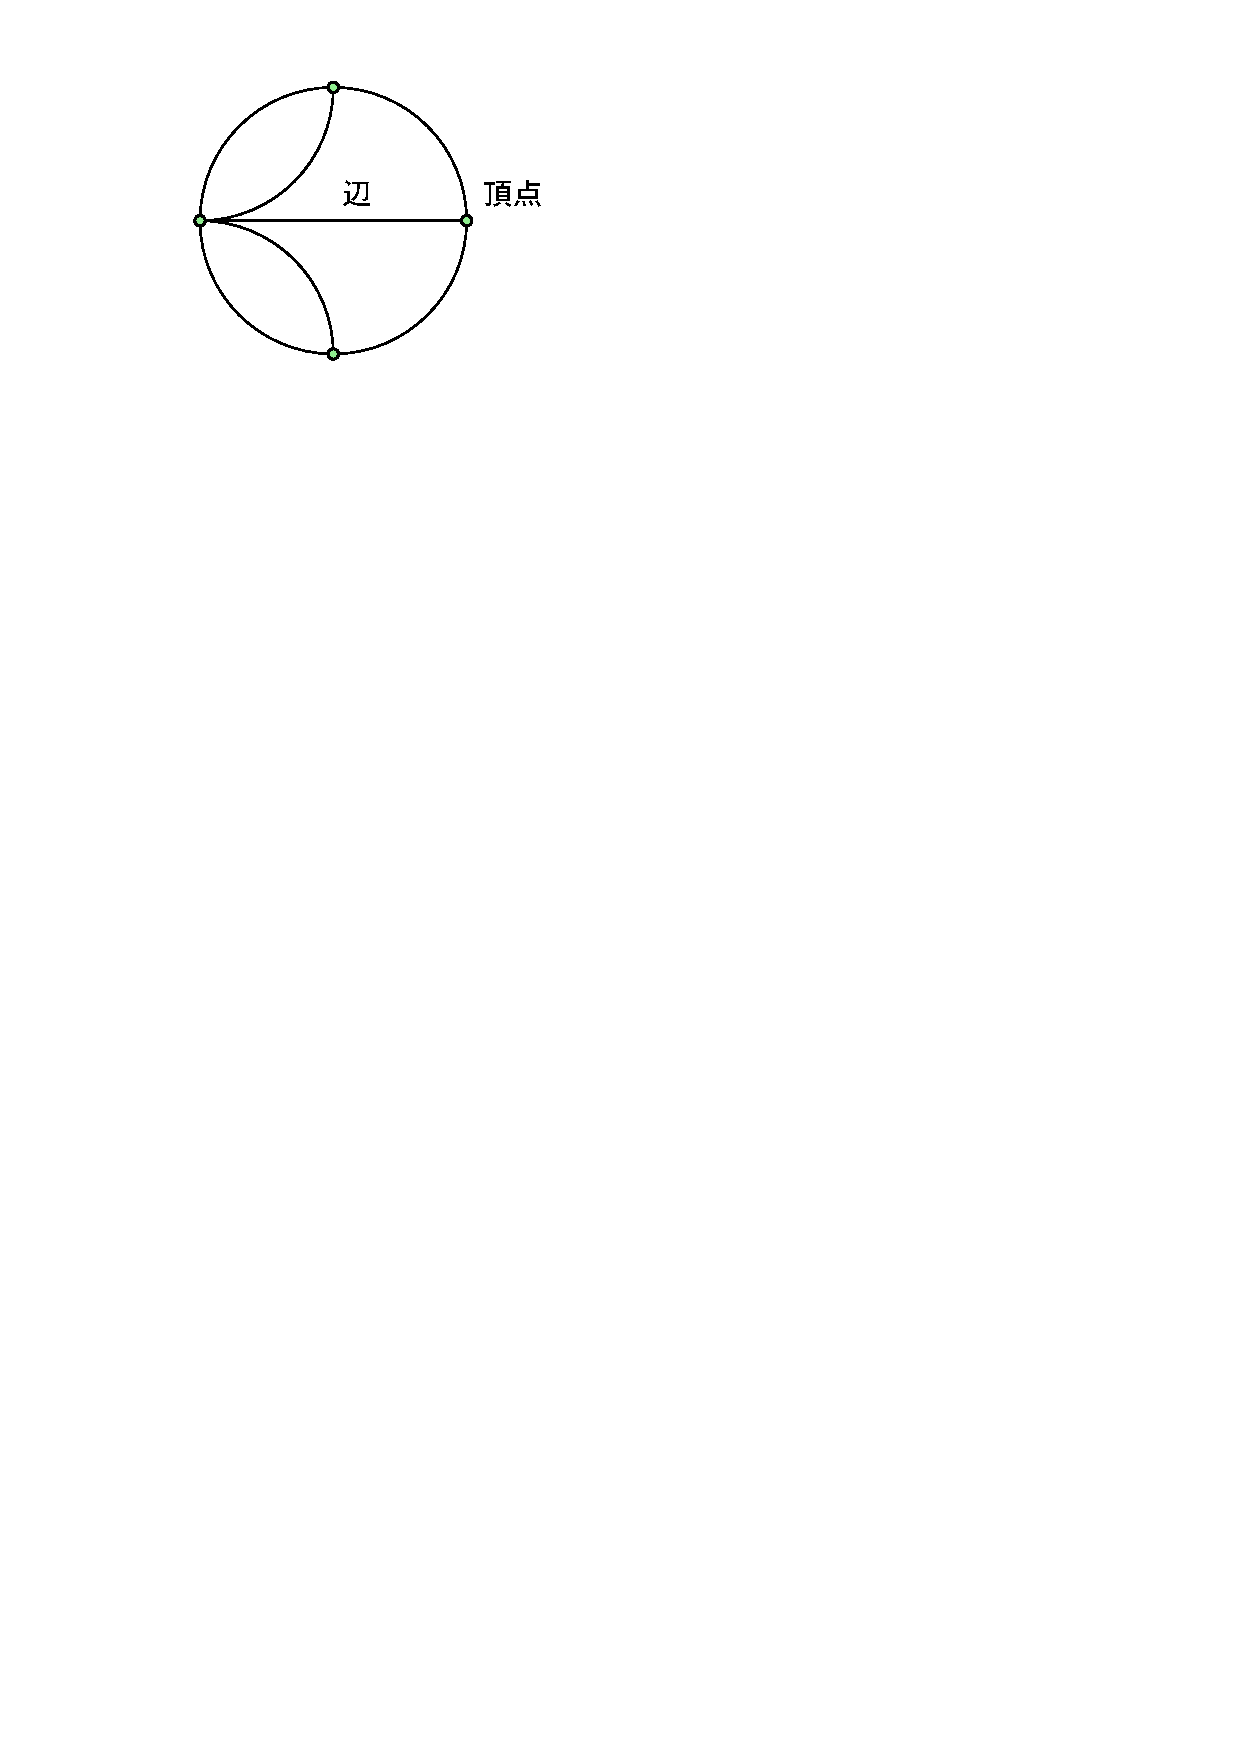
\includegraphics[width=0.15\textwidth]{figures/Konigsberg.pdf}\\
{\small ケーニヒスベルクの\\七つの橋}
\end{figure}
\end{paracol}




\setcolumnwidth{0.9\textwidth, 0.1\textwidth}
\begin{paracol}{2}
\paragraph{単純グラフ}
ある辺$e=(u, v)$が$u=v$の場合$e$を自己ループという。
グラフ$G=(V, E)$が単純であるという言及は、
$E$に自己ループや重複する辺を含まないことを意味する。
重複する辺を許す場合、それらの辺を多重辺と呼ぶ。
平面性を判定する際は、
自己ループや多重辺を削除もしくは細分した単純なグラフを対象とする。
\switchcolumn
%\vspace{-0.5\intextsep}
\begin{figure}[ht]
\centering

\includegraphics[width=0.09\textwidth]{figures/self_loop_and_multiedges.pdf}
\end{figure}
\end{paracol}


\setcolumnwidth{0.85\textwidth, 0.15\textwidth}
\begin{paracol}{2}
\paragraph{頂点と辺の近接性}
無向グラフ$G=(V, E)$において$e=(u, v)\in E$なら$u$と$v$は互いに隣接するという。
また、$e$は$u$と$v$を接続するという。
頂点$u$の隣接頂点の集合$N(u)$は
%$N(u) = \{v \mathrm{\ for\ } (u, v) \in E\}$のように記述できる。
$N(u) = \{v ~|~ (u, v) \in E\}$のように記述できる。
頂点$v$の次数を$\deg(v)$と書き$v$に接続する辺の個数とする。
$\deg(v) = |N(v)|$とも書ける。
$\deg(v)=0$の頂点$v$を孤立点という。

\switchcolumn
\vspace{1.0\intextsep}
\begin{figure}[ht]
\centering
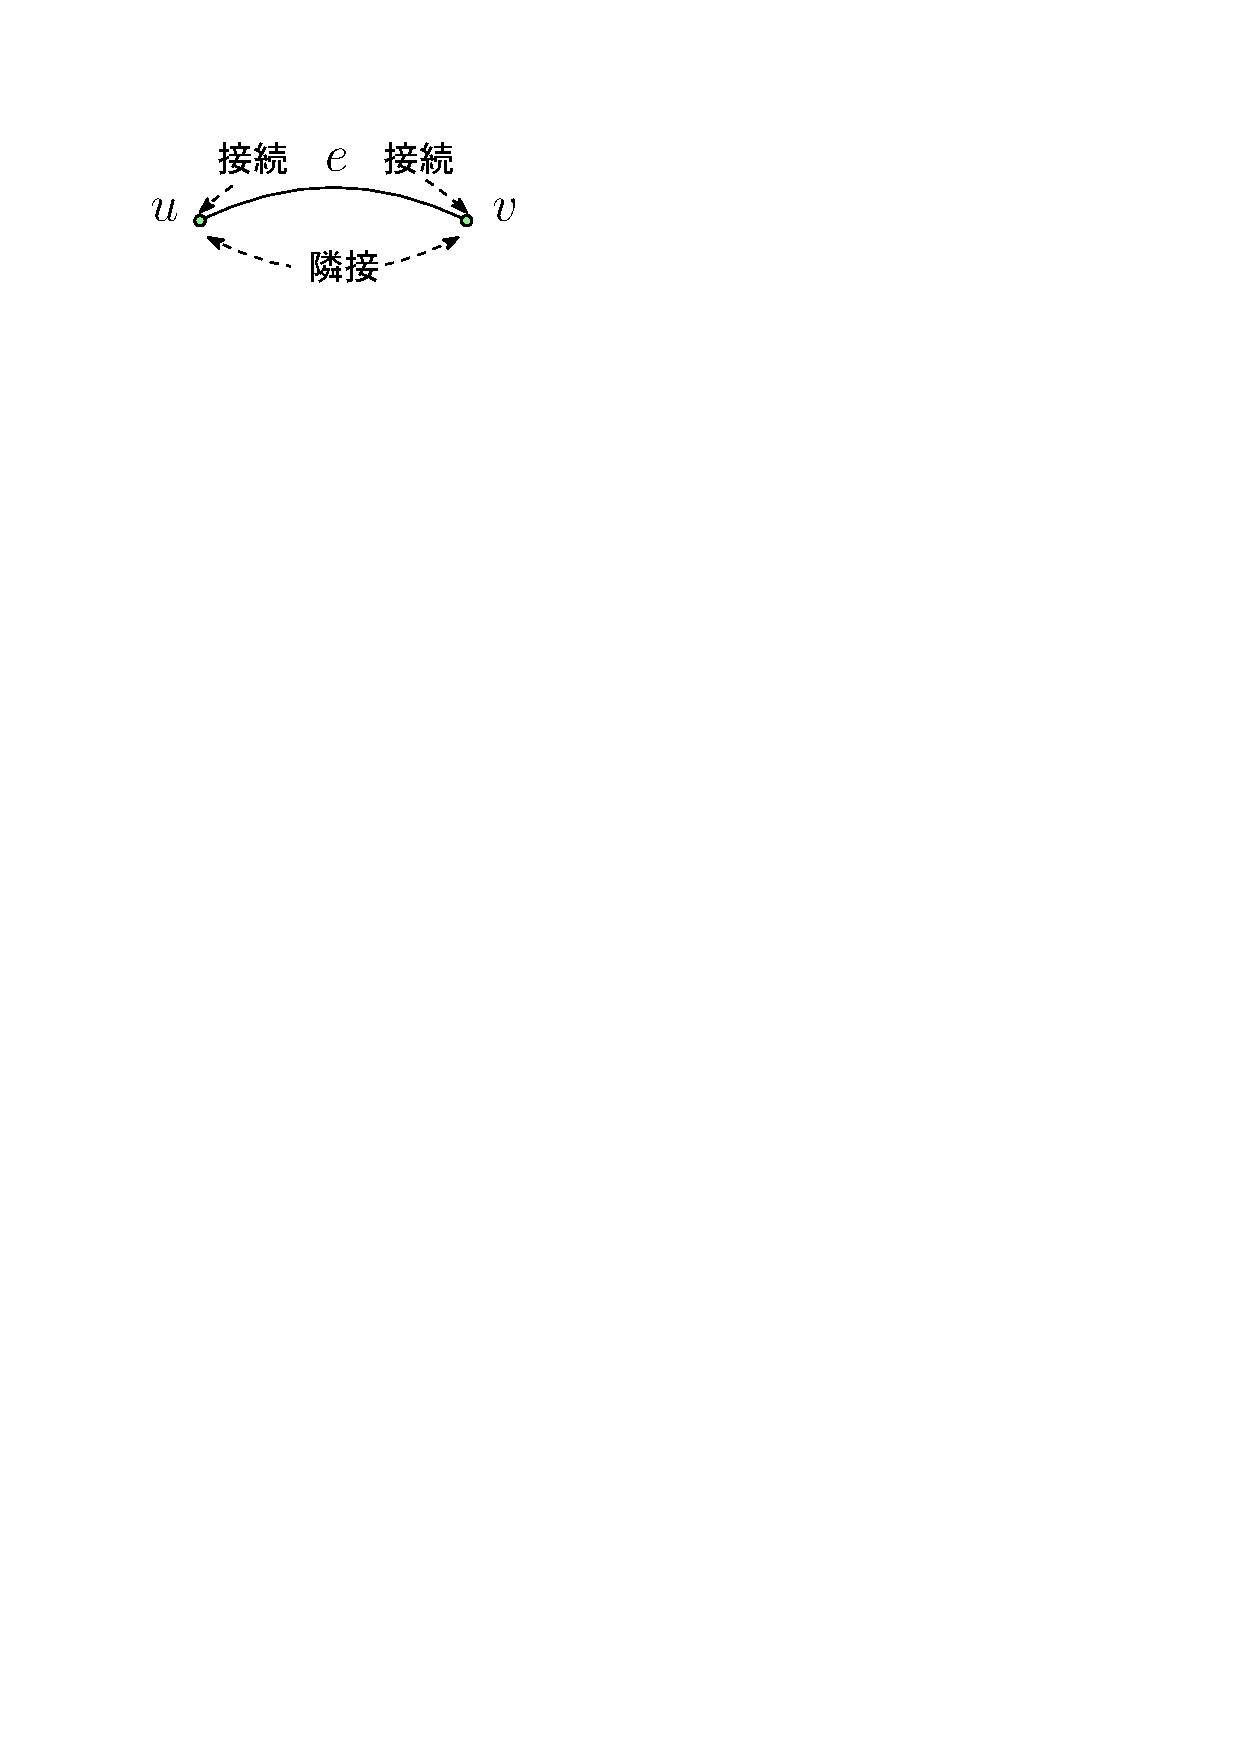
\includegraphics[width=0.14\textwidth]{figures/neighbors.pdf}
\end{figure}
\end{paracol}


\setcolumnwidth{0.8\textwidth, 0.2\textwidth}
\begin{paracol}{2}
\paragraph{完全グラフ}
すべての二頂点が隣接するグラフを完全グラフという。
つまり$G=(V, E)$に対して$E=V^2$。
$n$頂点の完全グラフを$K_n$と書く。
グラフ$G=(V_1 \cup V_2, E)$が、頂点集合を二つの互いに素な集合$V_1, V_2$に分割でき、
どの辺も$V_1$の頂点と$V_2$の頂点を接続するグラフを二部グラフという。
完全二部グラフはその辺集合が$E = V_1 \times V_2$となるグラフである。
$K_{n_1, n_2}$で$n_1, n_2 = |V_1|, |V_2|$の完全二部グラフを表す。
\switchcolumn
\vspace{0.5\intextsep}
\begin{figure}[ht]
\centering
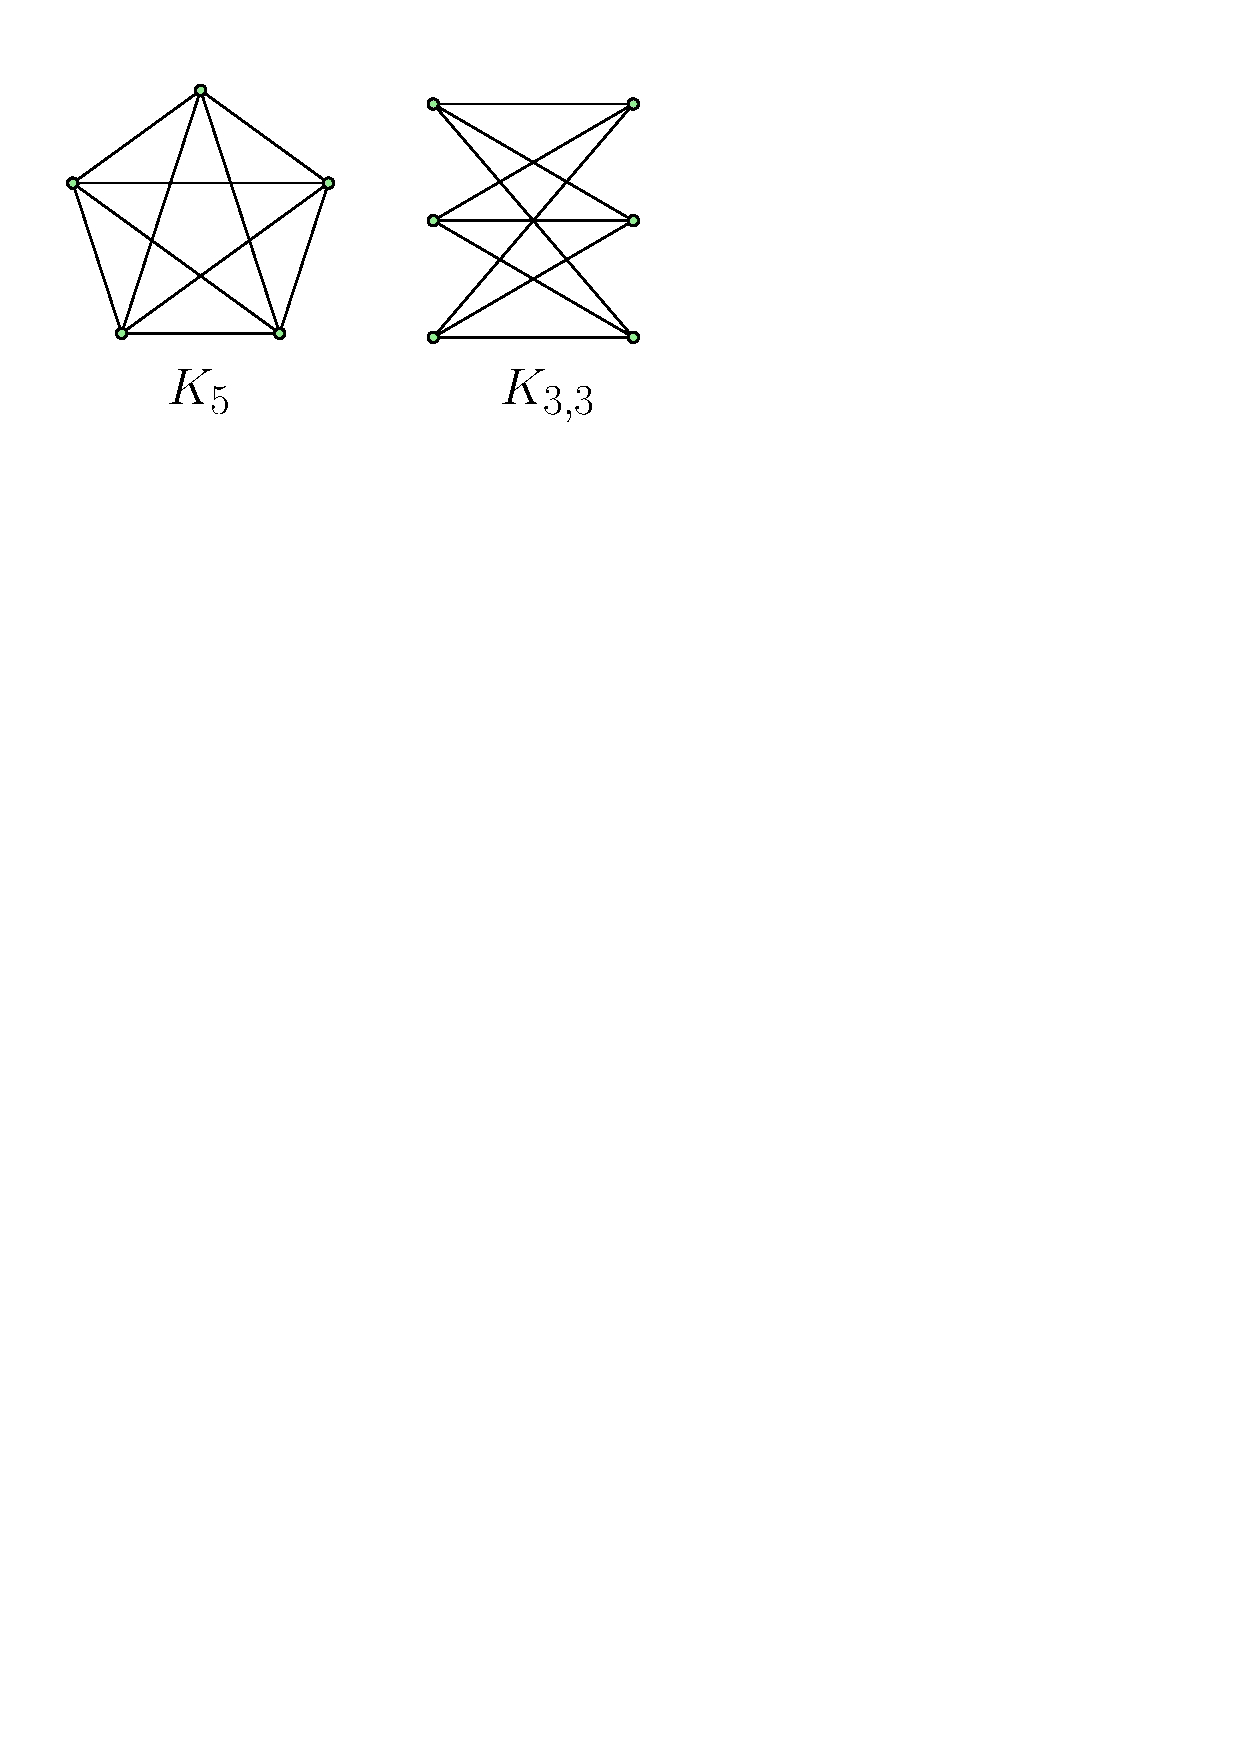
\includegraphics[width=0.19\textwidth]{figures/complete_graphs.pdf}
\end{figure}
\end{paracol}





%\vspace*{-0.7\intextsep}
\setcolumnwidth{0.7\textwidth, 0.3\textwidth}
\begin{paracol}{2}
\paragraph{グラフの局所編集(削除、縮約、細分)}
$G=(V, E)$からある辺$e \in E$を削除して得られるグラフを$G\setminus e$で表す。
$G\setminus e$は$e$以外の$G$の接続関係を継承する。
同様に$G\setminus v$で、
頂点$v\in V$と$v$に接続するすべての辺を削除することで得られるグラフを表わす。
二項演算子$\setminus$は集合の差演算に倣う。
また、
$S \subseteq V$や$T \subseteq E$に対して$G\setminus S$や$G\setminus T$の記述を許す。

辺$e$が自己ループや多重辺でないとき、
$e$の縮約は$e$の端点を併合して一つの頂点$v_e$としつつ$e$を削除する操作である。
このとき両端点に接続する$e$を除くすべての辺の接続関係を$v_e$に引き継ぐ。
自己ループや多重辺に縮約は適用できない。
$G / e$によって副次的に多重辺が生成されるが一般的にこれは削除され単純化される。
ただ、数学的帰納法など証明手順によっては敢えて多重辺を削除しないこともある。
$G / e$で$e$を縮約して得られるグラフを表す。
これも$T\subseteq E$に対して$G / T$のような記述を許す。

グラフの辺細分は、
ある一辺の内部を部分分割して二辺で置き換える操作である。
$K_{3,3}$もしくは$K_5$に対して有限回の辺細分を適用して得られるグラフを
クラトフスキーグラフという。
クラトフスキーグラフは、グラフの平面性を特徴付ける重要な役割を果たす。

\switchcolumn
\vspace{1.5\intextsep}
%\begin{figure}[ht]
\centering
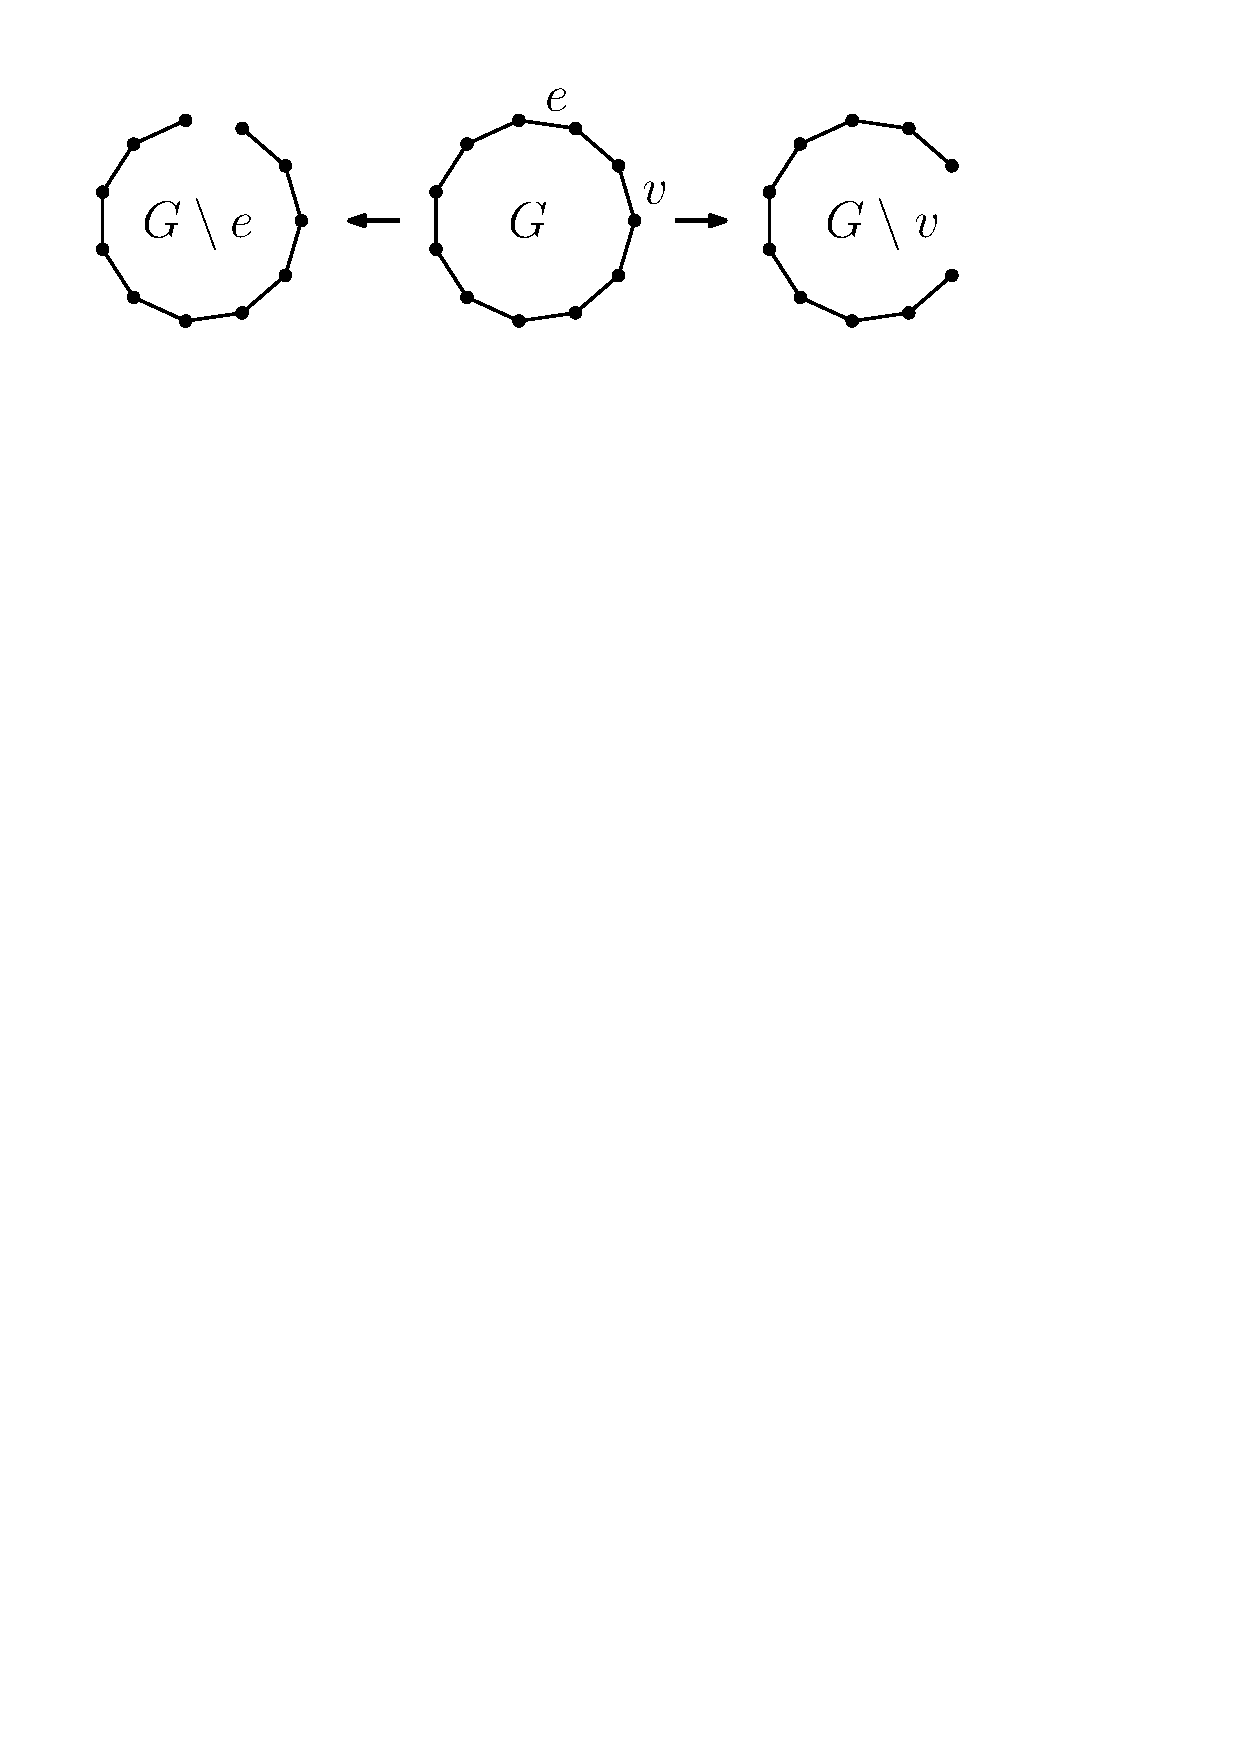
\includegraphics[width=0.29\textwidth]{figures/deleting.pdf}

\vspace{1.5\intextsep}
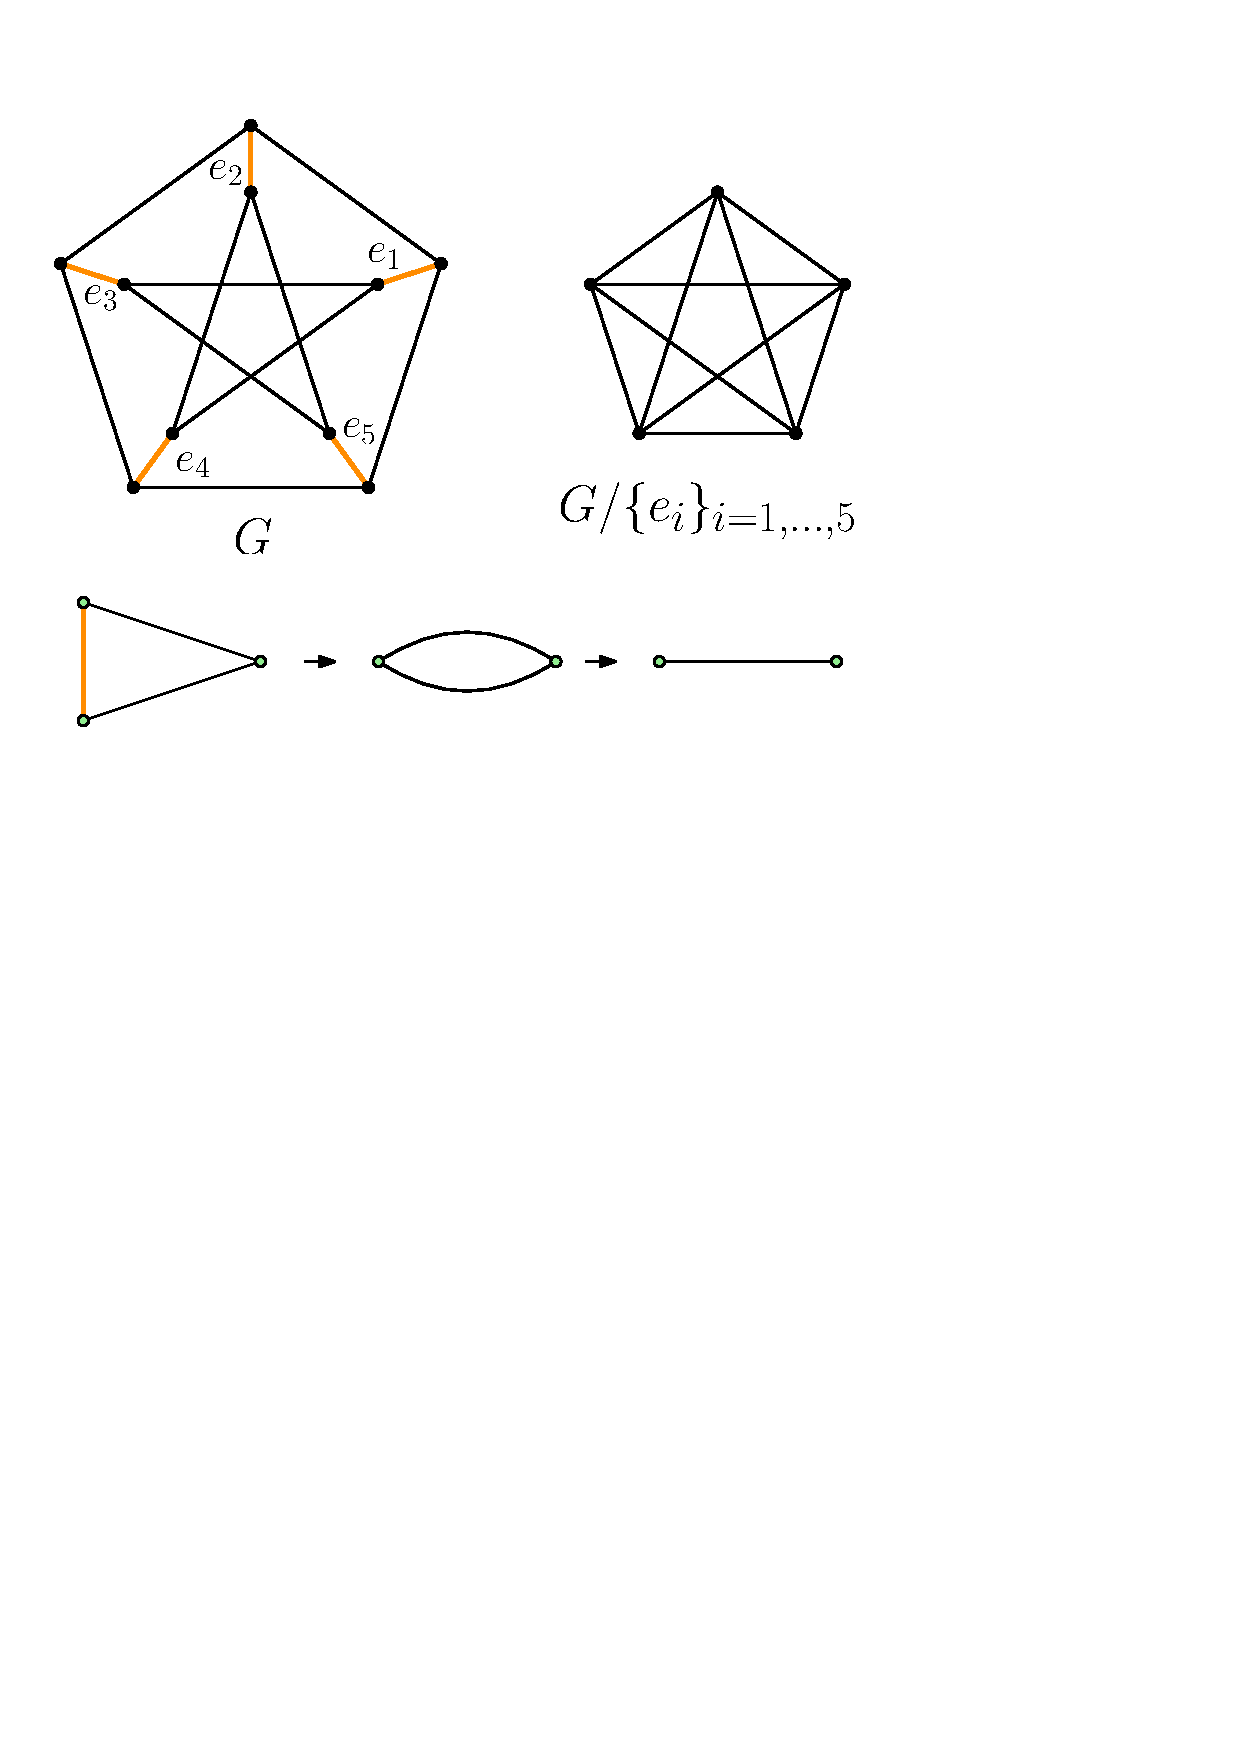
\includegraphics[width=0.20\textwidth]{figures/edge_contractions.pdf}

\vspace{1.\intextsep}
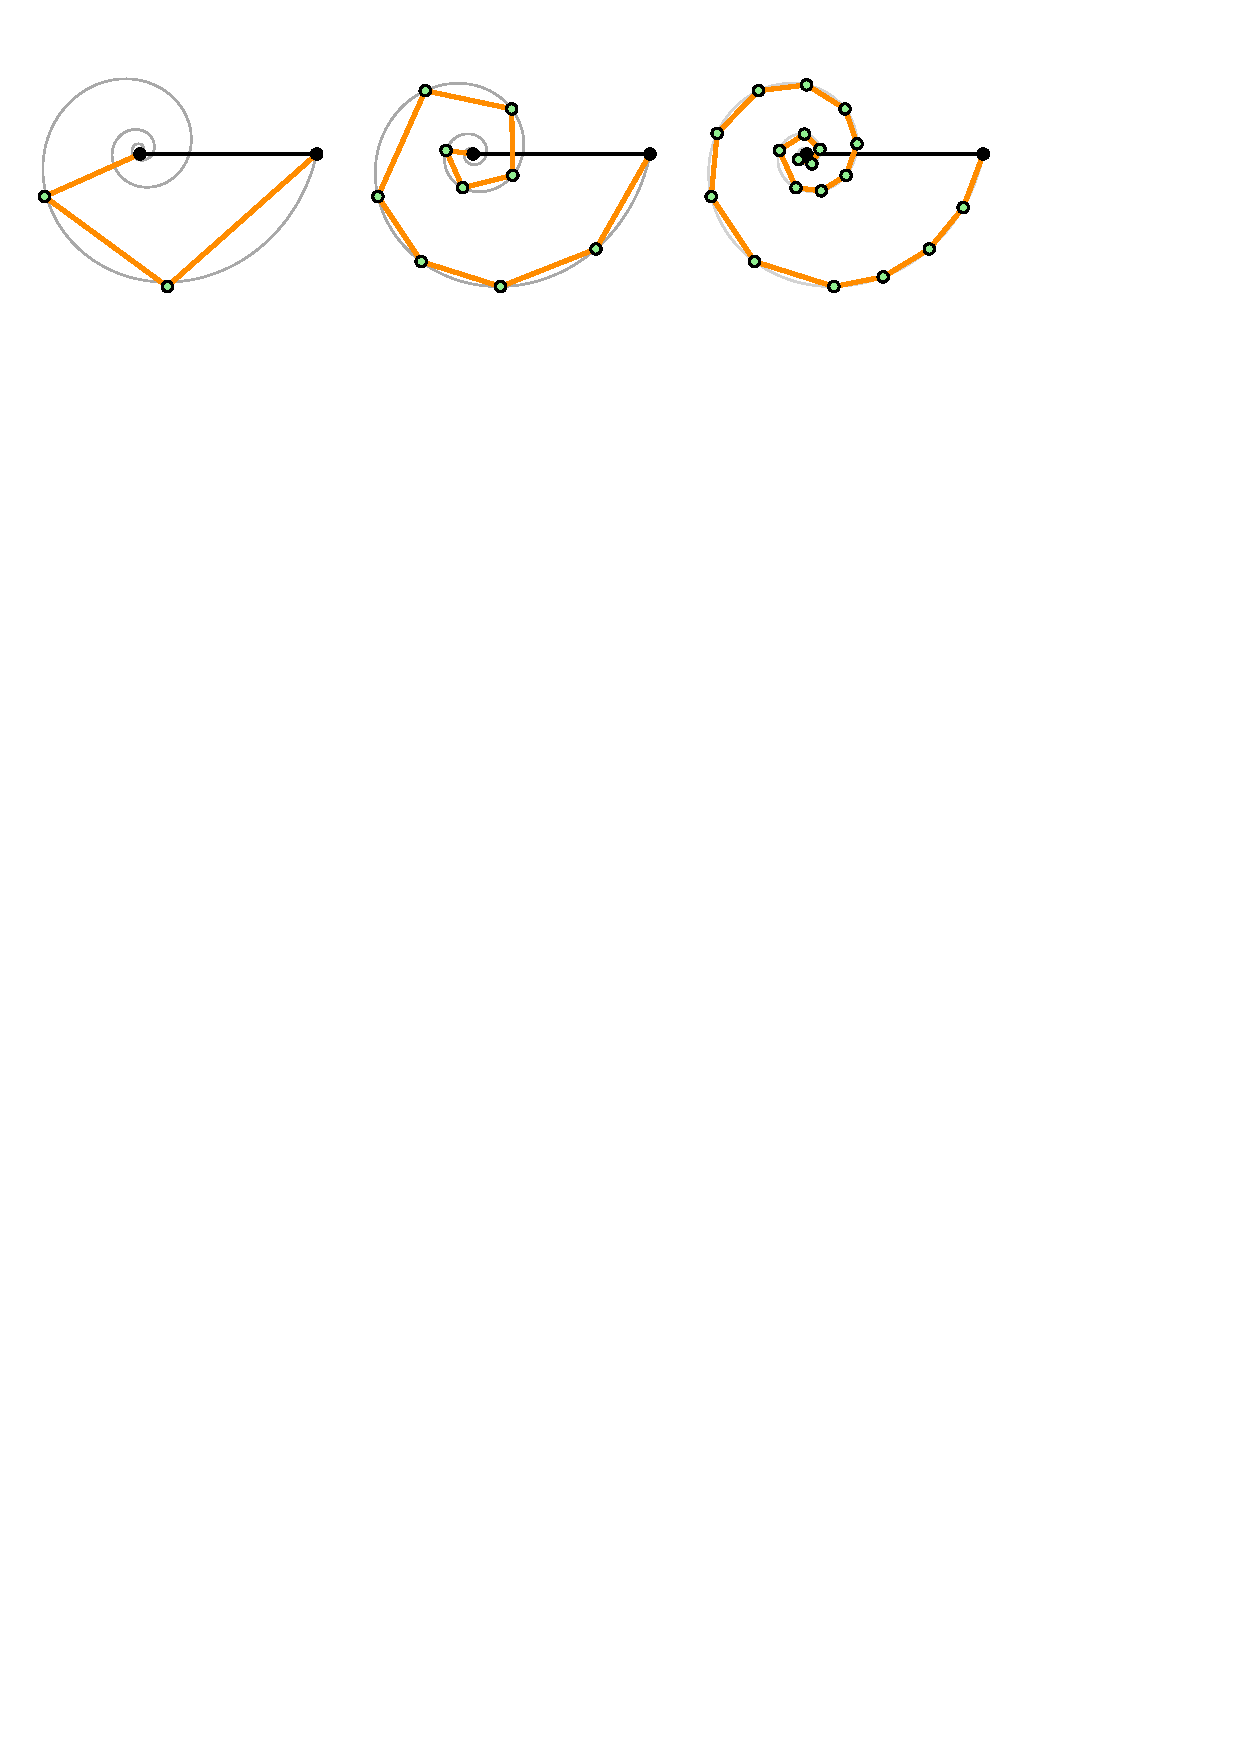
\includegraphics[width=0.29\textwidth]{figures/edge_subdivision.pdf}
%\end{figure}
\end{paracol}

\setcolumnwidth{0.7\textwidth, 0.3\textwidth}
\begin{paracol}{2}
\paragraph{グラフの集合演算と部分グラフ}
グラフ$G_1 = (V_1, E_1)$と$G_2=(V_2, E_2)$に対して
グラフの和を$G_1 \cup G_2 = (V_1 \cup V_2, E_1 \cup E_2)$とする。
同様にグラフの積を$G_1 \cap G_2 = (V_1 \cap V_2, E_1 \cap E_2)$とする。
あるグラフ$G$および$H$に対して$G \cup H = G$のとき$H$を$G$の部分グラフという。
任意の頂点集合$S \subseteq V$に対して、
頂点集合が$S$であり、辺集合が$E$の部分集合で両端点が$S$に含まれるものを
$G[S]$と書き$G$の誘導部分グラフという(右図右)。
また、任意の辺集合$T\subseteq E$が誘導するグラフ$G[T]$を
$G[T]=(V_T, T)$と定義する。
ただし$V_T=\bigcup\limits_{(x,y)\in T}\{x, y\}$。

\switchcolumn
%\vspace{1.5\intextsep}
\centering
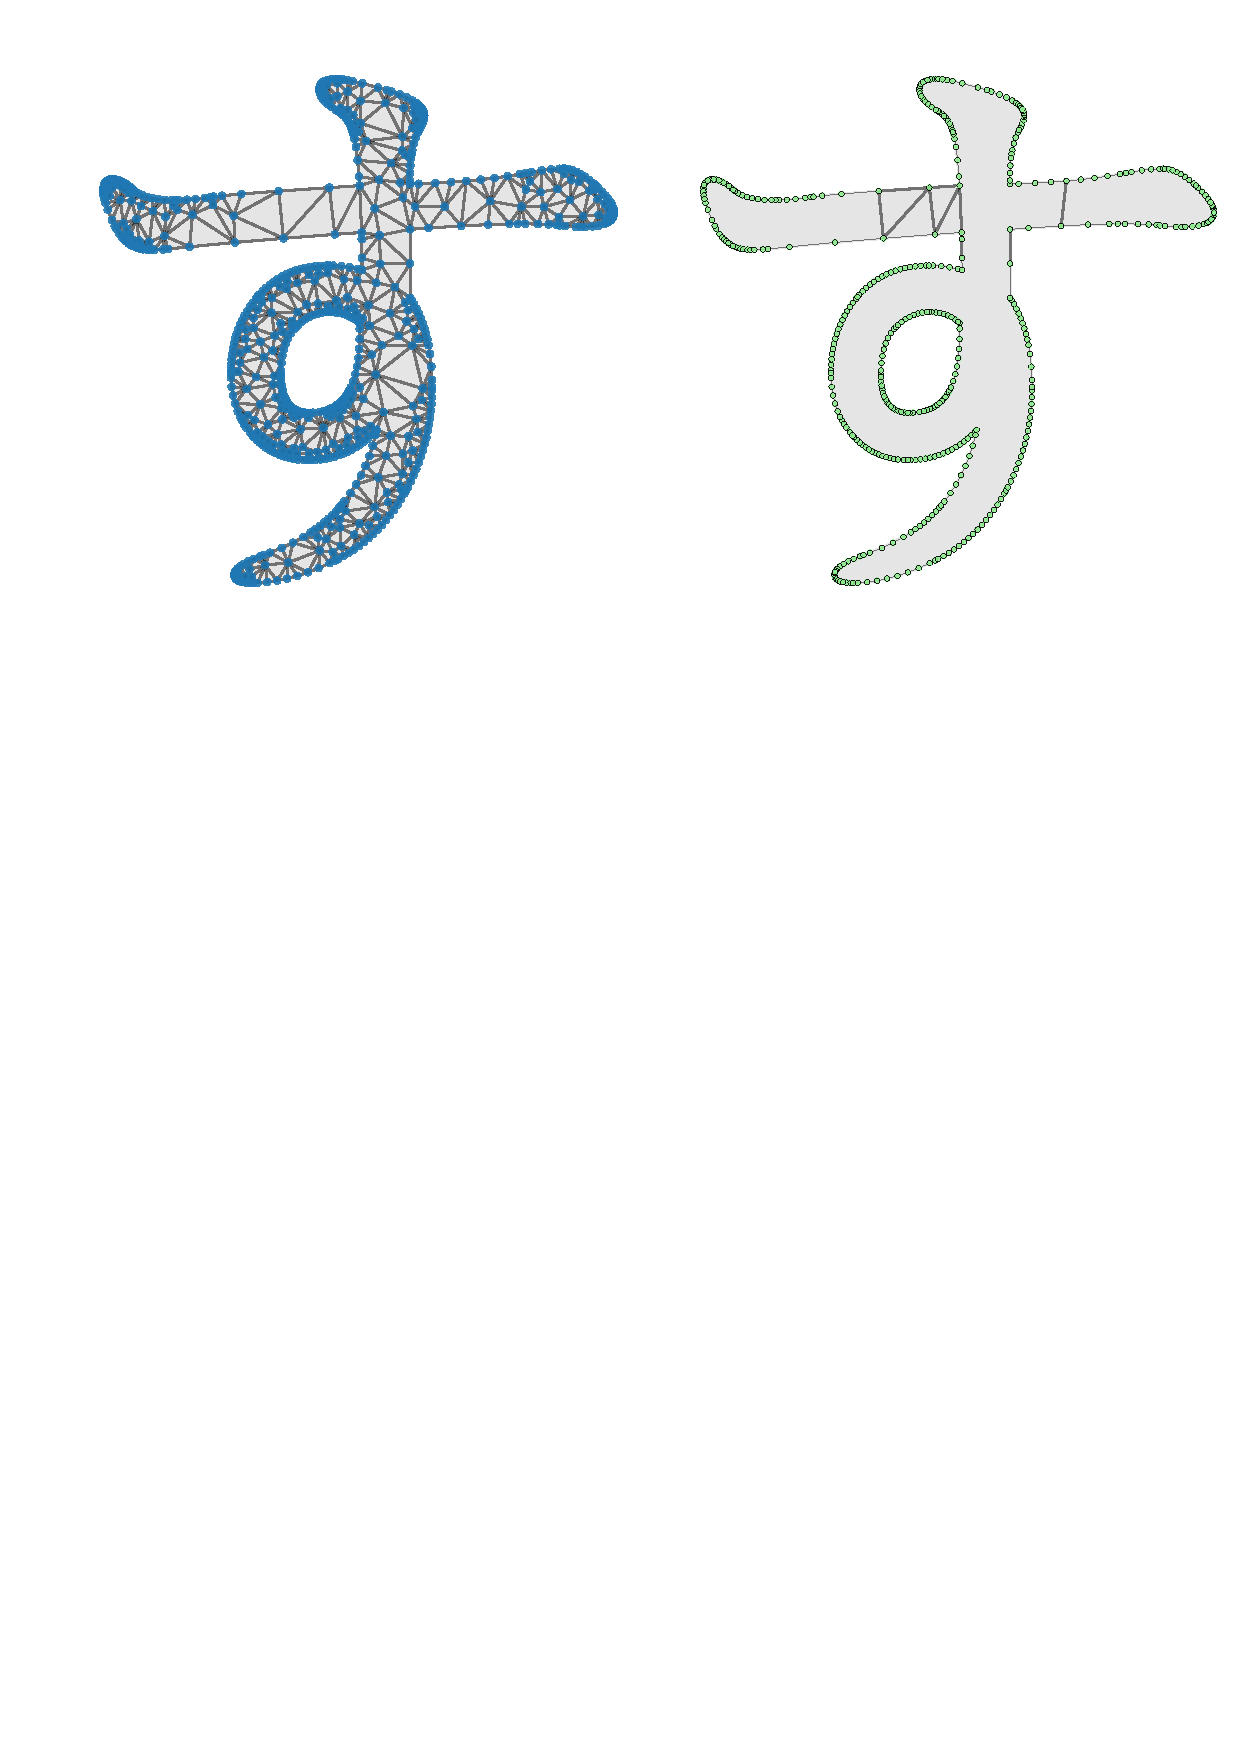
\includegraphics[width=0.29\textwidth]{figures/connect_su.pdf}

{\small ひらがな「す」のアウトラインの\\頂点集合を$S$とした際の
誘導部分グラフ$G[S]$。~~~~~~~~~~~~~~~~~~~~~~~~~}
\end{paracol}

\setcolumnwidth{0.85\textwidth, 0.15\textwidth}
\begin{paracol}{2}
\paragraph{経路と閉路}
次の条件を満たす頂点と辺の交互列を経路もしくはパスという。
始点と終点が異なる頂点で、
連続する頂点と辺は接続し、
いずれの頂点と辺も重複しない。
%始点と終点はそれぞれ交互列の先頭と末尾の頂点とする。
始点と終点が同じ経路を閉路という。
経路や閉路の長さは辺の個数で測られる。
一般的に任意の経路の長さは$1$以上だが
数学的帰納法を用いる証明手段や言語実装など、
頂点一つからなる長さ$0$の経路を許すと簡潔に記述できることがある。
無向グラフにおいて頂点$u, v$間に経路$p$が存在するなら、
$u$と$v$は互いに到達可能であるといい$p$は$u$と$v$を接続するという。
%同様に、有向グラフにおいては頂点$u$から$v$にパスが存在する場合
%$u$から$v$へ到達可能であるという。
グラフ内の最小閉路の長さを\hlpink{内周}という。
閉路を持たないグラフの内周は$\infty$とする。


\switchcolumn
\vspace{1.5\intextsep}
\centering

\includegraphics[width=0.14\textwidth]{figures/paths.pdf}
\end{paracol}




\setcolumnwidth{0.7\textwidth, 0.3\textwidth}
\begin{paracol}{2}
\paragraph{グラフの連結性}
無向グラフが\hlpink{連結}であるという言及は
任意の二頂点が互いに到達可能であることを意味する。
逆に互いに到達可能でない頂点対が一つでもあれば、そのグラフは\hlpink{非連結}であるという。
非連結なグラフ内の連結な部分グラフを\hlpink{連結成分}という。
ある頂点$v$をグラフから削除すると非連結になるとき$v$を\hlpink{切断点}という。
同様に、ある辺$e$の削除で非連結になるなら$e$を\hlpink{橋}という。
閉路を持たない連結なグラフを木という。
木における頂点および辺は、いずれも切断点であり、橋である。
平面性判定は連結成分ごとに実行すれば良いので、
%以下では断りが無い限り入力として与えられるグラフは連結グラフとする。
以下では対象グラフは連結とする。

\switchcolumn
%\begin{figure}[ht]
\vspace{1.5\intextsep}
\centering

\includegraphics[width=0.29\textwidth]{figures/connect_ai.pdf}
%\end{figure}
\end{paracol}


境界条件には瑣末だが注意が必要である。
一つの頂点のみからなるグラフを\hlpink{自明なグラフ}という。
一般的に自明なグラフには連結・非連結の概念は導入されない。
ただ、自明な部分グラフとしての孤立点は$0$-連結成分として
他の成分とは区別されることがある。
いずれにしても、平面性判定において頂点数が$4$以下のグラフは
すべて平面的なので、自明なグラフは本質的に対象外にできる。
%グラフの平面性に関しては、
%以下の平面描画の定義から自明なグラフおよび孤立点は平面的になる。



%\paragraph{全域木}
%根付き木$T$は閉路を持たない連結なグラフで、根と呼ばれる頂点を一つ持つ。





\setcolumnwidth{0.75\textwidth, 0.25\textwidth}
\begin{paracol}{2}
\paragraph{平面描画と平面埋込み}
あるグラフ$G$の\hlpink{描画}$\Gamma$は、
各頂点$v$を平面${\mathbb R}^2$上の点$\Gamma(v)$へ、
各辺$(u, v)$を$\Gamma(u), \Gamma(v)$を端点とするジョルダン開曲線へ写像する関数である。
ジョルダン曲線は自己交差しない平面曲線で、
開という形容は端点が異なることを意味する。
\hlpink{平面描画}は二つの異なる辺の写像が交差しないことをいう。
ただし共通して持つ端点で接することは許される。
平面描画を持つグラフを\hlpink{平面的グラフ}という。
任意の平面描画は平面を連続な領域に部分分割する。
%集合$S$の部分分割$\{S_1, \ldots, S_k\}$は、$S = \bigcup_{S_i \in S} S_i$かつ、
%任意の$i, j~(i \neq j)$に関して$S_i \cap S_j = \varnothing$を満たす
%$S$の部分集合満の集まりである。
この部分領域を\hlpink{面}という。
また、非有界な領域を\hlpink{外面}という(右図$f_0$)。

あるグラフの描画は無限に存在するが、
等価な描画を類別することで表現方法は有限個に限定される。
ある描画が与えられたとき、
各頂点に関して接続する辺を例えば時計回りのような一定の基準に則って
順序付けた構造を\hlpink{組合せ埋込み}という。
二つの描画が等価であるというのは、等価な組合せ埋込みを持つことで、
すべての頂点の接続辺の回転順序が辞書式で一致することを意味する。
平面描画を与える組合せ埋込みを\hlpink{平面埋込み}という。



\switchcolumn
\centering
\vspace{0.5\intextsep}
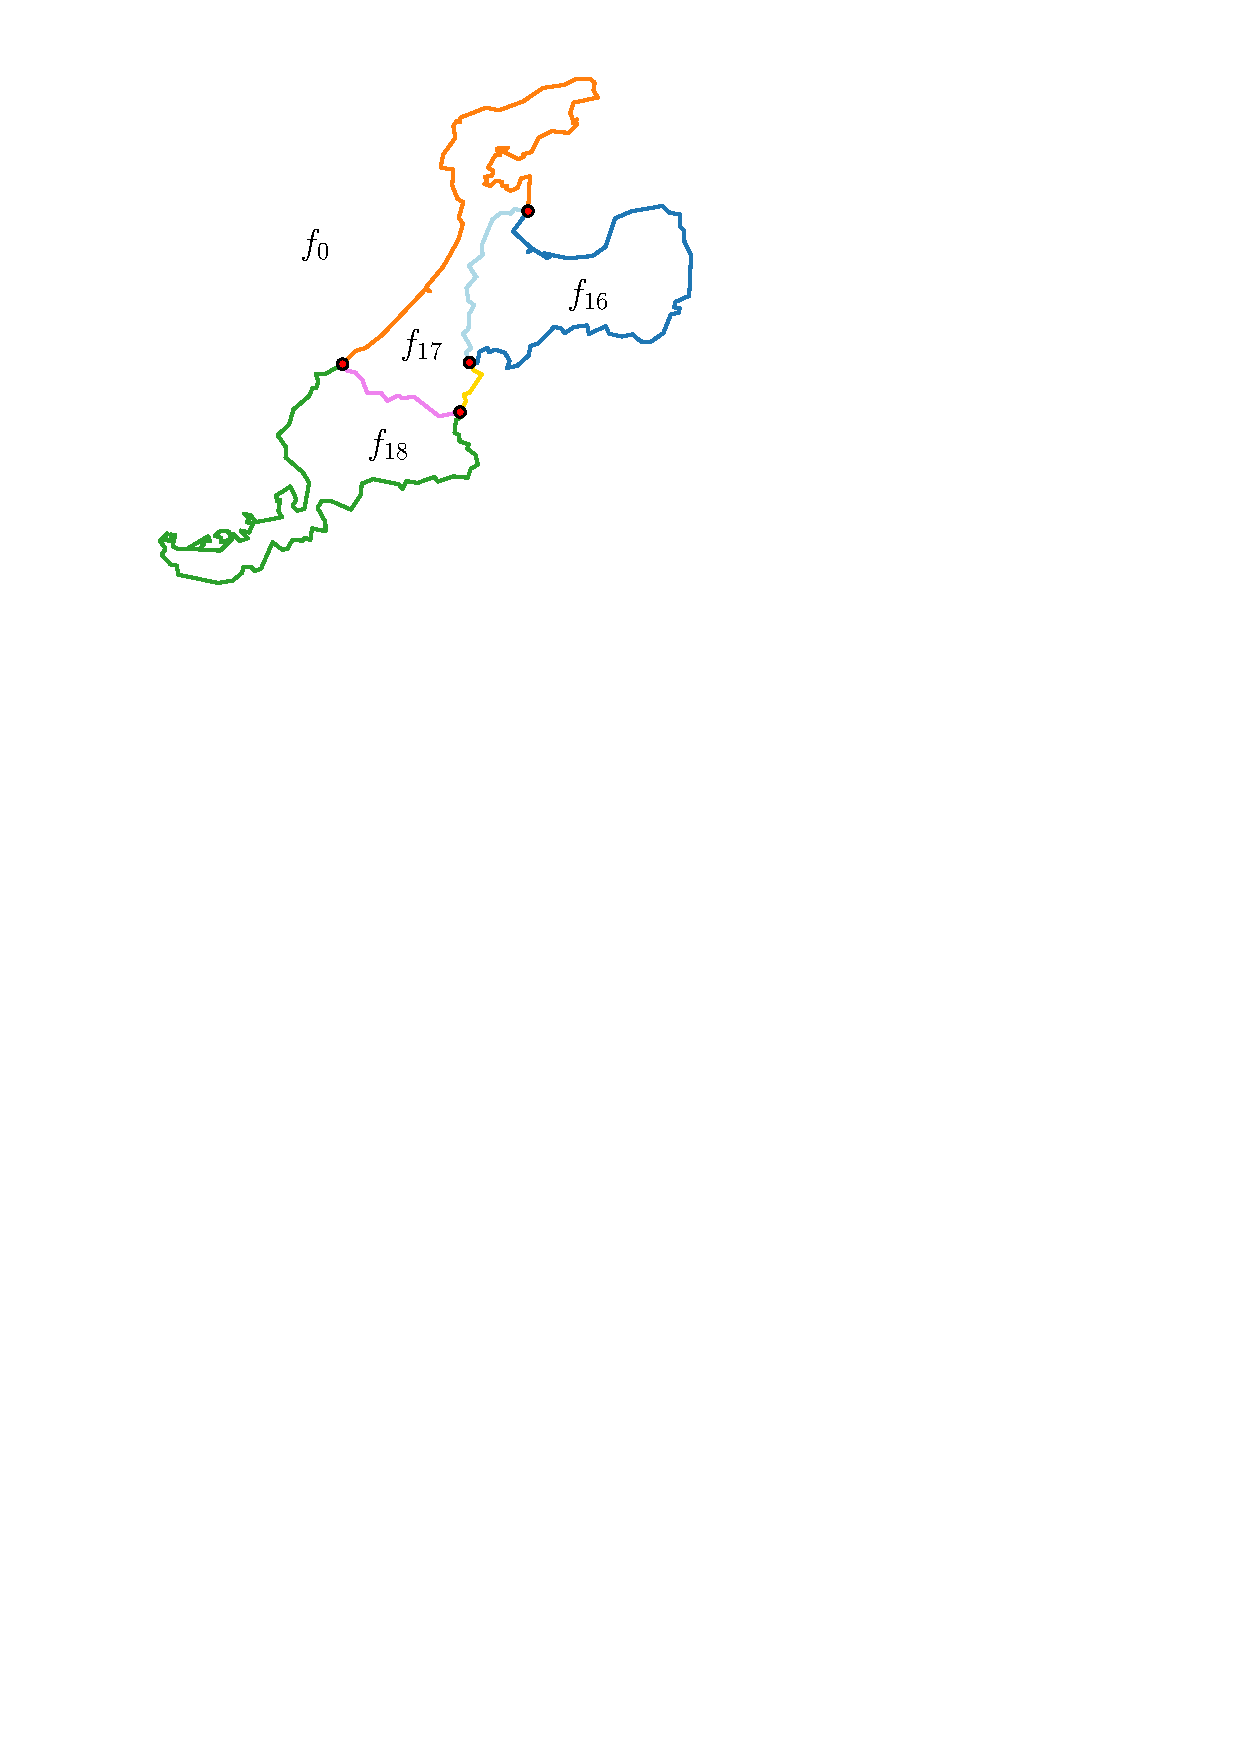
\includegraphics[width=0.24\textwidth]{figures/planar_drawing.pdf}

\vspace{1.\intextsep}
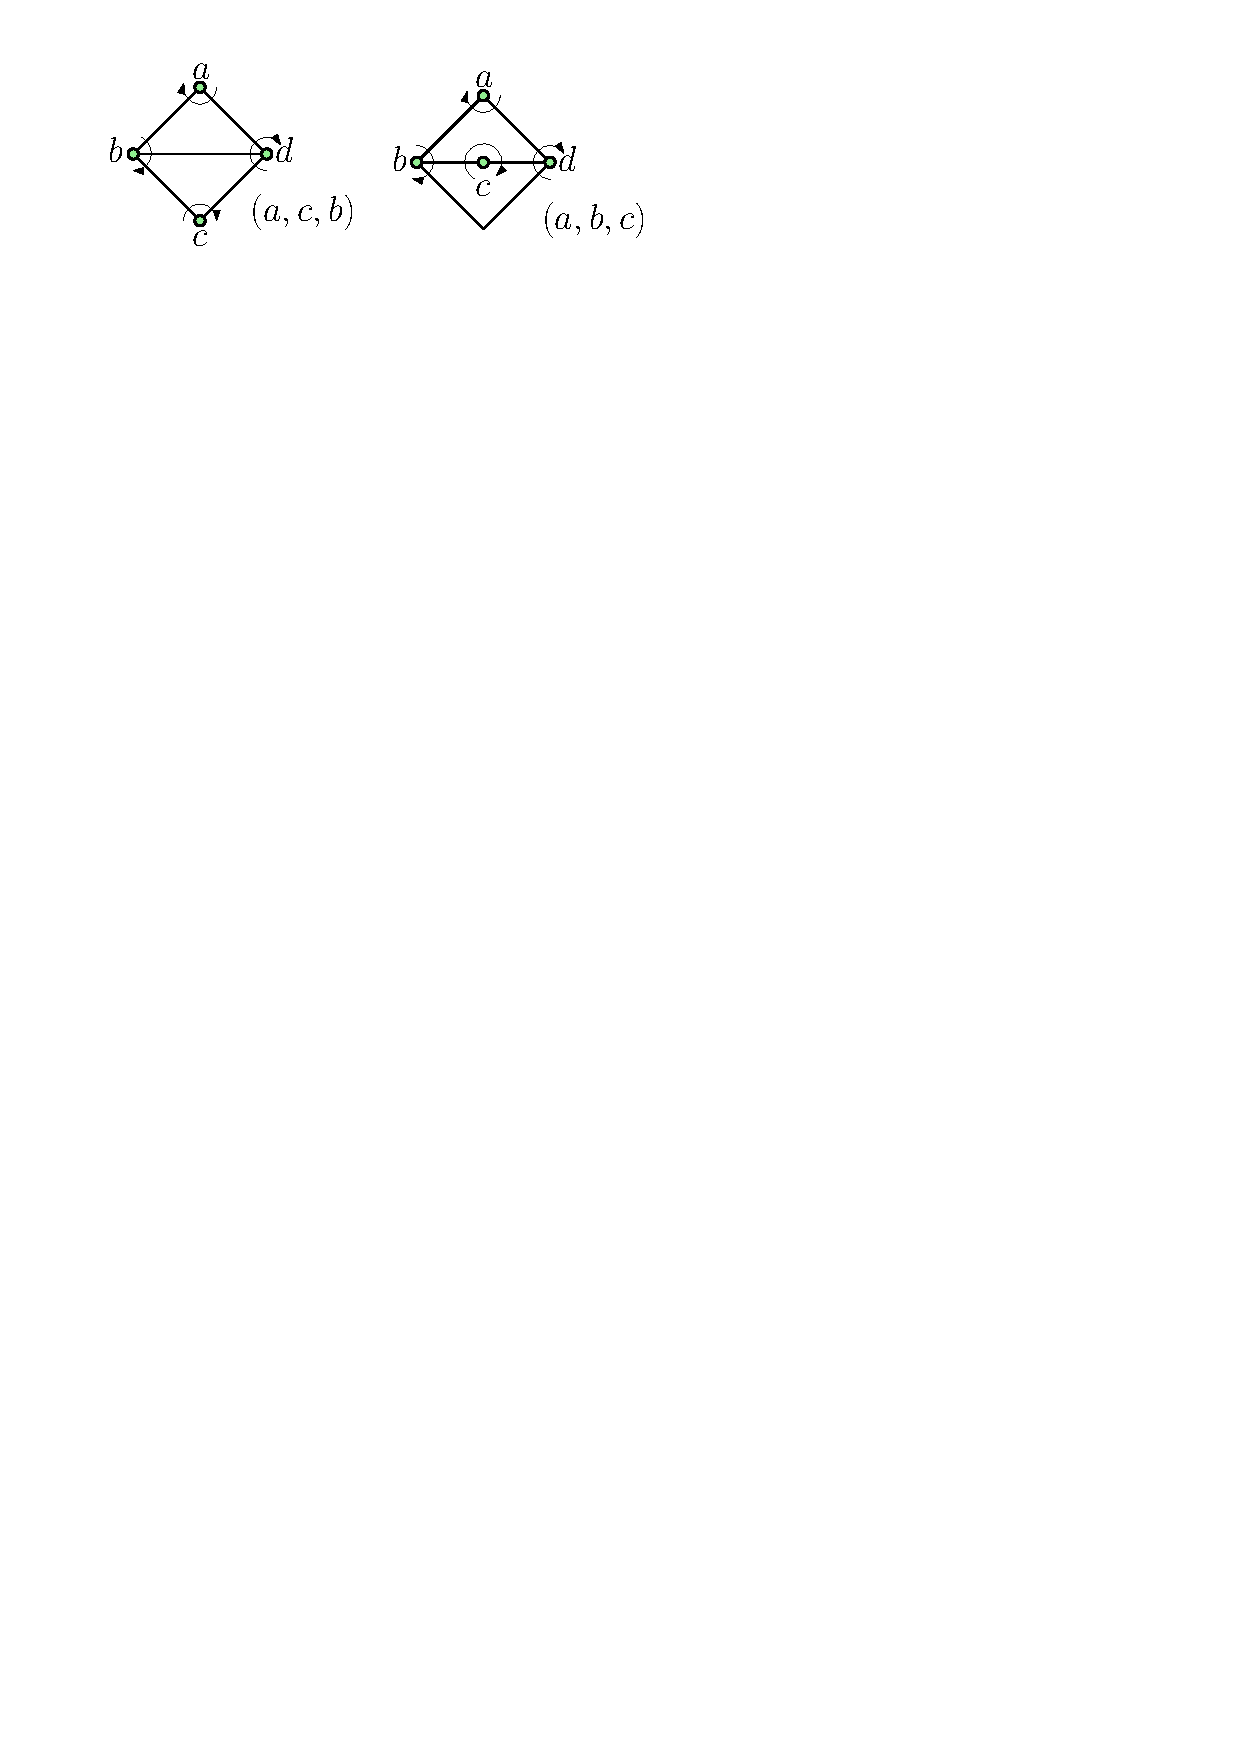
\includegraphics[width=0.24\textwidth]{figures/combinatorial_embedding.pdf}

\end{paracol}



\paragraph{極小性と極大性}
ある制約を満たす集合$S$が極小性を有するとは
$S$の要素を一つでも削除すると制約を満たさなくなることをいう。
同様に、極大性は$S$に要素を追加すると不成立になる飽和状態をいう。
例えば、辺集合が誘導する部分グラフの平面性に対する極小性と極大性を考える。
平面的なグラフから辺を削除しても平面性は損なわないが追加すると非平面的になり得るので
極大な平面的グラフを考えることができる。
極大な平面的グラフはその平面描画のすべての面が三辺で構成されるグラフとなる。
一方で極小な非平面的グラフはクラトフスキーグラフとなる
(クラトフスキーの\cref{thm:kuratowski})。


\newpage

\section{平面的なグラフの性質}

グラフの平面性を特徴付ける性質は1930年に
ロシアの数学者クラトフスキーが初めて正確に記述した。
その後約半世紀を経て平面性を判定する線形時間アルゴリズムが提案され、
言語実装に至ったのは90年代。
現在は様々な定理・補題を礎に100行程度で記述できるまで簡潔になっている。
ここでは代表的な三つの定理を通して平面的グラフの基本的な性質を確認する。



\subsection{オイラーの多面体公式}
オイラーの多面体公式は、
グラフが非平面的であることの緩い必要条件を記述する側面を持つ。
辺の個数が$3n-6$より多ければ非平面的と判定できる。
ただし$3n-6$以下のグラフであっても非平面的なグラフは存在するため、
緩い必要条件でグラフを平面的と決めつける判定方法は偽陽性を持つ。


\begin{theorem}[オイラーの多面体公式]
連結な平面的グラフ$G$が$n$個の頂点、$m$個の辺、そして
$f$個の面で構成されているとき、$n - m + f = 2$ が成り立つ。
\end{theorem}
\vspace*{-0.7\intextsep}
\setcolumnwidth{0.666\textwidth, 0.333\textwidth}
\begin{paracol}{2}
\begin{proof}
$G$ が辺を持たない自明なグラフなら%$n=f=1,~m=0$で
$1+0+1=2$。
辺の個数が$m-1$の任意の連結な平面的グラフで主張が成り立つと仮定する。
$G$の任意の辺$e$に関して次の二つの重複する場合分けを考える。

$e$が自己ループでも多重辺でもないなら$e$の縮約$G / e$は
$n-1$個の頂点と$m-1$個の辺、$f$個の面を持つ。
ただし、この辺縮約は副次的に生成される多重辺を削除しないものとする。
また、$e$ が橋でないなら$e$を削除して得られるグラフ$G \setminus e$は
$n$個の頂点、$m-1$個の辺、そして$f-1$個の面を持つ。
いずれも帰納法の仮定から$n - m + f = 2$を得る。
\end{proof}

\switchcolumn
%\vspace{.5\intextsep}
\centering
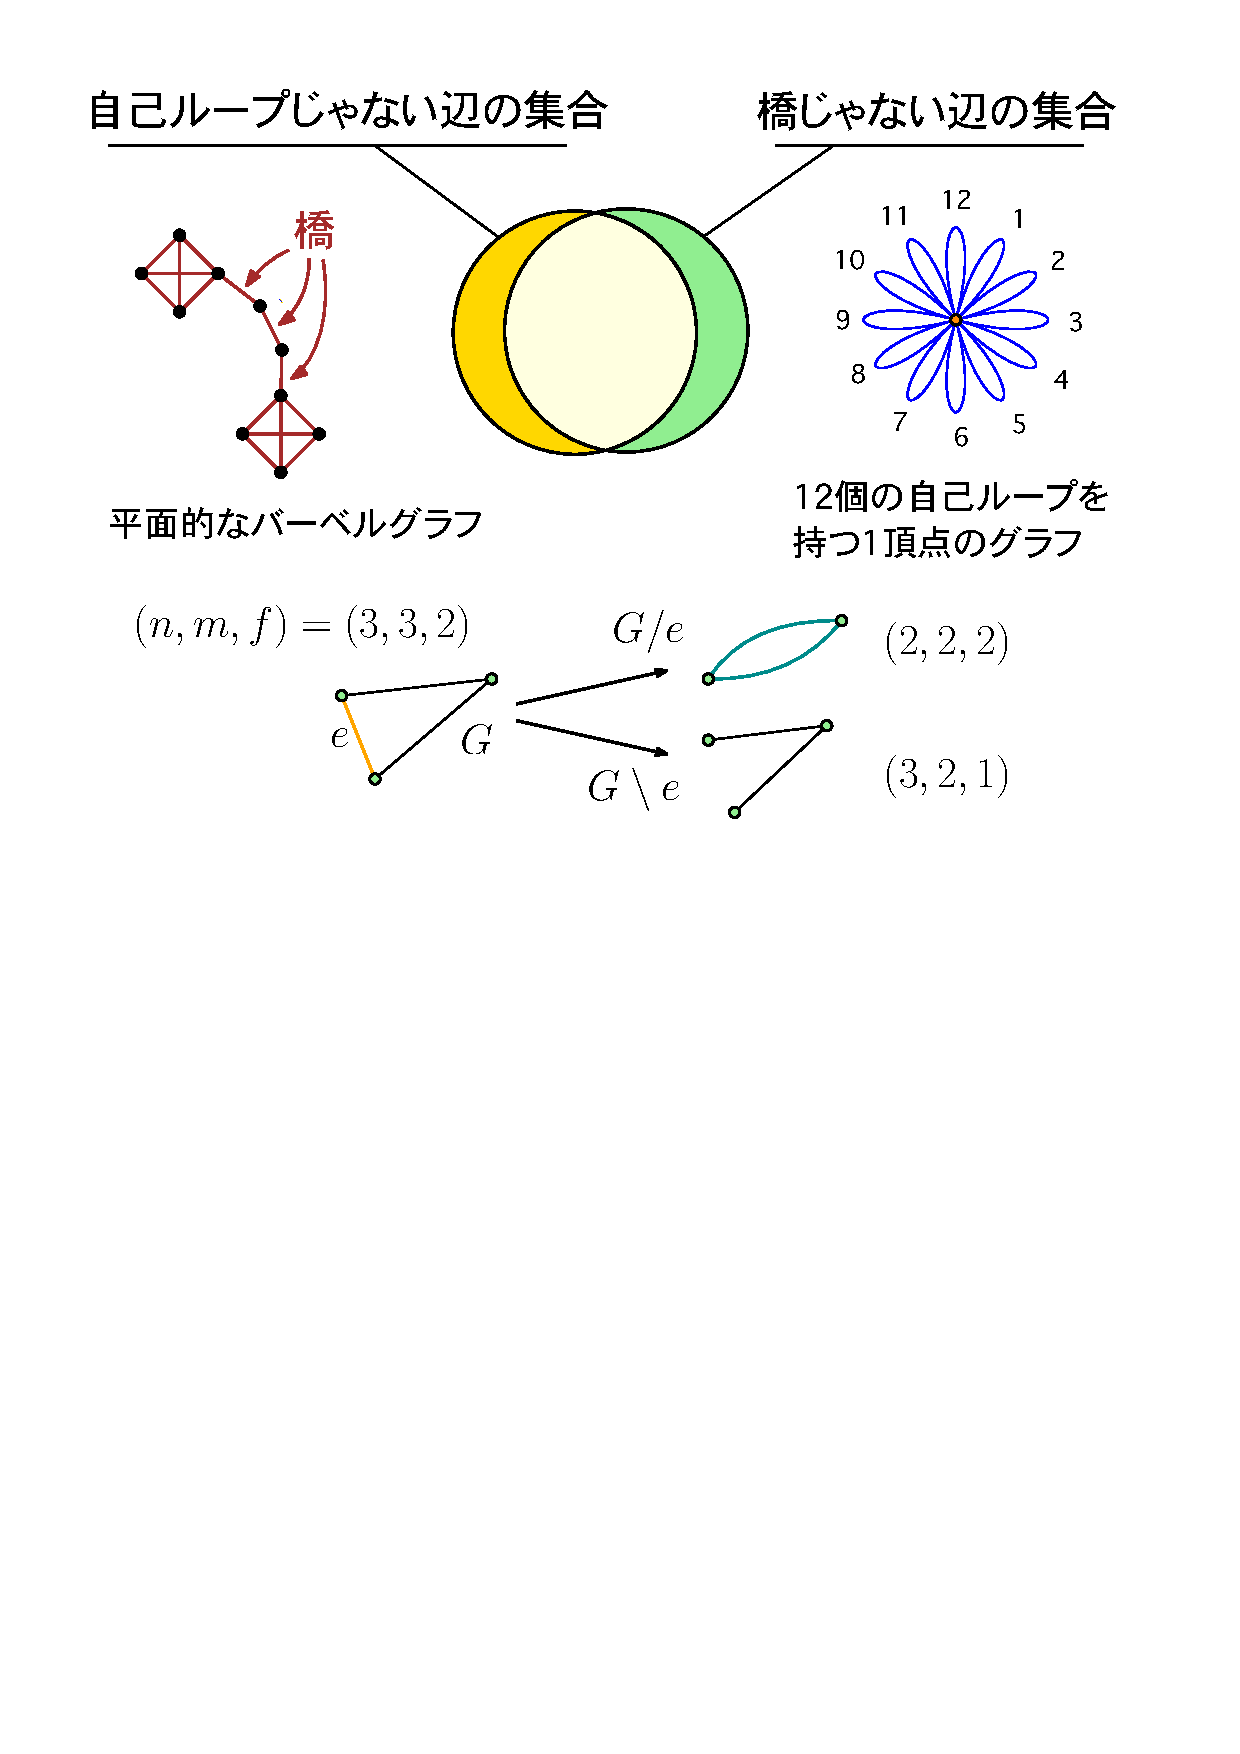
\includegraphics[width=0.32\textwidth]{figures/sample_figure_in_proof_of_eular_formula.pdf}
\end{paracol}



\begin{corollary}
\label{coro:girth}
単純で連結な平面的グラフ$G=(V, E)$が$|V|\geq 3$で、
内周が定数$\gamma$で抑えられるなら
$|E| \leq \frac{\gamma}{\gamma - 2}(|V| - 2)$が成り立つ。
\end{corollary}

\begin{proof}
握手補題からの類推より$\gamma |F| \leq 2|E|$を得る。
オイラーの多面体公式より$|V|-|E|+\frac{2}{\gamma}|E| \geq 2$。
この式を整理すると主張を得る。
\end{proof}

\begin{lemma}[握手補題]
グラフ$G=(V, E)$の次数の合計は辺の個数の$2$倍、
すなわち$\sum\limits_{v \in V}\deg(v)=2|E|$。
\end{lemma}
\vspace*{-0.7\intextsep}
\begin{proof}
各頂点の接続辺数を数え上げると、どの辺も二回カウントされる。
\end{proof}

\begin{corollary}
\label{coro:minimum_nonplanar}
最小頂点数の非平面的グラフは$K_5$。最小辺数の非平面的グラフは$K_{3,3}$。
\end{corollary}


\begin{proof}
$K_5, K_{3,3}$いずれも\cref{coro:girth}より非平面的。
下に連結な単純グラフで$5$頂点以下、
もしくは$6$頂点以上でも$9$辺以下で$2$-連結のグラフを示す。
$K_5$および$K_{3,3}$以外はいずれも平面描画を持つ。
\end{proof}

%\vspace*{.5\intextsep}
%\centering
\noindent
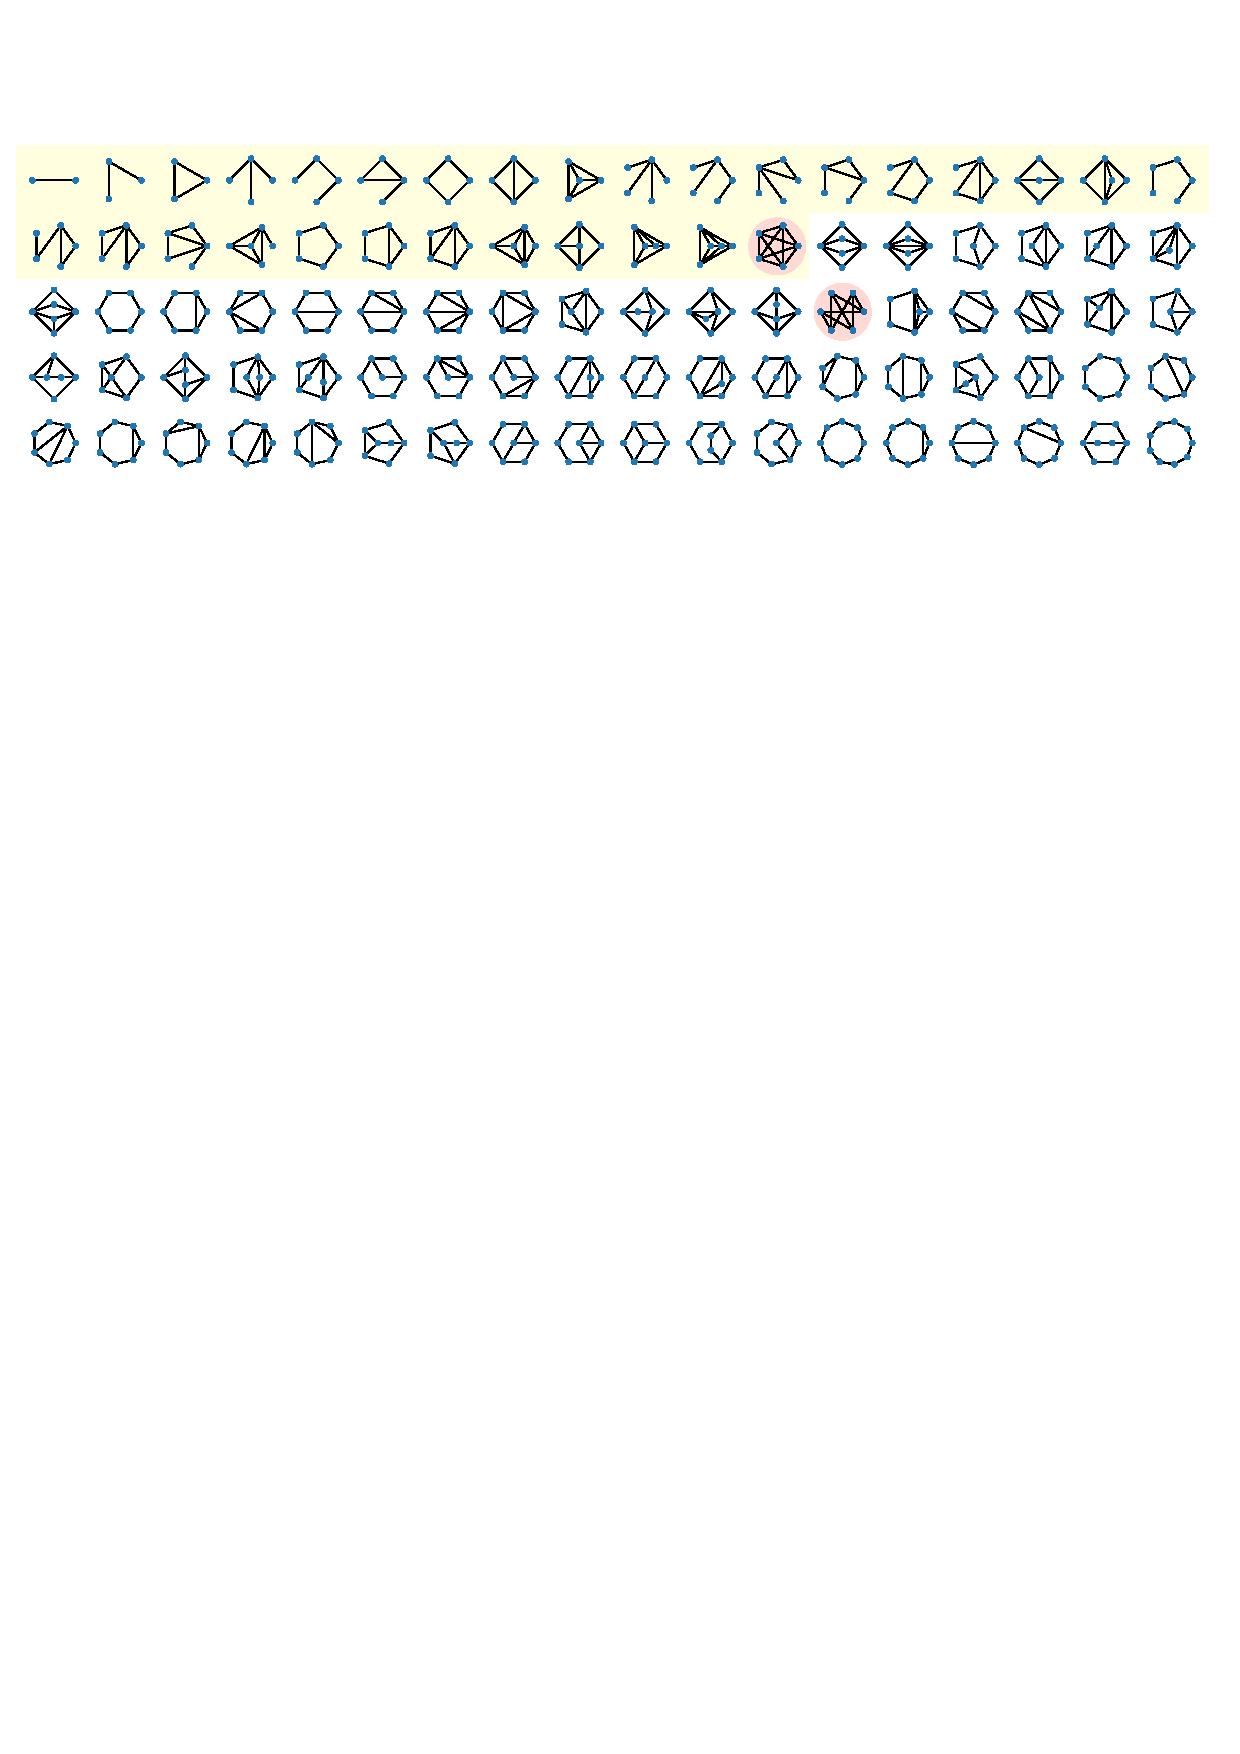
\includegraphics[width=1.0\textwidth]{figures/simple_graphs2.pdf}

\vspace{0.5\intextsep}

$k$-連結性および、極小非平面的グラフは$2$-連結(\cref{lemma:2-connected})は、
それぞれ
第\ref{subsec:tutte}節および第\ref{subsec:kuratowski}節で扱う。
%クラトフスキー\cref{thm:kuratowski}を自明にみえるが、
%本レポートで扱う証明では最小辺数を論拠とする箇所があるため愚直な手続きをとる。



%%%%%%%%%%%%%%%%%%%%%%%%%%%%%%%%%%%%%%%%%%%%%%%%%%%%%%%%%%%%%%%%%%%%%%%%%%%%%%%%%%%%%%%
\subsection{タットの平面描画}\label{subsec:tutte}

ここではタットの平面描画について考察する。
タットの平面描画は1963年にイギリスの数学者タットによって提案された
グラフの描画方法で、平面描画の基礎としての重要な役割を持つ。


\begin{definition}[タットの平面描画]
\label{def:tutte_drawing}
単純で$3$-連結な平面的グラフに対して、
次の三つの制約を満たす描画をタットの平面描画と呼ぶ。
外面境界は凸多角形。
内部の頂点は隣接頂点の重心。各辺は直線分。
\end{definition}


\setcolumnwidth{0.55\textwidth, 0.45\textwidth}
\begin{paracol}{2}
右にタットの平面描画の例を示す。
左は単位正方形内に一様ランダムに生成した
$50$点の集合$S$に対するドロネー三角形分割であり、
右はそれを幾何学的グラフと見做したタットの平面描画である。
定理の第一制約に従い外面境界に$S$の凸包(赤点)をとっている。
このとき第二(隣接重心)・第三(辺直線分)制約を満たすことが確認できる。

\switchcolumn
%\vspace{-1.\intextsep}
\centering
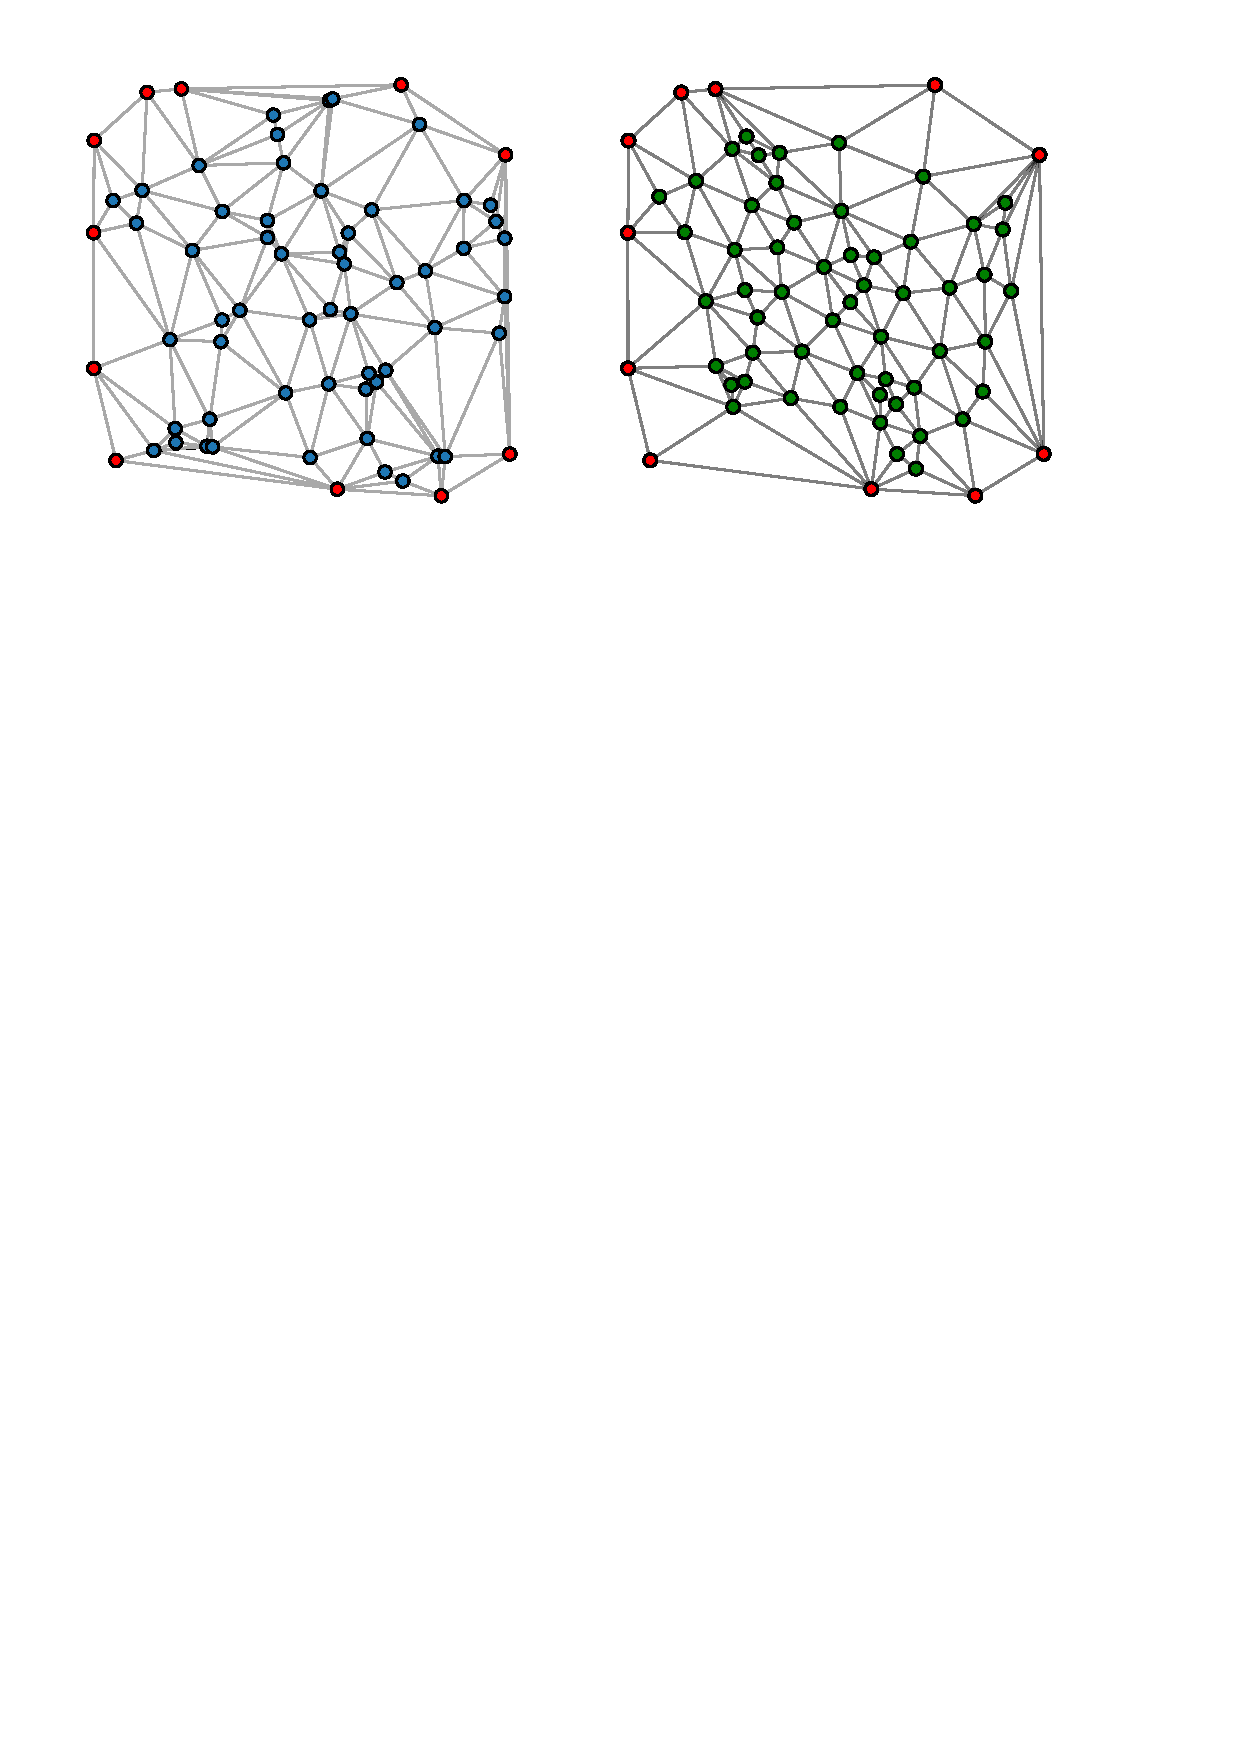
\includegraphics[width=0.4\textwidth]{figures/delaunay_tutte.pdf}
\end{paracol}


\setcolumnwidth{0.85\textwidth, 0.15\textwidth}
\begin{paracol}{2}

\paragraph{$k$-連結性}
\cref{def:tutte_drawing}の前提条件に$3$-連結性が付与されているが、
これは平面描画の縮退を排除するためにある。
連結グラフ$G=(V, E)$の$k$-連結性を任意の整数$k\geq 1$に対して次のように定義する。
どんな$(k-1)$-頂点部分集合$S \subseteq V$を持ってきても
$G \setminus S$が非連結にならないなら$G$は$k$-連結であるという。
また一般的に$k$-連結であれば$(k-1)$-連結である。
右の完全二部グラフ$K_{2,4}$の紫頂点を外面としたタットの平面描画が下段になる。
両端の$2$頂点を削除すると残りは孤立点になるので$K_{2,4}$は$2$-連結グラフである。
このとき外面に属さない頂点は隣接頂点の中点をとるので$2$頂点が一つの座標に収束する。
%これは写像直線分どうしが端点以外の共通部分を持つので平面的ではない。

\switchcolumn
\vspace{1.5\intextsep}
\centering
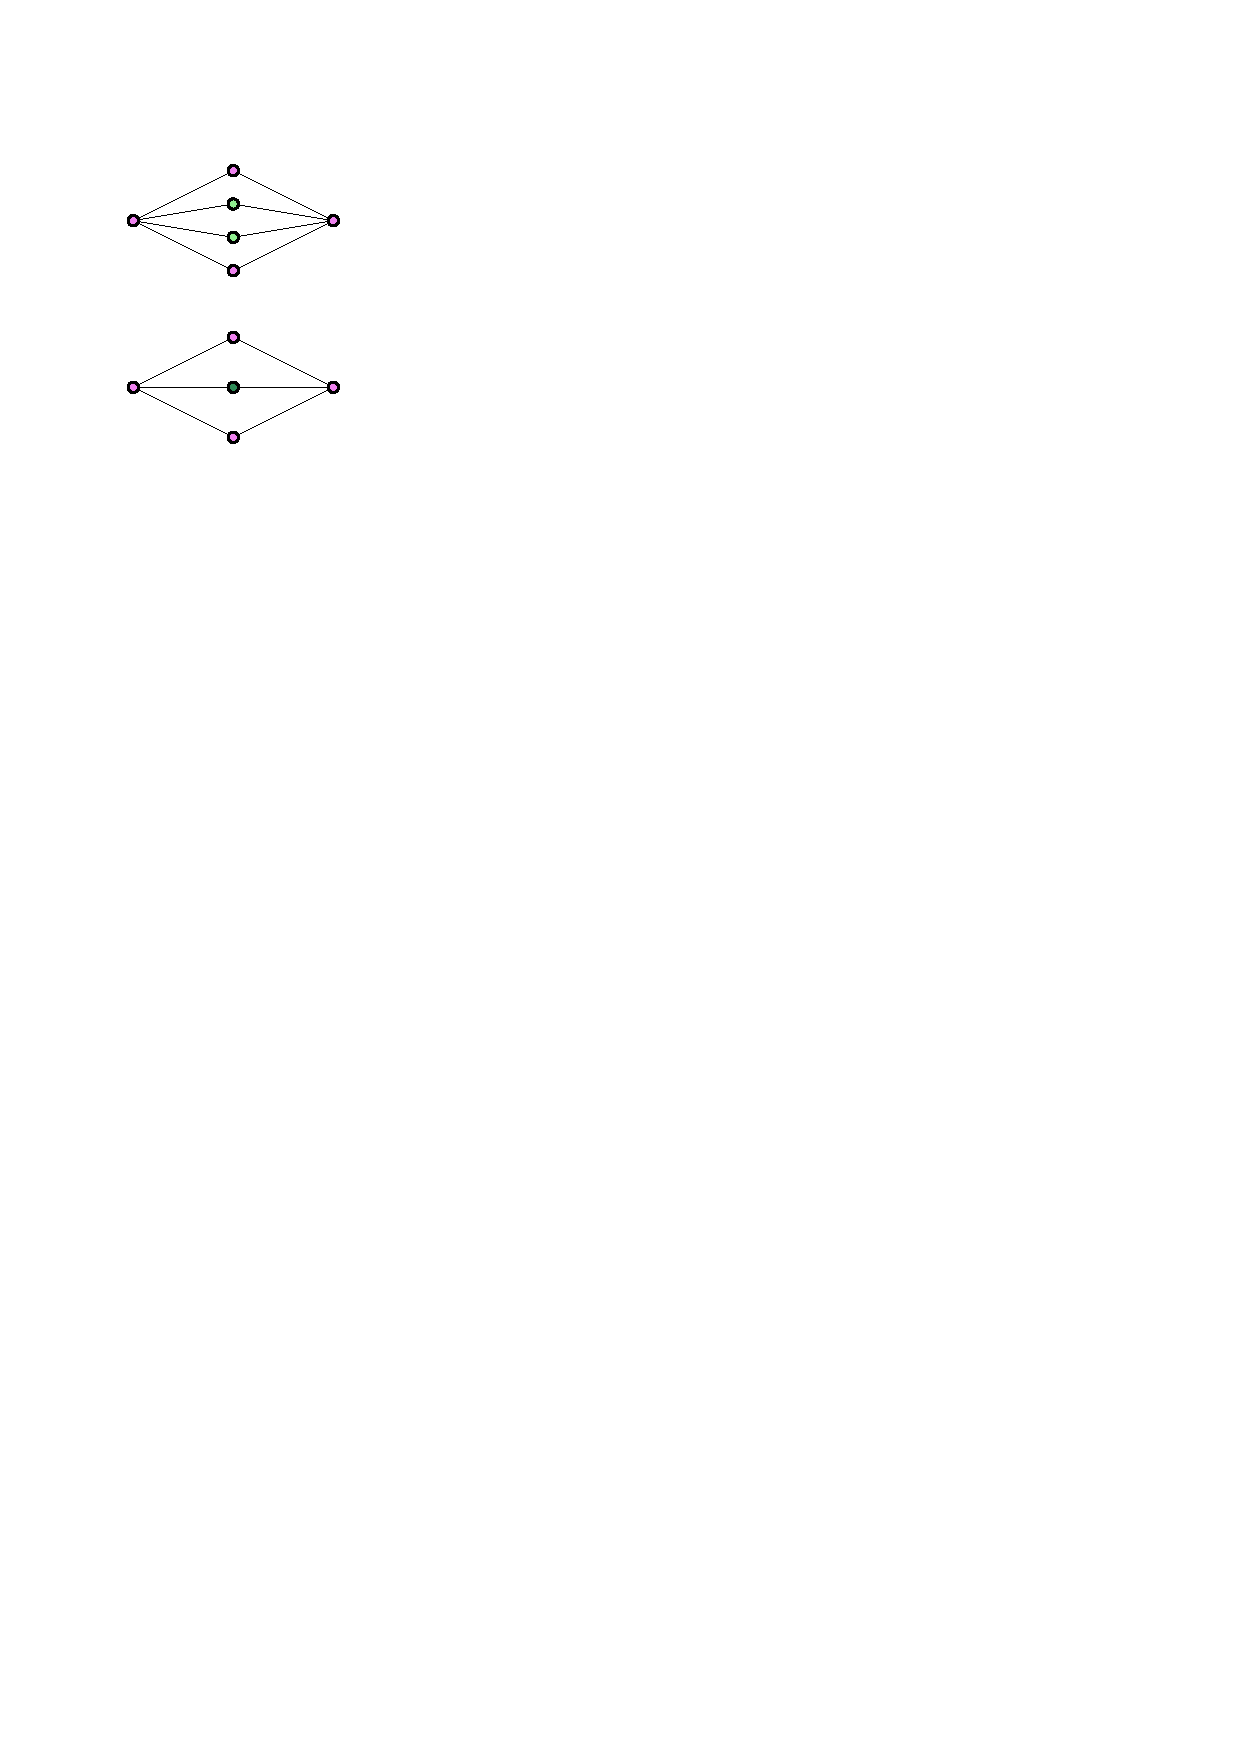
\includegraphics[width=0.12\textwidth]{figures/tutte_degeneracy.pdf}
\end{paracol}


\paragraph{メンガーの定理}
ここで$k$-連結性を特徴付けるメンガーの定理を導入する。
連結性と点素な経路の関係性を記述する非常に使い勝手の良い定理である。
%後述のタットのばね定理およびクラトフスキー定理の証明でも用いている。
二つの$xy$-経路$p_1, p_2$が互いに点素であるとは、
$p_1$と$p_2$の共通頂点が両端点$x,~y$以外に無いことをいう。
%同様に共通する辺を持たない経路対を互いに辺素であるという。
%点素であれば辺素である。

グラフ$G=(V, E)$の頂点集合$A, B \subseteq V$に対して、
頂点集合$S\subseteq V$が$G \setminus S$で$A$から$B$への経路をすべて排除するとき
$S$を$AB$-切断集合という。
$AB$-接続成分を
$A$と$B$を接続し経由頂点が$A \cup B$に属さない経路の集まりから誘導される
$G$の部分グラフとする。
$AB$-接続成分$X$の大きさは$X$に属す$A$と$B$を接続する経路の個数で測られる。

\begin{theorem}[メンガーの定理]
\label{thm:menger}
$G$を連結グラフとし$A, B$を$G$の頂点の部分集合とする。
$G$内のどんな$AB$-切断集合$S$をもってきても$|S| \geq k$なら、
大きさが$k$の$AB$-接続成分$C$が存在する。
\end{theorem}

\setcolumnwidth{0.72\textwidth, 0.28\textwidth}
\begin{paracol}{2}
\begin{proof}
辺の個数に関する構成的な帰納法で示す。
$G$に辺が無いなら$A \cap B$を$C$の頂点集合とすることで主張を満たす。
$G$は$A$から$B$への経路に属す辺$e=(x, y)$を持ち、
$G' = G \setminus e$が大きさ$k$未満の$AB$-切断集合$S$を持つと仮定する。
$P=S\cup\{x\}$および$Q=S\cup\{y\}$はそれぞれ$G$の$AB$-切断集合である。
$|P|=|Q|=|S|+1$。
$G'$の$AP$-切断集合および$QB$-切断集合は、それぞれ
$G$の$AB$-切断集合でもある。
このとき
$G'$は$AP$-接続成分$X$および$QB$-接続成分$Y$を持つ。
$X\cap Y=S$なので$C=(X\cup Y) + e$を得る。
\end{proof}

\switchcolumn
\vspace{0.5\intextsep}
\centering
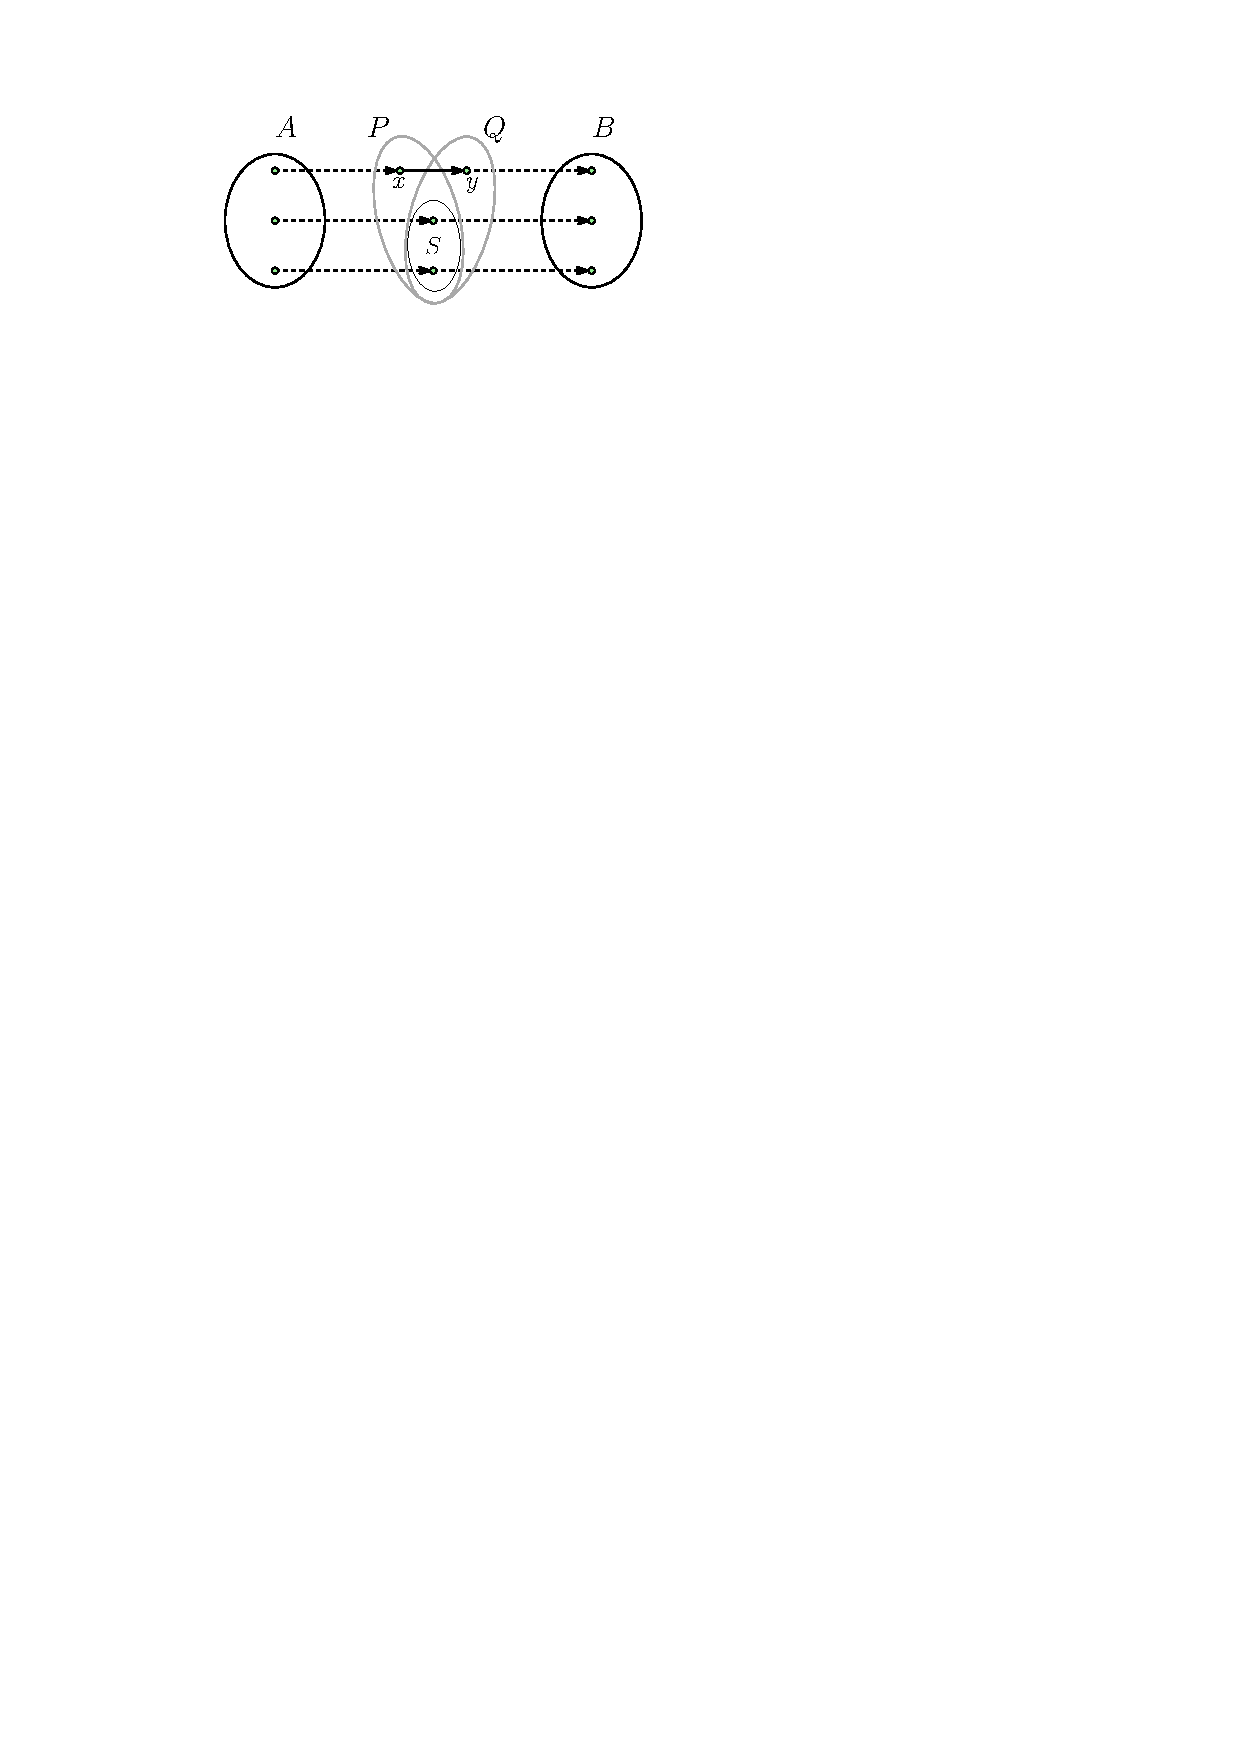
\includegraphics[width=0.27\textwidth]{figures/menger_goring_proof.pdf}
\end{paracol}

$AB$-接続成分$X$に属す$k$個の経路が点素であることは
切断集合に対する$k$の最小性から導ける。
証明の構成からも分かる通り$X$内の経路$p_1, p_2$が共通の経由頂点$v$を持つなら
$v$は$S$に属していなければならず、いずれか一方は冗長であり排除される。
もう少し厳密には以下の系に従う。
$x, y \in V$に対して$S$が次の条件を満たすとき$S$は$x$と$y$を切断するという。
$\{x, y\}\cap S = \varnothing$かつ$x$から$y$へのどんな経路を持ってきても
$S$の頂点を通過する。

\begin{corollary}
\label{coro:pairwise_independent}
$G=(V,E)$を対象グラフとし$s,t\in V$とする。ただし$s \neq t$で$(s, t) \notin E$。
$s$と$t$を切断するどんな集合$S$も$|S|\geq k$なら
非冗長で点素な$st$-経路が$k$個存在する。
\end{corollary}
\begin{proof}
$G'=G\setminus\{s,t\}$および$A=N(s), B=N(t)$とする。
$G'$内のどんな$AB$-切断集合$S$も$G$において$s$と$t$を切断し$|S|\geq k$を満たす。
%そのサイズは少なくとも$k$はある。
メンガーの\cref{thm:menger}より
大きさ$k$の$AB$-接続成分$X$が存在する。
始点として$s$から$A$の各頂点に接続し、
終点として$B$の各頂点から$t$に接続することで$k$個の点素な$st$-経路を得る。
\end{proof}






\paragraph{タットの平面描画の求め方}
$n$-頂点グラフ$G=(V,E)$のタットの平面描画$\Gamma$は、
$xy$-座標それぞれ$n$個の一次式からなる2つの連立方程式を解くことで得られる。
$\Gamma$は任意の$v\in V$に対して
$v$を$\Gamma(v)=(x_v^*, y_v^*) \in \mathbb{R}^2$へ写像する。
外面境界上の頂点集合を$F \subseteq V$とする。
$F$の頂点$v$は凸の位置に固定されるので
一次式$x_v = x_v^*,~ y_v=y_v^*$を得る。
%$F$内の頂点は凸の位置に固定されるので一次式は
%$x_v = x_v^*$および$y_v=y_v^*$となる。
$V \setminus F$内の頂点に関しては
一次式$\deg(v)\cdot x_v - \sum_{w \in N(v)} x_w = 0$および
$\deg(v)\cdot y_v - \sum_{w \in N(v)} y_w = 0$として
隣接頂点の重心に座標値をとる制約として定式化する。


具体的なpythonコードは下記の\lstrefname\ref{lst:tutte}のように書ける。
この例では numpy パッケージを用いる。
\begin{lstlisting}[language=Python, caption=タットの平面描画,label=lst:tutte]
def tutte_embedding(G, F, pos):
    A, Bx, By = [], [], []
    for u in g:
        a, bx, by = [0] * G.number_of_nodes(), 0, 0
        if u in F:
            a[u] = 1
            bx, by = pos[u]
        else:
            a[u] = len(G.neighbors(u))
            for v in G.neighbors(u):
                a[v] = -1
        A.append(a)
        Bx.append(bx)
        By.append(by)
    xcoords = np.linalg.solve(A, Bx)
    ycoords = np.linalg.solve(A, By)
    return {i: (x, y) for i, (x, y) in enumerate(zip(xcoords, ycoords))}
\end{lstlisting}
入力は、対象グラフ{\tt G}と外面境界上の頂点部分集合の{\tt list F}、
{\tt F}内の各頂点の座標情報の{\tt dict pos}。
{\tt G}の頂点は整数識別子で管理されているものとする。
このとき、
連立一次方程式を定義するために係数行列{\tt A}と係数ベクトル{\tt Bx, By}を導入し(第2行)、
制約条件に基づき適宜係数を構成していく(第3-14行)。
そして第15・16行で連立一次方程式ソルバ
{\tt numpy.linalg.solve}を用いて具体的な座標を得る。
最後に頂点から座標値への単射としての連想配列を形成し出力する(第17行)。


\setcolumnwidth{0.75\textwidth, 0.25\textwidth}
\begin{paracol}{2}

\paragraph{包囲閉路}
与えられた$3$-連結な平面的グラフ$G$に対して
正しくタットの平面描画を得るには、
外面境界上の頂点系列を適切に取得する必要がある。
平面埋込みが与えられていれば任意の面を外面として選択%し、
%外面境界上の頂点を自己交差しない凸の位置に配置
すれば適切に平面描画が得られる。
別の言い方をすると、外面境界は包囲閉路であれば平面描画となる。

\switchcolumn
%\vspace{1.5\intextsep}
\centering
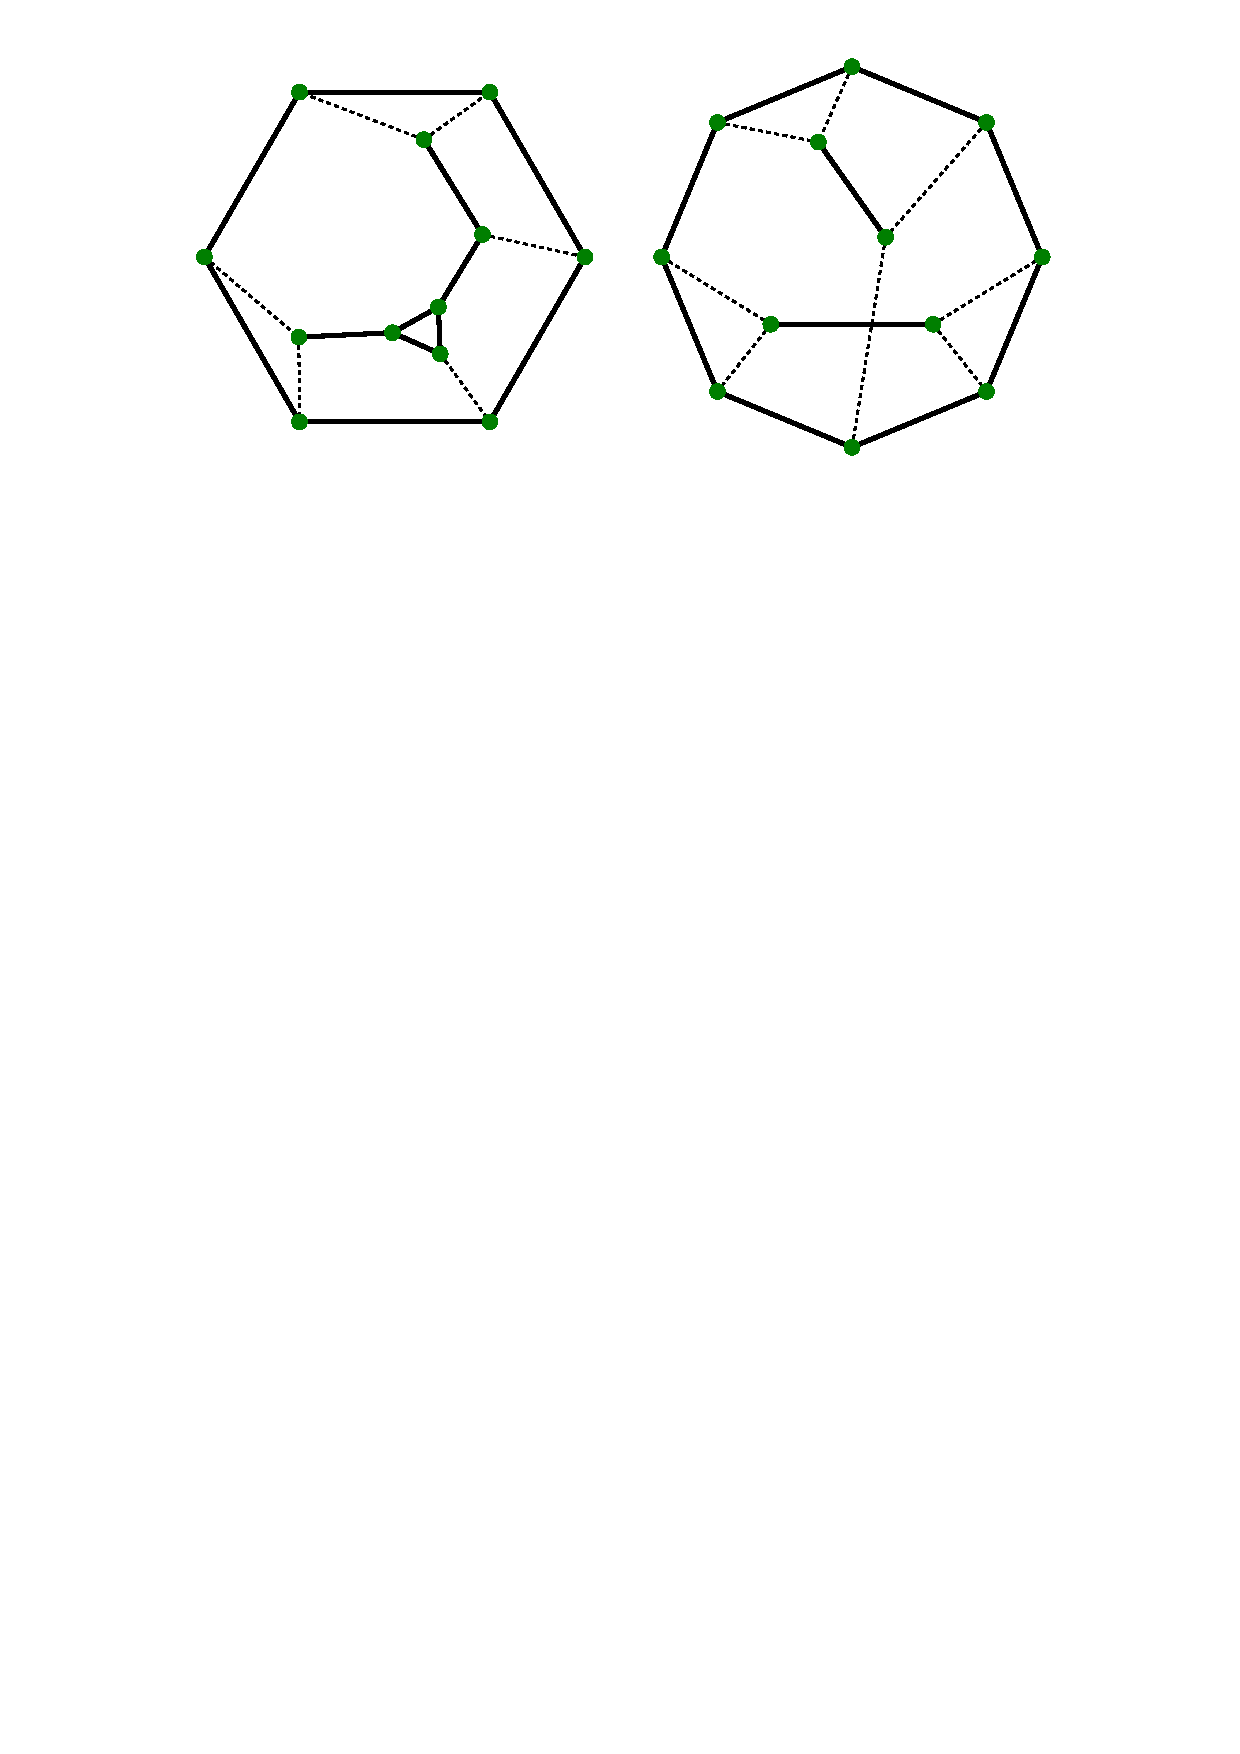
\includegraphics[width=0.24\textwidth]{figures/tutte_frucht_error.pdf}
\end{paracol}
包囲閉路$C$は、
$G\setminus C$が連結で、$C$内で隣接しない頂点間を接続する辺を$E$内に持たない閉路である。
包囲閉路の第二制約は$K_4$の4頂点を外面と選んだ時に対角線どうしが
交差すること排除するための制約である。
右上はフルフトグラフの異なる外面選択時のタットの平面描画を示している。
左は包囲閉路だが右は違う。そのため交差する辺対を持つ。




\paragraph{平面上の右と左}

平面上の$3$点$p_i=(x_i, y_i) \in \mathbb{R}^2,\ i=1, 2, 3$に対して、
向き$\orient(p_1, p_2, p_3)$を次のように行列式を用いて定義する。
\setcolumnwidth{0.85\textwidth, 0.15\textwidth}
\begin{paracol}{2}
\vspace{-1.5\intextsep}
%\[
\begin{align*}
\orient(p_1, p_2, p_3) =
    \left|
        \begin{array}{ccc}
            x_1 & y_1 & 1 \\
            x_2 & y_2 & 1 \\
            x_3 & y_3 & 1
    \end{array}
    \right| &=
    \left|
        \begin{array}{cc}
            x_1 - x_3 & y_1 - y_3 \\
            x_2 - x_3 & y_2 - y_3
        \end{array}
    \right| \\
&=(x_1 - x_3)(y_2 - y_3) - (x_2 - x_3)(y_1 - y_3).
\end{align*}
%\]
\switchcolumn
%\vspace*{1.5\intextsep}
\centering
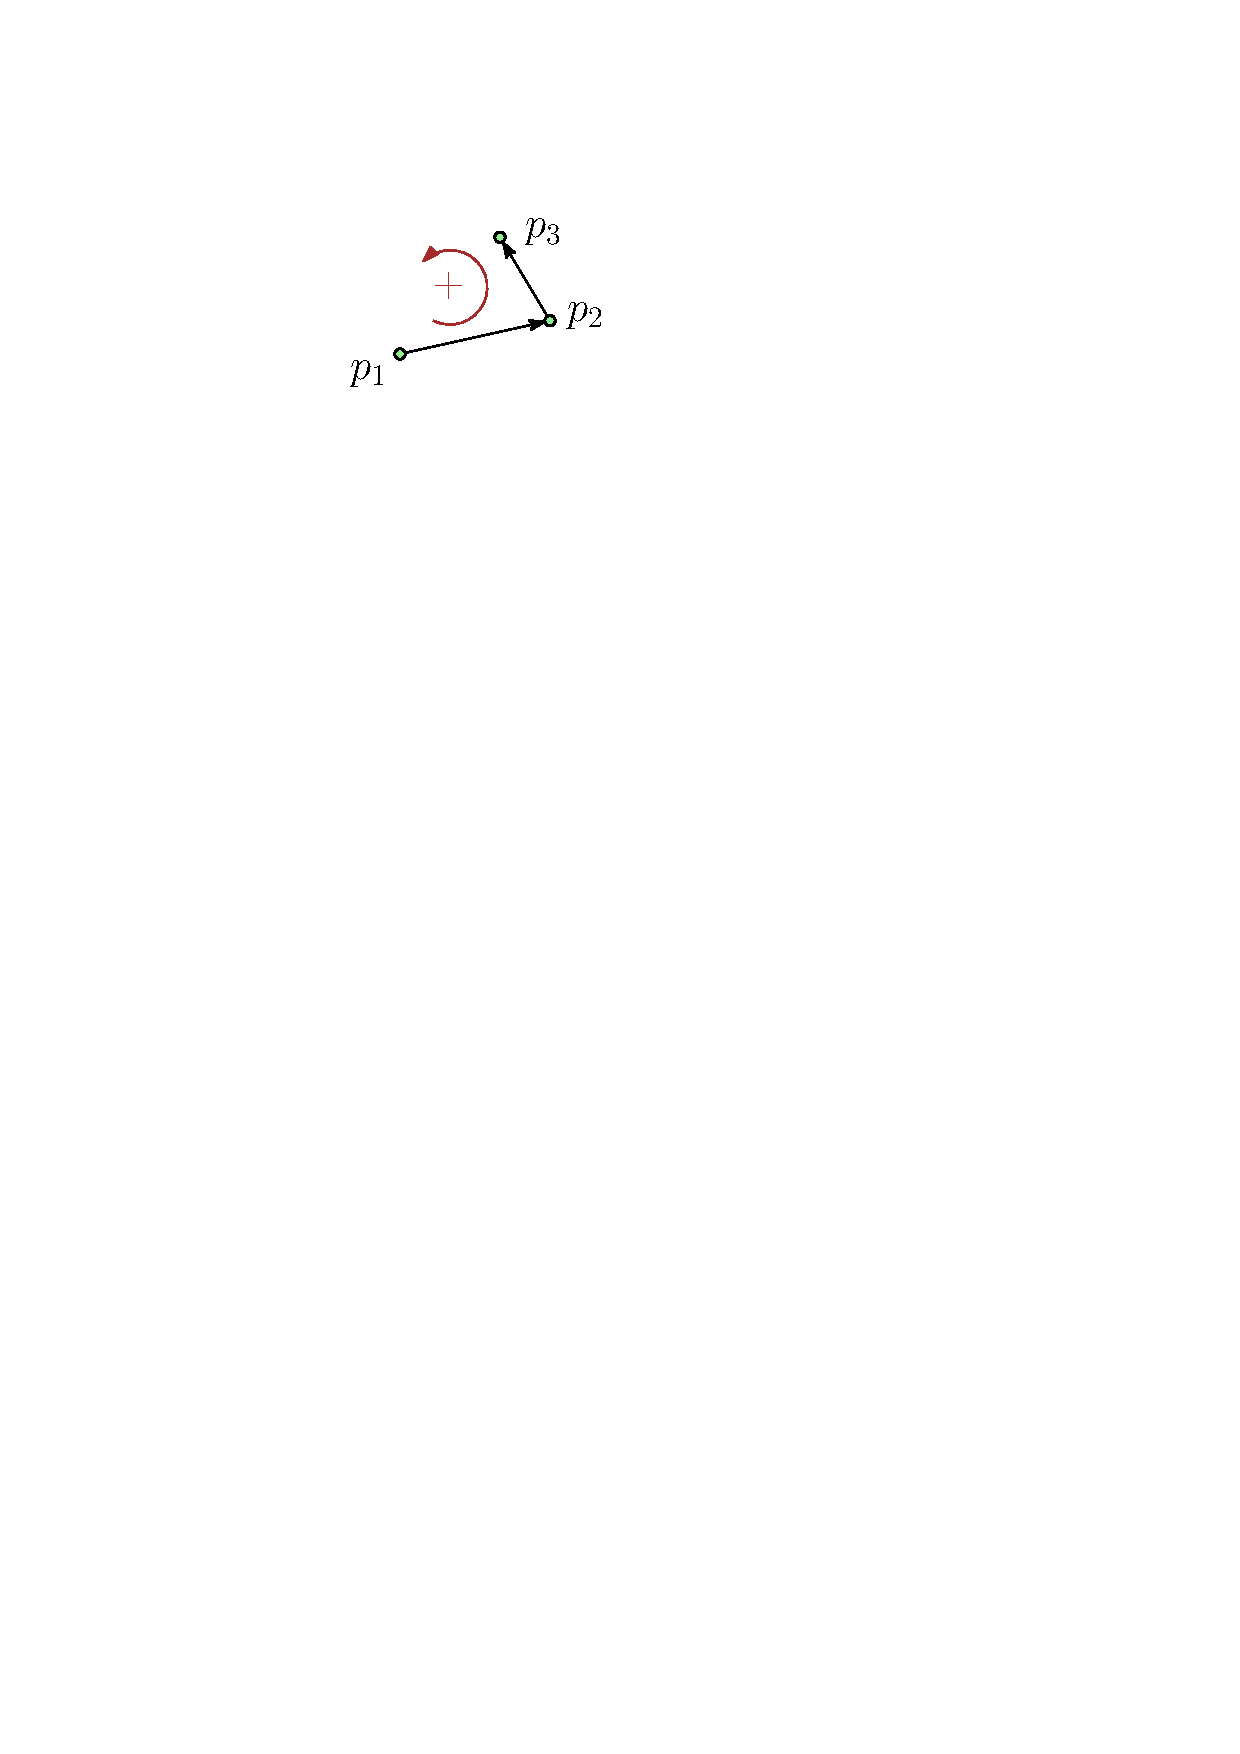
\includegraphics[width=0.13\textwidth]{figures/orientation.pdf}
\end{paracol}
向き$\orient$は三角形の符号付き面積の外積計算そのものである。
従って$\orient$の値が大きいほど$p_3$から$p_1, p_2$を通る直線への垂直距離は大きくなる。
$\orient(p_1, p_2, p_3) = 0$のとき三点は同一直線上にある。
また、$\orient(p_1, p_2, p_3) < 0~(> 0)$のとき右(左)回りもしくは(反)時計回りであり、
$p_3$は$p_1, p_2$を通る直線の右(左)にあるという。
上図は$\orient(p_1, p_2, p_3) > 0$の例を示している。
%おり、($p_1, p_2, p_3)$は反時計回りであり、
%$p_3$は$p_1, p_2$を通る直線の左にある。
%同様に$\orient(p_1, p_2, p_3) < 0$なら$p_3$は右にあるという。





%%%%%%%%%%%%%%%%%%%%%%%%%%%%%%%%%%%%%%%%%%%%%%%%%%%%%%%%%%%%%%%%%%%%%%%%%%%%%%%
\paragraph{タットの平面描画の平面性保証}
タットの平面描画の三制約(外面凸多角形・隣接重心・辺直線分)を満たす描画は、
正しく平面描画になることを示す。
具体的には任意の辺対の写像が交差しないことを議論する。
\begin{theorem}[タットのばね定理]
\label{thm:tutte}
$3$-連結な平面的グラフに対する任意のタットの平面描画は、
どの辺対の写像も交差しない。
\end{theorem}




%%%%%%%%%%%%%%%%%%%%%%%%%%%%%%%%%%%%%%%%%%%%%%%%%%%%%%%%%%%%  Tutte spring theorem.

\begin{proof}%[Proof of \cref{thm:tutte}.]
$p\in \mathbb{R}^2$が
$G$のどの辺の写像にも属さないときファセット上の点と呼ぶ。
ファセット上の点$p$はどれも唯一の面に属すことを示し、
辺対の写像が交差するならその交点の近傍で矛盾が生じることを導く。
外面境界の外部に$p$が属すなら、
タットの平面描画の三つの3制約は外面以外の面に属さないことを保証する。
内部の$p$に対しては
頂点や辺の写像と交差しない半径$\varepsilon ~> 0$の円が描ける。
\cref{lemma:tutte_opposite}より、
任意の辺$e$を共有する二つの面は$e$の写像直線分の左右に分かれるので$p$は唯一の面に属す。
%
%このとき、タットの平面描画の任意の辺対の写像どうしが交差すると仮定すると、
%その交点付近のファセット上の点は二つの面に属すことになり矛盾。
\end{proof}




%%%%%%%%%%%%%%%%%%%%%%%%%%%%%%%%%%%%%%%%%%%%%%%%%%%%%%%%%%%%%%%%%%%%%%% Tutte opposite
\begin{lemma}
\label{lemma:tutte_opposite}
$G=(V, E)$を$3$-連結な平面的グラフ、$\Gamma$を$G$のタットの平面描画とする。
$\ell$を境界上に無い辺$(u, v) \in E$の
端点の写像$p_1=\Gamma(u), p_2=\Gamma(v)$を通る直線とする。
$S_1,~ S_2$をそれぞれ$(u, v)$を共有する二つの面の境界上の$u, v$を除く頂点の集合とする。
%$S_0, S_1$をそれぞれ$F_0, F_1$を構成する$u, v$以外の頂点からなる集合とする。
このとき、$S_1$と$S_2$内の頂点の写像はそれぞれ$\ell$の左右に分かれて存在する。
\end{lemma}

\setcolumnwidth{0.75\textwidth, 0.25\textwidth}
\begin{paracol}{2}
\begin{proof}
$S_1$と$S_2$が$\ell$上か$\ell$の右に存在する
頂点$s_1 \in S_1,~ s_2 \in S_2$をそれぞれ持つと仮定する。
つまり$\orient(p_1, p_2, \Gamma(s_1)) \leq 0$および
$\orient(p_1, p_2, \Gamma(s_2)) \leq 0$。


\cref{lemma:tutte_collinear}および\cref{lemma:tutte_left_right}より、
$s_1,~ s_2$は共に$\ell$の右に写像される隣接頂点を持つ。
\cref{lemma:tutte_connected}より、
経由する頂点がすべて$\ell$の右に写像される$s_1 s_2$-経路$P$が存在する。
%$u,~v$についても同様に、
同様に$u$と$v$はいずれも$\ell$の左に隣接頂点を持ち、
経由する頂点がすべて$\ell$の左に写像される$uv$-経路$Q$が存在する。
\cref{lemma:tutte_left_right}より$Q$は$(u, v)$でない。
また$P$と$Q$は互いに点素。
これは\cref{lemma:tutte_cycle_intersection}に矛盾する。
\end{proof}
\switchcolumn
%\vspace{1.5\intextsep}
\centering
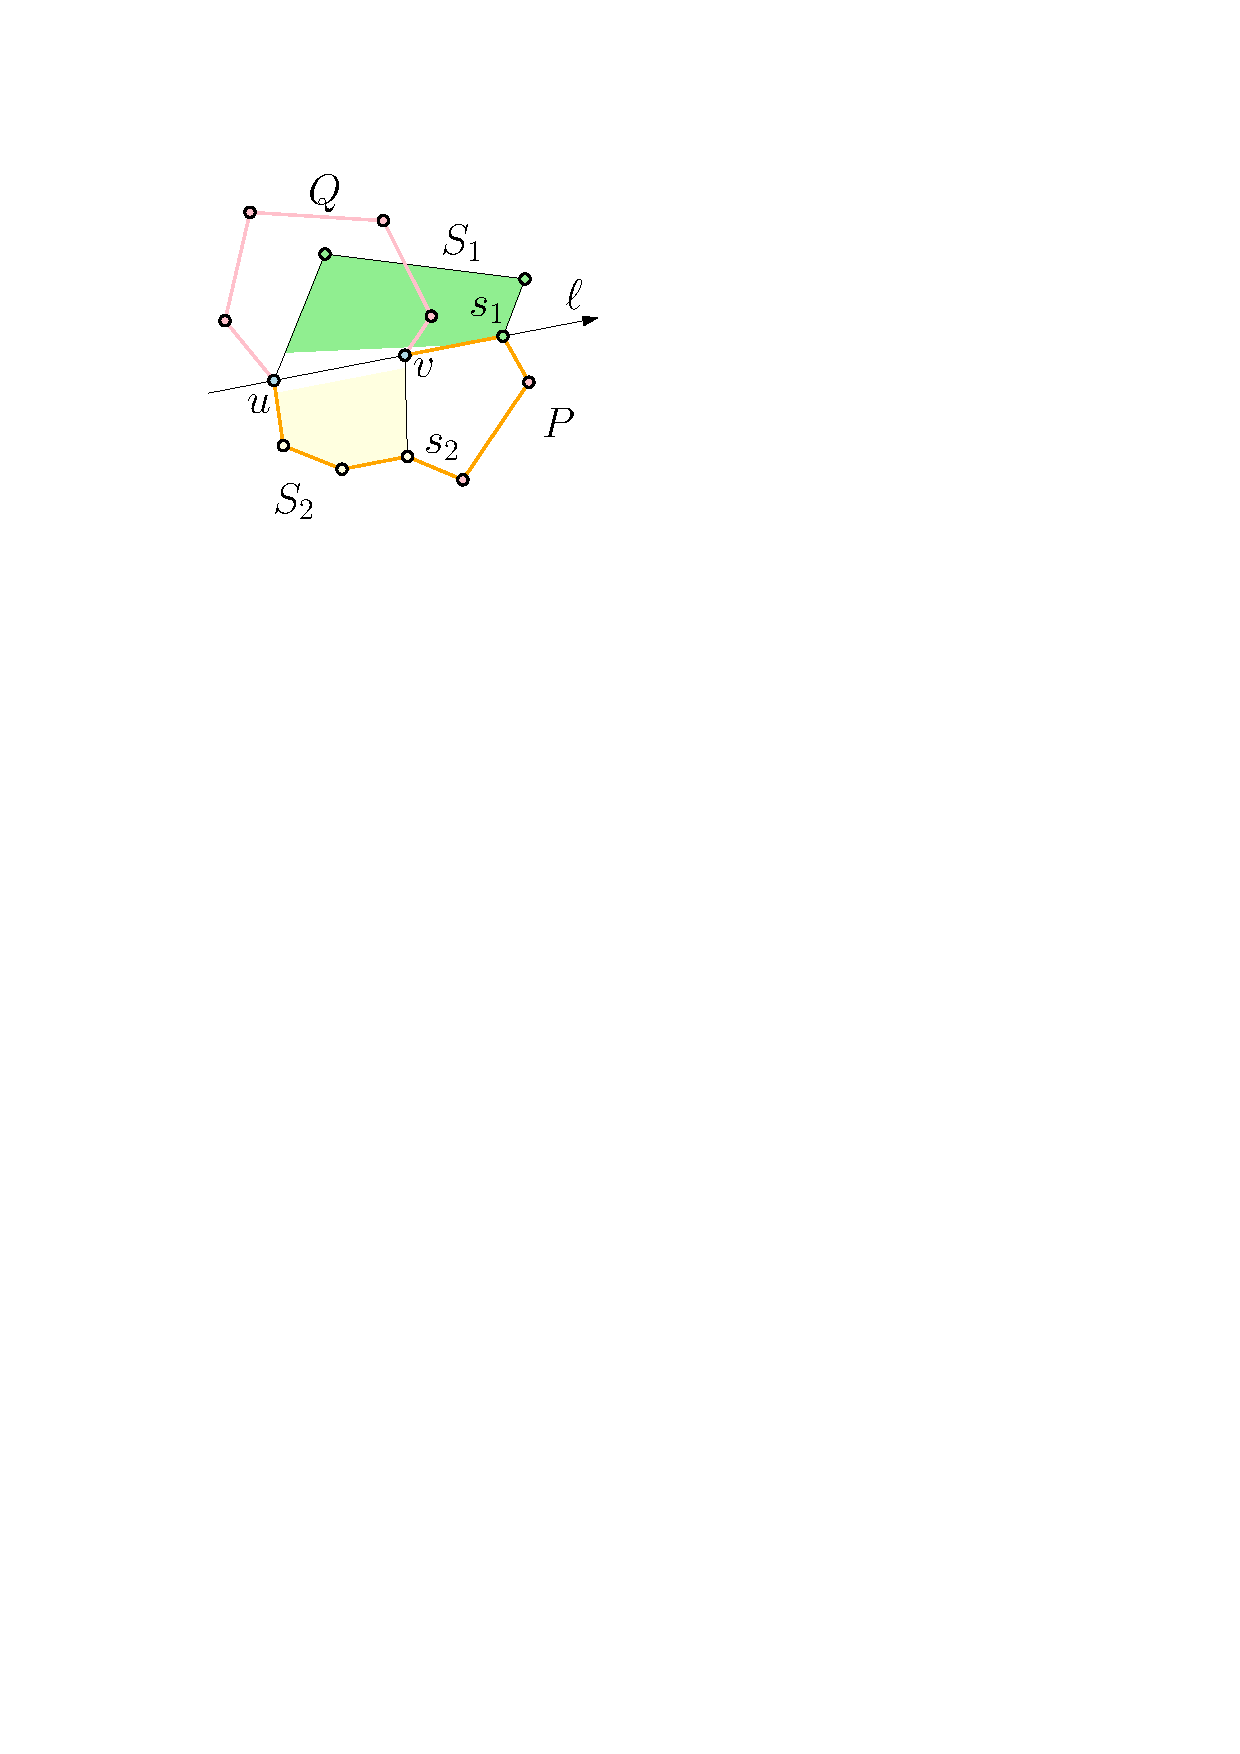
\includegraphics[width=0.2\textwidth]{figures/tutte_opposite.pdf}
\end{paracol}





%%%%%%%%%%%%%%%%%%%%%%%%%%%%%%%%%%%%%%%%%%%%%%%%%%%%%%%%%%%%%%%%%%%%%%% Tutte collinear
\begin{lemma}
\label{lemma:tutte_collinear}
隣接頂点すべての写像が同一直線上に配置される頂点は存在しない。
\end{lemma}

\setcolumnwidth{0.75\textwidth, 0.25\textwidth}
\begin{paracol}{2}
\begin{proof}
%外面境界上の頂点集合$F$に関しては前提条件。
すべての隣接頂点が直線$\ell$上に位置する頂点$v$が存在すると仮定する。
$S^+,~ S^-$をそれぞれ$\ell$の左と右に写像を持つ頂点の集合とする。
$U$を$v$から到達可能な頂点$u$で$N(u)$がすべて$\ell$上に写像される頂点集合とする。
少なくとも$v \in U$。
$W$を$v$から到達可能で$\ell$上に写像されるが$S^+,~ S^-$に隣接頂点を持つ頂点の集合とする。
\cref{lemma:tutte_left_right}より$W\neq \varnothing$。
また、対象グラフは$3$-連結であり、
$W$は$U$と$S^+\cup S^-$に対する切断集合なので$|W|\geq 3$。
%$W$の各頂点は$S^+$と$S^-$両方に隣接頂点を持つ。
\cref{lemma:tutte_connected}より$S^+$と$S^-$はそれぞれ連結である。
$w_1, w_2, w_3 \in W$および$S^+, U, S^-$は$K_{3,3}$の細分を形成する。
\end{proof}
\switchcolumn
\vspace{-1.5\intextsep}
\centering
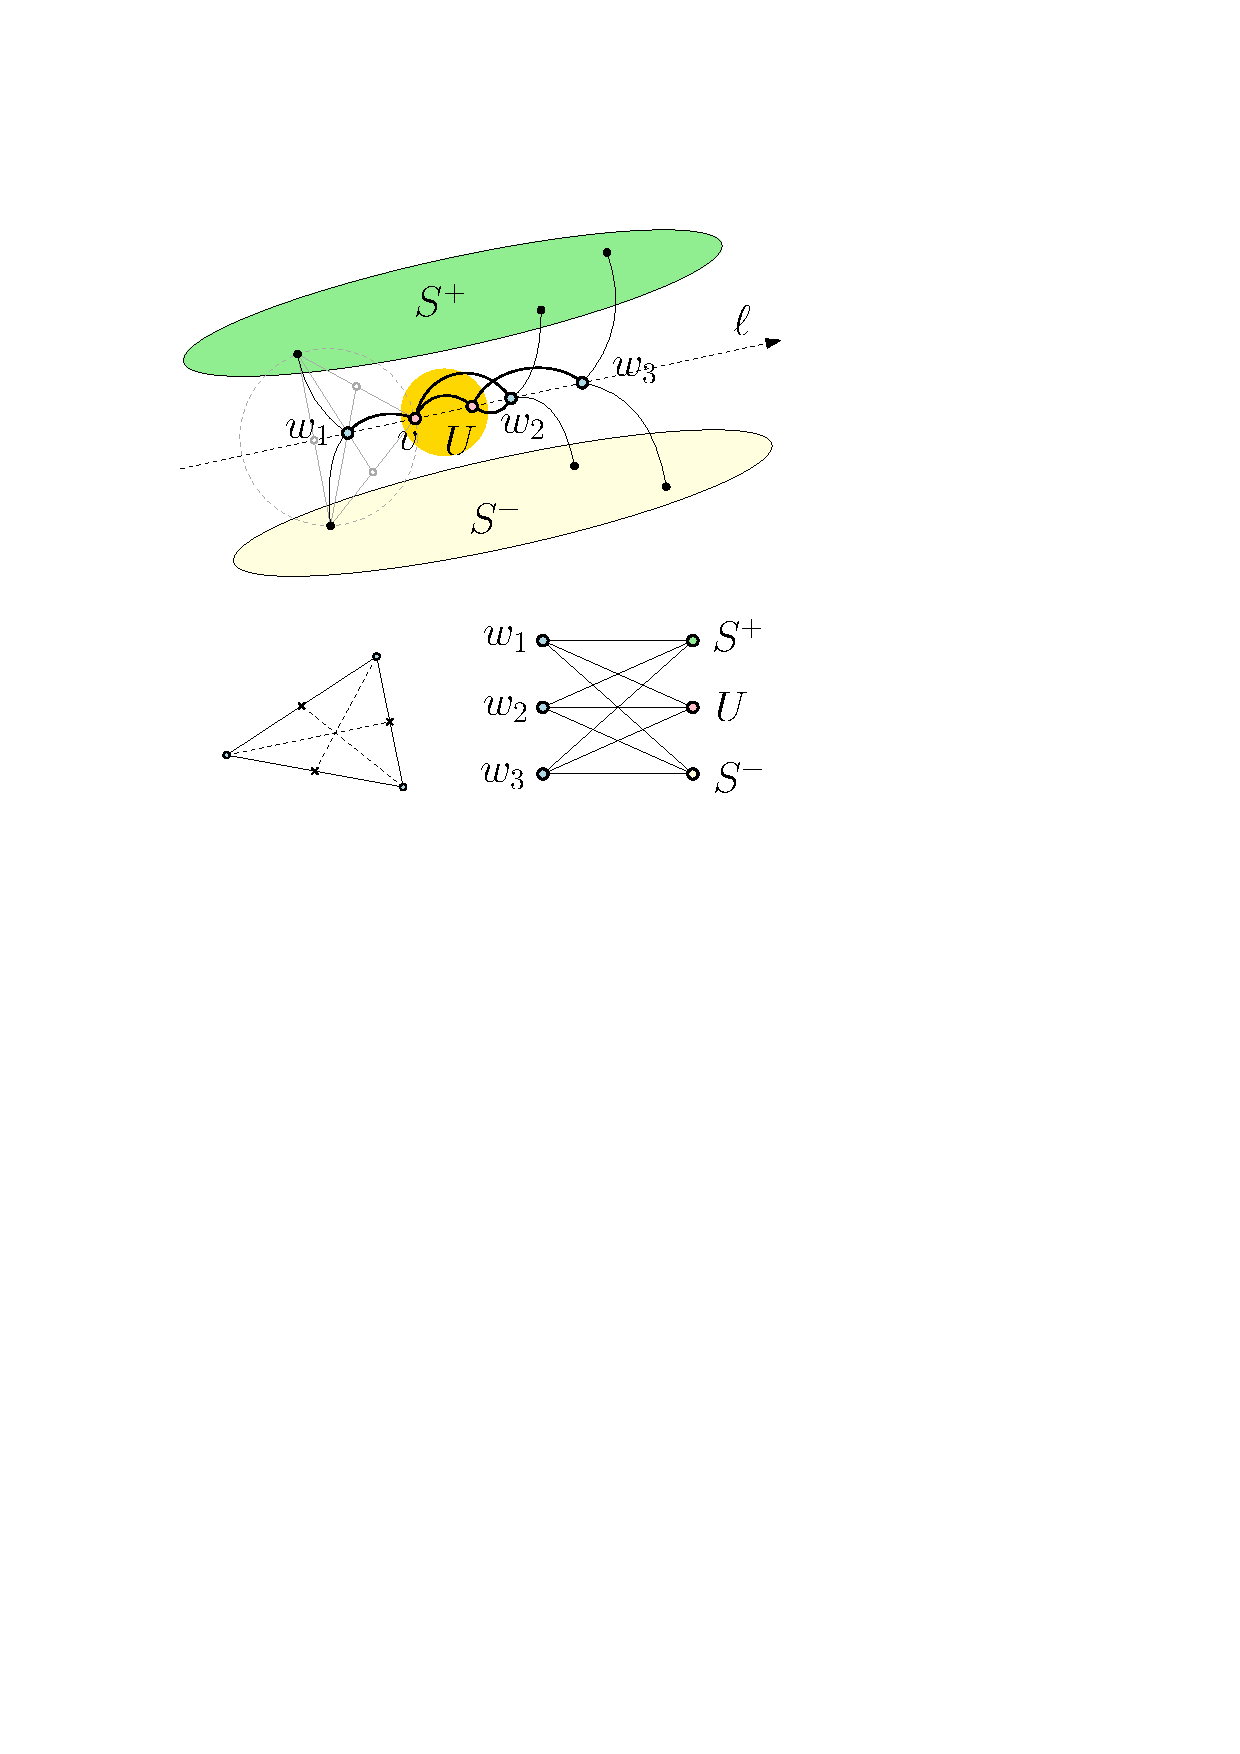
\includegraphics[width=0.24\textwidth]{figures/tutte_collinear.pdf}
\end{paracol}










\begin{lemma}
\label{lemma:tutte_left_right}
$\ell$をある頂点$v \in V$の写像$p_1 = \Gamma(v)$と
任意の点$p_2 \in \mathbb{R}^2$を通る直線とする。
$\ell$の左に位置する$v$の隣接頂点が非空
$\{u \in N(v) ~|~ \orient(p_1, p_2, \Gamma(u)) > 0\} \neq \varnothing$なら
右の隣接頂点も非空$\{u \in N(v) ~|~ \orient(p_1, p_2, \Gamma(u)) < 0\} \neq \varnothing$。
\end{lemma}

\begin{proof}
任意の内部頂点は、
第2制約により各$xy$-座標の平均値をとるので、
隣接頂点の写像が形成する凸包の外部に位置することはない。
\end{proof}


%%%%%%%%%%%%%%%%%%%%%%%%%%%%%%%%%%%%%%%%%%%%%%%%%%%%%%%%%%%%%%%%%%%%%%%%%%コメントアウト
\begin{comment}
\begin{lemma}
外面境界上の頂点集合$F$に無いすべての頂点は$F$の凸包内部$C$に含まれる。
\end{lemma}

\begin{proof}
外面境界上の点集合の任意の$3$点$v_1, v_2, v_3$からなる集合を$A$、$B=\{v\}$とするとき
メンガーの\cref{thm:menger}より$v$から$v_i,~ i=1,2,3$への点素経路を持つ。
$\Gamma(v)$は$\Gamma(v_i), i=1,2,3$の加重平均と見做せるので
$C$の境界上ではない内部に配置される。
\end{proof}
\end{comment}
%%%%%%%%%%%%%%%%%%%%%%%%%%%%%%%%%%%%%%%%%%%%%%%%%%%%%%%%%%%%%%%%%%%%%%%%%%コメントアウト



\begin{lemma}
\label{lemma:tutte_connected}
$G=(V,E)$を対象のグラフ、$\Gamma$を任意のタットの平面描画、
$H$を任意の$2$点$p_1, p_2 \in \mathbb{R}^2,~ p_1\neq p_2$を通る直線で区切られる
半平面$\{p \in \mathbb{R}^2 ~|~ \orient(p_1, p_2, p) > 0\}$とする。
%このとき
$S = \{v \in V~|~ \Gamma(v)\in H\}$が誘導する部分グラフ$G[S]$は連結。
\end{lemma}

\vspace*{-0.5\intextsep}
\setcolumnwidth{0.78\textwidth, 0.22\textwidth}
\begin{paracol}{2}
\begin{proof}
平面上の点$p\in \mathbb{R}^2$に対して$\tau(p) = \orient(p_1, p_2, p)$とおく。
$F$を外面境界上の頂点集合とする。
$H$の境界線から最も離れた頂点$t = \argmax_{v\in V}\tau(\Gamma(v))$は$t\in F$。
任意の頂点$s\in S$から$t$への経路$s=v_0, v_1, \ldots, v_k=t$で
連続する二頂点$v_i, v_{i+1}$が
$\tau(\Gamma(v_i)) \leq \tau(\Gamma(v_{i+1}))$ を満たす経路が存在することを示す。

$p=\Gamma(s),~ q=\Gamma(t)$とおく。
$\tau(p) = \tau(q)$のとき
$s$と$t$はいずれも$F$内の頂点で互いに隣接する。
%これは$p_1, p_2$および$p, q$それぞれの方向ベクトルが平行で、すなわち
%符号付き面積が等しくなることを意味する。
%
$\tau(p) < \tau(q)$のとき二つの場合を考える。
%$s$から$t$への$\tau$が非減少の経路が存在することを示す。
$s \in F$なら外面境界を辿り$t$へ到達する経路が存在する。
$s \notin F$なら\cref{lemma:tutte_left_right}より、
$\tau(p) < \tau(\Gamma(v))$を満たす$v \in N(s)$が存在する。
これは帰納的に成り立ち、$S$の任意の頂点は$t$へ到達可能。
\end{proof}
\switchcolumn
\vspace{1.5\intextsep}
\centering
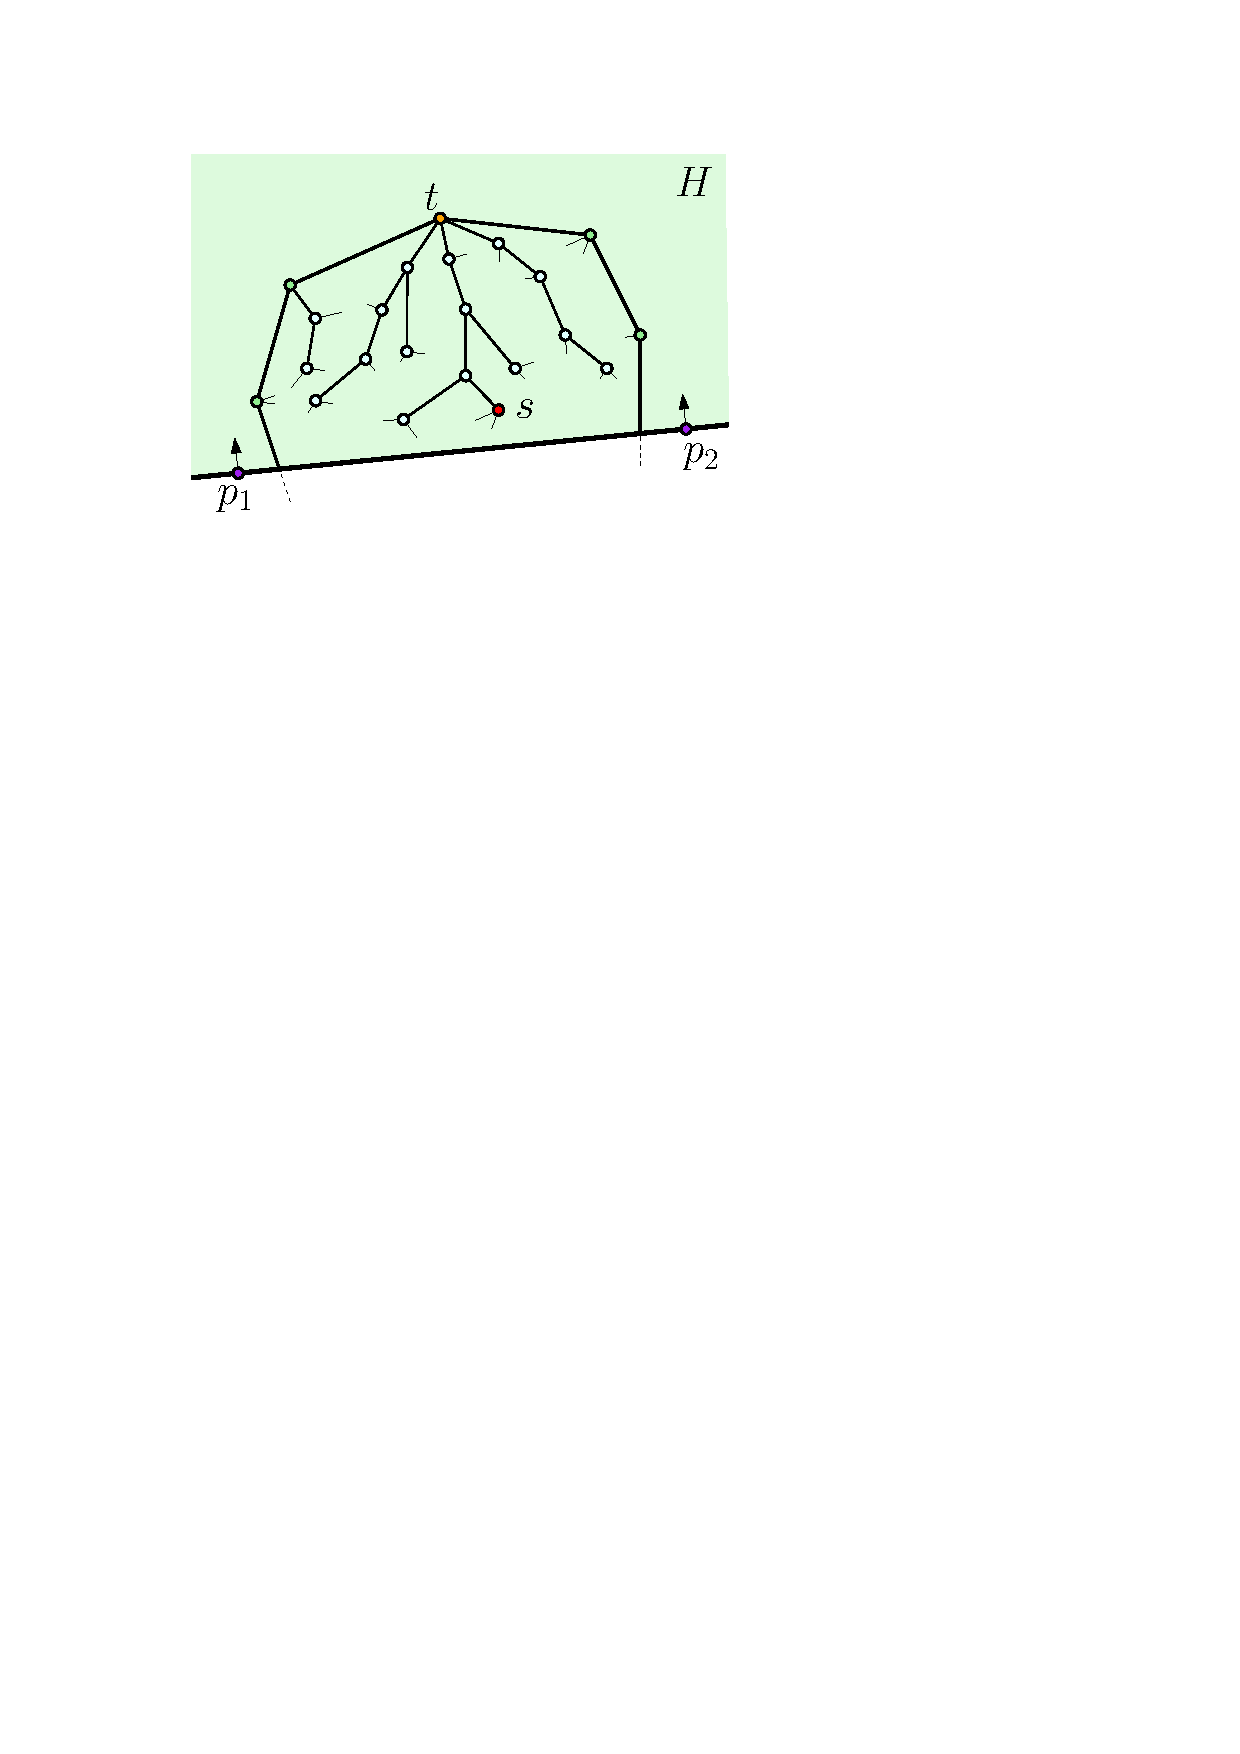
\includegraphics[width=0.21\textwidth]{figures/tutte_connected.pdf}
\end{paracol}




\setcolumnwidth{0.75\textwidth, 0.25\textwidth}
\begin{paracol}{2}
\begin{lemma}
\label{lemma:tutte_cycle_intersection}
$G$を$3$-連結な平面的グラフ、$(u, v)$を$G$の任意の辺とする。
$S_1, S_2$をそれぞれ$(u, v)$を共有する面の$u, v$を除く頂点集合とする。
$P$をその端点が$s_1 \in S_1,~ s_2 \in S_2$で$u, v$を経由しない$G$上の経路とする。
このとき、$G$上の任意の$uv$-経路は$P$と共通頂点を持つか$(u, v)$自身である。
\end{lemma}


\begin{proof}
$G$の任意の平面描画を考える。
このとき$P$と$s_1, s_2$を仮想的につなげたジョルダン閉曲線$C$が描ける。
$C$の仮想的な部分曲線は$(u, v)$の写像とだけ交差し、$u$と$v$を内と外に分かつ。
従って、$u$と$v$を端点とするどんな経路も$P$と少なくとも一つの頂点を共有するか
辺$(u, v)$そのものである。
\end{proof}
\switchcolumn
\vspace{1.\intextsep}
\centering
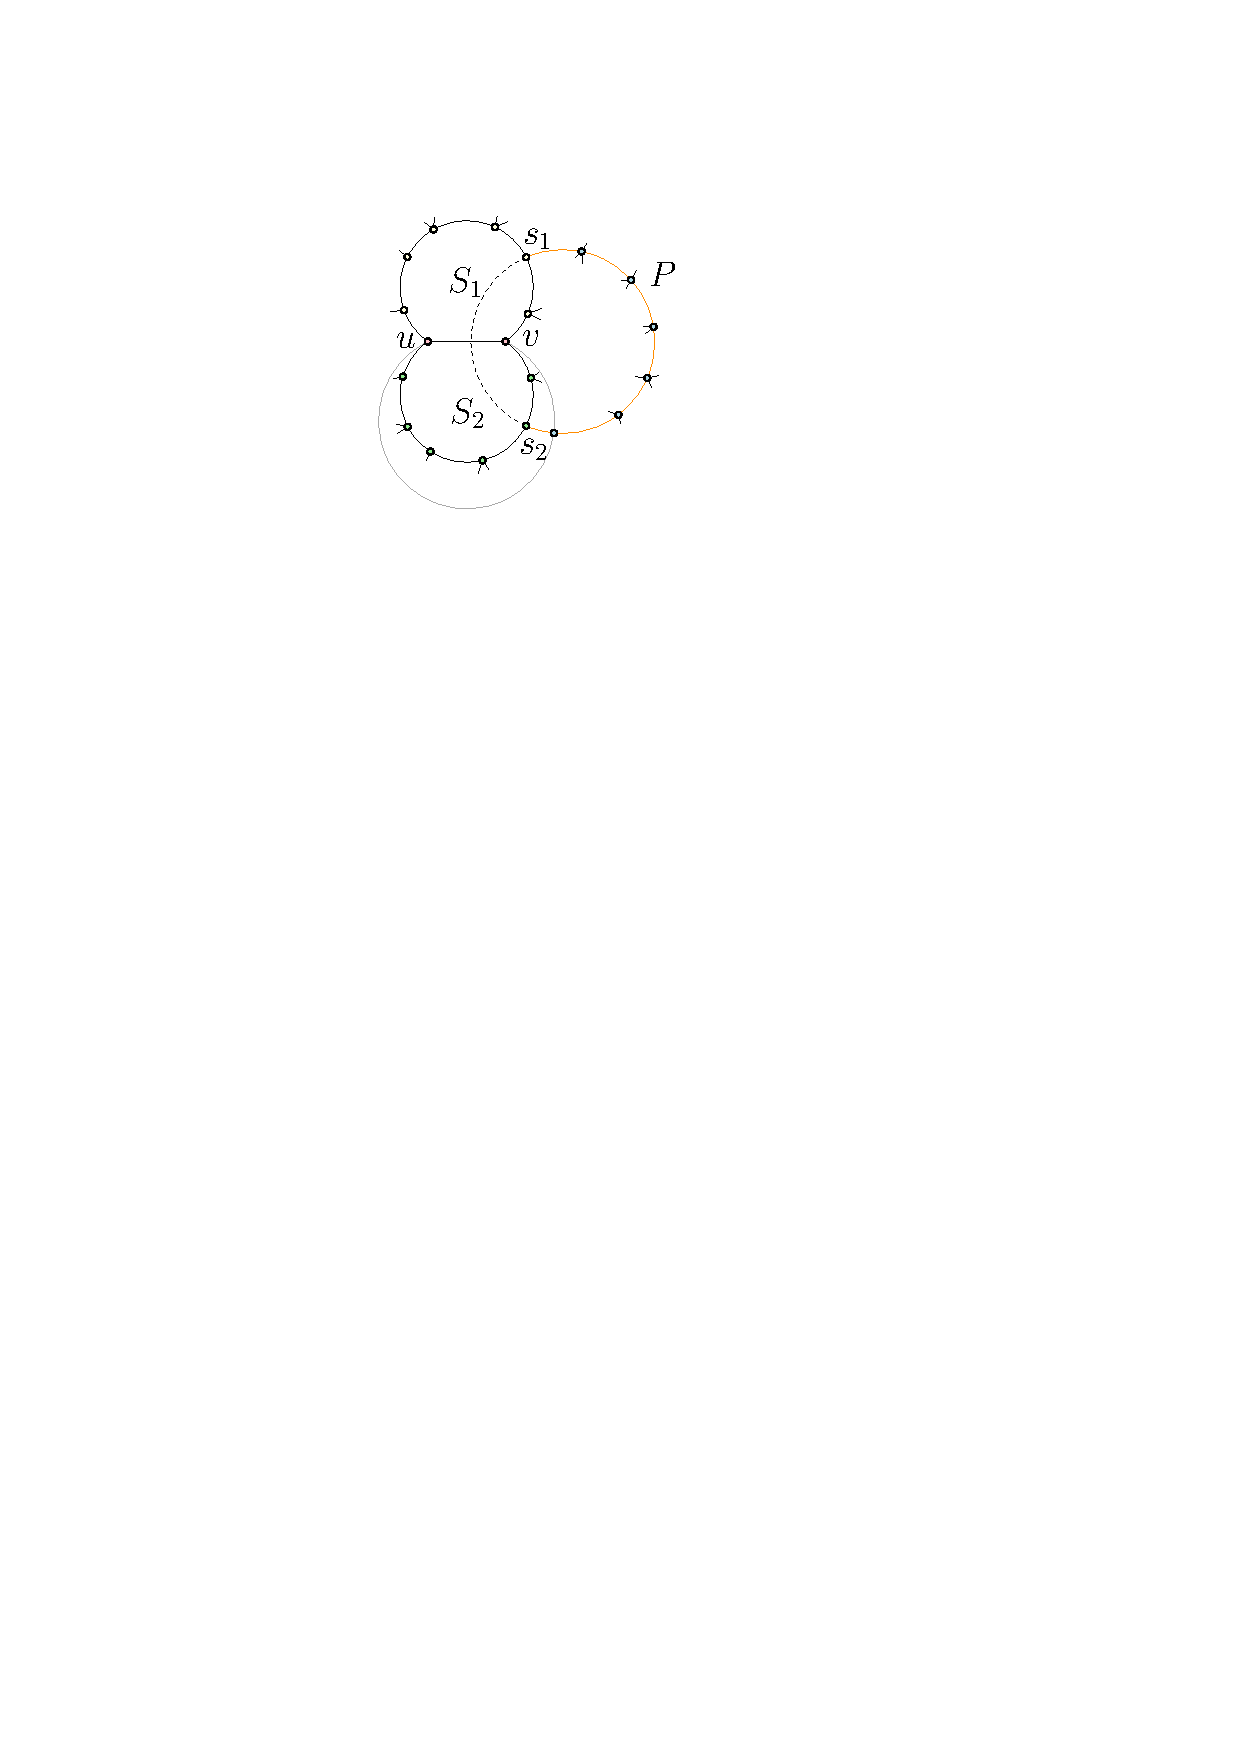
\includegraphics[width=0.21\textwidth]{figures/tutte_cycle_intersection.pdf}
\end{paracol}


%%%%%%%%%%%%%%%%%%%%%%%%%%%%%%%%%%%%%%%%%%%%%%%%%%%%%%%%%%%%%%%%%%%%%%%%コメントアウト
\begin{comment}
\paragraph{タットのばね\cref{thm:tutte}からの系}
以降のクラトフスキー定理の証明および平面性判定で用いる
タットのばね\cref{thm:tutte}の系を記述する。


\begin{corollary}
\label{coro:convex_face}
タットの平面描画の各面はいずれも凸多角形。
\end{corollary}


\begin{corollary}
\label{coro:tutte_any_face}
平面的グラフ$G$は任意の頂点を外面に持つ平面埋込みを持つ。
\end{corollary}

\cref{coro:convex_face}は
\cref{lemma:tutte_opposite}および\cref{lemma:tutte_collinear}によって保証される。
タットの平面描画は平面埋込みからの面選択に制限を課さないので
\cref{coro:tutte_any_face}は、
$1$-連結や$2$-連結なグラフであっても仮想的に辺を追加して$3$-連結にしてから
タットの平面描画を実行すると任意の包囲閉路を外面とする平面描画が得られる。
\end{comment}
%%%%%%%%%%%%%%%%%%%%%%%%%%%%%%%%%%%%%%%%%%%%%%%%%%%%%%%%%%%%%%%%%%%%%%%%コメントアウト










%%%%%%%%%%%%%%%%%%%%%%%%%%%%%%%%%%%%%%%%%%%%%%%%%%%%%%%%%%%%%%%%%%%%%%%%%%%%%%%%%%%%%%%
\subsection{クラトフスキーの定理}
\label{subsec:kuratowski}

\setcolumnwidth{0.66\textwidth, 0.33\textwidth}
\begin{paracol}{2}
ここではクラトフスキーの定理を考察する。
特にグラフが非平面的なら必ずクラトフスキー部分グラフを持つことを示す。


\begin{theorem}[クラトフスキー定理]
\label{thm:kuratowski}
グラフ$G$が平面的であることの必要十分条件は
$G$が部分グラフとして$K_5$もしくは$K_{3,3}$の細分を持たないこと。
\end{theorem}

\switchcolumn
%\vspace{1.5\intextsep}
\centering
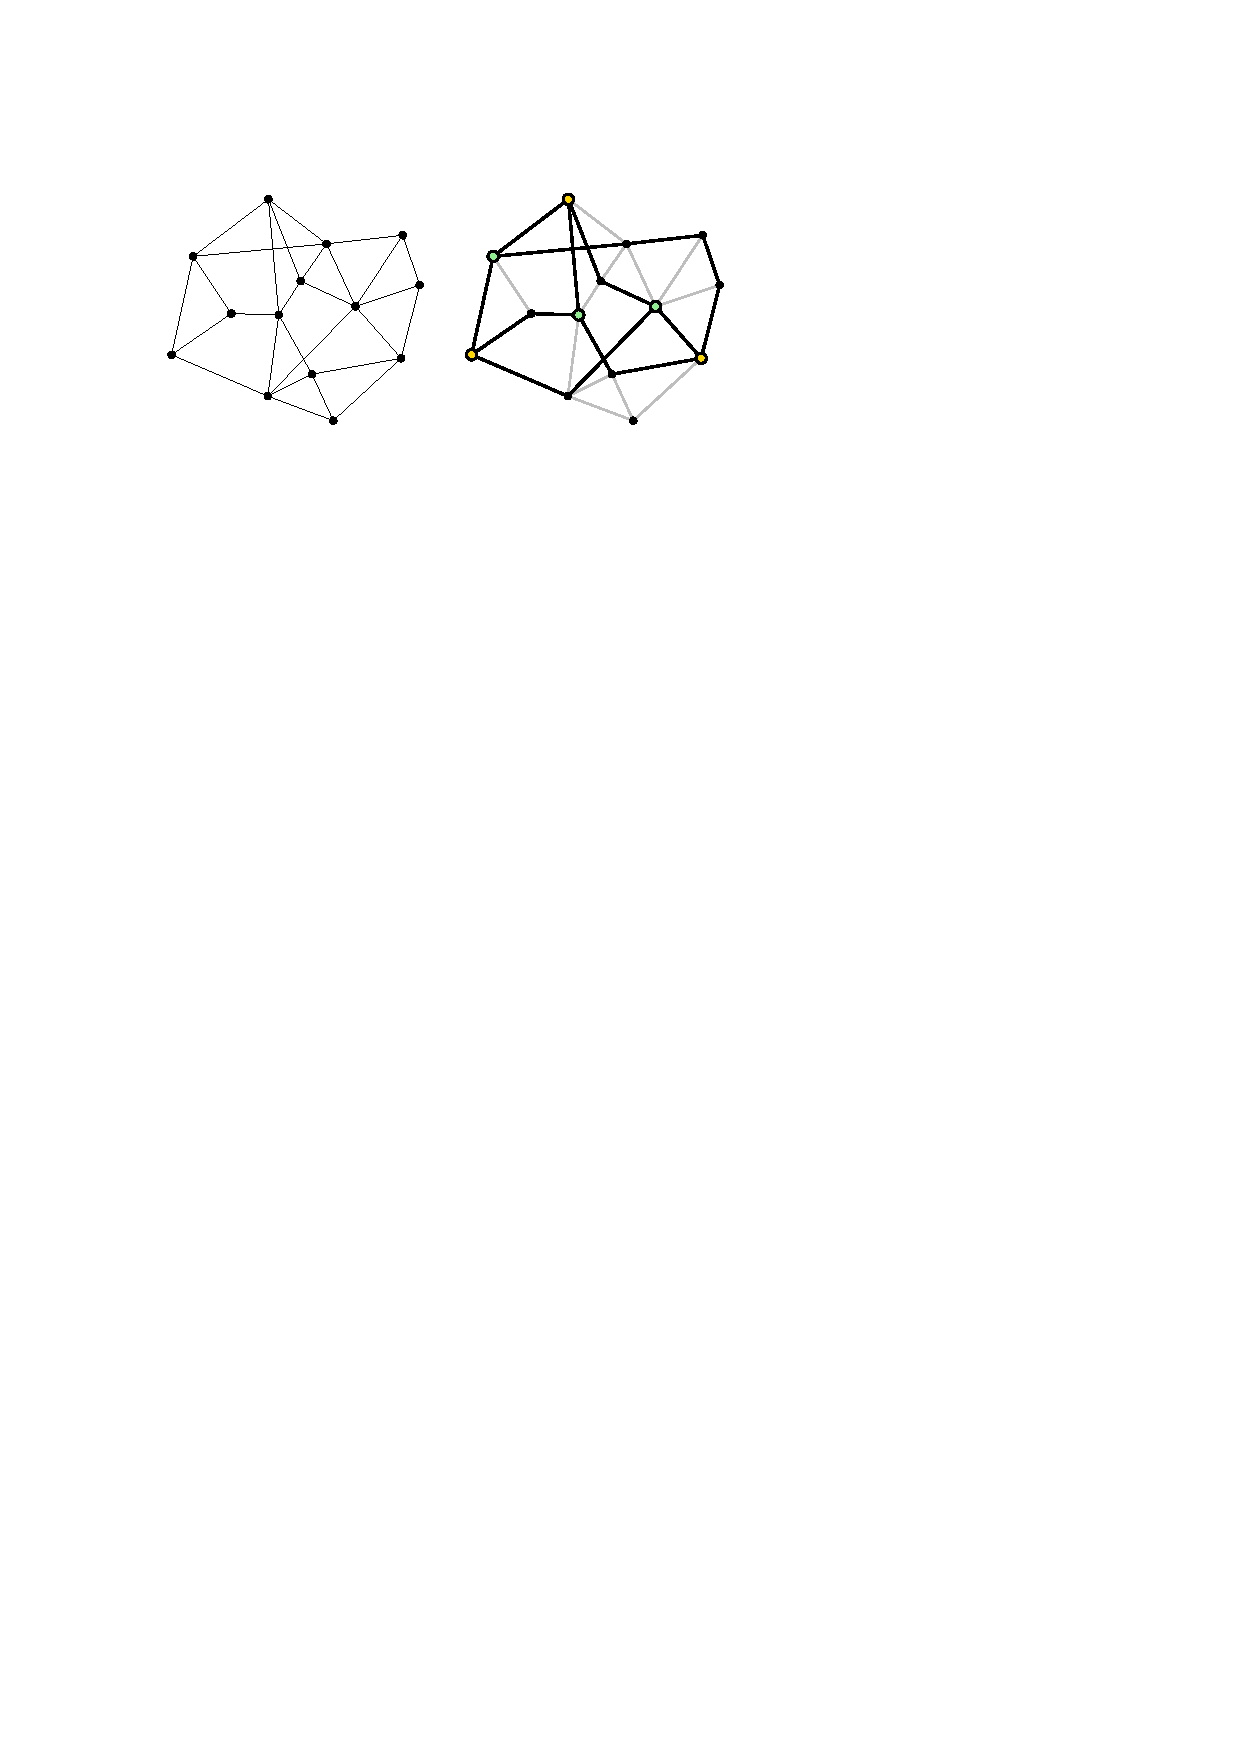
\includegraphics[width=0.3\textwidth]{figures/kuratowski_subgraph_example_01.pdf}
\end{paracol}

\paragraph{十分性の証明}
必要性はオイラーの多面体公式の\cref{coro:girth}および
辺細分による頂点数と辺数の増分差分の不変性を確認すれば帰納的に示せる。
%以下では十分性を証明する。
以下では極小な非平面的グラフを対象に議論する。
これは、どんな非平面的グラフも辺を削除していけば最終的に平面的になり、
その直前には近傍に極小性を有する部分グラフが存在することから
一般性を失わない。



\begin{lemma}[クラフトスキーの定理の十分性]
グラフ$G$が非平面的ならクラトフスキー部分グラフを持つ。
\end{lemma}

\begin{proof}
\cref{lemma:3_connectivity} は、
クラトフスキー部分グラフを持たない辺数最小の非平面的グラフが存在するなら
それは$3$-連結であることを保証する。
また、\cref{lemma:contractions_dont_make_kuratowski_subgraph}および
\cref{lemma:contractions_preserve_3_connectivity} は、
$3$-連結性を保持しつつクラトフスキー部分グラフを生成しないよう
極小非平面的グラフの辺数を可能な限り減らすことができることを保証する。
一方で\cref{lemma:tutte} は、
クラトフスキー部分グラフを持たない$3$-連結なグラフには
平面描画が存在することを保証する。
これは極小な非平面的グラフが
クラトフスキー部分グラフを持つことの証左である。
\end{proof}



%以下では極小な非平面的グラフに限定して議論する。
%頂点や辺の追加によって非平面的なグラフが平面的になったり
%クラトフスキー部分グラフが消失することはないため、
%極小なグラフに限定しても一般性を失わない。



%%%%%%%%%%%%%%%%%%%%%%%%%%%%%%%%%%%%%%%%%%%%%%%%%%%%%%%%%%%%%%%%%%%%%%%%%%%%% Lemma 2
\begin{lemma}\label{lemma:1-connected}
極小な非平面的グラフは$1$-連結。
\end{lemma}

\begin{proof}
$1$-連結でないと仮定する。
いずれの成分も非平面的なら任意の辺削除で平面的とならず極小性に反する。
同様に平面的な連結成分が存在するならその成分内の辺を削除しても平面的とはならない。
\end{proof}


%%%%%%%%%%%%%%%%%%%%%%%%%%%%%%%%%%%%%%%%%%%%%%%%%%%%%%%%%%%%%%%%%%%%%%%%%%%%% Lemma 3
\begin{lemma}\label{lemma:2-connected}
極小な非平面的グラフは$2$-連結。
\end{lemma}

\begin{proof}
$2$-連結でない、つまり切断点$v$を持つ極小な非平面的グラフ $G=(V, E)$ が存在すると仮定する。
$C \subseteq V$ を $G \setminus v$ の任意の連結成分の頂点集合とする。
このとき誘導部分グラフ$G[C \cup \{v\}]$および$G \setminus C$は
互いに辺素なので
\cref{lemma:1-connected} の証明と同様の議論により極小性に反する。
\end{proof}



%%%%%%%%%%%%%%%%%%%%%%%%%%%%%%%%%%%%%%%%%%%%%%%%%%%%%%%%%%%%%%%%%%%%%%%%%%%%%%%%%%% Lemma 4
\begin{lemma}\label{lemma:edge_disconnected}
$G=(V, E)$ を非平面的グラフとする。
$x, y \in V$ を $G' = G \setminus \{x, y\}$ が非連結となる頂点対とする。
このとき、次を満たす $G'$ の連結成分$C \subseteq V$ が存在する。
$C \cup \{x, y\}$ および辺 $(x, y)$ が誘導する部分グラフが非平面的。
\end{lemma}

\vspace*{-\intextsep}
\setcolumnwidth{0.8\textwidth, 0.2\textwidth}
\begin{paracol}{2}
\begin{proof}
$C_1, \ldots, C_k$ を $G'$ の連結成分とする。
$G'_i$ を $C_i \cup \{x, y\}$ に辺$(x,y)$を加えて誘導される部分グラフとする。
各 $G'_1, \ldots, G'_k$ はいずれも平面的と仮定する。
このとき$H_1$ を $G'_1$ の平面描画とすると、
$2 \leq i \leq k$ に関して $H_{i-1}$ の $(x, y)$ を含むいずれかの面の内部に
$G'_i$ を描画して得られる平面描画 $H_i$ が存在する。
帰納的に$H_k - (x, y)= G$ は平面的であるがこれは主張の前提に反する。
\end{proof}

\switchcolumn
%\begin{figure}[ht]
\centering
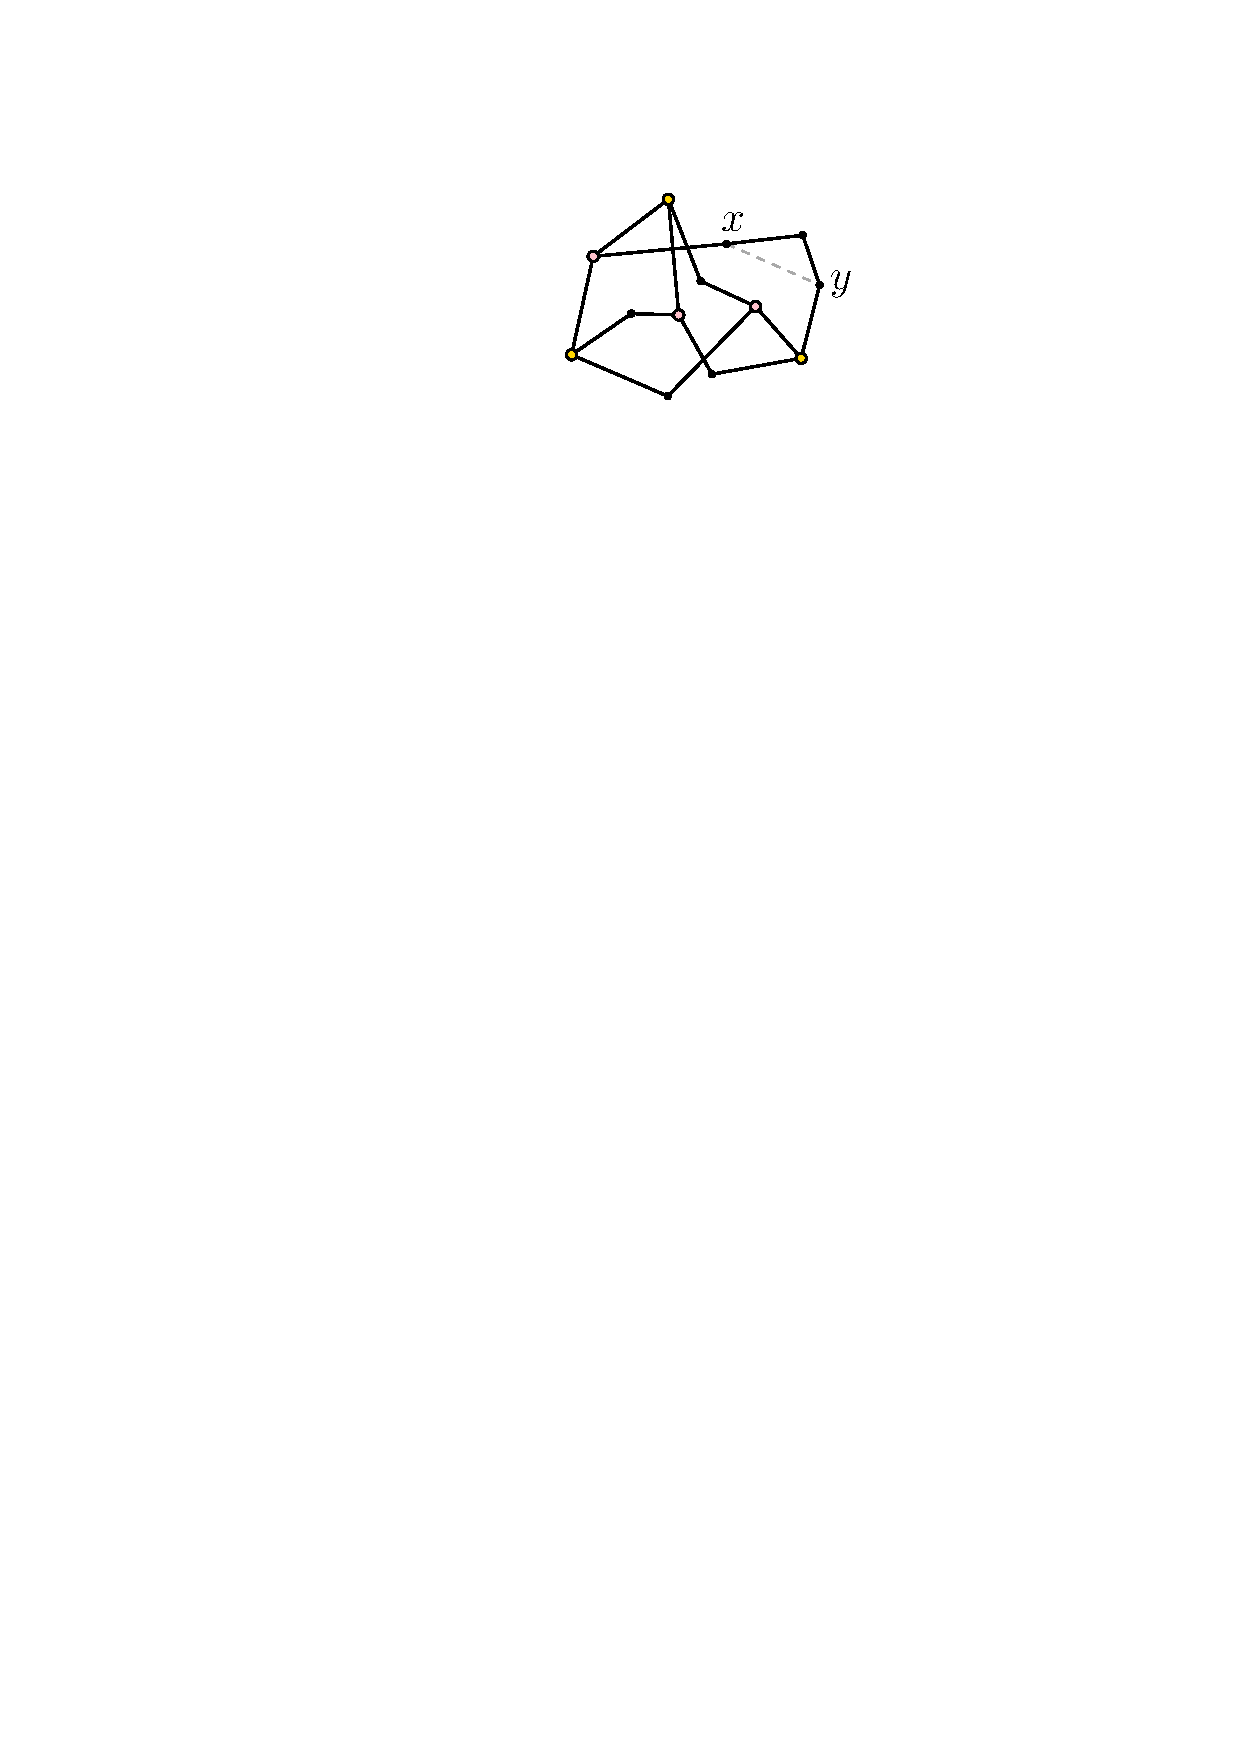
\includegraphics[width=0.18\textwidth]{figures/kuratowski_subgraph_example_02.pdf}
%\end{figure}
\end{paracol}


%%%%%%%%%%%%%%%%%%%%%%%%%%%%%%%%%%%%%%%%%%%%%%%%%%%%%%%%%%%%%%%%%%%%%%%%%%%%%%%%% Lemma 5
\begin{lemma}\label{lemma:3_connectivity}
$G = (V, E)$ をクラトフスキー部分グラフを持たない
すべての非平面的グラフの中で辺数最小のグラフとするなら、
$G$は$3$-連結。
\end{lemma}

\begin{proof}
$G$は極小なので\cref{lemma:2-connected}~より$2$-連結。
$G$ を非連結にする二頂点 $x, y \in V$ が存在すると仮定すると、
$G\setminus \{x, y\}$ は連結成分 $C_1, \ldots, C_k$ を持つ。
\cref{lemma:edge_disconnected} より
$C_i \cup \{x, y\}$ に辺 $(x,y)$を加えて誘導される部分グラフ $H$ が
非平面的となる $C_i$ が存在する。
$G$ の辺数最小性より $H$ はクラトフスキー部分グラフ $K$ を持つが、
$(x, y) \notin E$なので $K$ は $G$ の部分グラフではない。
$G$は$2$-連結なので、メンガーの\cref{thm:menger}より、
別の連結成分 $C'$ の頂点のみで構成される $x$ と $y$ をつなぐパス $P$ が存在する。
$K$ と $P$ をつなぎ合わせると$G$内にクラフトスキー部分グラフを得る。
\end{proof}


%%%%%%%%%%%%%%%%%%%%%%%%%%%%%%%%%%%%%%%%%%%%%%%%%%%%%%%%%%%%%%%%%%%  Menger

\begin{comment}
上記の証明では暗にメンガーの定理を利用している。

\begin{theorem}[メンガーの定理]
グラフが$k$-連結である必要十分条件は、任意の二頂点間に$k$個の点素パスが存在すること。
\end{theorem}
\end{comment}


%%%%%%%%%%%%%%%%%%%%%%%%%%%%%%%%%%%%%%%%%%%%%%%%%%%%%%%%%%%%%%%%%%%%%%%%%% Lemma 6
\begin{lemma}\label{lemma:contractions_dont_make_kuratowski_subgraph}
$G = (V, E)$ をクラトフスキー部分グラフを持たないグラフとする。
任意の辺 $e \in E$ を縮約してもクラフトスキー部分グラフにはならない。
\end{lemma}

\vspace*{-\intextsep}
\setcolumnwidth{0.7\textwidth, 0.3\textwidth}
\begin{paracol}{2}
\begin{proof}
$G / e$と$v_e$をそれぞれ$e=(x, y) \in E$ を縮約して得られるグラフと頂点とする。
$G/e$ がクラトフスキー部分グラフ$H$を持つと仮定する。
%頂点 $v_e$ を辺$e$を縮約して得られる頂点とし次数を$d(v_e)$とする。
$v_e$ が $H$ の頂点でないなら $H$は$G$の部分グラフとなり矛盾。
$H$の最小次数は$2$、最大次数は$4$なので $2 \leq \deg(v_e) \leq 4$。
$\deg(v_e) = 2$なら$x$と$y$の縮約前の次数の組合せは、
$\deg(x) = \deg(y) = 2$もしくは一方が$1$か$3$の場合である。
いずれも$G$は$H$の細分か同型な部分グラフを持つこととなり矛盾。
$\deg(v_e)\geq 3$で$x, y$のいずれかの次数が$\deg({v_e})$以上の場合、
$H$の細分は$G$の部分グラフとなるので矛盾(右図上段)。
$H$が$K_5$の細分であり、$\deg(x) = \deg(y) = 3$の場合、
$G$は$K_{3,3}$の細分を持つので矛盾(右図下段)。
\end{proof}


\switchcolumn
%\begin{figure}[h]
\vspace{0.5\intextsep}
\centering
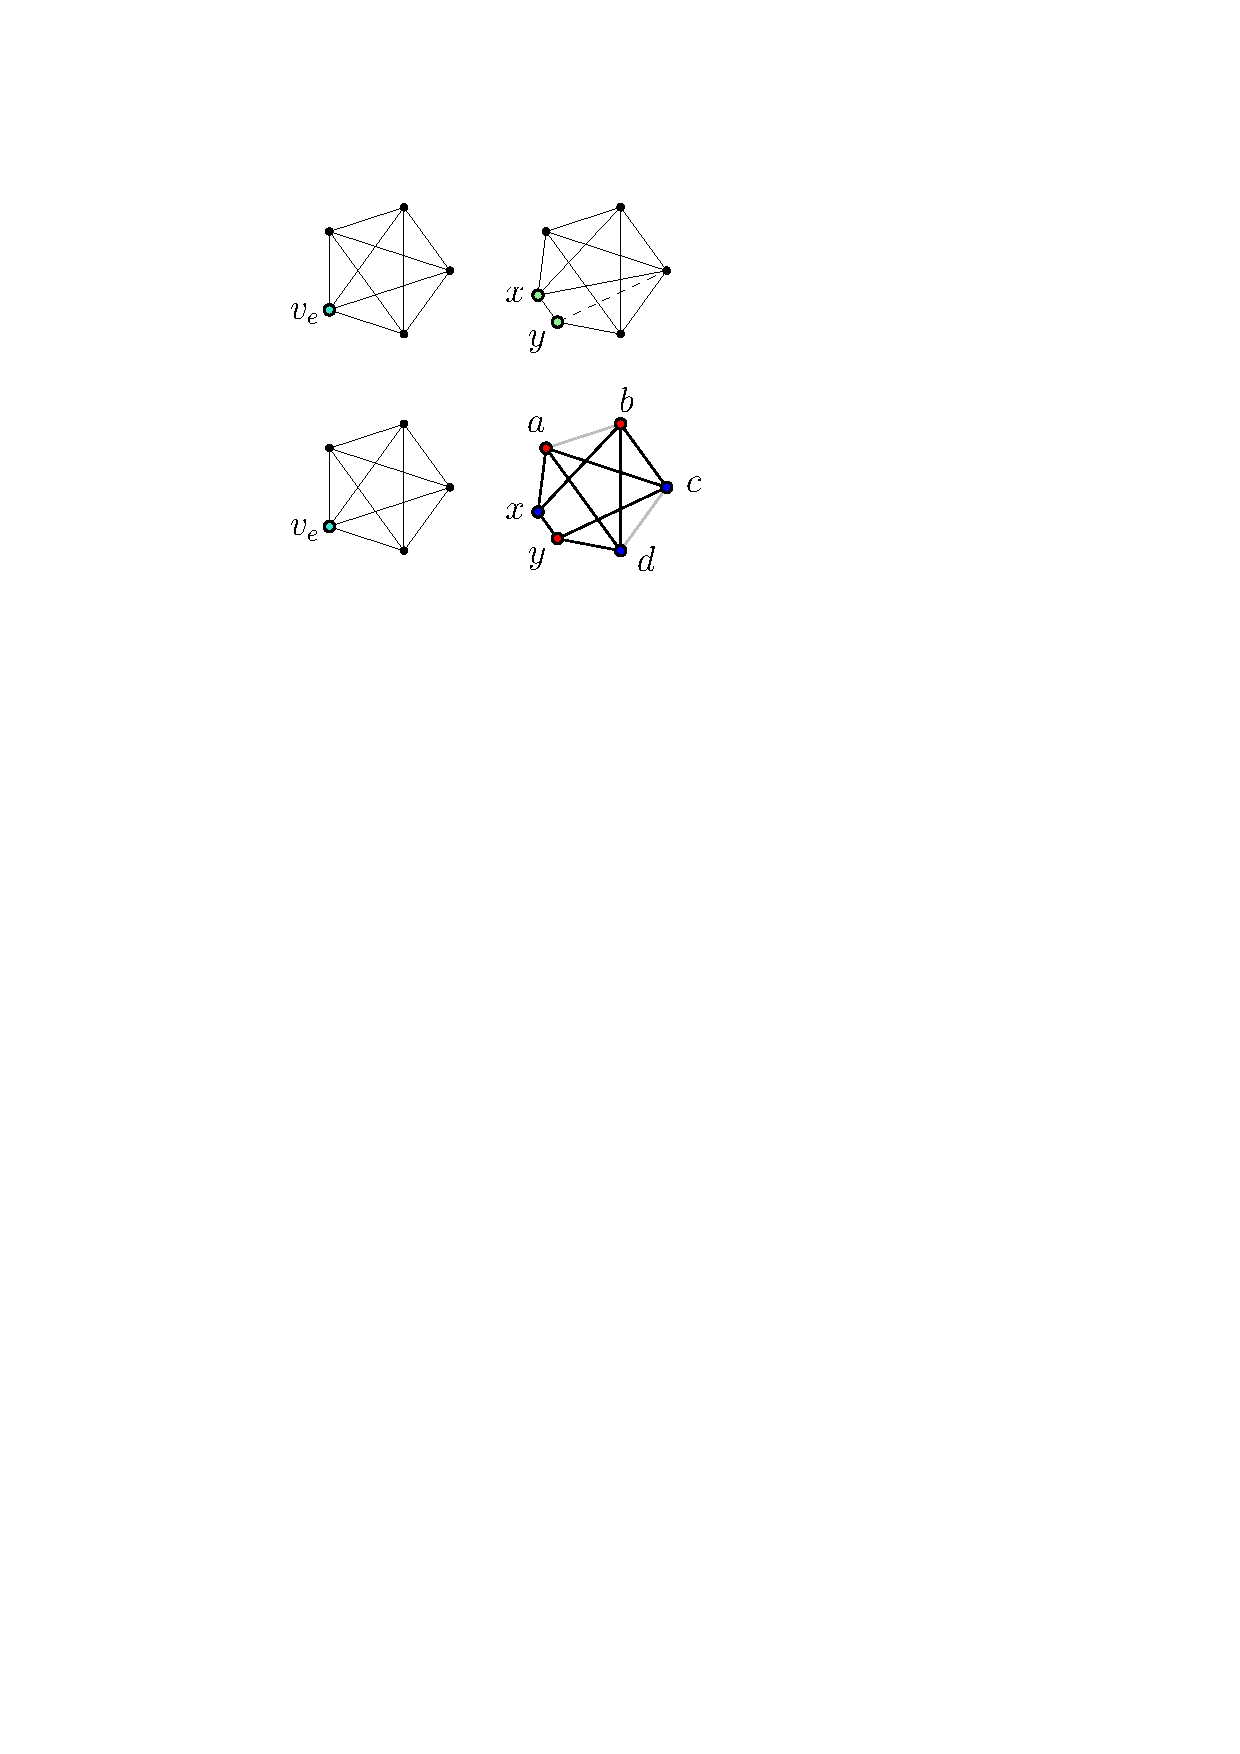
\includegraphics[width=0.25\textwidth]{figures/contraction_01.pdf}
%\end{figure}
\end{paracol}



%%%%%%%%%%%%%%%%%%%%%%%%%%%%%%%%%%%%%%%%%%%%%%%%%%%%%%%%%%%%%%%%%%%%%%%%%%%%%%%%%% Lemma 7
\begin{lemma}\label{lemma:contractions_preserve_3_connectivity}
$G = (V, E)$ を$|V| \geq 5$の$3$-連結なグラフとする。
$G$ は縮約しても$3$-連結性を損なわない辺を持つ。
\end{lemma}



\vspace*{-\intextsep}
\setcolumnwidth{0.75\textwidth, 0.25\textwidth}
\begin{paracol}{2}
\begin{proof}
どの辺$e\in E$を縮約対象に選んでも$3$-連結性を損なう$G$が存在すると仮定する。
このとき、どの辺$e=(x, y)$にも
$G \setminus \{x, y, \delta(e)\}$で非連結になる頂点$\delta(e)\in V$が存在する。
$C_e$を$G \setminus \{x, y, \delta(e)\}$内で頂点数最大の連結成分の頂点集合とする。
%
%$v_e$を$e$の縮約で生成される頂点とすると$G / e \setminus \{v_e, \delta(e)\}$が
%非連結となる頂点$\delta(e) \in V$が存在する。
%$G'=G/e$とし$v_e$を$e$を縮約して得られる頂点とする。
%任意の$e=(x, y)\in E$に関して$G'$が$3$-連結ではないと仮定すると
%$G'\setminus \{v_e, z_e\}$が非連結となる頂点$z_e\in V$が存在し、
%$\{x, y, z_e\}$の削除で$G$は非連結となる。
%任意の辺$e=(x, y)$に対して
%
%任意の辺$e=(x, y)$が与えられたとき
%$C_e$ を$G \setminus \{x, y, z_e\}$内の最も大きな連結成分とする。
%$C_e$ は背理法の仮定の下で well-defined。
%以下、
$e^* = \argmax_{e \in E} (|C_e|)$とする。
$C'$を$G\setminus \{x, y, \delta(e^*)\}$の$C_{e^*}$以外の連結成分とする。
$G$は$3$-連結なので$\delta(e^*)$と$u \in C'$を接続する辺$f$が存在する。
$f$についても同様に$G$を非連結にする頂点$\delta(f)$が存在する。
$G[C_{e^*} \cup \{x, y\}]$は$2$-連結で$\delta(f)$を削除しても連結性を失わないので
$G\setminus \{\delta({e^*}), u, \delta(f)\}$は少なくとも頂点数
$|C_{e^*} \cup \{x, y\}|-1$の連結成分を持つが、これは$C_{e^*}$の最大性に矛盾する。
\end{proof}

\switchcolumn
\vspace{1\intextsep}
%\begin{figure}[ht]
\centering
%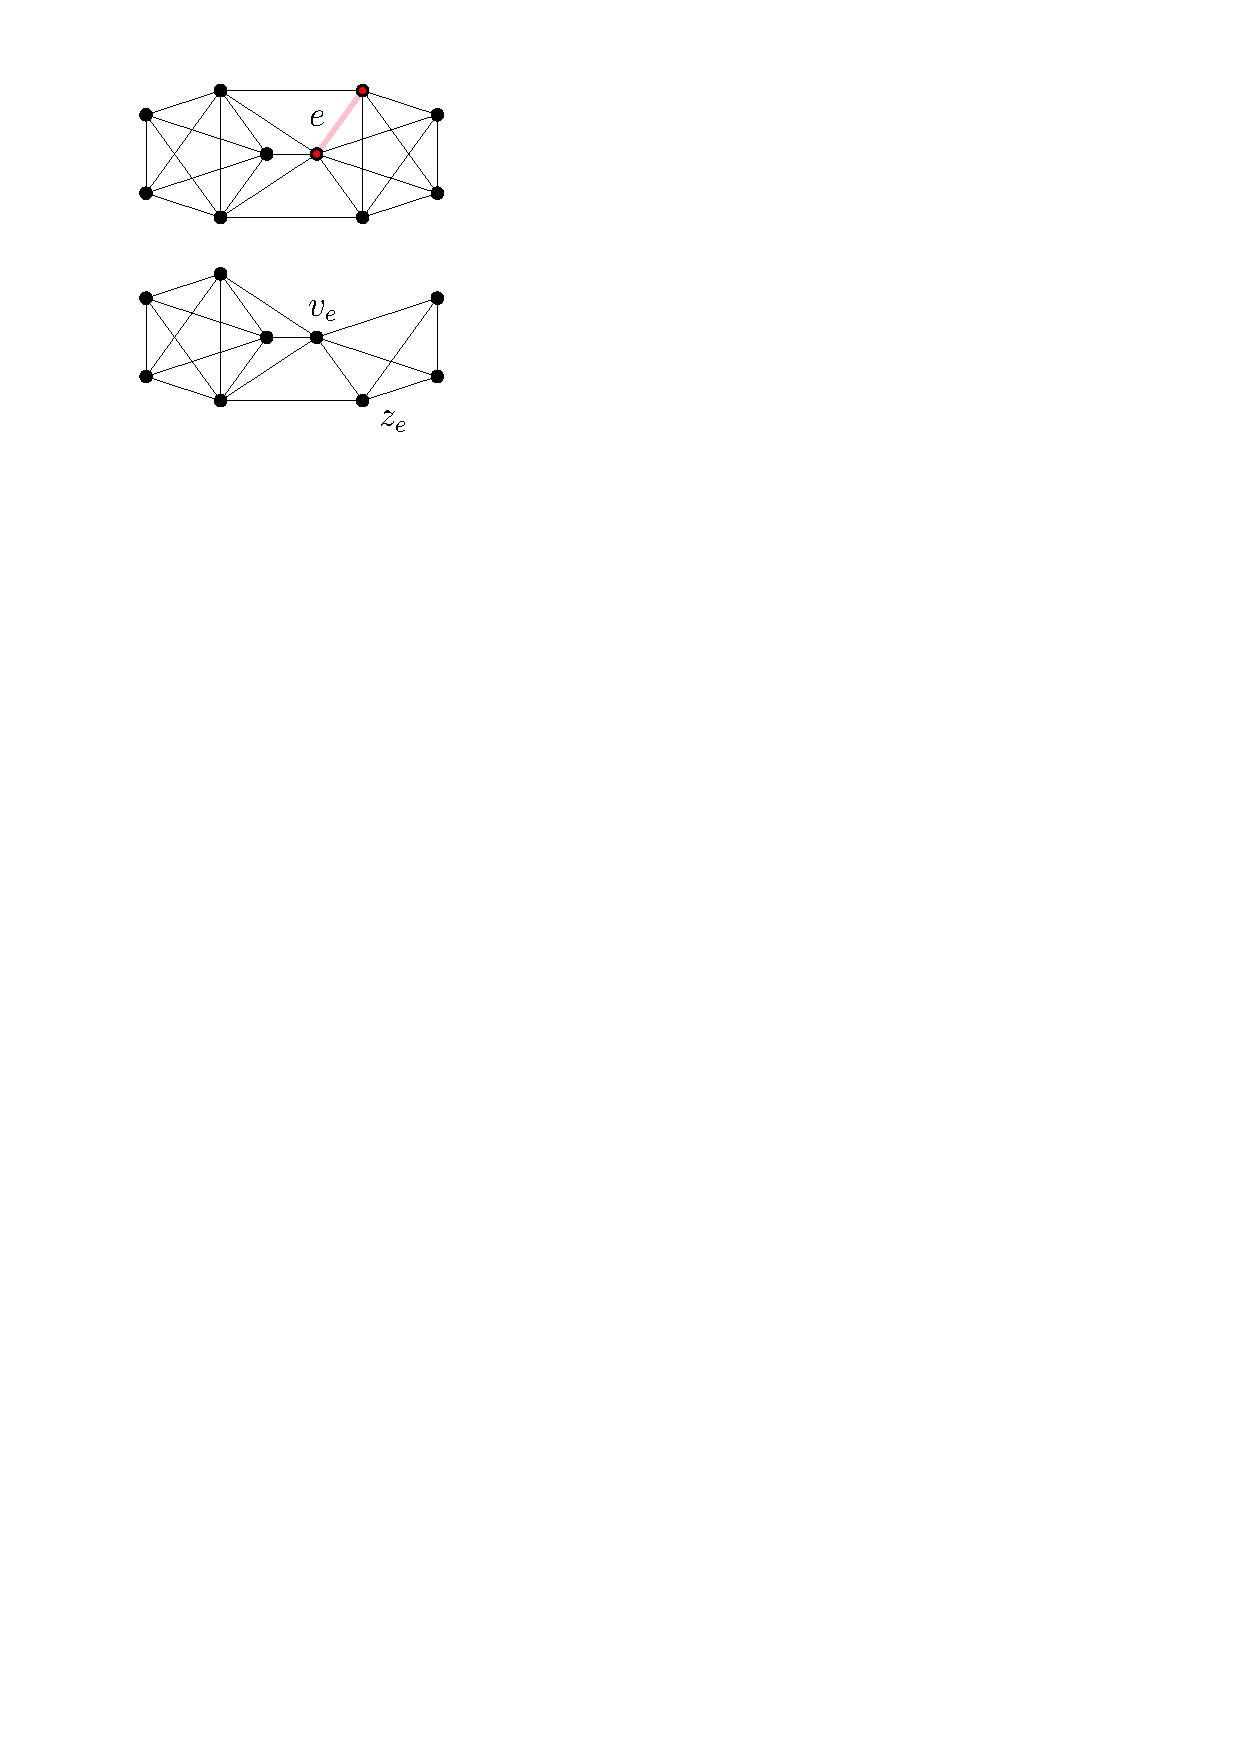
\includegraphics[width=0.14\textwidth]{figures/contractions_and_3_connectivity_01.pdf}
%\end{figure}


%\begin{figure}[ht]
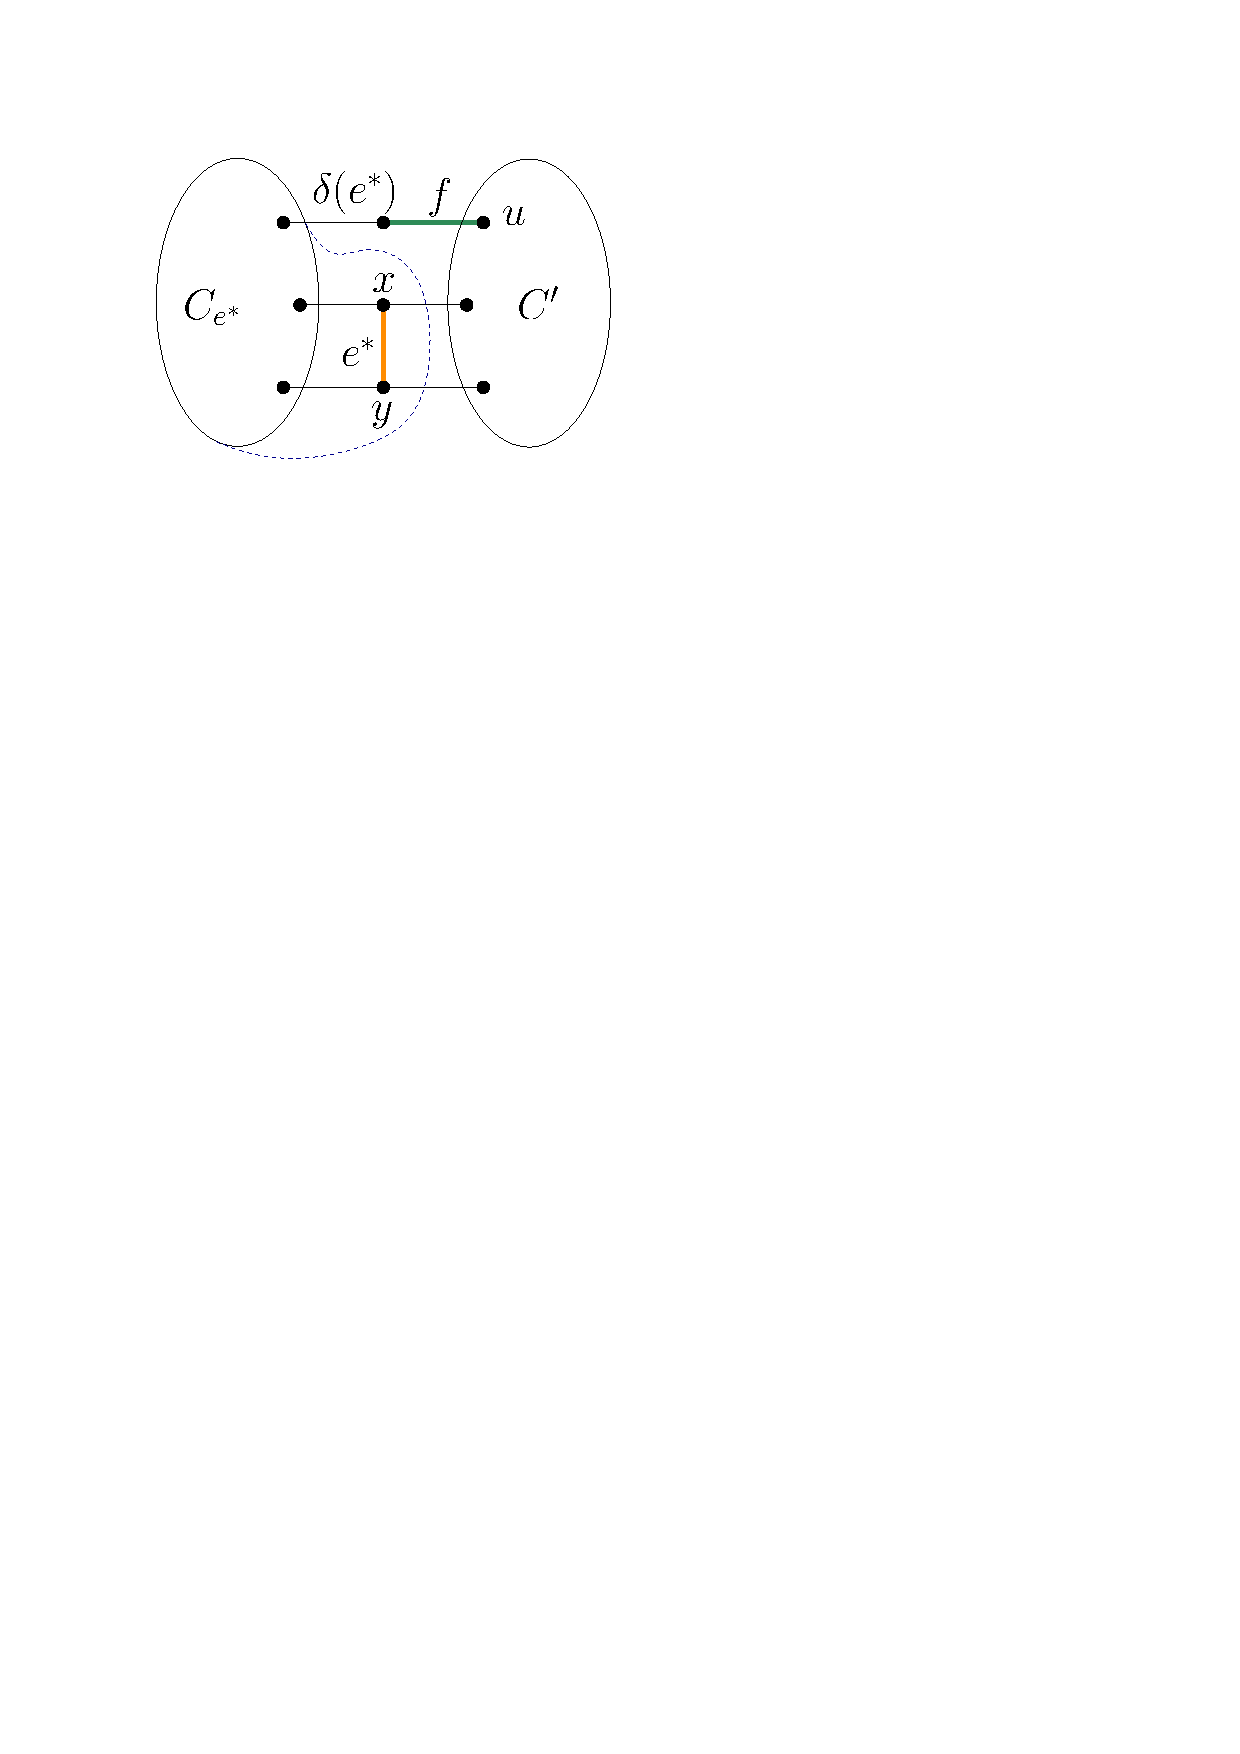
\includegraphics[width=0.24\textwidth]{figures/contractions_and_3_connectivity_03.pdf}
%\end{figure}
\end{paracol}



%%%%%%%%%%%%%%%%%%%%%%%%%%%%%%%%%%%%%%%%%%%%%%%%%%%%%%%%%%%%%%%%%%%%%%%%%% Tutte
\begin{lemma}\label{lemma:tutte}
$G = (V, E)$ が$3$-連結でクラトフスキー部分グラフを持たないなら、
$G$は平面埋込みを持つ。
\end{lemma}



\vspace*{-\intextsep}
\setcolumnwidth{0.82\textwidth, 0.18\textwidth}
\begin{paracol}{2}

\begin{proof}
頂点の個数に関する帰納法を用いる。
最小の$3$-連結グラフは$K_4$であり、
これは三頂点を適当に配置した後に残りの頂点を重心に配置することで平面埋め込みを得る。

$G = (V, E)$ に平面埋込みが存在することを示すために、
ある辺$e\in E$の縮約$G / e$が平面埋込みを持つと仮定する。
$v_e$ を$e=(x,y)$を縮約することで得られる$G / e$の頂点とする。
$G/e$は\cref{lemma:contractions_preserve_3_connectivity}より$3$-連結なので、
$v_e$ を除去すると多角形としての面$f$が出現する。

系列$(x_1, \ldots, x_k)$ を$x$に隣接する頂点で
$f$に沿った整列とする。
$y$ のすべての隣接頂点$y_1, \ldots, y_\ell$が$x_i$と$x_{i+1}$の間に配置されるなら、
$x$を$v_e$の位置に$y$を$x, y_1, \ldots, y_\ell$ の重心に配置することで
$G$ の平面埋込みを得る。
それ以外の二通りの場合はいずれも主張の前提に反する。
一つは、$x, y$が少なくとも3つの共通する隣接頂点を持つ場合で、
これは$G$が$K_5$の細分を持つ。
他方は、$x_i \neq y_1$および$x_{i+1} \neq y_\ell$の下で
$f$の境界上に
$x_i, y_1, \ldots, x_{i+1}, \cdots, y_\ell$の順で並んでいる場合で、
これは$G$が$K_{3,3}$の細分を持つ。
\end{proof}

%凸配置に関する言及はタットのばね定理に従う。

\switchcolumn
\vspace{0.5\intextsep}
\centering
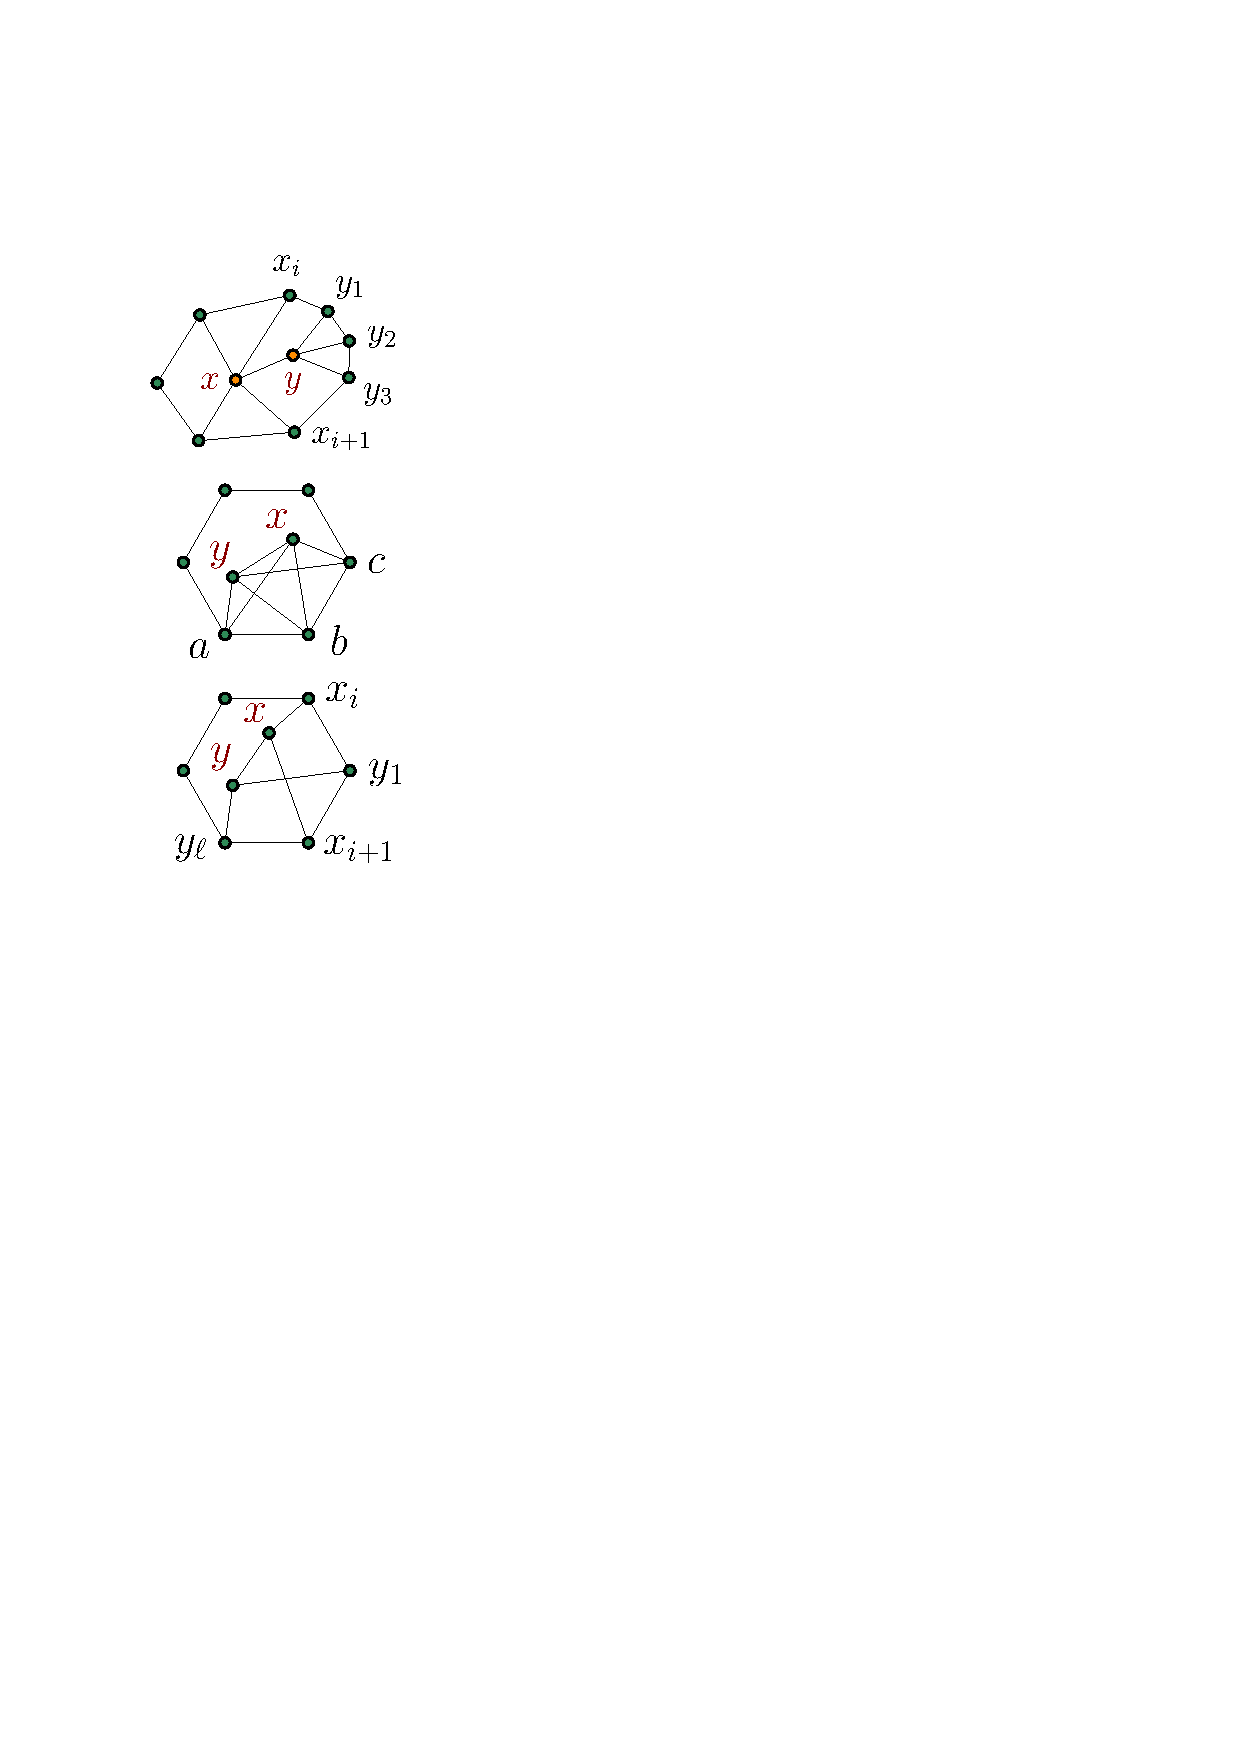
\includegraphics[width=0.12\textwidth]{figures/convex_embedding.pdf}
\end{paracol}

\begin{comment}
%\vspace*{-\intextsep}
\setcolumnwidth{0.85\textwidth, 0.15\textwidth}
\begin{paracol}{2}
\begin{theorem}[タットのばね定理]
単純で$3$-連結な平面的グラフは次の特徴を有する平面描画を持つ。各辺は直線分。
外面は凸多角形。内部の頂点は隣接頂点の重心。
\end{theorem}

\switchcolumn
\vspace*{-0.5\intextsep}
\begin{figure}[ht]
\centering
\includegraphics[width=0.12\textwidth]{figures/tutte_embedding_error.png}

{\small フルフトグラフの凸埋め込み}
\end{figure}

\end{paracol}

\end{comment}


\newpage


\section{深さ優先探索}

この節では平面性判定を解決する線形時間アルゴリズムを設計するために、
基本的な枠組みである深さ優先探索について考察する。
また、深さ優先探索の応用として
グラフの$2$-辺連結性を線形時間で判定するアルゴリズムを与える。






%%%%%%%%%%%%%%%%%%%%%%%%%%%%%%%%%%%%%%%%%%%%%%%%%%%%%%%%%%%%%%%%%%%%% 深さ優先探索
\subsection{深さ優先探索の基本原理}
%平面性判定に入る前に、軽く$2$-辺連結性判定に触れておく。
%グラフが$2$-辺連結であるかどうかは橋の有無で判定できる。
%橋はそれを除去すると連結成分の個数を1つ増やす辺である。
%橋検出は深さ優先探索で$O(n+m)$時間で解決することができる。
%$n,~m$はそれぞれ頂点と辺の個数。
%\vspace*{-0.7\intextsep}
\setcolumnwidth{0.75\textwidth, 0.25\textwidth}
\begin{paracol}{2}

深さ優先探索は、任意の頂点から探索を開始し、
まだ訪問していない頂点$v$を発見したら直ちに$v$に遷移し、
新たに$v$の隣接頂点の中から未訪問の頂点を見つけようとする探索方法である。
ただし、すべての隣接頂点が訪問済みならまだ調べ終わっていない頂点まで
戻って探索を再開する。
探索を開始する頂点を根と呼ぶ。

\paragraph{深さ優先探索木}
対象のグラフの各辺は頂点遷移に従い向き付けされ、
根と今調べている頂点の間には常に有向パスが存在することが保証できる。
このとき頂点発見に貢献した辺の集まりが誘導する部分グラフは有向木となる。
この有向木を深さ優先探索木と呼ぶ。
深さ優先探索木を構成する辺を木辺、それ以外の念のため調べてみたが既に発見済みの頂点だった
辺を補木辺という。
%補木辺という呼称は、対象グラフ$G=(V, E)$が連結である場合DFS木は全域木であり、
%木辺と補木辺の集合は$E$の集合分割となる。
%このとき補木辺の集合は、木辺集合の補集合として参照できることから採っている。


\switchcolumn
\vspace{-2.\intextsep}
\begin{figure}[ht]
\centering
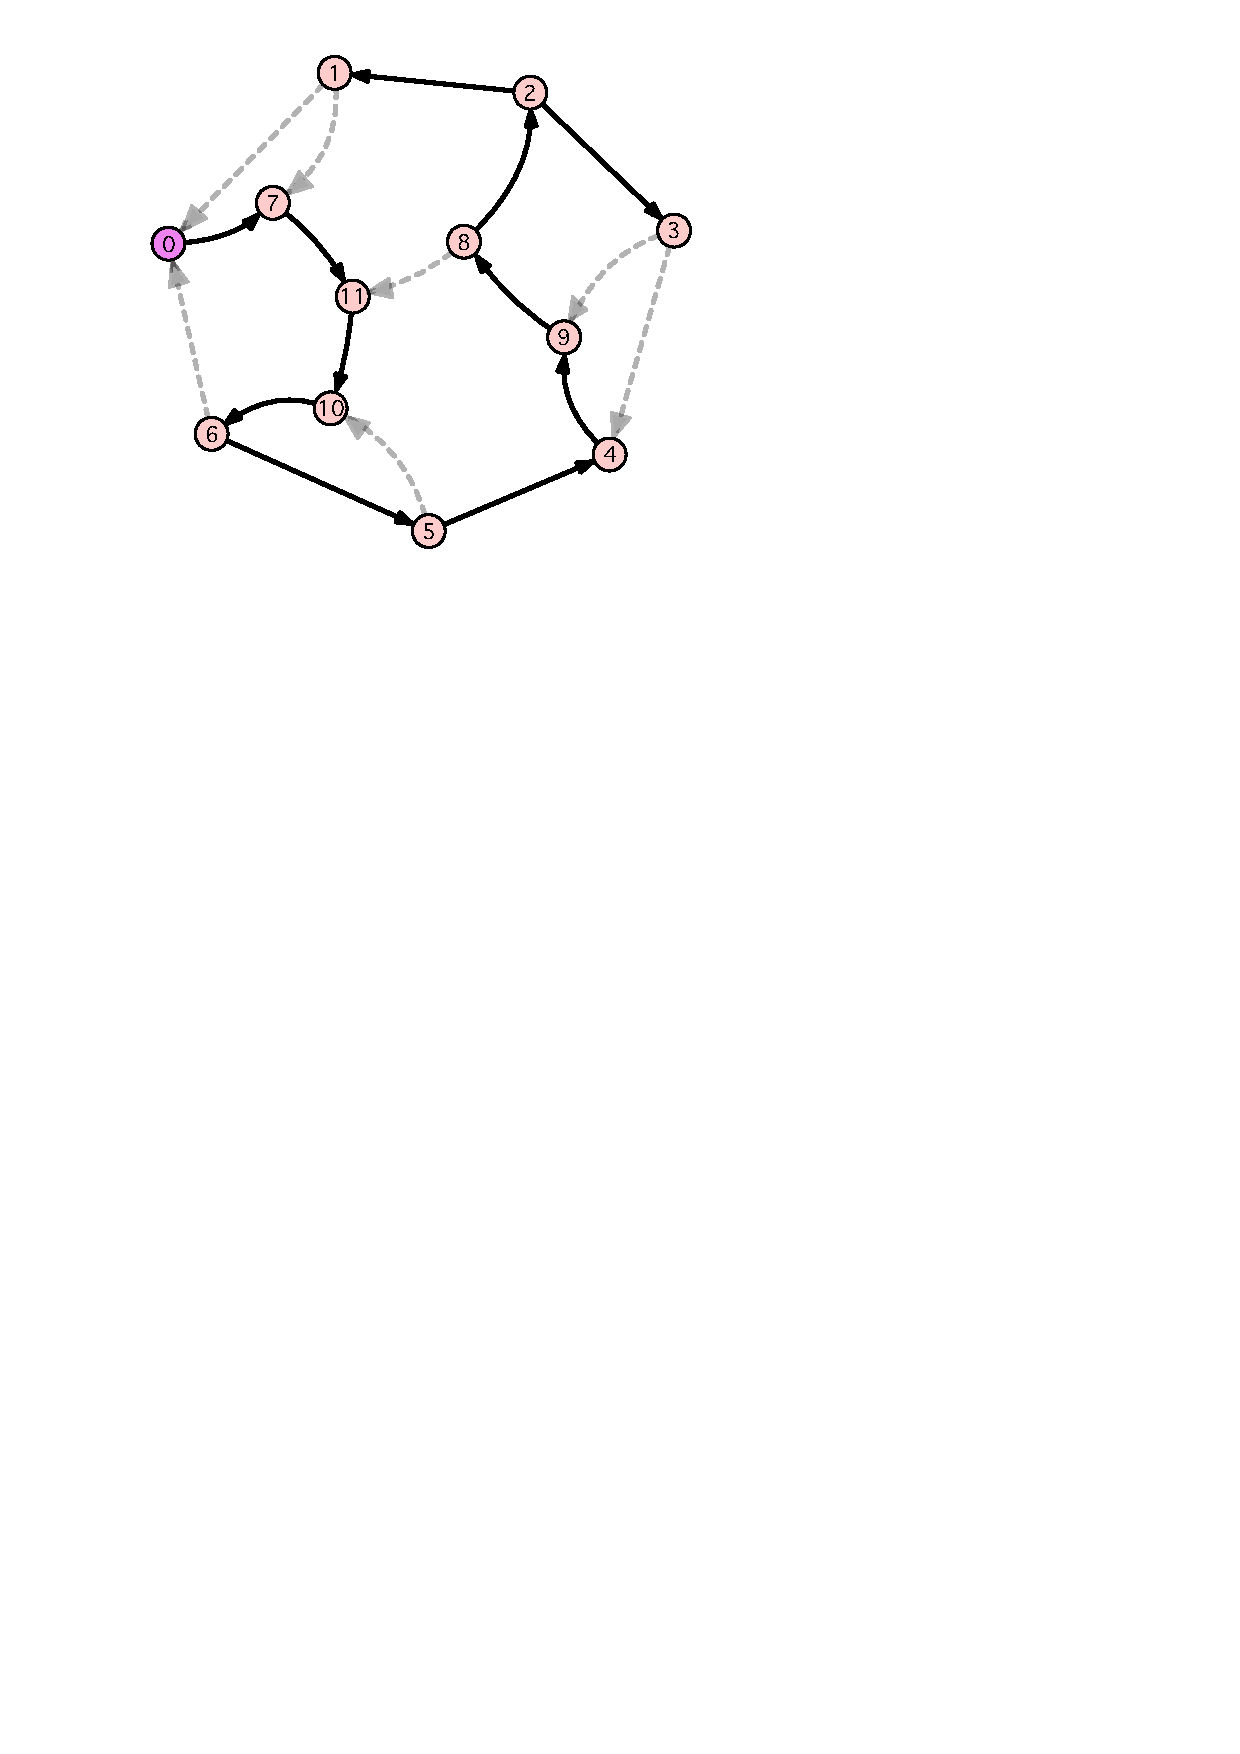
\includegraphics[width=0.24\textwidth]{figures/dfs_frucht2.pdf}
{\small フルフトグラフの\\深さ優先探索木の例}
%\label{fig:frucht_dfs_tree}
\end{figure}
\end{paracol}



\paragraph{深さ優先探索の基本コード}
下記の python コードは深さ優先探索の基本的な例である。
入力としてグラフ{\tt G}と根{\tt root}が与えられたとき、
{\tt G}において{\tt root}から到達可能な連結成分内の木辺と補木辺を表示する。
%木辺は未訪問の頂点の発見に貢献した辺で、それ以外は補木辺という。
%木辺という名称は、
%深さ優先探索の結果得られる木辺集合が誘導する部分グラフが
%対象グラフの全域木になっていることに由来する。
%補木辺は木辺集合の補集合に属すことから採っている。

\begin{lstlisting}[language=Python, caption=深さ優先探索の基本形,label=lst:dfs]
def dfs(G, root):
    stack, dfs_height = [(root, x) for x in G.neighbors(root)], {x: -1 for x in G}
    dfs_height[root] = 0
    while stack:
        parent, child = stack.pop()
        if dfs_height[child] < 0:
            stack += [(child, x) for x in G.neighbors(child) if x is not parent]
            dfs_height[child] = dfs_height[parent] + 1
            print((parent, child), ' is a tree edge')
        else:
            if dfs_height[parent] > dfs_height[child]:
                print((parent, child), ' is a back edge')
\end{lstlisting}%
%
\paragraph{コードの簡単な解説}
このコードでは、訪問すべき頂点対を管理する
データ構造としてスタック{\tt stack}を用いている(第2行)。
頂点対を対象とする理由は、
木辺と補木辺の組合せ構造がグラフの構造的性質を分析する一助となるからである。


また、訪問していない頂点を識別するために根からの距離を保持する連想配列
{\tt dfs\_height}を用いている(第2行)。
初期値を$-1$として、第6行目のように${\tt dfs\_height[child]} < 0$で
具体的に訪問していない頂点かどうかを判定する。
この判定が真となるなら{\tt (parent, child)}の頂点対は木辺であり、
偽なら終点{\tt child}の方が始点{\tt parent}より根に近いという条件付きで
補木辺と判定する(第11行)。

第6-9行は木辺に対する処理である。
つまり新たに未訪問の頂点$v$を発見したことを意味する。
このとき$v$と隣接する頂点のペアを作ってスタックに載せていく。
第5行目のスタックから頂点対{\tt (parent, child)}を取り出す処理は、
グラフ上では頂点{\tt parent}に遷移したことを意味する。

\paragraph{計算時間}
\lstrefname\ref{lst:dfs}の計算量は連結グラフを対象とするなら$O(m)$となる。
$m$は辺の個数。
これは、どの辺もスタックに追加される回数は1回、
取り除かれる回数も1回であることから測られる。
それ以外の隣接頂点リストの取得{\tt G.neighbors}、
スタックへの追加{\tt append}や削除{\tt pop}、
および連想配列の参照と更新{\tt dfs\_height[child]}は
単位時間で処理できるものとする。
%計算量に$n$が付記されているのは、$n < m$ のような非連結なグラフで、
%第7行目のスタック更新の際、結果として新たに追加する辺がない場合を考慮している。




%ここで、深さ優先探索木における半順序$\preceq$を定義する。



\paragraph{バックトラッキング}
深さ優先探索におけるバックトラックは、
子孫の部分木内のすべての頂点を訪問し終えた段階で行う処理工程をいう。
\lstrefname\ref{lst:dfs}はバックトラックを省略しているが、
下記の python コードのようにジェネレータ({\tt iter})を用いることで
バックトラックを明示的に備えることができる。
\lstrefname\ref{lst:dfs}との変更箇所を黄緑でハイライトしている。
\begin{lstlisting}[language=Python, caption=バックトラック付き深さ優先探索,
                   label=lst:dfs_back_track,escapechar=!]
def dfs_with_back_tracking(G, root):
    stack, dfs_height = [(root, !\hl{\mbox{\textcolor{magenta}{iter}}(G.neighbors(root)))}!], {x: -1 for x in G}
    dfs_height[root] = 0
    while stack:
        !\hl{parent, children = stack[-1]}!
        !\hl{\mbox{\textcolor{magenta}{try}}:}!
            !\hl{child = next(children)}!
            if dfs_height[child] < 0:
                !\hl{nbr = [x \mbox{\textcolor{magenta}{for}} x \mbox{\textcolor{magenta}{in}} G.neighbors(child) \mbox{\textcolor{magenta}{if}} x \mbox{\textcolor{magenta}{is not}} parent]}!
                !\hl{stack.append((child, \mbox{\textcolor{magenta}{iter}}(nbr)))}!
                dfs_height[child] = dfs_height[parent] + 1
                print((parent, child), ' is a tree edge')
            else:
                if dfs_height[parent] > dfs_height[child]:
                    print((parent, child), ' is a back edge')
        !\hl{\mbox{\textcolor{magenta}{except}} StopIteration:}!
            !\hl{\mbox{\textcolor{magenta}{if}} stack:}!
                !\hl{\mbox{\textcolor{magenta}{print}}(\mbox{\textcolor{codepurple}{'back tracking at'}}, stack[-1][0])}!
            !\hl{stack.pop()}!
\end{lstlisting}



%\vspace*{-0.7\intextsep}
\setcolumnwidth{0.6\textwidth, 0.4\textwidth}
\begin{paracol}{2}

%
\paragraph{コードの簡単な解説}
スタックが扱うデータ形式が異なるだけで基本的な仕組みは変わらない。
隣接頂点を直接スタックに持たせるのではなく、
隣接頂点の集合をジネレータ{\tt children}で扱う。

スタックの先頭が{\tt (parent, children)}のとき、
訪れるべき頂点は
{\tt next(children)}とすることで順次呼び出すことができる。
頂点{\tt parent}のすべての隣接頂点を訪れたら{\tt next}は
例外{\tt StopIteration}を生成する。
この例外を第16行目で受け取り、
第17行以降でバックトラック処理を記述することができる。


\switchcolumn
\begin{figure}[ht]
\centering
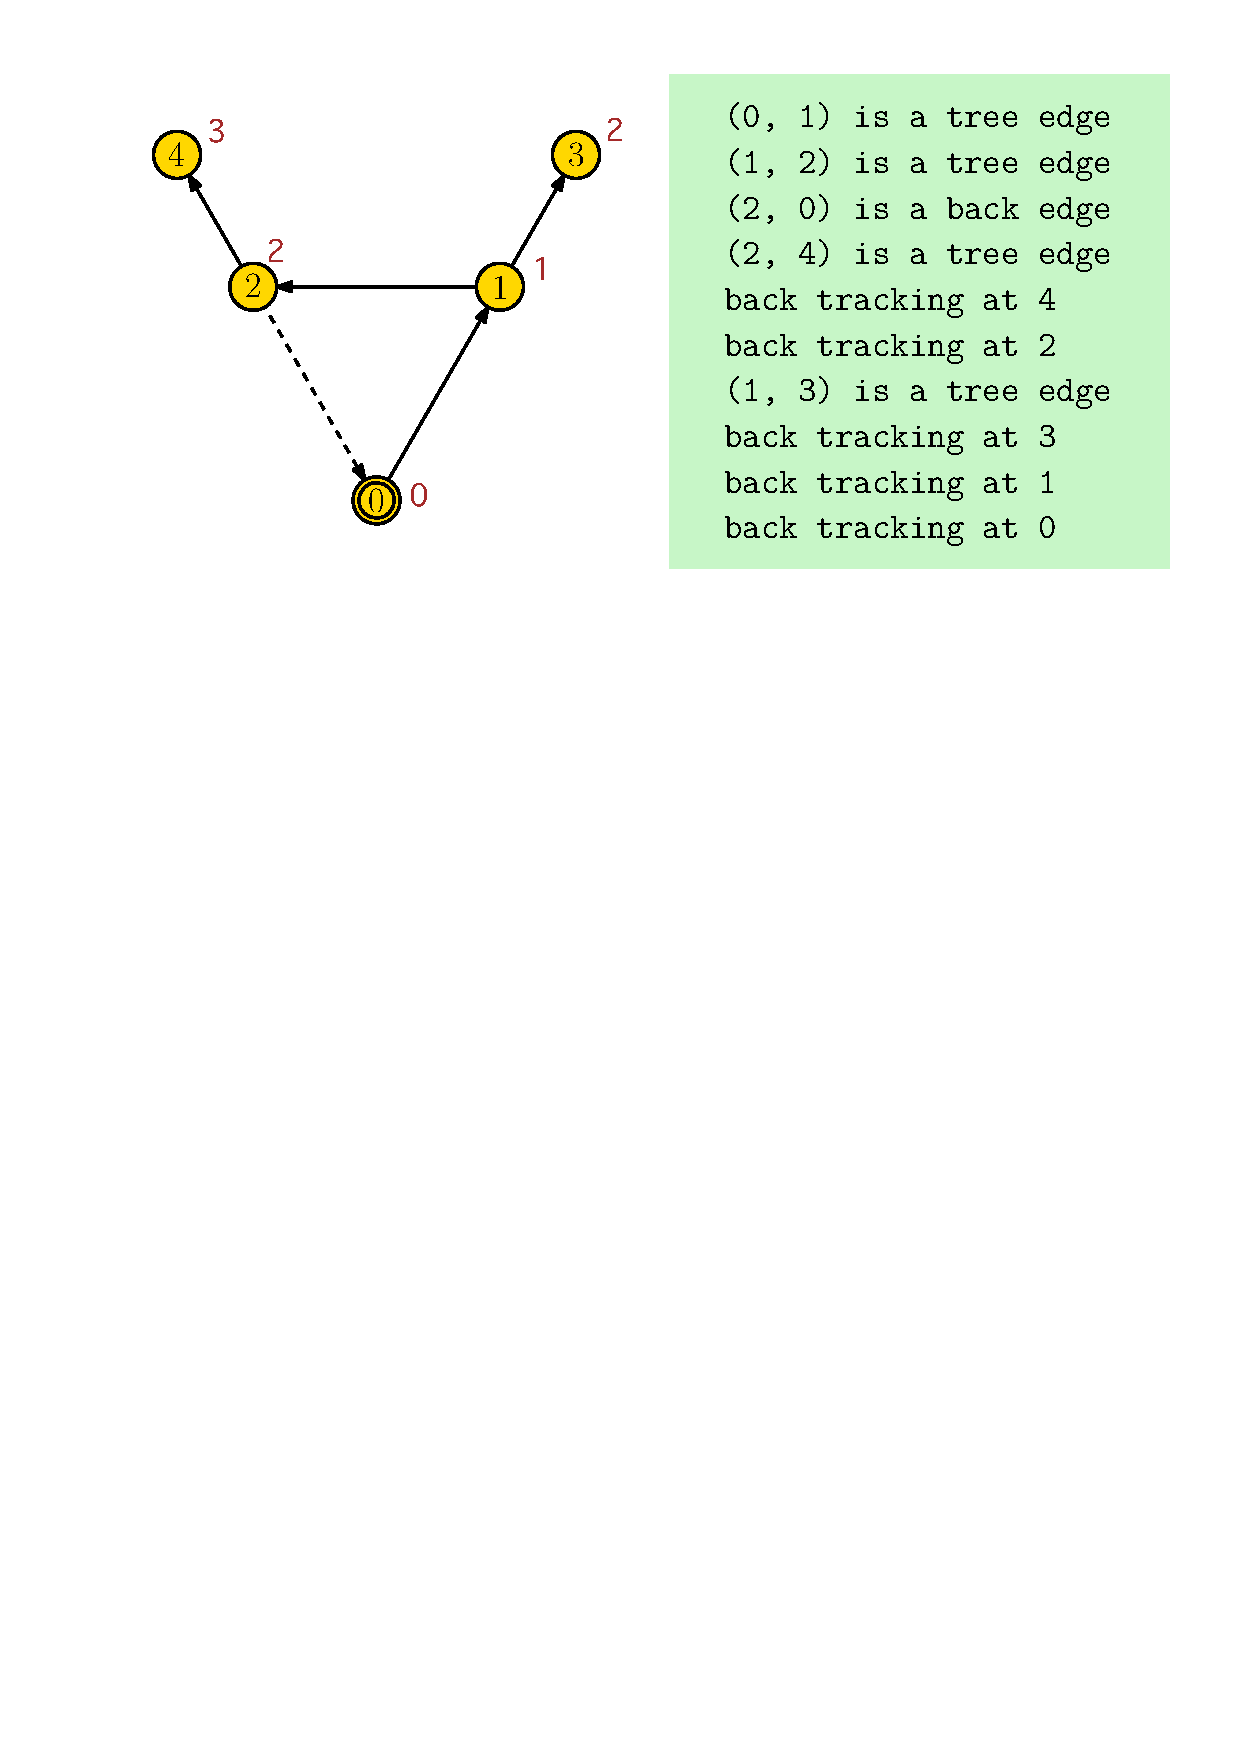
\includegraphics[width=0.39\textwidth]{figures/dfs_bull.pdf}
\end{figure}
\end{paracol}

\vspace*{-0.5\intextsep}
右図は雄牛グラフに対して頂点$0$を根として深さ優先探索を実行した例である。
実線矢印は木辺で破線矢印は補木辺。添字は深さ優先探索木における根までのパスの長さを表す。
また\lstrefname\ref{lst:dfs_back_track}の実行結果も緑の枠内に示している。







\subsection{深さ優先探索木の性質}


%\vspace{-1\intextsep}
\paragraph{深さ優先探索木上の高さと半順序}
各頂点$v$に関して深さ優先探索木${\mathcal T}$における高さ$h(v)$を
根から$v$までの${\mathcal T}$上の経路の長さとする。
${\mathcal T}$は木なのでどの二頂点間にも唯一の経路が存在する。
%\figurename\ref{fig:dfs_tree_icosahedral}では頂点$0$の高さは根なので$h(0)=0$。
上図の雄牛グラフの深さ優先探索木の例では頂点$0$の高さは根なので$h(0)=0$。
頂点$2$は根と隣接しているが${\mathcal T}$上の経路を考えるので$h(2)=2$。


\setcolumnwidth{0.8\textwidth, 0.2\textwidth}
\begin{paracol}{2}

任意の二頂点$x, y \in V$に関して${\mathcal T}$上の半順序$\preceq$を定義する。
$x \preceq y$で$x$が根から$y$までのパスに含まれることを表す。
反射律、反対称律、推移律を満たすことは容易に確認できる。
%半順序なので、\figurename\ref{fig:dfs_tree_icosahedral}の頂点$1$と頂点$3$のように
半順序なので右図の頂点$u$と頂点$v$のように
比較不能な頂点対が存在することを許す。



\paragraph{先祖と子孫}
この半順序関係に従って先祖と子孫の関係が定義できる。
$x \prec y$なら$x$は$y$の先祖。
$x \succ y$なら$x$は$y$の子孫。
${\mathcal T}_v$で
頂点$v$を根とし$v$と$v$の子孫から誘導される${\mathcal T}$の部分木を表す。
また、ある頂点$v$に対して、$v$から出て行く木辺の集合を$\omega^+(v)$で表す。
同様に$\omega^-(v)$で$v$から出て行く補木辺の集合とする。
例えば右図でいうと木辺$(x, y)$に対して$\omega^+(y)=\{(y, u), (y, v), (y, w)\}$であり、
$\omega^-(y)=\{(y, a), (y, b)\}$である。



\switchcolumn
\vspace{.5\intextsep}
\centering
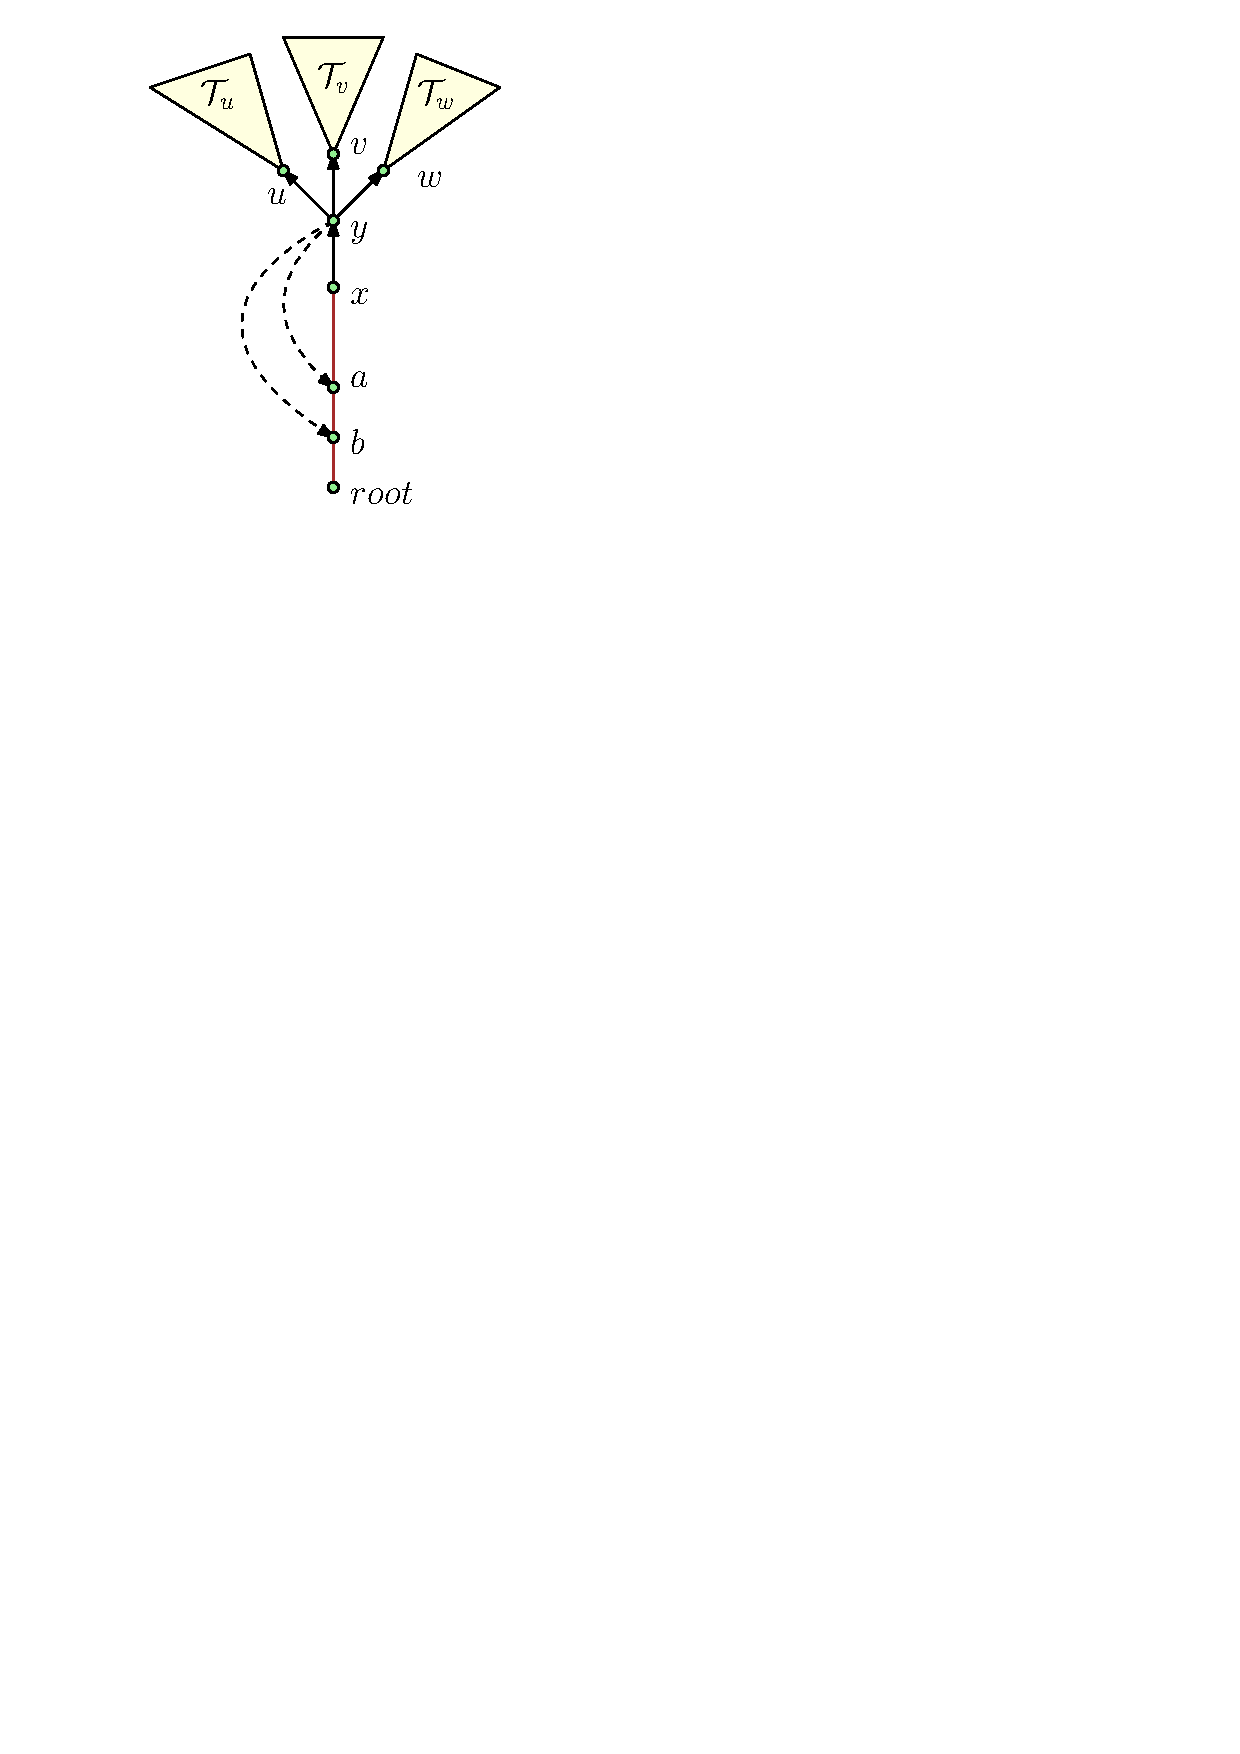
\includegraphics[width=0.18\textwidth]{figures/omegas.pdf}
\end{paracol}




%\vspace*{-0.7\intextsep}
\setcolumnwidth{0.75\textwidth, 0.25\textwidth}
\begin{paracol}{2}

\paragraph{深さ優先探索順序}
深さ優先探索に基づく頂点の遷移順序を定式化する。
$G=(V, E)$を$n$頂点の連結グラフとする。
$\sigma=(v_1, \ldots, v_n)$を$V$上の任意の置換とし、
$\sigma_i$で$i$番目までの部分列を表す。
頂点$v \in V \setminus \sigma_i$に関して
$\nu_{\sigma_i}(v)$で$\sigma_i$内に存在する$v$の隣接頂点の最後方の位置を表す。
$\sigma_i$内に隣接頂点が存在しない場合は$\nu_{\sigma_i}(v)=0$。
このとき次の条件を満たす$\sigma$を深さ優先探索順序という。
すべての$1 < i \leq n$に関して、
$\nu_{\sigma_{i-1}}(v_i) = \max\limits_{j=i,\ldots,n}\nu_{\sigma_{i-1}}(v_j)$。
%直感的には、$\sigma_i$を木と見做すと$\nu_{\sigma_i}(v)$は$v$と接続できる最近
%発見された頂点の$\sigma$上の位置となる。
%また、条件式で$\max$をとっているのは探索の最先端を意図する。

右図に対応する深さ優先順序として、例えば
$(0,11,10,9,8,7,2,6,5,4,3,1)$が得られる。
$i=5$のとき$\sigma_i=(0, 11,10,9,8)$であり、
$\nu_{\sigma_i}(7)=5$となる。%$\nu_{\sigma_i}(4)=3$。
頂点$7$は$\sigma_i$内のすべての頂点と隣接するが、
最後方の頂点$8$の位置$5$をとる。
頂点$6$は$\sigma_i$のどの頂点とも隣接しないので$\nu_{\sigma_i}(6)=0$。
また、$\sigma_i$に無い頂点$1,2,7$が$8$と隣接するので、
$\nu_{\sigma_{i}}(1) = 
\nu_{\sigma_{i}}(2) = 
\nu_{\sigma_{i}}(7) = 
\max\limits_{j=i,\ldots,n}\nu_{\sigma_{i}}(v_j)$。
このとき頂点$1, 2, 7$のいずれの選択も許されるが、
結果として得られる深さ優先探索木の構造は異なる可能性がある。

\switchcolumn
\vspace*{.5\intextsep}
%\begin{figure}[ht]
\centering
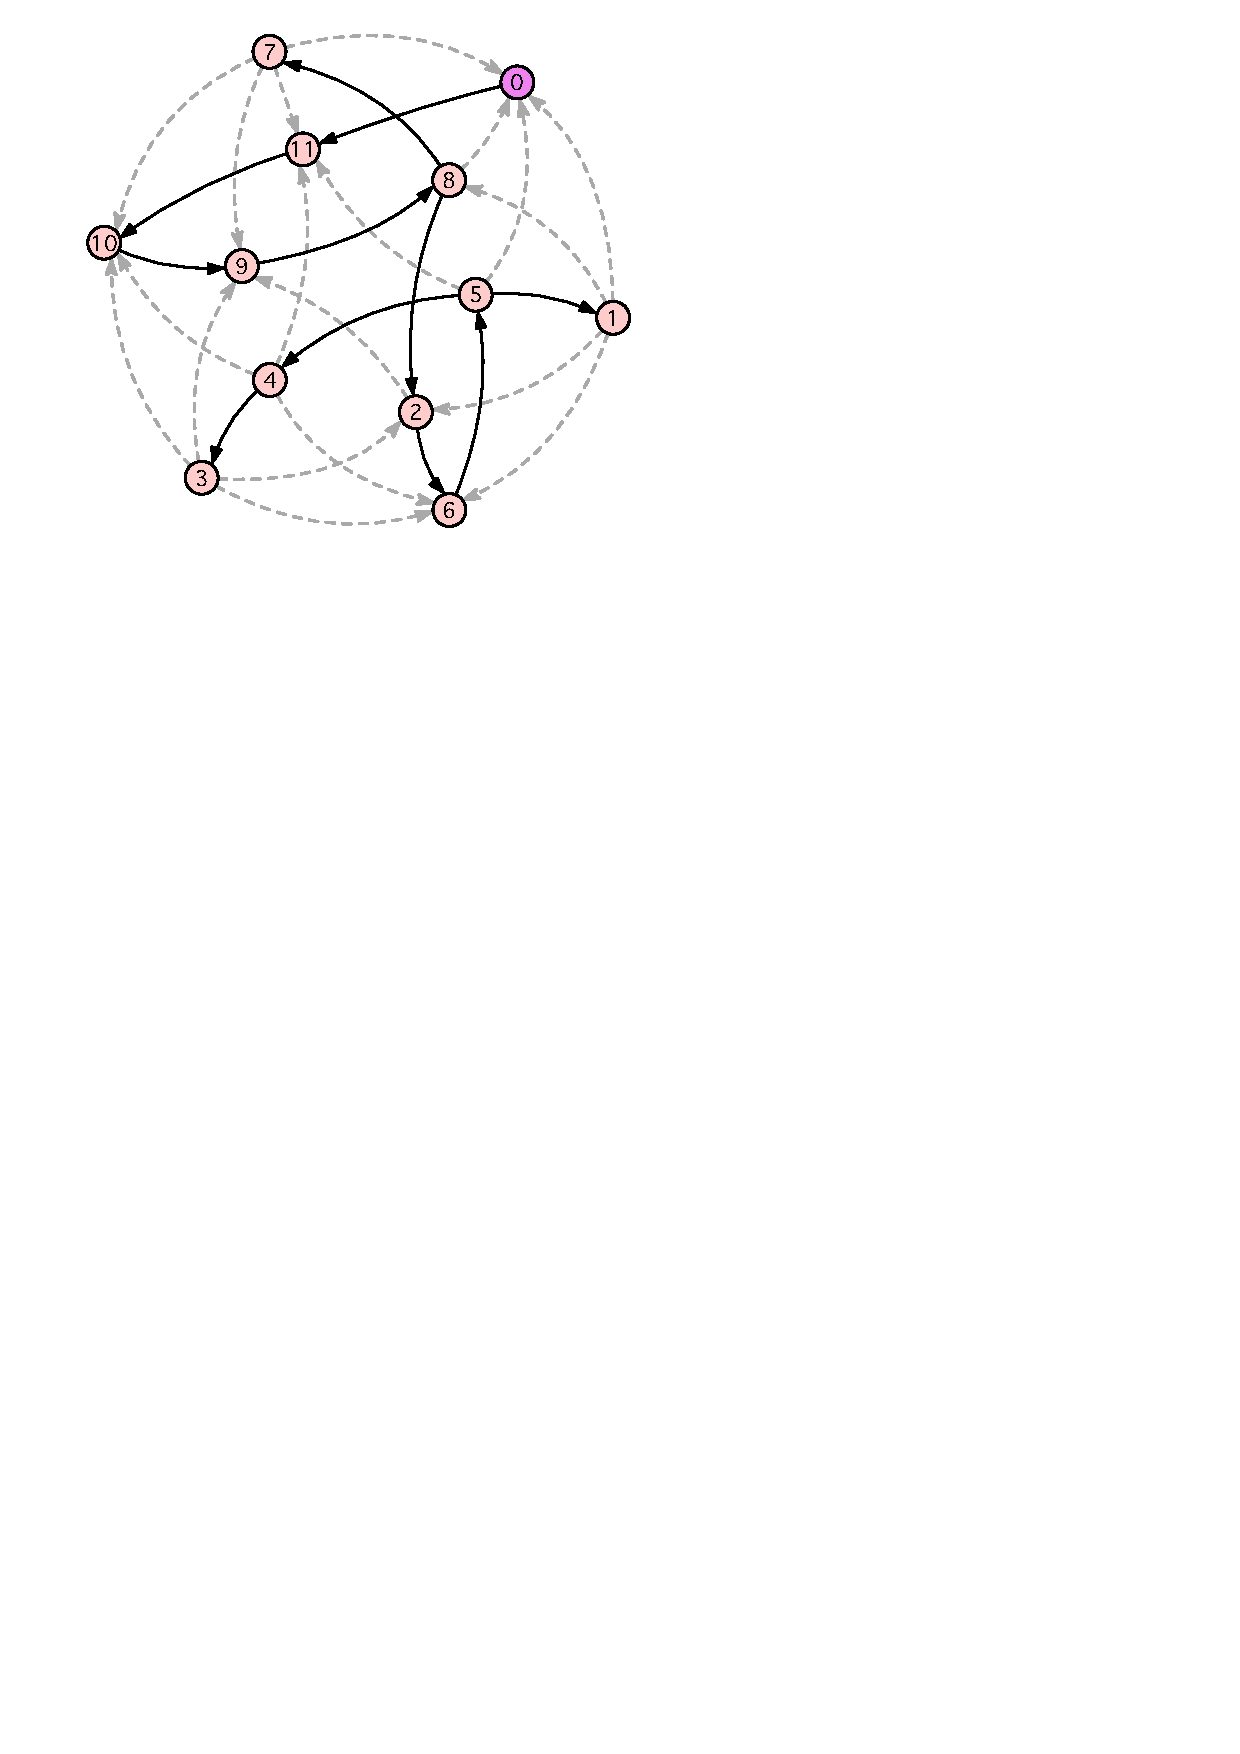
\includegraphics[width=0.23\textwidth]{figures/dfs_icosahedral.pdf}\\
{\small 十二面体グラフの\\深さ優先探索木}
%\caption{{\small 十二面体グラフの深さ優先探索木の例}}
%\label{fig:dfs_tree_icosahedral}
%\end{figure}
\end{paracol}


\begin{lemma}
\label{lemma:dfs_ordering}
連結グラフ$G=(V, E)$とその深さ優先探索木${\mathcal T}=(V, T)$において、
任意の補木辺$(x, y) \in E \setminus T$は$x\succeq y$を満たす。
\end{lemma}


\setcolumnwidth{0.8\textwidth, 0.2\textwidth}
\begin{paracol}{2}
\begin{proof}
$x \preceq y$なる補木辺$(x, y)$が存在すると仮定すると
深さ優先探索順序の条件式に矛盾する。

比較不能な頂点$x,y$間を接続する補木辺$(x,y)$が存在すると仮定する。
このとき$x\in {\mathcal T}_w$および$y \in {\mathcal T}_v$となる
頂点$u$および木辺対$(u, v), (u, w) \in \omega^+(u)$が存在する。
一般性を失うことなく、
${\mathcal T}$の深さ優先探索順序$\sigma$において$v$の方が$w$より前に現れるとする。
%$\omega^+(u)$の他の木辺の終点は$v$と$w$の間には現れないとする。
%$\sigma$において${\mathcal T}_v$の頂点の方が
%${\mathcal T}_w$の頂点より先に現れる。
%このとき$x$は$y$より先に発見されているので、
%$x, y$はそれぞれ${\mathcal T}_v, {\mathcal T}_w$の頂点である。
$k$を${\mathcal T}_v$の頂点の個数$-1$とし$\sigma$における$v$の位置を$i$とすると
$\sigma_{i+k}=w$となる。
また、${\mathcal T}_w$ の$w$を除く任意の頂点$x'$は$\nu_{\sigma_{i+k}}(x') = 0$。
しかし$x$と$y$は互いに隣接するので
$\nu_{\sigma_{i+k}}(w) < \nu_{\sigma_{i+k}}(x)$であり、
%深さ優先探索順序の条件式の下で
$x$は$w$より先に発見されなければならない。
帰納的にこれは$(u, w)$が木辺であることに矛盾する。
\end{proof}

\switchcolumn
\vspace{1.\intextsep}
\centering
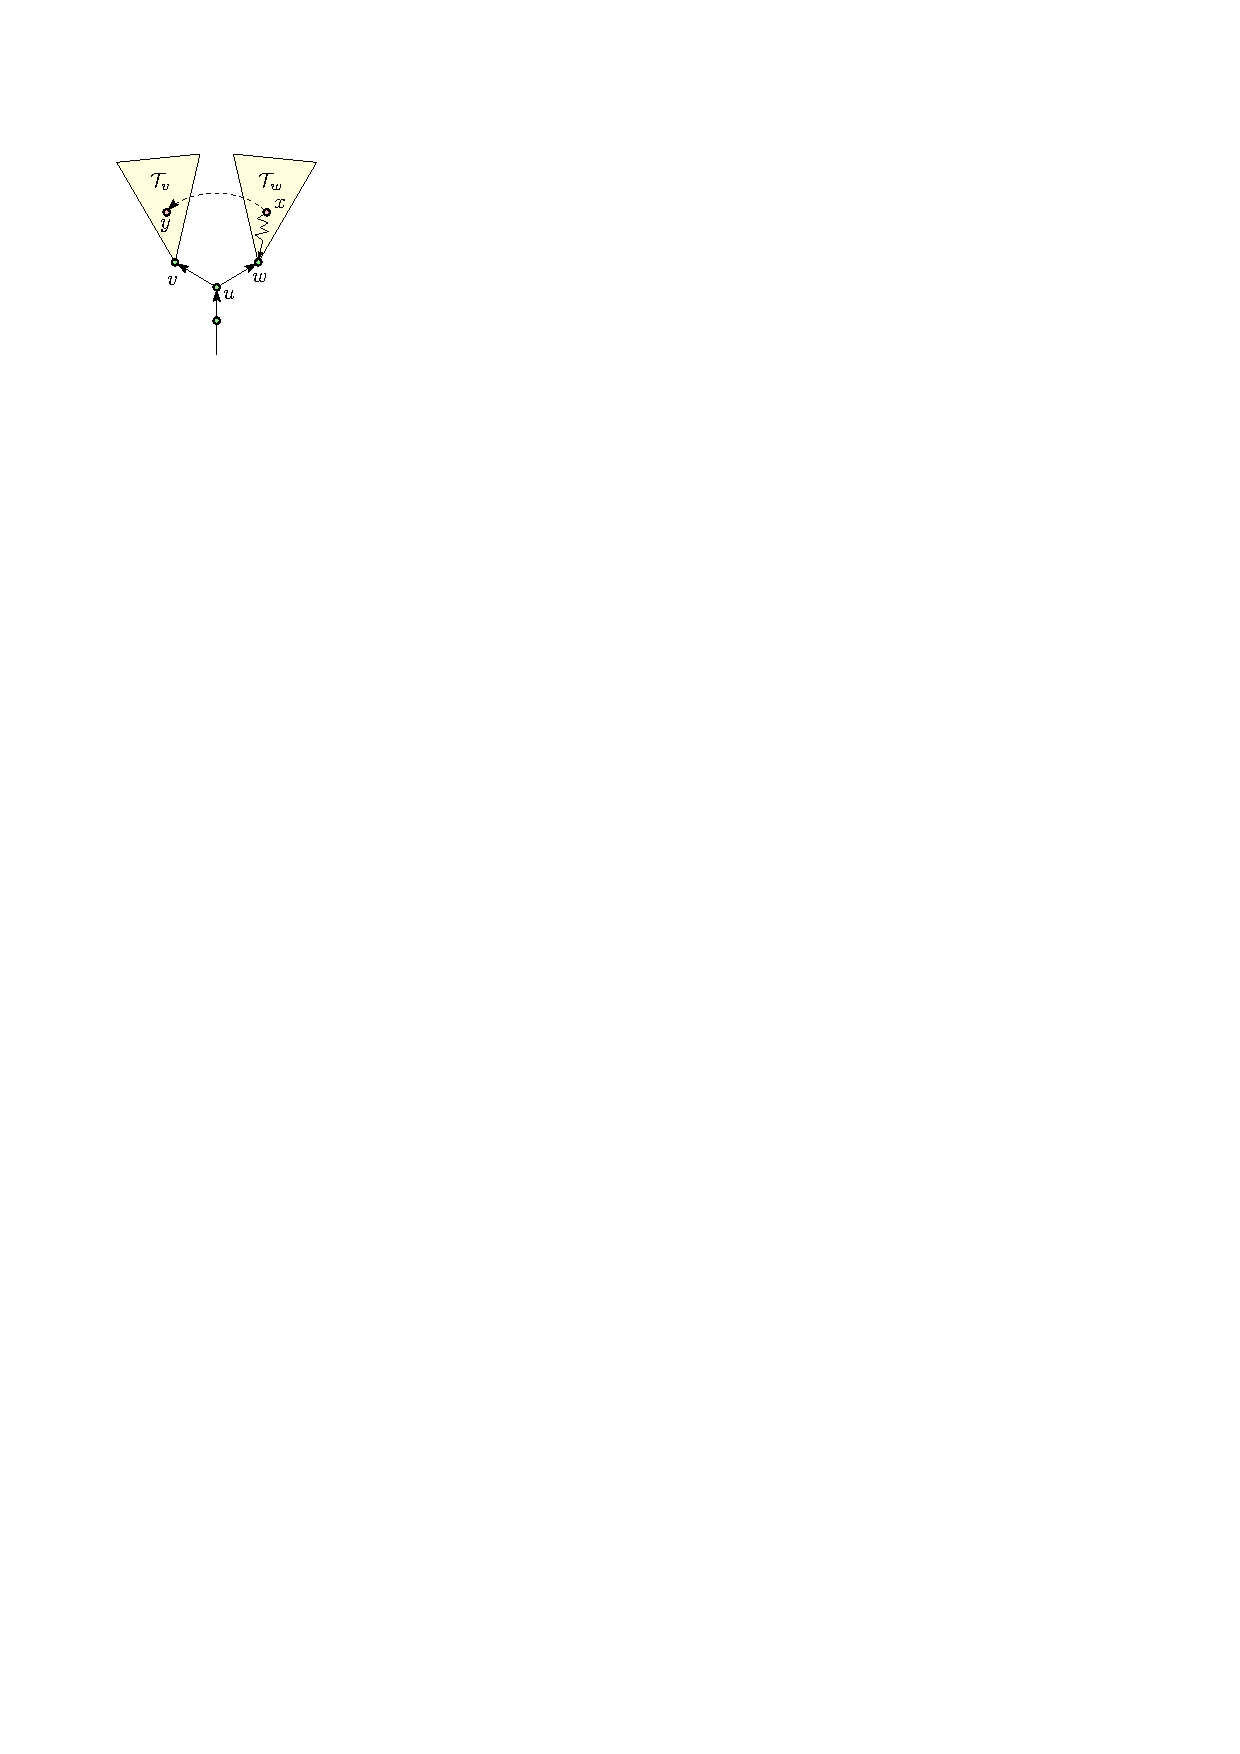
\includegraphics[width=0.19\textwidth]{figures/dfs_ordering2.pdf}
\end{paracol}

%\vspace{-0.5\intextsep}

\paragraph{補木辺の初等閉路}
任意の補木辺$e=(u, v)$は一意に定まる閉路を持つ。
つまり、$v$から$u$への木辺の系列に$e$を結合して得られる有向閉路である。
これを$e$の初等閉路と呼ぶ。
初等閉路の一意性は、
\cref{lemma:dfs_ordering}%深さ優先探索順序の条件式、
および深さ優先探索木${\mathcal T}$上の経路の一意性から導ける。



\setcolumnwidth{0.8\textwidth, 0.2\textwidth}
\begin{paracol}{2}
\paragraph{木辺のフリンジ}
%\cref{lemma:ignoring_back_edges}は、
\cref{lemma:dfs_ordering}により極小な部分問題を
定義づける補木辺の集まりであるフリンジを導入することができる。
深さ優先探索のバックトラックで$T \setminus E$内の探索範囲を限定し、
禁止構造の発見に貢献する補木辺とそれ以外とを区別する。
%注意を払わないといけない補木辺を区別する役割も持つ。


\begin{definition}
連結なグラフ$G=(V, E)$とその深さ優先探索木${\mathcal T}=(V, T)$が与えられたとき、
ある木辺$e = (x, y) \in T$のフリンジを次のように定義する。
\[
\fringe(e) = \{(u, v) \in E \setminus T ~|~ u \succeq y ~\mathrm{and}~ v \preceq x\}.
\]
\end{definition}


\switchcolumn
\vspace{.5\intextsep}
\centering
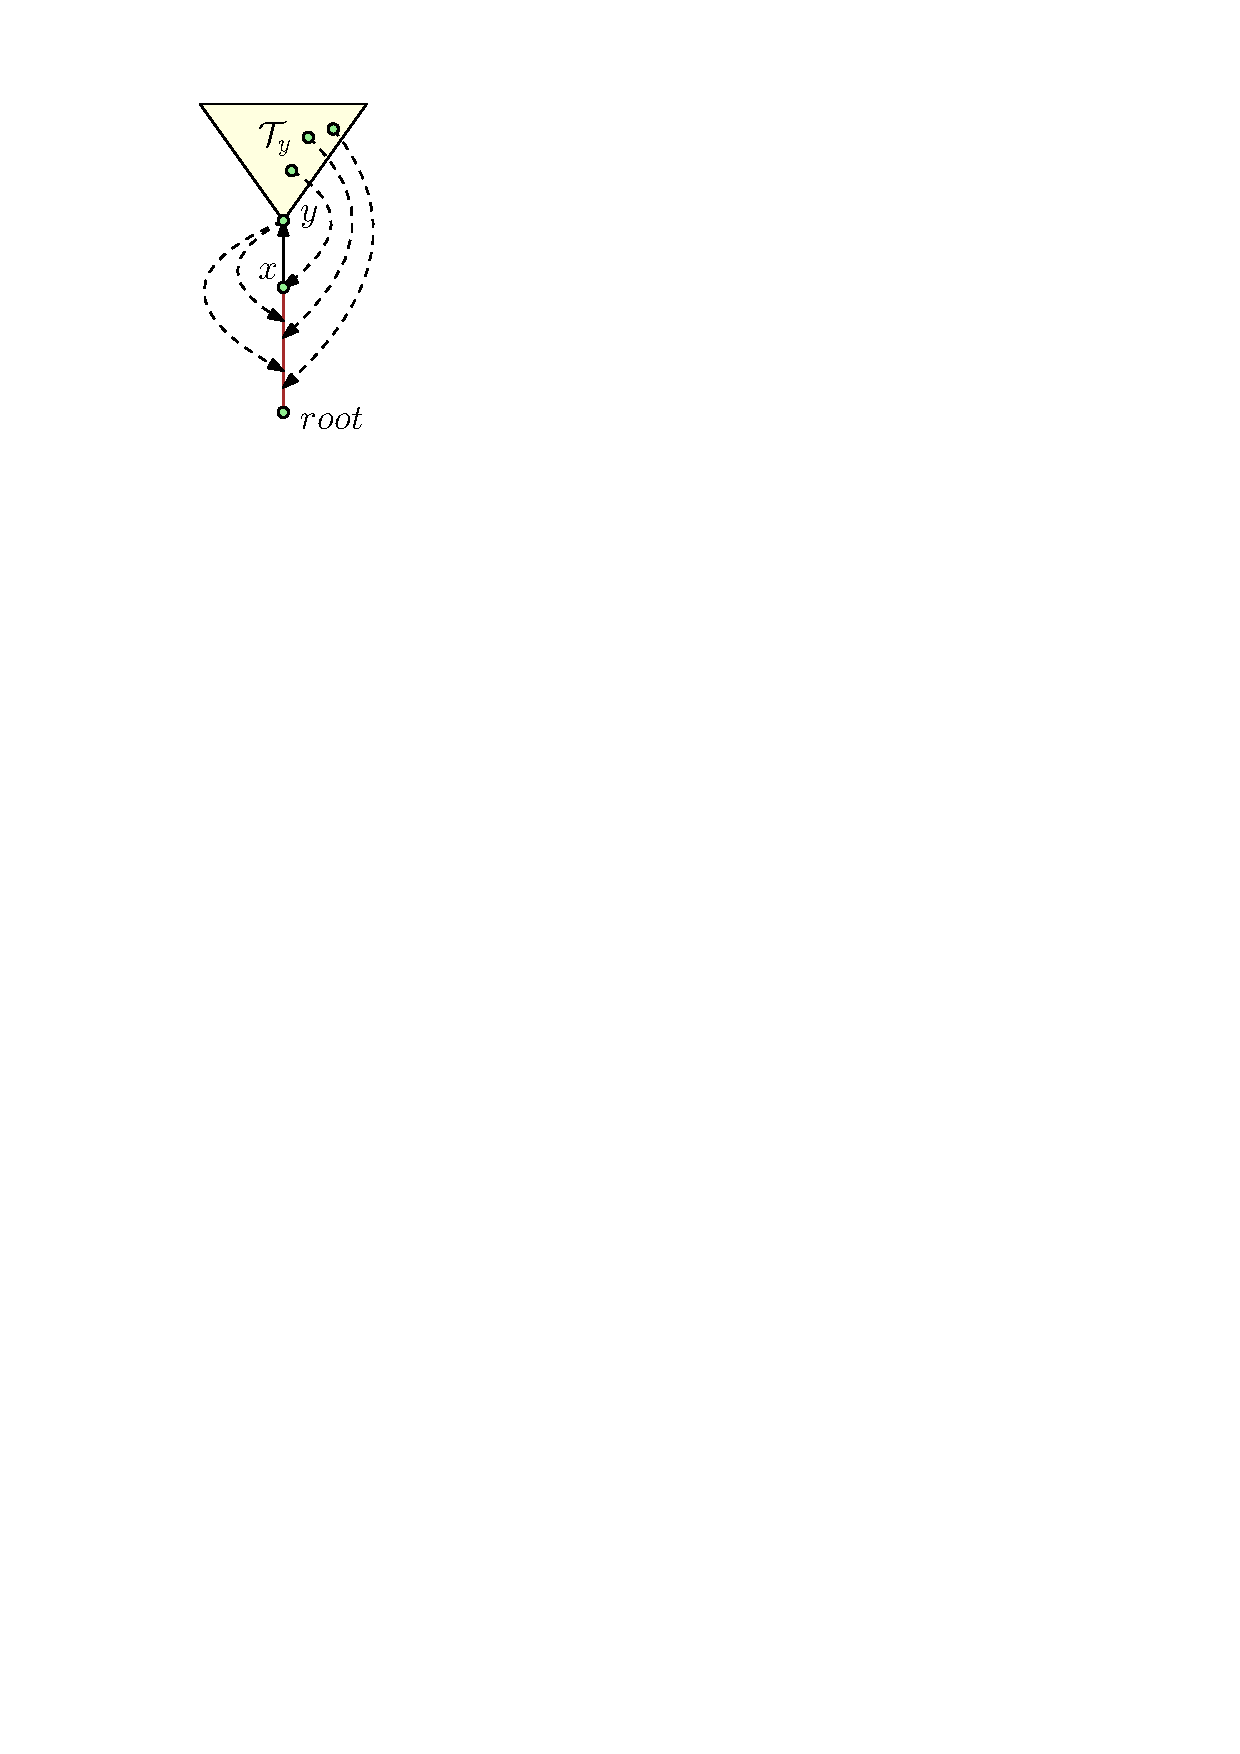
\includegraphics[width=0.1\textwidth]{figures/fringe_image1.pdf}
\end{paracol}

フリンジは対応する木辺$e=(x, y)$の${\mathcal T}_y$に始点を持ち
$y$の先祖に接続する補木辺の集まりである。
木辺$(x, y)$を基準に禁止構造の有無を調べる解法設計においては
$\fringe(e)$に限定できるかをきちんと考察する必要がある。
始点と終点がともに${\mathcal T}_y$にある補木辺の集合
$T_{\succeq y}=\{(u, v) \in E \setminus T ~|~ y \preceq v\}$が
比較対象外にできれば効率は大きく変わる。

%ただし、平面性判定においては補木辺の終点の高さだけでなく視点の高さも禁止構造に
%関係するので判定で用いる位相構造の不変条件には注意が必要である。



\begin{comment}
\begin{lemma}
\label{lemma:ignoring_back_edges}
%グラフ$G=(V, E)$およびその深さ優先探索木${\mathcal T}=(V, T)$に関して、
ある頂点$v$の子孫の部分木${\mathcal T}_v$の辺集合$T_v$および
$T_{\geq h(v)}$が誘導する
部分グラフ$G[T_v \cup T_{\geq h(v)}]$が禁止構造を含まないなら
%すなわち平面的なら
$v$の先祖の判定において$T_{\geq h(v)}$内のすべての補木辺は
比較の対象外として良い。
ただし、位相構造の制約は保持される場合がある。
\end{lemma}

\begin{proof}
\cref{lemma:dfs_ordering}より
$v_1, v_2 \in \omega^+(v)$に関して、
${\mathcal T}_{v_1},~{\mathcal T}_{v_2}$は互いに点素であり辺素である。
禁止構造が存在するとすれば
$\bigcup\limits_{e_i \in \hat{o}(v)} \fringe(e_i) \setminus T_{\geq h(v)}$
内の補木辺の組合せに拠る。
ただし$\hat{o}(v) = \{(v, v_i) ~|~ v_i \in \omega^+(v)\}$。
\end{proof}
\end{comment}


%一意性は深さ優先探索順序の条件式、および${\mathcal T}$上のパスの一意性から導ける。
%一意性は



%\begin{corollary}[子孫の部分木の包含関係と排他性]
%反順序$\succeq$の推移律から$x \preceq y$なら
%${\mathcal T}_y \subseteq {\mathcal T}_x$が成り立つ。
%$(y, u)$と$(y, v)$が始点$y$を共有する木辺であるなら
%${\mathcal T}_u \cap {\mathcal T}_v = \varnothing$が成り立つ。
%これも推移律から${\mathcal T}_u$および${\mathcal T}_v$それぞれの
%任意の部分木間にも排他性が成り立つ。
%\end{corollary}
%半順序$\preceq$は深さ優先探索木に対して重要な特徴付けを与える。
%まず、すべての木辺$(x, y)$は$x \prec y$であり、
%すべての補木辺$(x, y)$は$x \succ y$。
%補木辺が比較不能な頂点どうしを接続しないことは
%深さ優先探索順序の条件式が保証する。









%%%%%%%%%%%%%%%%%%%%%%%%%%%%%%%%%%%%%%%%%%%%%%%%%%%%%%%%%%%%%%%%%%%%%%%%%%%%%%%%%%%%
\subsection{グラフの\texorpdfstring{$2$}-辺連結性}
ここでは深さ優先探索に基づきグラフの構造分析の応用として$2$-辺連結性を判定する
問題を考察する。
特に、\cref{lemma:dfs_ordering}および%\cref{lemma:ignoring_back_edges}
フリンジが定義する極小な部分問題の重要性を確認したい。
グラフの$2$-辺連結性は任意の辺を削除しても連結性を損なわない性質をいう。
別の言い方をすると禁止構造としての橋を持たないグラフである。


%$2$-辺連結性判定のアルゴリズムを記述する前に基本的な事実を確認する。


\begin{lemma}\label{lemma:bridge_is_tree_edge}
橋は木辺。
\end{lemma}
\begin{proof}
補木辺となる橋が存在すると初等閉路の$2$-辺連結性に矛盾。
\end{proof}

\begin{lemma}\label{lemma:no_bridge_has_illegal_cotree_edges}
木辺$e=(x, y)$が橋である必要十分条件は、
%$u \succeq y$および$v \preceq x$を端点とする補木辺$(u, v)$を持たないこと。
$\fringe(e)=\varnothing$であること。
\end{lemma}
\begin{proof}
必要性は背理法で。
主張の前提を満たす補木辺$f\in\fringe(e)$が存在すると仮定すると$f$の初等閉路は$e$を含む。
%\cref{lemma:bridge_is_tree_edge}より、$e$は$f$初等閉路の構成要素なので矛盾。
十分性は演繹的に。
${\mathcal T}_y$の頂点を始点として持たない補木辺は初等閉路内に$e$を含まない。
終点を${\mathcal T}_y$内に持たない場合、
%深さ優先探索順序の条件式より
\cref{lemma:dfs_ordering}は
$y$が根から$x$までのパス上に存在することを保証する。
%同様に両端点を$x$の子孫に持つ補木辺の初等閉路も$e$を含まない。
%$x$の子孫を始点として$x$の子孫でも$y$の先祖でない頂点に接続する補木辺は、
%深さ優先探索の性質上存在しない。
\end{proof}

%\begin{corollary}\label{coro:not_bridge}
任意の補木辺$e=(x, y)$に関して、根から$x$への木辺の系列のうち
頂点$y$以降の各木辺は橋ではない。
従って$\fringe(e)$内の補木辺の終点の高さの最小値
$\min\limits_{(u, v)\in\fringe(e)} h(v)$を適切に管理すれば良い。

%\end{corollary}


\paragraph{$2$-辺連結性判定のpythonコード}
\cref{lemma:no_bridge_has_illegal_cotree_edges}%および
を踏まえると次のような python コードが得られる。
このコードは橋を見つけた時点で$2$-辺連結性を有さないと判定する。
また、\lstrefname\ref{lst:dfs_back_track}との変更箇所を黄緑でハイライトしている。
\begin{lstlisting}[language=Python, caption=$2$-辺連結性判定{\tt has\_bridge},
                   label=lst:dfs_2_edge_connectivity,escapechar=!]
def has_bridge(G, root):
    stack, dfs_height = [(root, iter(G.neighbors(root)))], {x: -1 for x in G}
    dfs_height[root] = 0
    !\hl{lowest = []}!
    while stack:
        parent, children = stack[-1]
        try:
            child = next(children)
            if dfs_height[child] < 0:
                nbr = [x for x in G.neighbors(child) if x is not parent]
                stack.append((child, iter(nbr)))
                dfs_height[child] = dfs_height[parent] + 1
                !\hl{lowest.append([])}!
            else:
                if dfs_height[parent] > dfs_height[child]:
                    !\hl{set\_lower(lowest[-1], dfs\_height[child])}!
        except StopIteration:
            !\hl{child, \_ = stack.pop()}!
            !\hl{\mbox{\textcolor{magenta}{if}} len(lowest) > 0:}!
                !\hl{\mbox{\textcolor{magenta}{if len}}(lowest[-1]) == 0:}!
                    !\hl{\mbox{\textcolor{magenta}{return}} (stack[-1][0], child)}!
                !\hl{prune(lowest, dfs\_height[stack[-1][0]])}!
\end{lstlisting}

\paragraph{コードの簡単な解説}
新たに配列の配列{\tt lowest}を導入し、各木辺$(x, y)$の終点の子孫${\mathcal T}_y$を始点とする
補木辺の終点の高さを管理する。厳密には最も根に近い終点の高さ、つまり高さの最小値を管理する。
橋の検出の場合{\tt lowest}は単純に整数の配列でも用途は足りるが、
後述の平面性判定では${\mathcal T}_y$内の頂点を始点とする複数の補木辺を管理することとなるため
配列の配列として定義している。


\begin{figure}[ht]
    \centering
    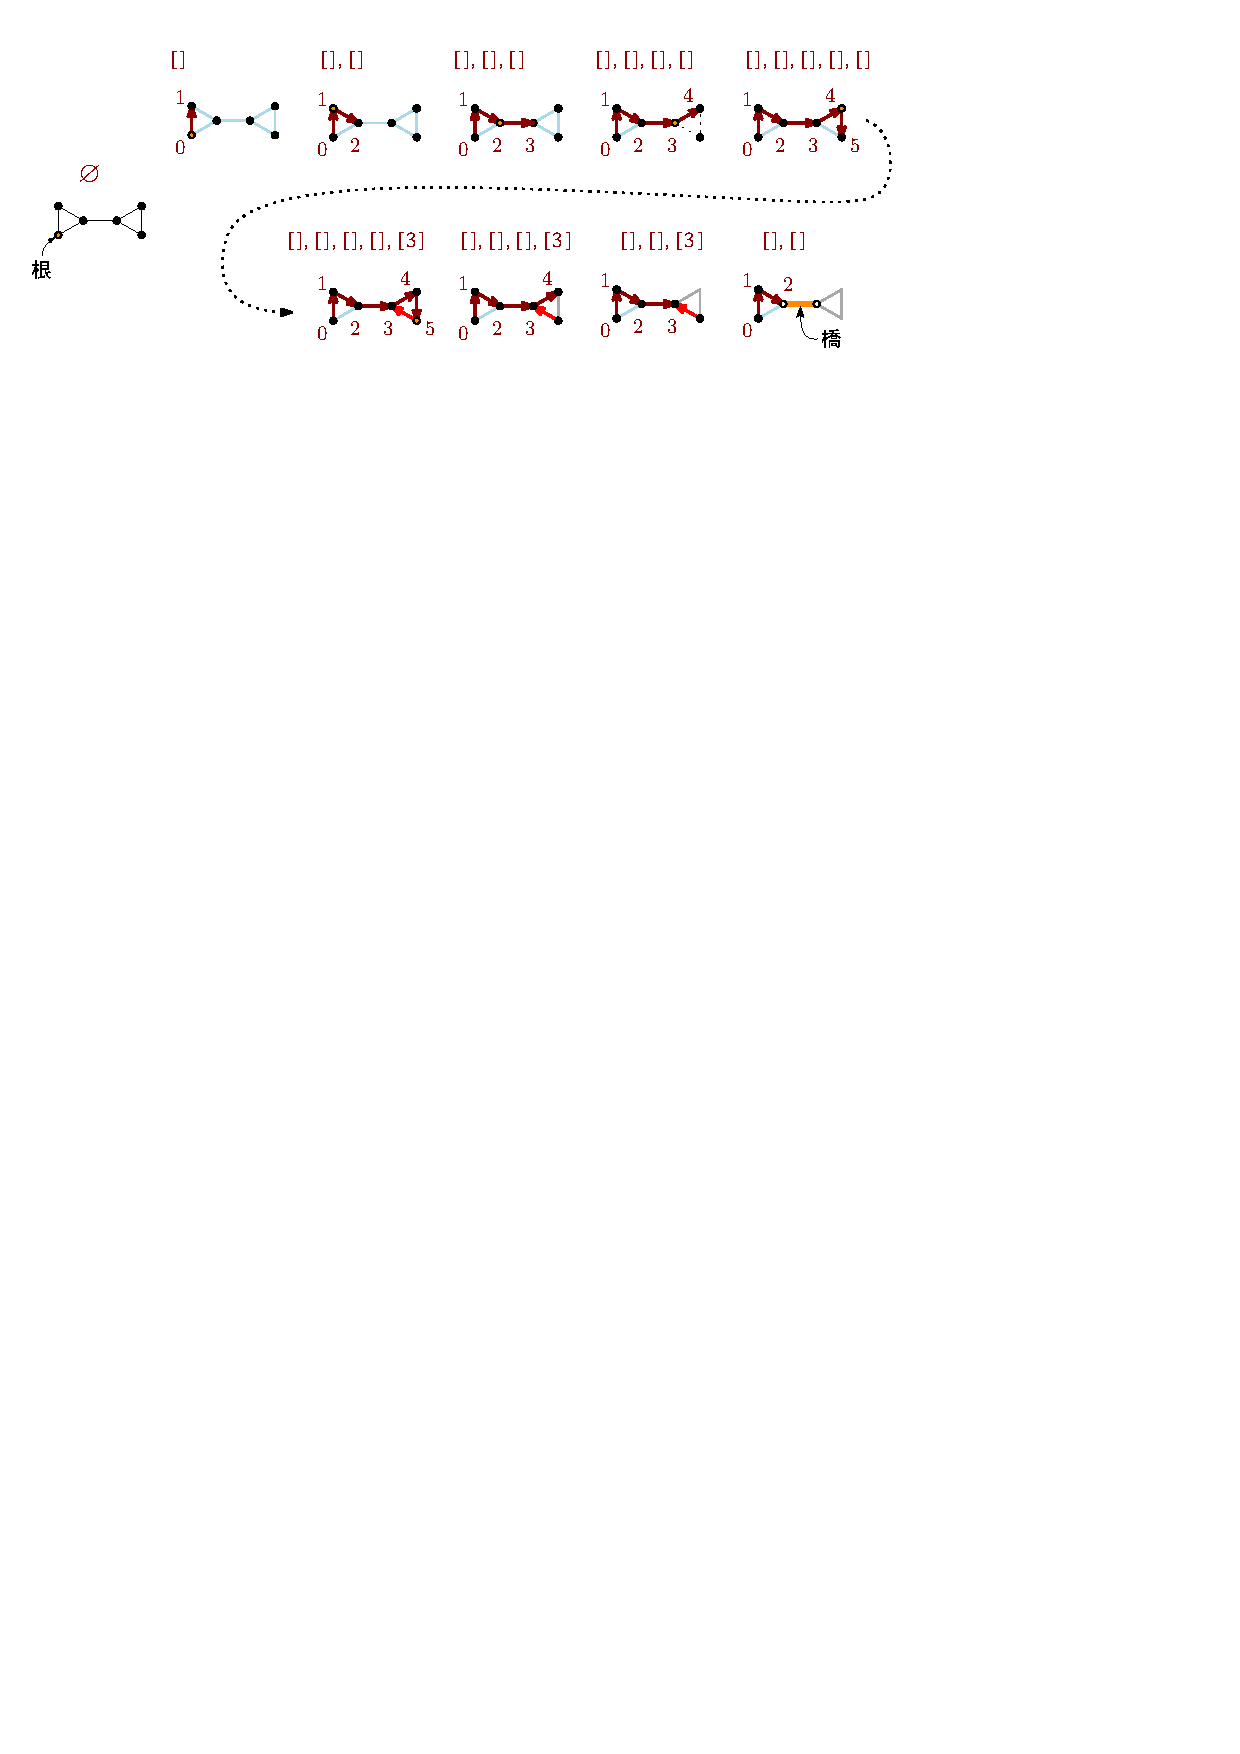
\includegraphics[width=0.95\textwidth]{figures/bridge_illust.pdf}
\end{figure}






探索の初期段階では補木辺は検出されないため空の配列が積み上がっていく(第13行)。
補木辺を見つけたらその終点の高さを{\tt lowest}の末尾の配列に追加する(第16行)。
関数{\tt set\_lower}は対象の配列が空でない場合小さい方を採用する。

橋の具体的な検出はバックトラックで行う。
{\tt lowest}の末尾が空の場合、\cref{lemma:no_bridge_has_illegal_cotree_edges}により
橋が存在すると判定する(第20-21行)。
橋でなかった場合、関数{\tt prune}を用いて先祖の木辺のために補木辺の情報を継承させる。
この際、木辺の終点の高さと{\tt lowest}の末尾の補木辺の終点の高さが等しい場合は継承せずに破棄する。




\lstrefname\ref{lst:dfs_2_edge_connectivity}は二つの
手続き{\tt set\_lower}と{\tt prue}を用いる。
{\tt set\_lower}はより根に近い補木辺の高さを設定する。
引数に{\tt pos}があるのは対象が現行の木辺の更新なのか、
先祖の木辺への更新なのかを切り替えられるよう策定している。
{\tt prune}は不要な補木辺の情報を取り除き、先祖の木辺へ情報を伝播する。
%いずれも簡潔なので解説は省略する。
%これは、\cref{lemma:no_bridge_has_illegal_cotree_edges}に従い
%以降の探索のバックトラックで対象となるいずれの木辺も
%その初等閉路に含まないことを意味する。

\begin{lstlisting}[language=Python, caption=set\_lower,
                   label=lst:set_lower]
def set_lower(pos, h):
    if len(pos) != 0:
        pos[0] = min(pos[0], h)
    else:
        pos.append(h)
\end{lstlisting}

\begin{lstlisting}[language=Python, caption=prune,
                   label=lst:prune_2_edge_connectivity]
def prune(lowest, over_height):
    h = lowest[-1].pop()
    lowest.pop()
    if h < over_height:
        set_lower(lowest[-1], h)
\end{lstlisting}

\paragraph{正当性と計算時間}
アルゴリズムの正当性は
\cref{lemma:no_bridge_has_illegal_cotree_edges}から導ける。
計算量は深さ優先探索と同程度の$O(|E|)$時間で抑えられる。
{\tt stack}の末尾の木辺$(x, y)$に対する最小値更新に係る計算量は、
{\tt set\_lower}を呼び出す回数であり、
頂点$y$から出て行く補木辺の個数に比例するので$O(|\omega^-(y)|)$。
バックトラック時のコストは
%不要な補木辺情報の破棄、および先祖の{\tt lowest}に継承するコスト、
{\tt set\_lower}および{\tt prune}いずれも高々一回呼出しなので$O(1)$となる。
まとめると対象の連結グラフ$G=(V, E)$と
その深さ優先探索木${\mathcal T} = (V, T)$に対して
$\sum\limits_{(x, y) \in T}O(|\omega^-(y)|)+
\sum\limits_{(x, y) \in T}O(1) = O(|E \setminus T|)+O(|T|)=O(|E|)$を得る。




%\subsection{フリンジのデータ構造}
%各木辺に付随するフリンジは平面性判定の極小単位を与える補木辺の部分集合である。
%平面性判定アルゴリズムは、
%各木辺のフリンジ内にクラトフスキー部分グラフの存在確認をそのサイズの線形時間で処理する。
%すべての木辺について調べてクラトフスキー部分グラフが確認できなければ
%対象グラフは平面的であると判定する。


\paragraph{まとめ}
橋でないことを保証するために、各木辺$(x, y)$に対して
$h(x)$と$y$の子孫の補木辺の終点の高さの最小値{\tt lowest}を対応づけ、
一つ一つ健全性を確認しながら進めていく。
バックトラックで子孫の{\tt lowest}を適切に継承し
所望の不変性を維持しつつ({\tt set\_lowest})、
不要な補木辺を破棄する({\tt prune})。
大事なことは監視対象である終点の高さの引き継ぎと適時開放。
これをバックトラック時に適切かつ効率良く処理する手順の設計がとても重要な観点である。

%また、深さ優先探索に基づく構造分析は、
%まず深さ優先探索木があって、木構造は禁止構造ではなく、
%補木辺や初等閉路の組合せによって誘発される禁止構造の特定に
%適するアプローチといえる。

\section{平面性判定アルゴリズム}
まず深さ優先探索に基づく平面性判定の概要を確認する。
次に子孫のフリンジを継承する際に禁止構造を検出する手順を議論する。
禁止構造を検出しなかった場合のアルゴリズムの正当性についても議論する。


%\paragraph{平面性判定と部分問題としてのフリンジ}
\subsection{平面性判定の概要}%と部分問題としてのフリンジ}

\paragraph{平面性判定の概要のpythonコード}
平面性判定アルゴリズムのフレームワークは
\lstrefname\ref{lst:is_planar}に示すように
橋検出の\lstrefname\ref{lst:dfs_2_edge_connectivity}と本質的には変わらない。
入力として連結なグラフ{\tt G}と任意の頂点{\tt root}が与えられたとき、
{\tt G} の{\tt root}から到達可能な連結成分の平面性を判定する。
ハイライトは橋検出との変更箇所を表している。



%変更箇所は各木辺にクラス{\tt fringe}を対応付ける点である。
%木辺$(x, y)$のフリンジを${\mathcal T}_y$の頂点から$y$の先祖に接続するすべての補木辺とする。
%{\tt fringe}はフリンジ内の各補木辺の終点の高さを管理する。

%\hspace{-1.5em}ある木辺のフリンジのイメージは右図のような感じになる。
%破線の補木辺すべてが木辺$(x,y)$のフリンジに属す。




\begin{lstlisting}[language=Python, caption=is\_planar,escapechar=@,
                   label=lst:is_planar]
def is_planar(G, root):
    stack, dfs_height = [(root, iter(G.neighbors(root)))], {x: -1 for x in G}
    dfs_height[root] = 0
    @\hl{fringes}@ = []
    while stack:
        parent, children = dfs_stack[-1]
        try:
            child = next(children)
            if dfs_heights[child] < 0:
                dfs_height[child] = dfs_height[parent] + 1
                stack.append((y, iter([u for u in G.neighbors(child) if u != parent])))
                @\hl{fringes}@.append([])
            else:
                if dfs_height[parent] > dfs_height[child]:
                    @\hl{fringes[-1].append(fringe(dfs\_height[child]))}@
        except StopIteration:
            stack.pop()
            if len(fringes) > 0:
                @\hl{\mbox{\textcolor{magenta}{try}}:}@
                    @\hl{merge\_fringes(fringes, dfs\_height[stack[-1][0]])}@
                @\hl{\mbox{\textcolor{magenta}{except}} Exception:}@
                    @\hl{\mbox{\textcolor{magenta}{return}} False}@
    return True                   
\end{lstlisting}

第20行目の関数{\tt merge\_fringes}が各木辺のフリンジを形成する手続きで、
禁止グラフを検出したら直ちに例外{\tt Exception}を生成し処理を完了する。
直感的には、
スタックの末尾にいる木辺$(x, y)$のフリンジを形成するために、
%終点$y$に接続している子孫の
$\omega^+(y)$内の各木辺のフリンジを継承し併合することを試みる。



\setcolumnwidth{0.6\textwidth, 0.4\textwidth}
\begin{paracol}{2}
\paragraph{フレームワークの計算量}
フレームワークの計算量が、
条件付きで橋検出と同様に深さ優先探索に準ずる計算量$O(|E|)$となることを確認する。
対象グラフ$G=(V, E)$およびその深さ優先探索木${\mathcal T}=(V, T)$とする。
異なる点は第15・20行目の{\tt fringe}周りの処理である。
第15行はただ一つの補木辺で初期化されるフリンジを生成してスタックに積むだけなので$O(1)$。
全体で$O(|E\setminus T|)$。
第20行はスタックの先頭にある木辺$e=(x, y)$の
$O(|\omega^+(y)|)$個の子孫のフリンジと
$O(|\omega^-(y)|)$個のただ一つの補木辺で構成されるフリンジ
を併合して$\fringe(e)$を形成する。

このとき関数{\tt merge\_fringes}が
$O(|\omega^+(y)|+|\omega^-(y)|)$時間で処理できれば
全体で見ても$O(|E|)$で抑えられる。つまり、\\
$\sum_{(x, y) \in T}O(|\omega^+(y)|+|\omega^-(y)|)=
O(|T|)+O(|E\setminus T|)=O(|E|)$。



\switchcolumn
%\vspace{-0.5em}
\vspace{1.5\intextsep}
\begin{figure}[ht]
\centering
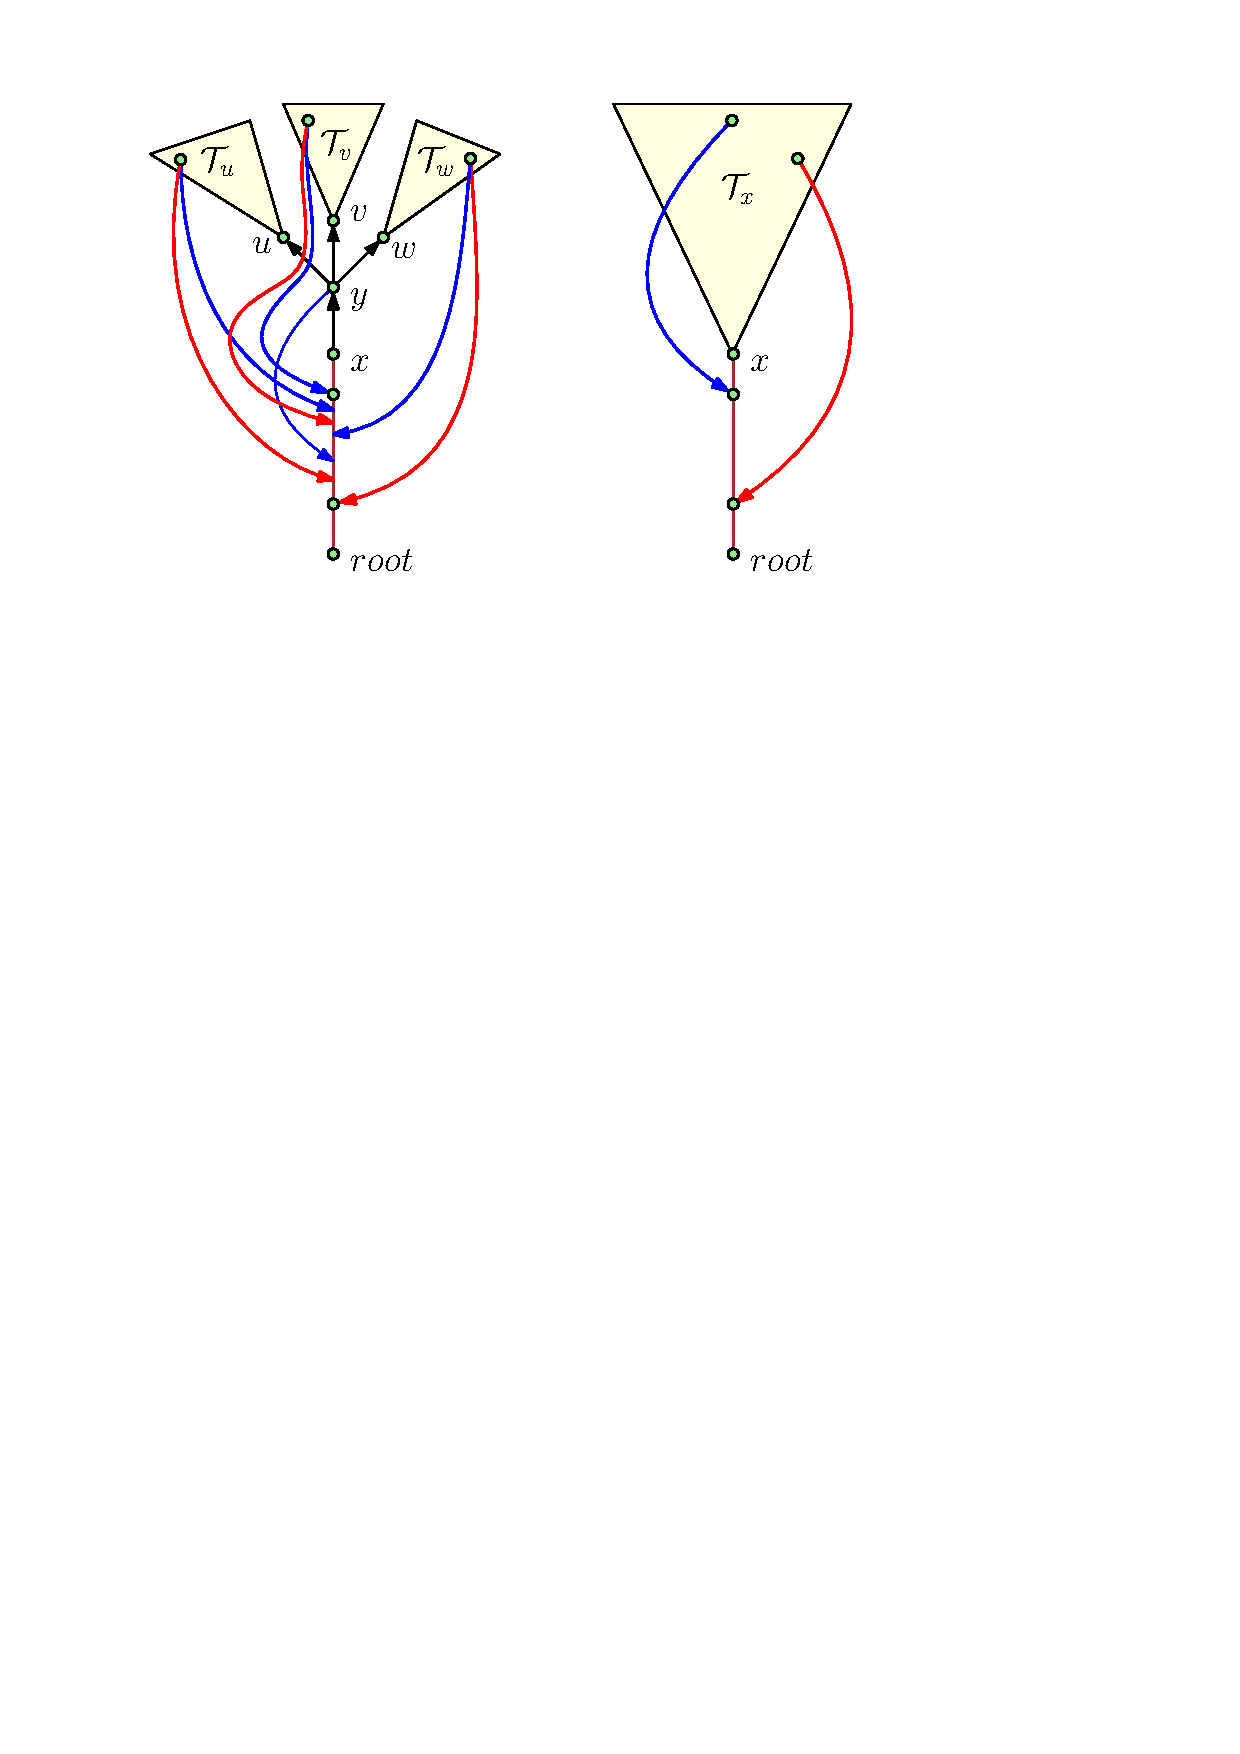
\includegraphics[width=0.39\textwidth]{figures/merging_upper_fringes.pdf}
\end{figure}
\end{paracol}

後述するが、各木辺のフリンジは最も根に近い終点の高さと、
最も根から離れた終点の高さの二つの参照点を備えるだけで十分である。
一つしか補木辺を持たない場合は、それぞれ同じ補木辺を参照する。
二つの子孫間のフリンジの併合は四つの補木辺の終点の高さの比較が主となる。


\setcolumnwidth{0.75\textwidth, 0.25\textwidth}
\begin{paracol}{2}
\paragraph{フリンジの併合と禁止構造}
平面性判定アルゴリズムは、
バックトラックごとにフリンジ内の補木辺が禁止グラフである
クラトフスキーグラフを形成するかを調べる。
%橋検出と同様に禁止グラフを見つけたら、非平面的と判定し処理を完了する。
すべての木辺のフリンジを調べ終わり禁止グラフを検出できなかったら平面的と判定する。

右図は禁止グラフ$K_{3,3}$の細分を含むフリンジの例である。
左は木辺$(x,y)$のフリンジを赤とシアンの矢印の集まりで表している。
各黒辺は木辺とする。右は分かりやすく描画し直した同型のグラフである。
%このようにフリンジは極小な部分問題を定義する重要な役割を果たす。

\switchcolumn
%\begin{figure}[ht]
\vspace{1.\intextsep}
\centering
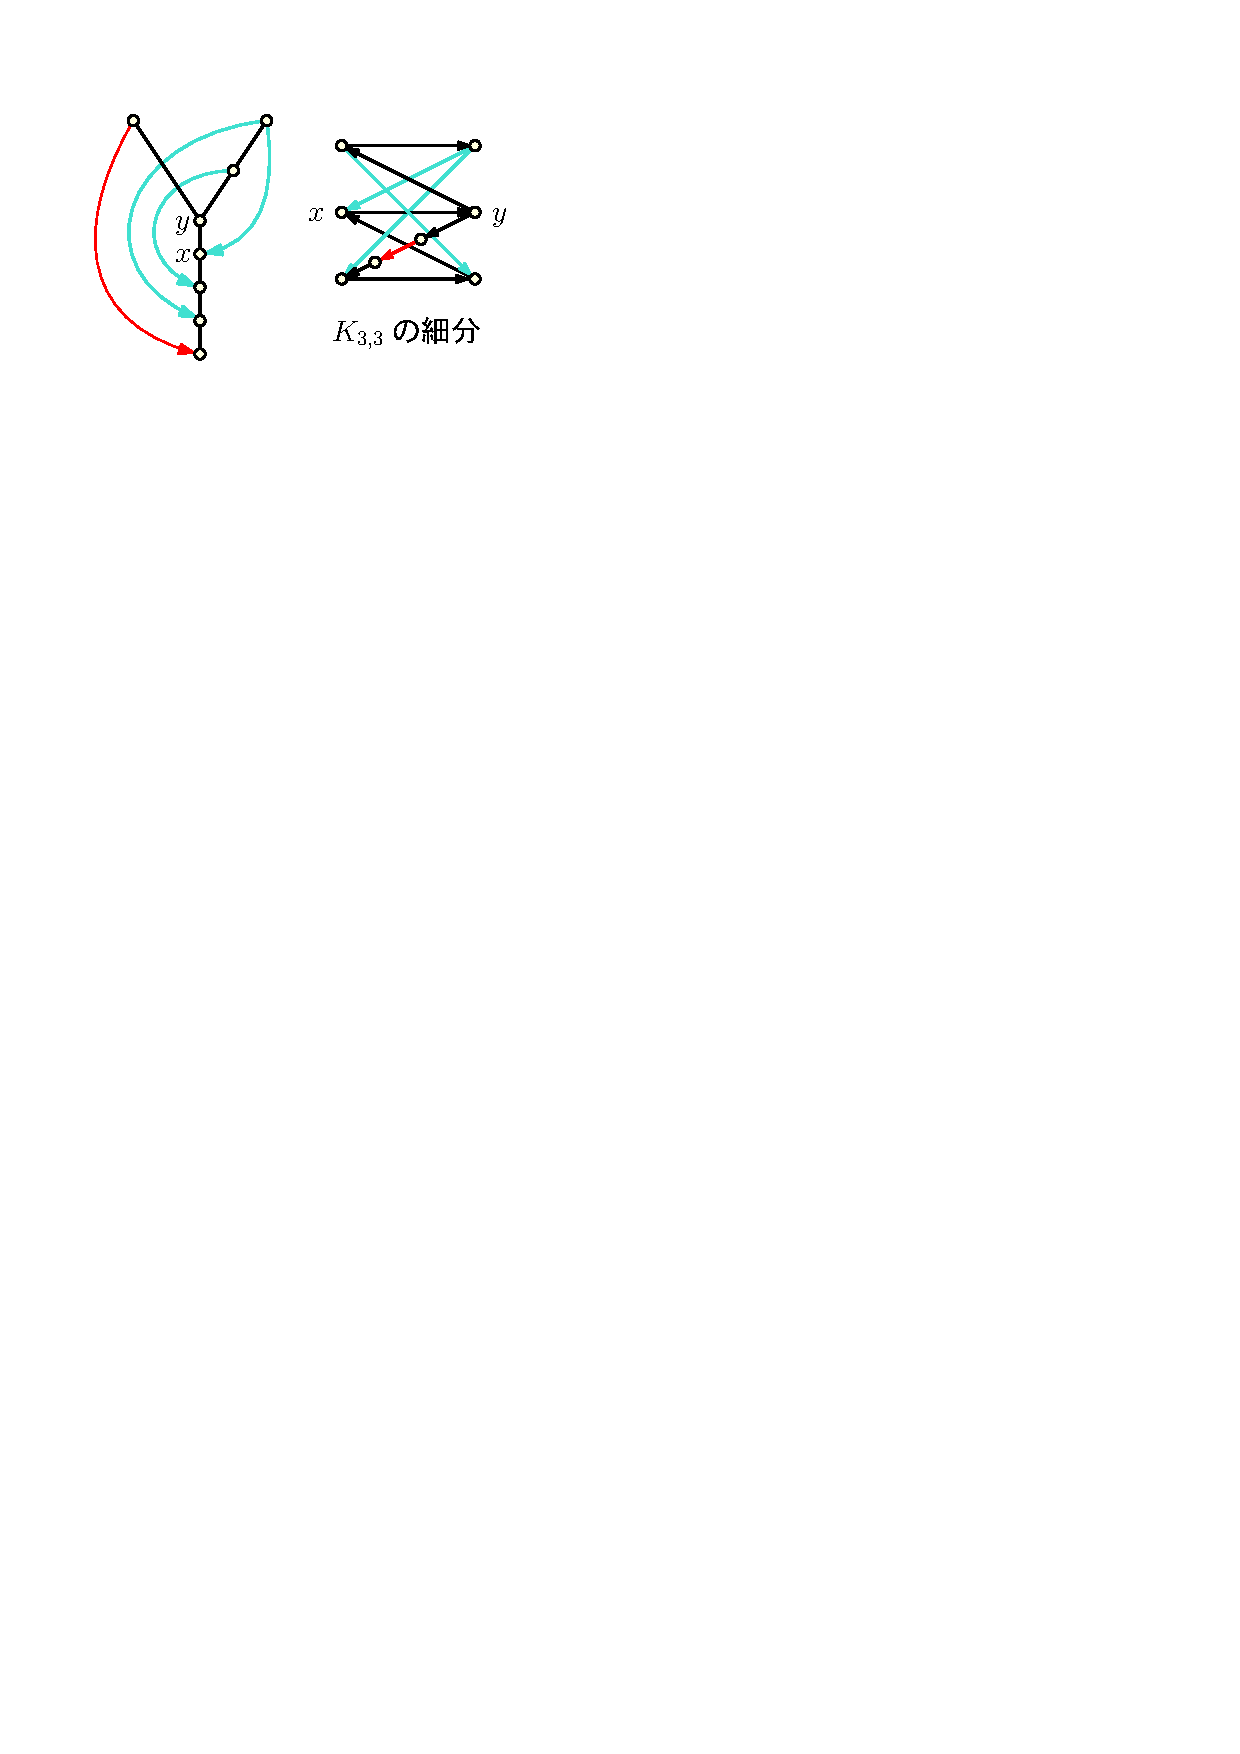
\includegraphics[width=0.24\textwidth]{figures/forbidden_fringe1.pdf}
%\end{figure}
\end{paracol}




\paragraph{継承に基づくフリンジ形成}
%もう少しフリンジの併合の概要が続く。
関数{\tt merge\_fringes}のpythonコードを\lstrefname\ref{lst:merge_fringes}に示す。
関数{\tt get\_merged\_fringes}を用いて
併合したフリンジを取得し(第2行)、
橋検出の場合と同様に不要な補木辺を{\tt fringe}の
クラス関数{\tt prune}を用いて破棄する(第4行)。
%先祖の木辺のフリンジに継承する(第6行)。
第3行の条件式内の{\tt mf is not None}は
$\fringe(e)=\varnothing$で橋の場合の手間を省くための記述である。
第5行の条件式内のクラス変数{\tt fops}は次節で詳説するフリンジ内干渉で
%補木辺の集まりが
極大な非クラフトスキーグラフを見つけるための補木辺の組合せ構造である。
不要な補木辺の破棄で組合せ構造が消滅しない限り先祖のフリンジに継承される(第6行)。

\begin{lstlisting}[language=Python, caption=merge\_fringes,escapechar=@,
                   label=lst:merge_fringes]
def merge_fringes(fringes, dfs_height):
    mf = get_merged_fringe(fringes.pop())
    if mf is not None:
        mf.prune(dfs_height)
        if mf.fops:
            fringes[-1].append(mf)
\end{lstlisting}






\setcolumnwidth{0.66\textwidth, 0.33\textwidth}
\begin{paracol}{2}
\paragraph{フリンジ併合の概要}
\lstrefname\ref{lst:merge_fringes}内で呼ばれる
%関数
{\tt get\_merged\_fringe}は子孫のフリンジリスト
{\tt upper\_fringes}を入力として、
それらを併合したフリンジ{\tt new\_fringe}を出力する。
\lstrefname\ref{lst:get_merged_fringe}はそのpythonコードである。

まず3行目で子孫のフリンジを整列しているが、
各フリンジの最も根に近い補木辺の終点の高さを基準にしている。
右図の例では${\mathcal T}_u < {\mathcal T}_v$となる。
これは根に近い補木辺を持つフリンジほど平面埋込みにおいて
外面に近くあるべきと考えるからである。
第4行以降は、根に近い補木辺を持つものから順に
{\tt fringe}のクラス関数{\tt merge}を用いて併合していく(第5・6行)。

右図は3通りの平面埋込みの例を示しているが、
上段のいずれも最も根に近い補木辺を
持つフリンジの方が外側に来ていることを示している。
下段のように${\mathcal T}_v$の赤線の初等閉路の内側に
${\mathcal T}_u$を埋め込むことはできるが
根も同時に埋め込まなければならず根が外面に現れなくなる。
この状況は後続の処理を複雑にするため好ましくない。
対象グラフが平面的なら
タットのばね\cref{thm:tutte}より
任意の頂点を外面境界上に配置する平面埋込みの存在が保証されるので、
深さ優先探索の根は外面に属す平面埋込みに制限する。
従って下段の平面埋込みは拒否される。



\switchcolumn
%\vspace{-0.5em}
\vspace{1.5\intextsep}
%\begin{figure}[ht]
\centering
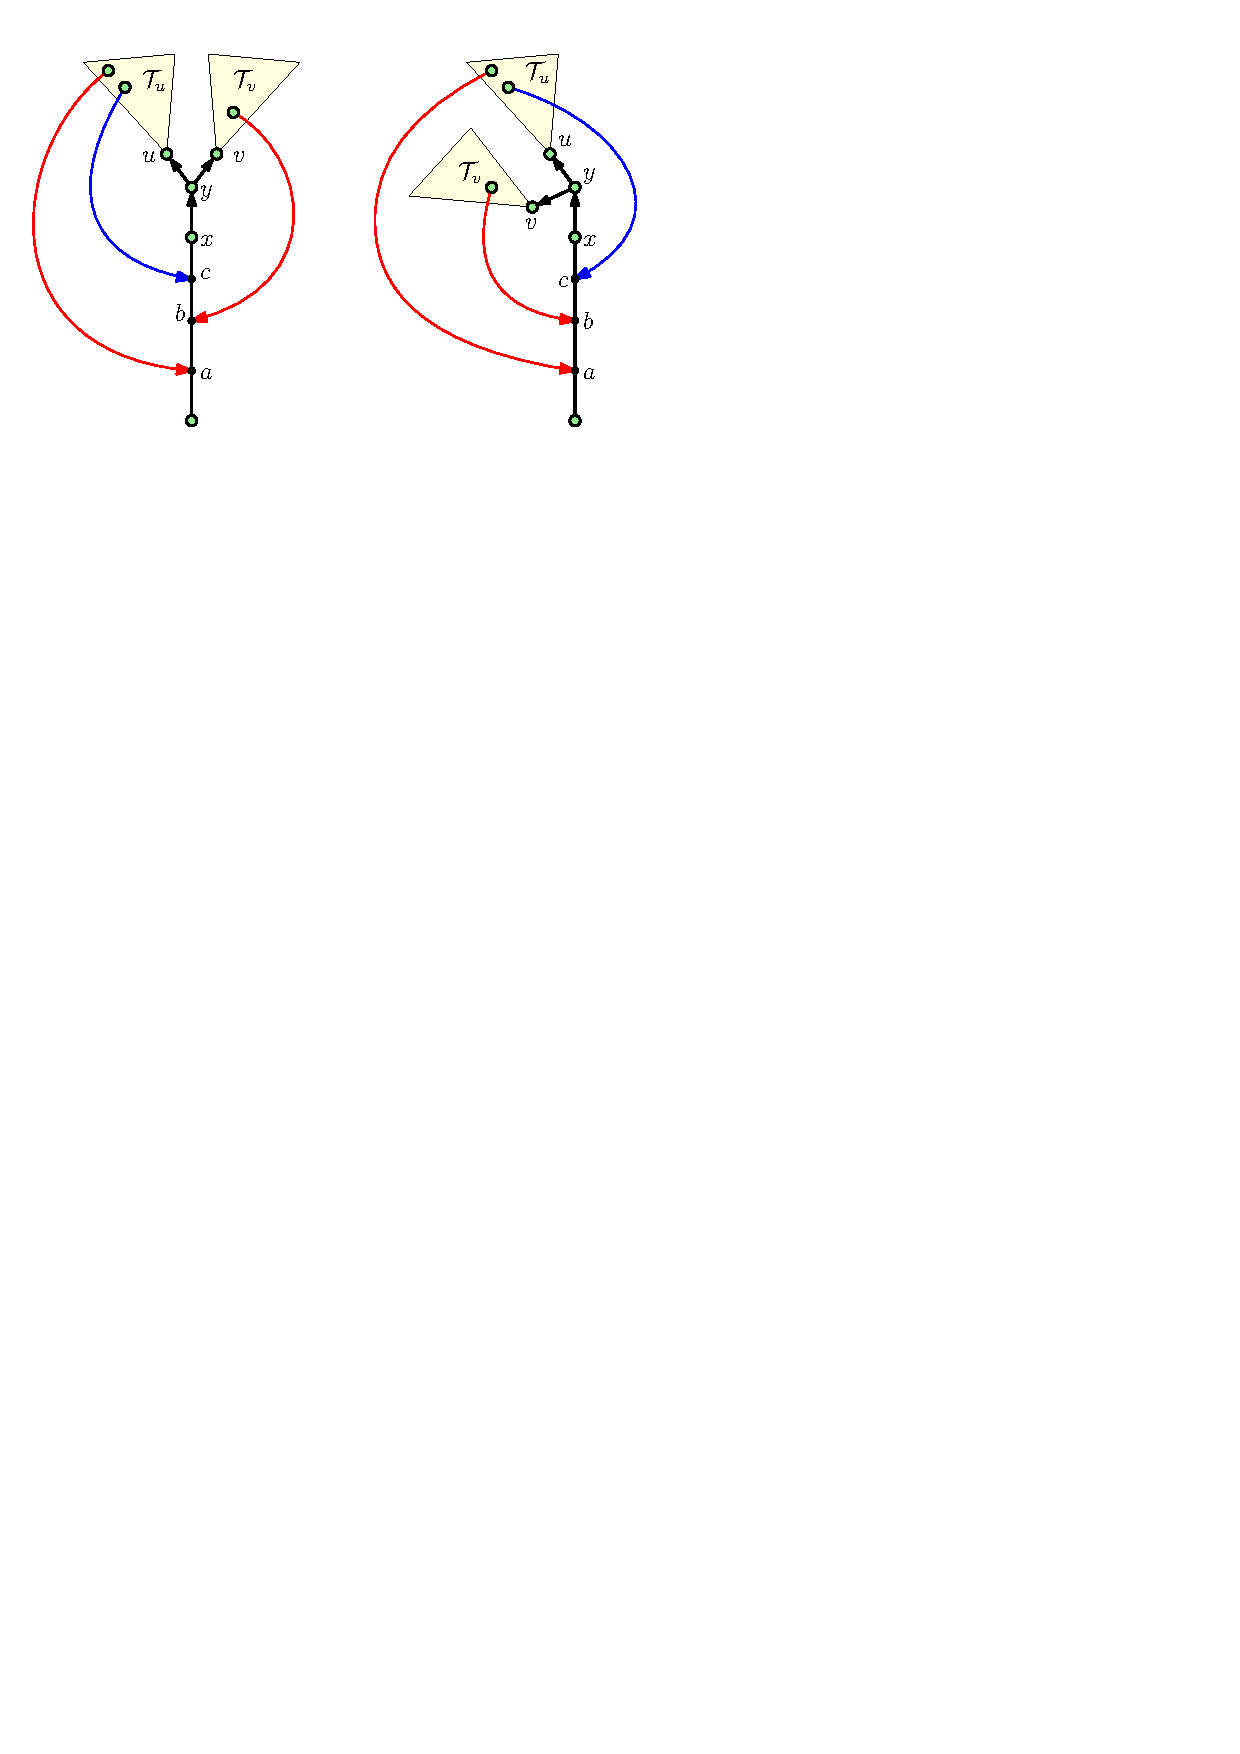
\includegraphics[width=0.32\textwidth]{figures/get_merged_fringe.pdf}\\
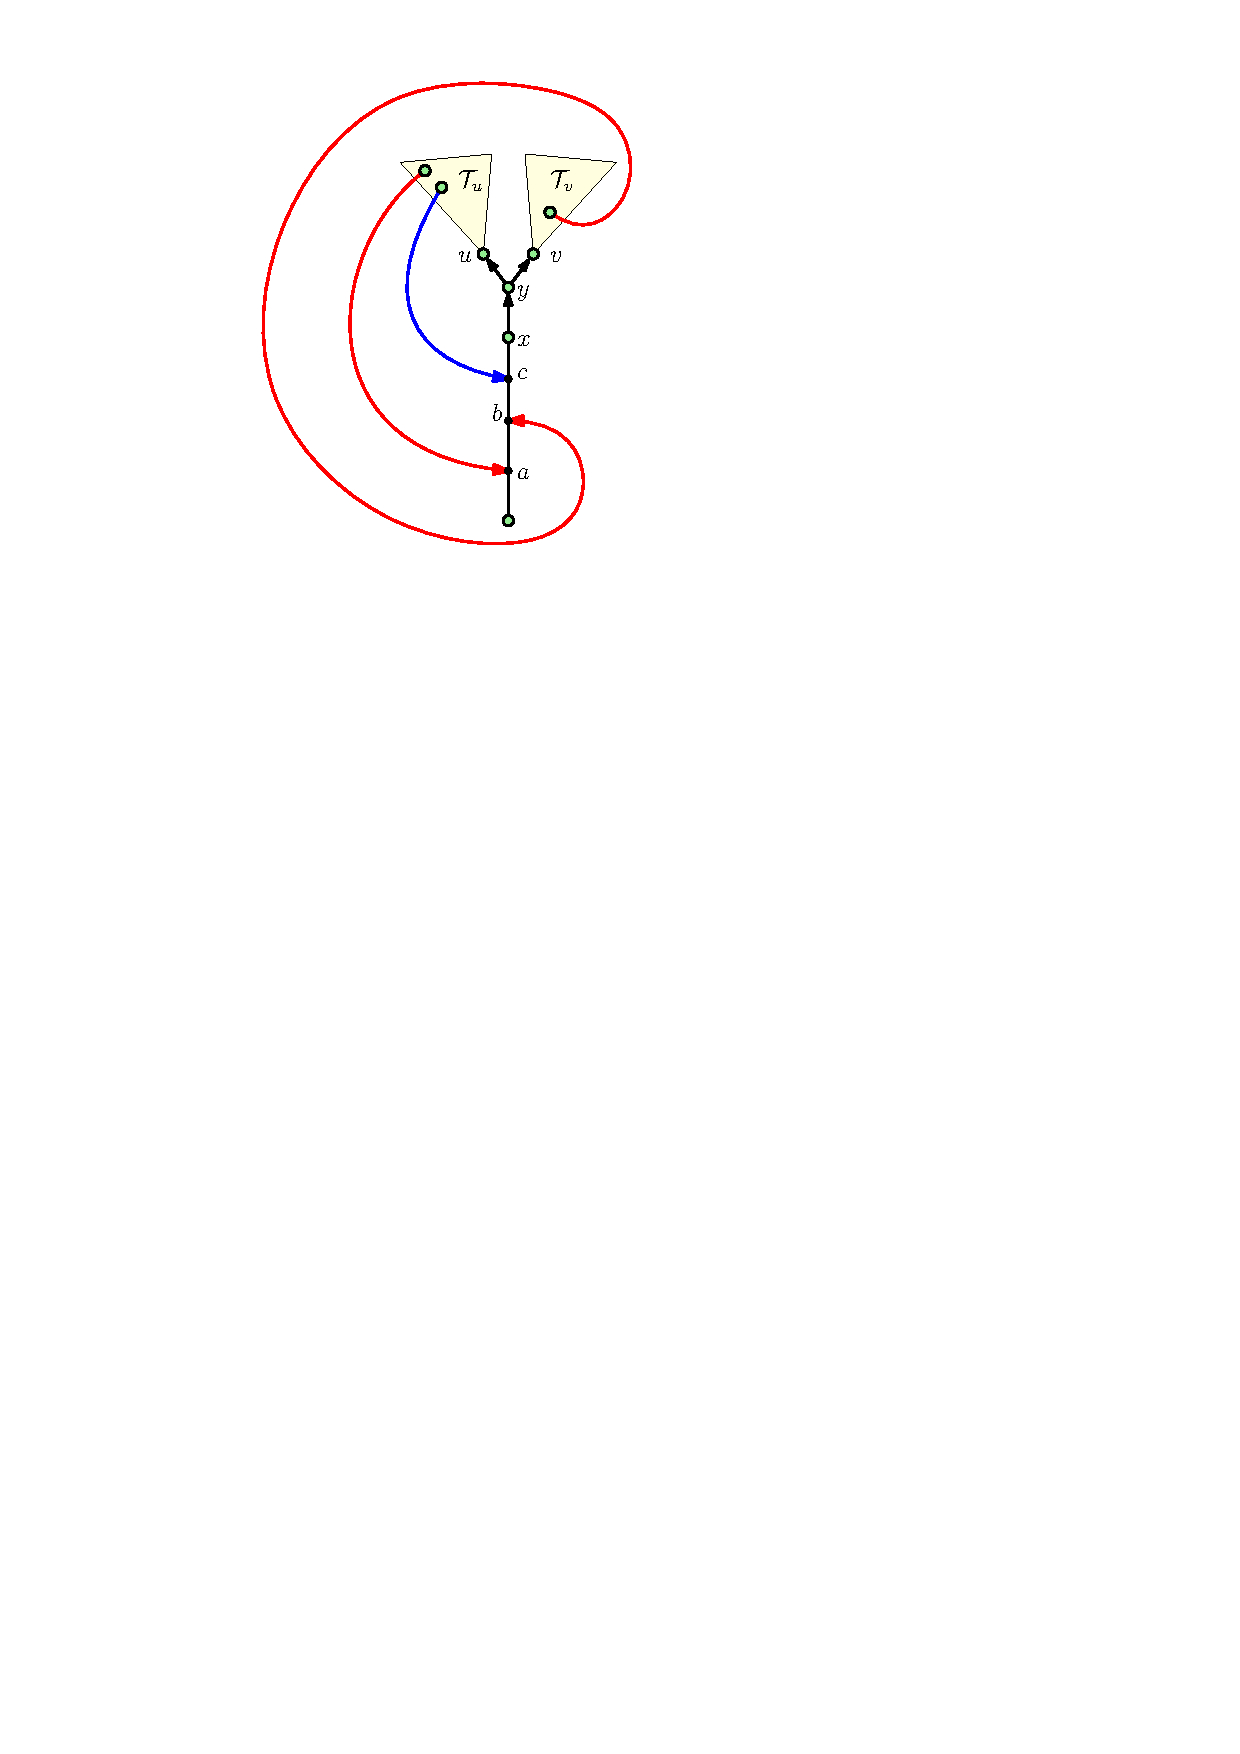
\includegraphics[width=0.16\textwidth]{figures/get_merged_fringe2.pdf}
%\end{figure}
\end{paracol}



\begin{lstlisting}[language=Python, caption=get\_merged\_fringe,escapechar=@,
                   label=lst:get_merged_fringe]
def get_merged_fringe(upper_fringes):
    if len(upper_fringes) > 0:
        upper_fringes.sort()
        new_fringe = upper_fringes[0]
        for f in islice(upper_fringes, 1, len(upper_fringes)):
            new_fringe.merge(f)
        return new_fringe
\end{lstlisting}

\paragraph{整列アルゴリズムについて}
\lstrefname\ref{lst:get_merged_fringe}は
整列アルゴリズムとしてpythonバインドのTimSortを用いているが、
厳密には整数整列アルゴリズムで実装しなければならない。
補木辺の終点の高さは整数なのでビンソートなどを用いれば、
$O(|\omega^+(v)|+|\omega^-(v)|)$時間で処理できる。
各頂点$v$の$\omega^+(v)$および$\omega^-(v)$のサイズの分布を見て
必要に応じて適した整数ソートを実装すると良い。





%%%%%%%%%%%%%%%%%%%%%%%%%%%%%%%%%%%%%%%%%%%%%%%%%%%%%%%%%%%%%%%%%%%%%%%%%%%%%%%%%
\subsection{フリンジの基本的な性質}

フリンジは対象の木辺に関連づく補木辺の集まりであるが、
リストで管理するには簡潔すぎる。
禁止グラフを形成しそうな補木辺の集まりを構造化し、
これをリストする。
禁止グラフを形成しそうな組合せ構造をフリンジ内干渉と呼ぶ。

\subsubsection{フリンジの基本構造}

下記にフリンジクラスのpythonコードの一部を示す。
クラスメソッドなど詳細を含めたコードは節末の\lstrefname\ref{fringe}に示す。
初期化は、空集合もしくは一つの補木辺からなる集合の二通りを受け付け、
クラス{\tt fop}の双方向キュー{\tt self.fops}を作る。

\vspace{-1.\intextsep}
\setcolumnwidth{0.85\textwidth, 0.15\textwidth}
\begin{paracol}{2}
%\begin{lstlisting}[language=Python, caption=クラス fringe,
\begin{lstlisting}[language=Python]
class fringe:
    def __init__(self, dfs_h=None):
        self.fops = deque() if dfs_h is None else deque([fop(dfs_h)])

    @property
    def H(self):
        return self.fops[0]

    @property
    def L(self):
        return self.fops[-1]
\end{lstlisting}

\switchcolumn
\vspace*{2.\intextsep}
\centering

\includegraphics[width=0.11\textwidth]{figures/fringe_basic_code.pdf}
\end{paracol}

フリンジの基本構造は、二つの参照点{\tt L, H}しか持たない簡潔な構造をとる。
{\tt L, H}それぞれ最も根に近い、もしくは遠い終点を持つ補木辺への参照を与える。
フリンジ内のフリンジ内干渉のリストを加工する際、
内側から、すなわち{\tt H}から更新や削除がされる。
{\tt L}はフリンジ内干渉を形成する補木辺の判定で用いられる。







\subsubsection{フリンジ内干渉の定義}

\setcolumnwidth{0.66\textwidth, 0.33\textwidth}
\begin{paracol}{2}
\begin{definition}[フリンジ内干渉]
$v \in V$および$e_1, e_2 \in \omega^+(v)$とする。
$e_1$が橋でないなら、
$e_2$の$e_1$に対するフリンジ内干渉を次のように定義する。
\[
\fop_{e_1}(e_2)=\{(x, y) \in \fringe(e_2) ~:~ y \succ \low(e_1)\}.
\]
$e_1$が橋なら$\fop_{e_1}(e_2) = \varnothing$とする。

また、木辺$e=(x, y)$と補木辺$f=(y, y') \in \omega^-(y)$に対する
フリンジ内干渉も同様に定義する。
$e$が橋でないなら、
\begin{align*}
\fop_e(f) &= \{f ~:~ y' \succ \low(e)\},\\
\fop_f(e) &= \{(x, y) \in \fringe(e) ~:~ y \succ y'\}.
\end{align*}
$e$が橋なら$\fop_e(f)=\varnothing$とする。
\end{definition}




\switchcolumn
\vspace{-1.5\intextsep}
\centering
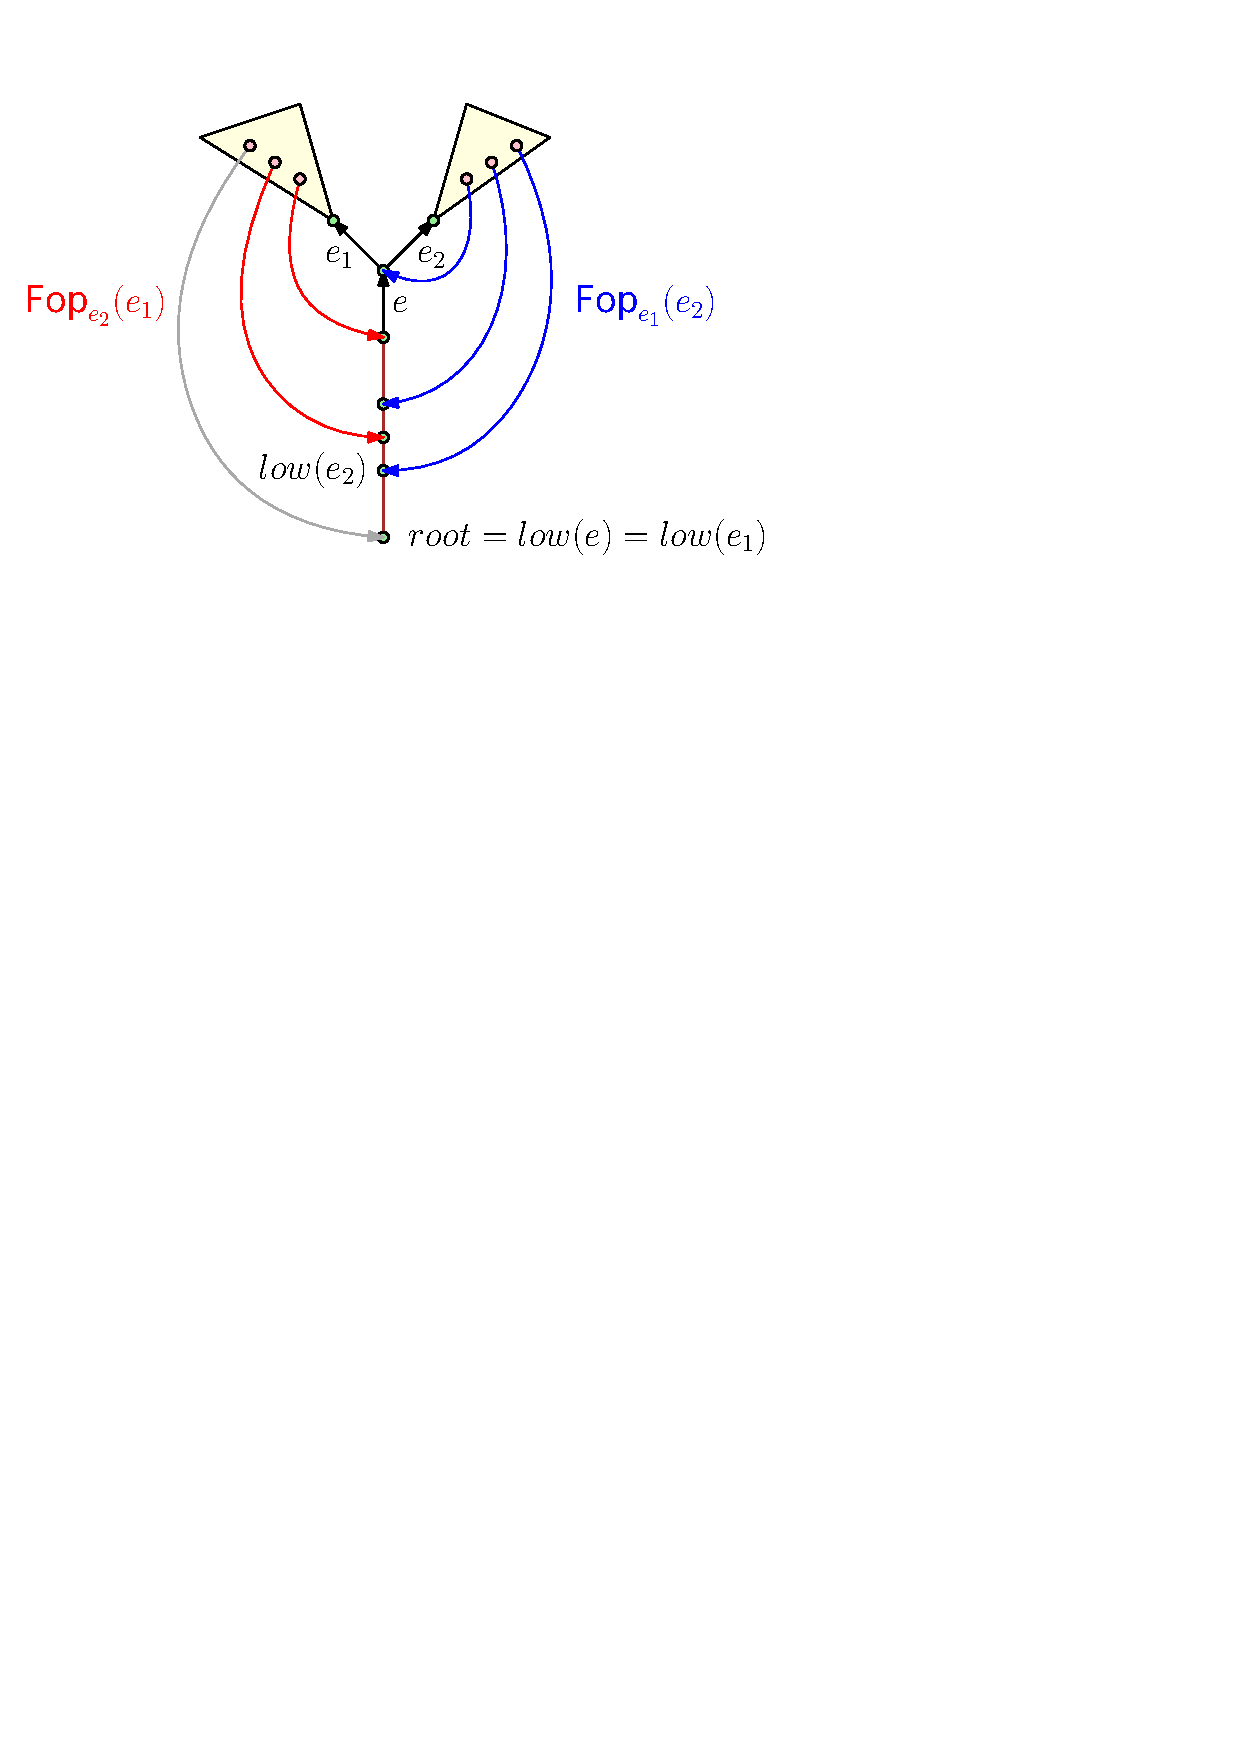
\includegraphics[width=0.3\textwidth]{figures/fop_and_low_1.pdf}

\vspace{0.5\intextsep}
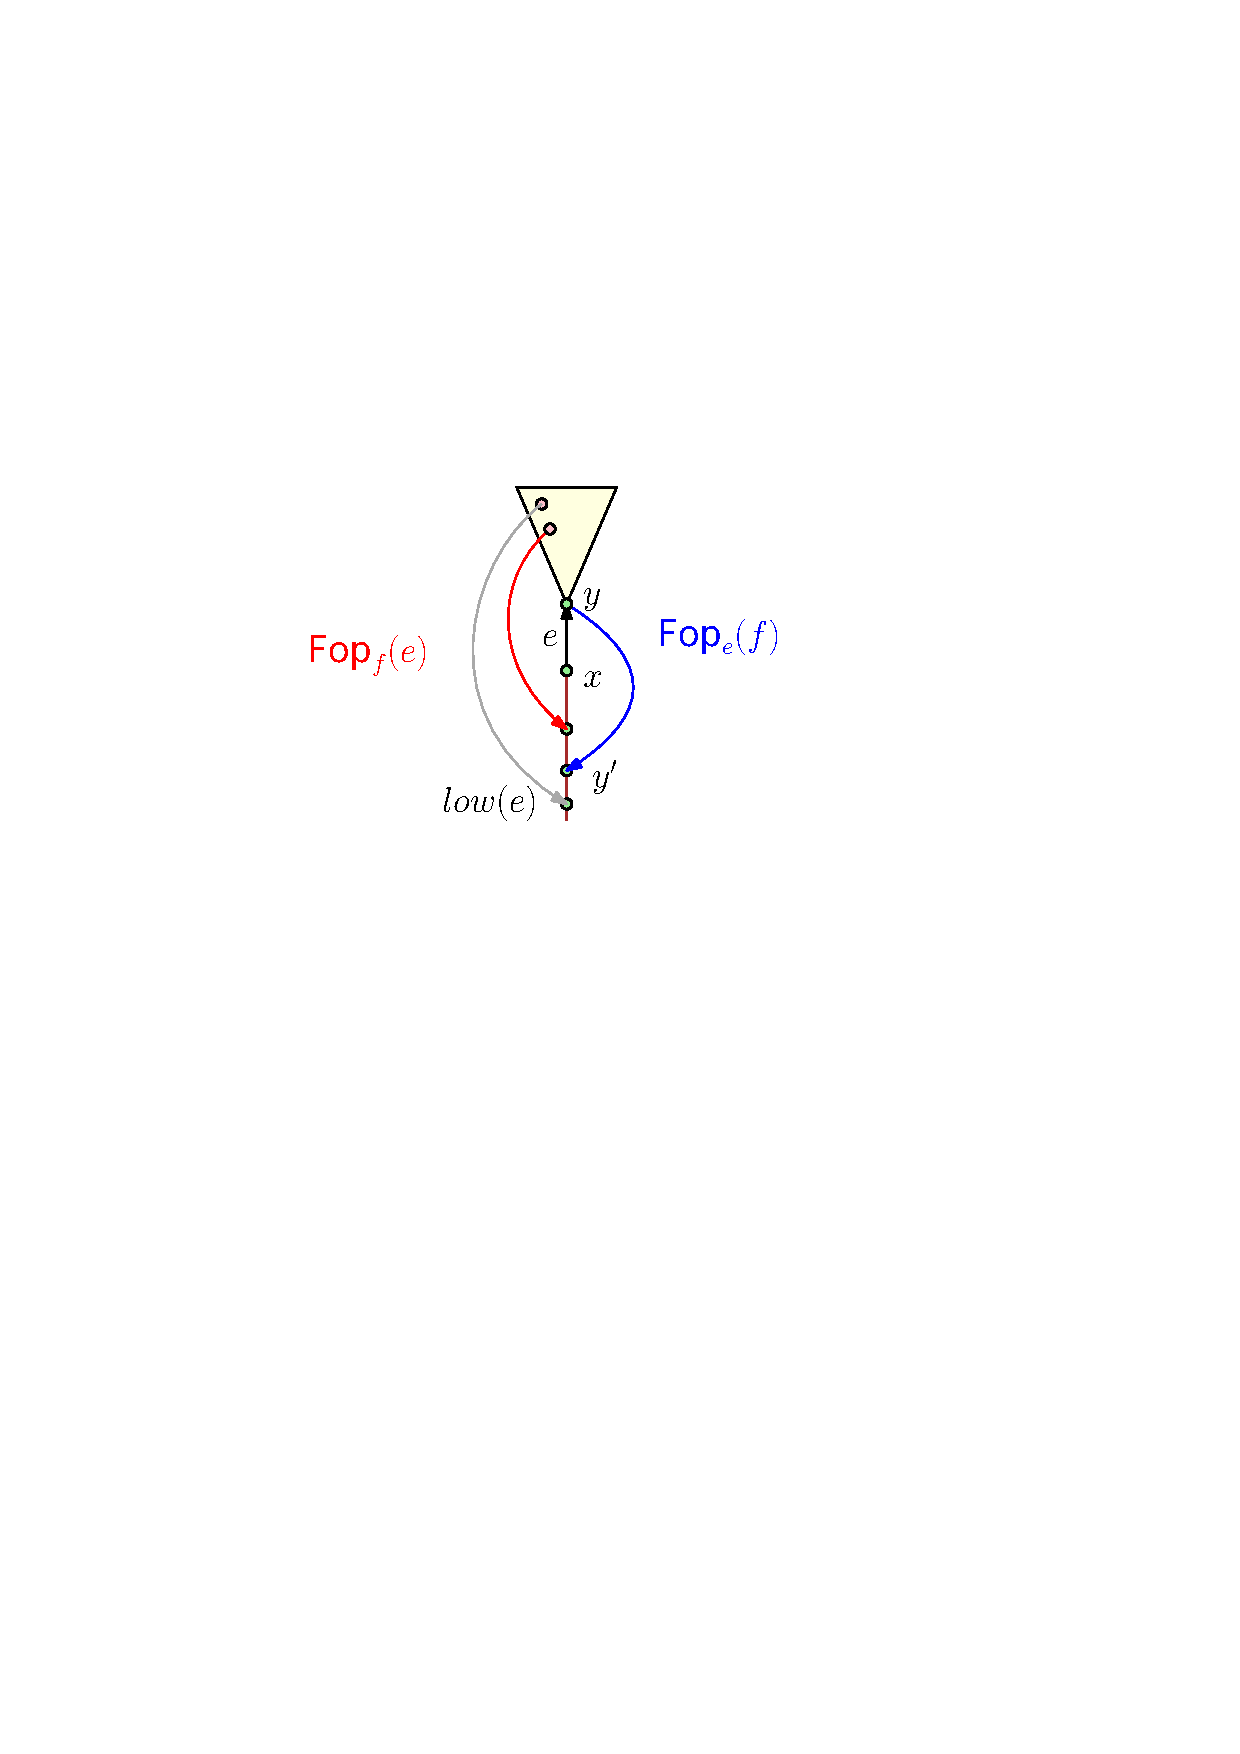
\includegraphics[width=0.22\textwidth]{figures/fop_and_low_2.pdf}
\end{paracol}





\begin{definition}
深さ優先探索木${\mathcal T}=(V, T)$において、
辺集合$T$から頂点集合$V$への写像$\low$を次のように定義する。
\[
\low(e)=\left\{
\begin{array}{ll}
    \argmin_{v\in\tau(e)}\, h(v) ~~~~~~~~ & {\rm if}\ e\ {\rm is\ not\ a\ bridge,} \\
    \bot ~~~~~~~~~~~ & {\rm otherwise.}
\end{array}\right.
\]
ただし、$\tau(e)=\{y ~{\rm for}~ (x, y) \in \fringe(e)\}$とする。
\end{definition}




$\fop_{e_1}(e_2)$と$\fop_{e_2}(e_1)$に属す辺どうし、および
$\fop_e(f)$と$\fop_f(e)$に属す辺どうしは互いに干渉するという。







\subsubsection{フリンジ内干渉のデータ構造}
フリンジ内干渉のデータ構造を\lstrefname\ref{lst:fringe_opposed_subset}に示す。
二つの双方向キューからなる単純な構造だが、
使い方に注意が必要である。
配列{\tt self.c}の二つの双方向キューは、
対象の木辺$(x, y)$に対して${\mathcal T}_y$内の頂点を始点に持ち、
$y$の先祖に終点を持つ%木辺$e_1, e_2$の
互いに干渉する補木辺を管理する。


\setcolumnwidth{0.6\textwidth, 0.4\textwidth}
\begin{paracol}{2}
%\vspace*{-2.\intextsep}
\begin{lstlisting}[language=Python, caption=fringe\_opposed\_subset,escapechar=!,
                   label=lst:fringe_opposed_subset]
class fop:
    def __init__(self, h):
        self.c = [deque([h]), deque()]

    @property
    def left(self):
        return self.c[0]

    @property
    def right(self):
        return self.c[1]

    @property
    def l_lo(self):
        return self.c[0][-1]

    @property
    def l_hi(self):
        return self.c[0][0]

    @property
    def r_lo(self):
        return self.c[1][-1]

    @property
    def r_hi(self):
        return self.c[1][0]
\end{lstlisting}

\switchcolumn
\vspace*{.5\intextsep}

\paragraph{6つの参照点}
ある平面埋込みの木辺$e$のフリンジ内干渉を管理する
データ構造の簡略図を下に示している。
データ構造は6つの参照点を持つ。
左右の双方向キューへの参照{\tt left, right}、
およびそれらの先頭{\tt l\_hi, r\_hi}と末尾{\tt l\_lo, r\_lo}への参照。

\vspace{0.5\intextsep}
%\centering
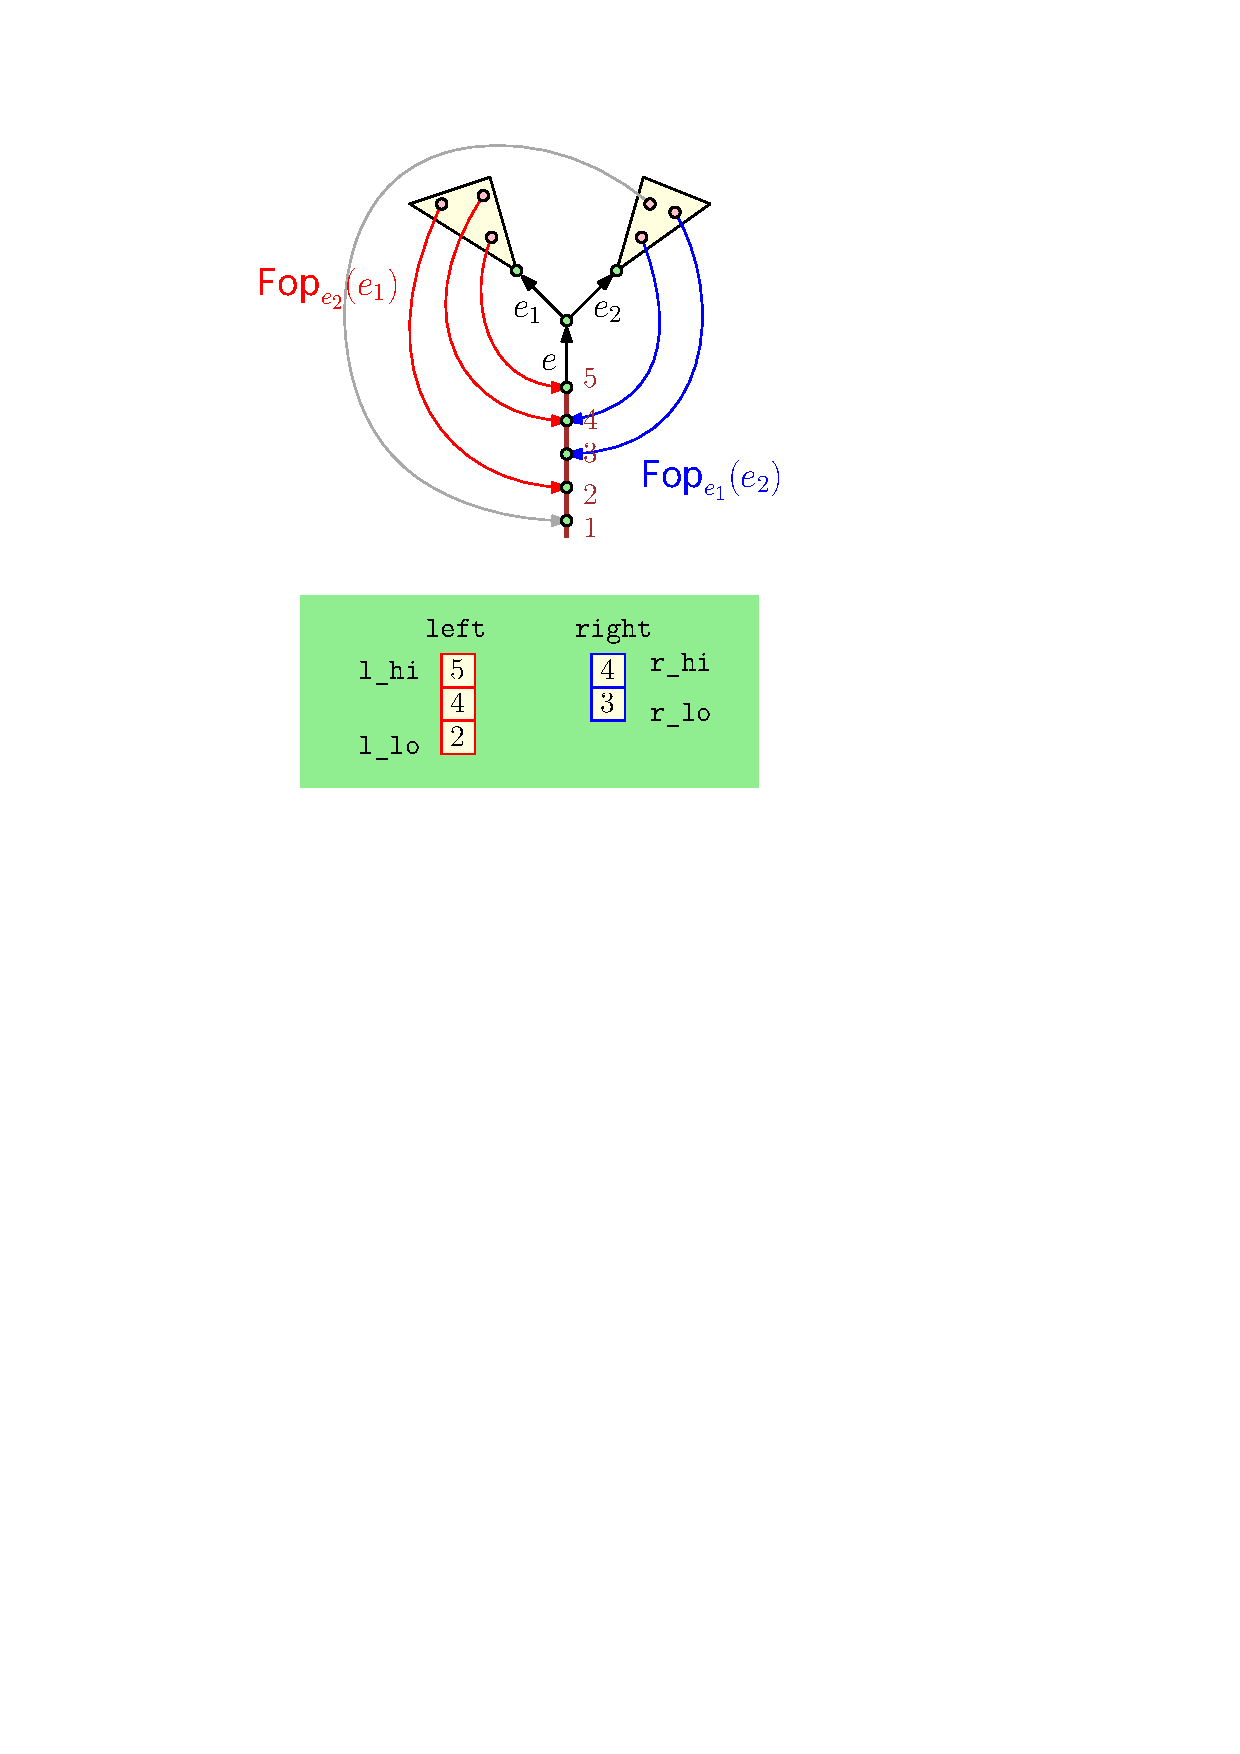
\includegraphics[width=0.27\textwidth]{figures/ds_of_fops.pdf}


\end{paracol}


%%%%%%%%%%%%%%%%%%%%%%%%%%%%%%%%%%%%%%%%%%%%%%%%%%%%%%%%%%%%%%%%%%%%%%%%%%%%%
%\begin{comment}
\paragraph{フリンジ内干渉の文字列表現}
フリンジ内干渉を各補木辺の終点の高さを管理する二つの整数系列の対で表現する。
%この整数は各補木辺の終点の高さを表す。
上図の緑の矩形に囲まれたフリンジ内干渉のデータ構造は%表現 $\varphi$ は
$\varphi=([5,4,2], [4,3])$ のように書ける。
$\varphi$.left.lowで% とアクセスすることで
$\low(e_1)$の高さ$2$を得る。%を取得できる。
%また、上図の灰色の補木辺は別のフリンジ内干渉で定義され$([1], [~])$のように書ける。
%\end{comment}
%%%%%%%%%%%%%%%%%%%%%%%%%%%%%%%%%%%%%%%%%%%%%%%%%%%%%%%%%%%%%%%%%%%%%%%%%%%


\subsubsection{フリンジ内干渉のデータ構造に対する管理規約}
\label{fop_specification}
\paragraph{左優先の管理規約}
各補木辺は可能な限り左側の双方向キューで管理する。
右側の双方向キューは空集合であることが望ましい。
%右が非空である場合は$\varphi$.left.low $< \varphi$.right.low 
%となるようにする。
アルゴリズムの処理過程で左が空集合で右が非空となる場合がある。
その場合、右側の補木辺集合を左に置き換える。
置き換えても問題無いことは\cref{lemma:swap_side}が保証する。


%%%%%%%%%%%%%%%%%%%%%%%%%%%%%%%%%%%%%%%%%%%%%%%%%%%%%%%%%%%%%%%%%%%%%%%
\begin{comment}
\begin{lemma}
フリンジ内干渉の{\tt left}が空で{\tt right}が非空の場合、
{\tt right}の補木辺を{\tt left}に移動させても部分的な平面性は破綻しない。
\end{lemma}

\begin{proof}

\end{proof}
\end{comment}
%%%%%%%%%%%%%%%%%%%%%%%%%%%%%%%%%%%%%%%%%%%%%%%%%%%%%%%%%%%%%%%%%%%%%





\paragraph{補木辺の位相不変性}
平面性判定の処理過程において、フリンジ併合および補木辺除去によって
各双方向キュー内の終点の高さに関する非増加順序を乱さないことを保証しなければならない。
この不変性により、補木辺どうしの干渉性、
あるフリンジを別のフリンジの入れ子にできるかどうか、
不要になった補木辺の除去などの手続きが
定数時間で処理できることを保証できる。
このフリンジ内干渉の位相不変性は、
アルゴリズムの線形時間計算量を保証する上で最重要事項である。






\paragraph{フリンジ内干渉の取り扱い}
管理規約に従うと干渉し合う補木辺の入れ替えは、
具体的に\lstrefname\ref{lst:t_opposite}のように
{\tt fringe}のクラスメソッド{\tt \_merge\_t\_opposite\_edges\_into}として記述できる。
双方向キュー{\tt left}は{\tt right}の末尾に連結されるので$O(1)$時間で完了する。
従って計算量は、
第2行のループ回数$O(|\omega^+(v)| + |\omega^-(v)|)$で抑えられる。


%{\tt left}の補木辺は一度{\tt right}に
%移されたら戻ることはないので$O(|\omega^+(v)|+|\omega^-(v)|)$時間で完了する。
\setcolumnwidth{0.75\textwidth, 0.25\textwidth}
\begin{paracol}{2}
%\vspace{-2.\intextsep}
\begin{lstlisting}[language=Python, caption=\_merge\_t\_opposite\_edges\_into,
                   label=lst:t_opposite]
    def _merge_t_opposite_edges_into(self, other):
        while (not self.H.right and self.H.l_hi > other.H.l_lo):
            other.H.right.extend(self.H.left)
            self.fops.popleft()
\end{lstlisting}

\switchcolumn
\vspace{0.5\intextsep}
\centering
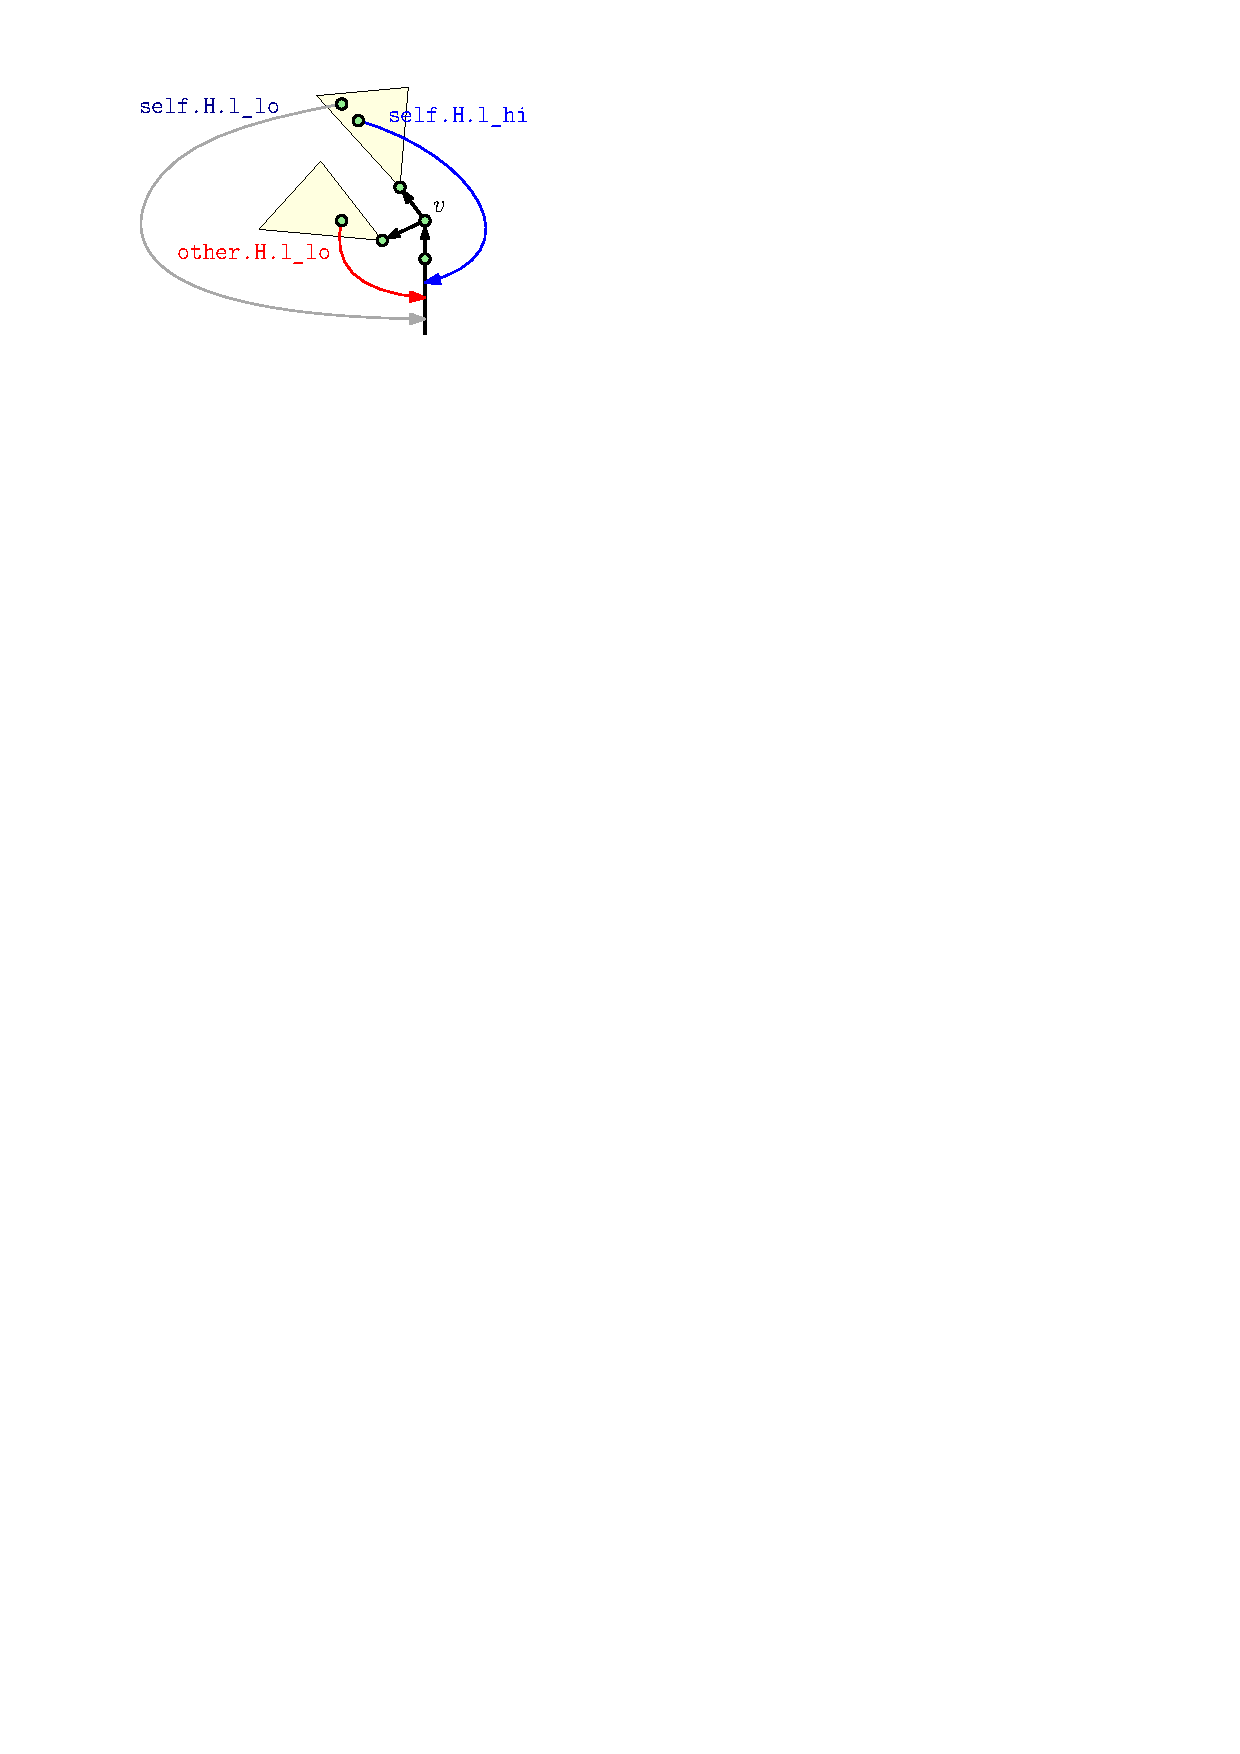
\includegraphics[width=0.24\textwidth]{figures/t_opposite.pdf}
\end{paracol}












%%%%%%%%%%%%%%%%%%%%%%%%%%%%%%%%%%%%%%%%%%%%%%%%%%%%%%%%%%%%%%%%%%%%%%%%%%%%%%%%%%%%%%%%%
\subsubsection{フリンジ内干渉を利用したクラトフスキー部分グラフの検出}

フリンジ内干渉の{\tt right}が非空の場合、その初等閉路の集まりが誘導する部分グラフが
極大な非クラストフキーグラフを形成することを確認する。
つまり
{\tt right}が非空の状態で内から外へ接続する補木辺が存在するとき、
直ちに非平面的と判定できることを示す。
%ここでは、具体的な検出手続きを記述し、その計算量と正当性を考察する。





\setcolumnwidth{0.66\textwidth, 0.33\textwidth}
\begin{paracol}{2}
\paragraph{子孫フリンジの縮約}
最初の例は、
フリンジ内干渉の{\tt left}サイドに補木辺の集まりを仮想的に縮約する手続きである。
具体的な pythonコードを\lstrefname\ref{lst:_merge_t_alike_edges}に示す。
まずは状況確認から。
木辺$e=(x,y)$のフリンジ$\fringe(e)$を形成しようとしている。
このとき子孫の木辺$e_i \in \omega^+(y)$の各フリンジは形成済みであり、
それぞれクラトフスキーグラフを含まない、つまり平面的とする。
また、$k=|\omega^+(y)|$とし、
$e_1, \ldots, e_k$は$h(\low(e_i))$に関して昇順に採番されている。
縮約対象は各木辺$e_2, \ldots, e_k$の各フリンジ内干渉のリスト{\tt fops}である。


\switchcolumn
\vspace{.5\intextsep}
\centering
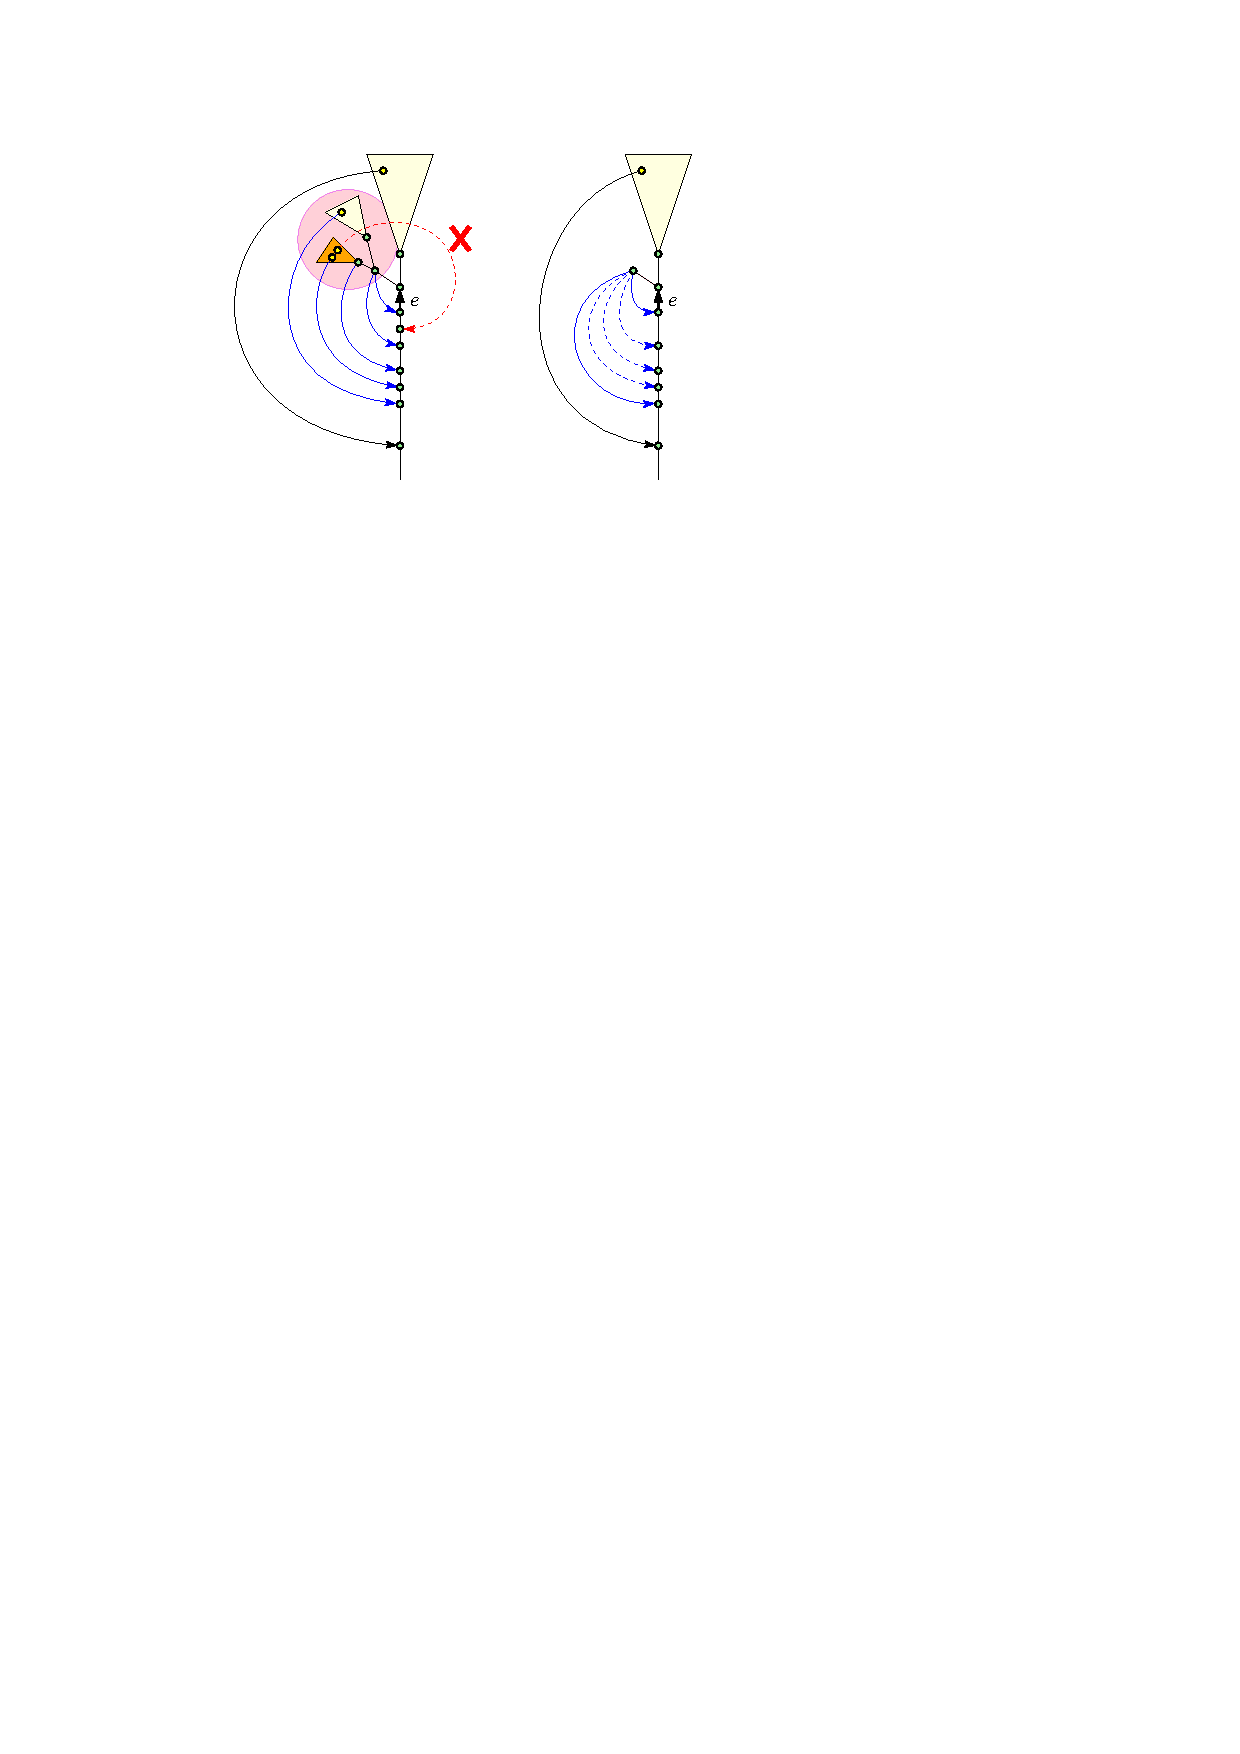
\includegraphics[width=0.31\textwidth]{figures/merge_t_alike_edges.pdf}

\end{paracol}


右図左の丸で囲まれたフリンジを縮約対象とし考察する。右が所望の縮約結果である。
すべての補木辺が{\tt left}サイドに配置されているならクラフトスキーグラフは存在しない。
$\low(e_1)$を終点とする補木辺が存在するので、
いずれの補木辺も部分的に{\tt right}に配置することはできない。
{\tt right}に配置する場合は全ての補木辺を{\tt fops}内の順序を変えること無く
移動させなければならない。
以上のことから
仮想的な頂点を始点とするよう縮約して扱う必要がある。



\begin{lstlisting}[language=Python, caption=\_merge\_t\_alike\_edges,escapechar=@,
                   label=lst:_merge_t_alike_edges]
    def _merge_t_alike_edges(self):
        if self.H.right:
            raise Exception
        for f in islice(self.fops, 1, len(self.fops)):
            if f.right:
                raise Exception
            self.H.left.extend(f.left)
        self.fops = deque([self.fops[0]])
\end{lstlisting}



このときオレンジの部分木のように、
{\tt left, right}両サイドに補木辺が配置されるフリンジ内干渉が存在する場合
クラフトスキーグラフを形成する。
第2行および第5行のように{\tt if self.H.right}で非空を判定し、
真のとき例外{\tt Exception}を生成し平面的でないと判定し処理を完了する。
そうでない場合は第7行のように、
先頭のフリンジ内干渉の双方向キュー{\tt left}の末尾に連結する。
最終的に第8行のように唯一のフリンジ内干渉に縮約されるので、
参照点{\tt H}の利用はそれほど本質的ではない。

\paragraph{計算量と正当性}
\lstrefname\ref{lst:_merge_t_alike_edges}の
第4行の{\tt for}ループの内部は1つの条件式と連結リストの結合なので$O(1)$。
ループ回数はフリンジ内干渉のリスト{\tt fops}のサイズなので
$O(|\omega^+(v)|+|\omega^-(v)|)$で抑えられる。
正当性は\cref{lemma:t_alike}に従う。

\begin{lemma}
\label{lemma:t_alike}
\lstrefname\ref{lst:_merge_t_alike_edges}が例外を生成するなら
クラトフスキー部分グラフが存在する。
\end{lemma}



\setcolumnwidth{0.66\textwidth, 0.33\textwidth}
\begin{paracol}{2}
\begin{proof}
{\tt right}が非空になる二通りの場合を考察する。

まず、フリンジ内干渉を形成するには、右図左下段のように五つの頂点の下で、
三つの補木辺(シアン)と四つの木辺(黒)が少なくとも必要である。
%五頂点のうち補木辺の始点と終点の組合せは右図のように上$2$下$3$以外に
%上$3$下$2$も考えられる。
補木辺の始点の中で最も根に近い頂点を$v$、終点の中で最も根から離れている頂点を$x$とする。
\lstrefname\ref{lst:_merge_t_alike_edges}が呼ばれる状況、つまり
${\mathcal T}_v$の頂点を始点とする補木辺を継承して
フリンジを形成することを考える。
%このとき\cref{lemma:ignoring_back_edges}は、
%$v$を始点とする補木辺か
%$x$を終点とする補木辺%のいずれか
%を対象外とするので、
このとき、木辺$(x, v)$を細分するような頂点$y$が存在し、
$y$を始点とし高さが$h(\low((y, v)))$以下の頂点を終点とする別の
補木辺も存在するとする(右図赤辺)。
頂点と辺の個数$n,~m$を見積もるとそれぞれ$n=6, m=9$を得る。
この部分グラフの内周$\gamma$は$4$なので
\cref{coro:girth}より
平面的グラフなら
$m \leq \frac{\gamma}{\gamma-2}(n-2)$を満たさなければならないが
$9\leq 8$となる。
これは$K_{3,3}$の細分を形成することを意味する。

別の{\tt right}が非空の場合を考察する。
右図の$\omega^-(v)$と$\omega^-(w)$は互いに干渉するので、
{\tt right}が非空のフリンジ内干渉を形成する。
いま木辺$(x, y)$のフリンジを形成しようとしている。
先ほど同様$y$を始点とし高さが$h(\low((y, v)))$以下の頂点を終点とする別の
補木辺も存在するとする(右図赤辺)。
このとき右図右のように黒辺が存在しなければ平面埋込みは存在するが、
黒辺が存在するので平面性は成り立たない。
$\{r, x, y, v, w\}$が導出する部分グラフは$5$-頂点で$4$-正則なので
$K_5$を形成する。

いずれの場合もクラトフスキー部分グラフを形成する。
\end{proof}

%木辺の系列内の中央三つ目の頂点がフリンジを形成しようとしている木辺$(x, y)$の終点$y$にあたる。
%木辺の個数は\cref{coro:ignoring_back_edges}から、
%3つの補木辺は異なる二つの始点と異なる三つの終点が必要な事実に則る。


%根に近い方から三つ目の木辺を細分して分断に使った頂点を$y$、
%$y$の根に近い方の隣接頂点を$x$とする。
%これは\cref{coro:ignoring_back_edges}から、
%$x$の子孫に補木辺の始点となる三つ必要であり、
%同様に$y$の先祖にも任意の補木辺の終点となる三つの異なる頂点が存在しなければならない
%事実に基づく。

%また、アルゴリズムの入力条件として$\low(y)$を終点として持つ補木辺を含む
%別のフリンジが存在する。
%このとき木辺$e=(x, y)$のフリンジを形成することを考える。
%$e_1$として$y$と$\low(e)$を接続する辺が存在する。
%ここまでで頂点は少なくとも$6$、木辺は$5$、補木辺は$4$存在する。

%従って、
%上記$4$つの初等閉路が誘導する部分グラフはクラトフスキー部分グラフを形成する。


\switchcolumn
\vspace{2.\intextsep}
%\centering
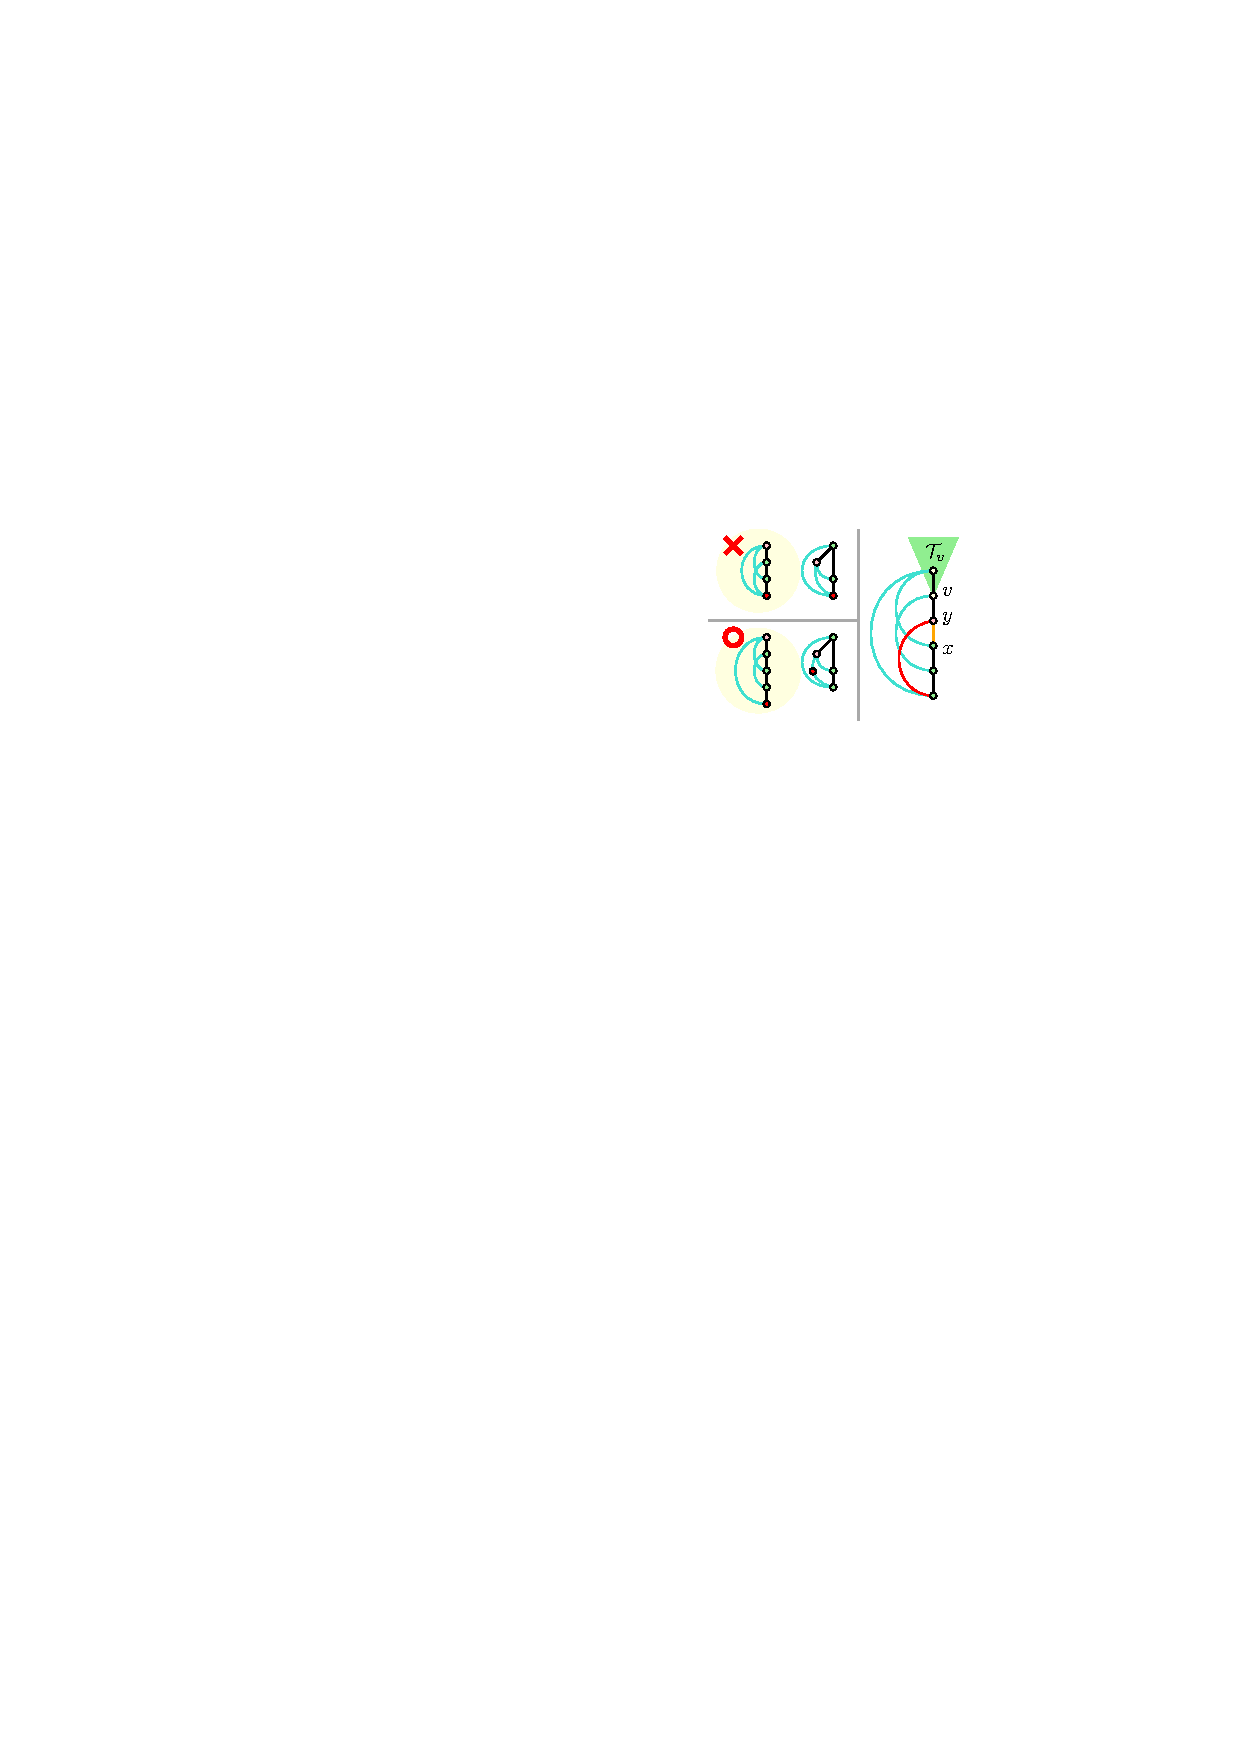
\includegraphics[width=0.29\textwidth]{figures/forbidden_fringe2.pdf}\\
%{\small 左下段は、いずれかの補木辺の内部に根を埋め込まなければならず、
%根は外面に属すという前提に反する。
%従って、内側の補木辺のどちらかは{\tt right}に配置される。}\\
\vspace{0.5\intextsep}
\centering
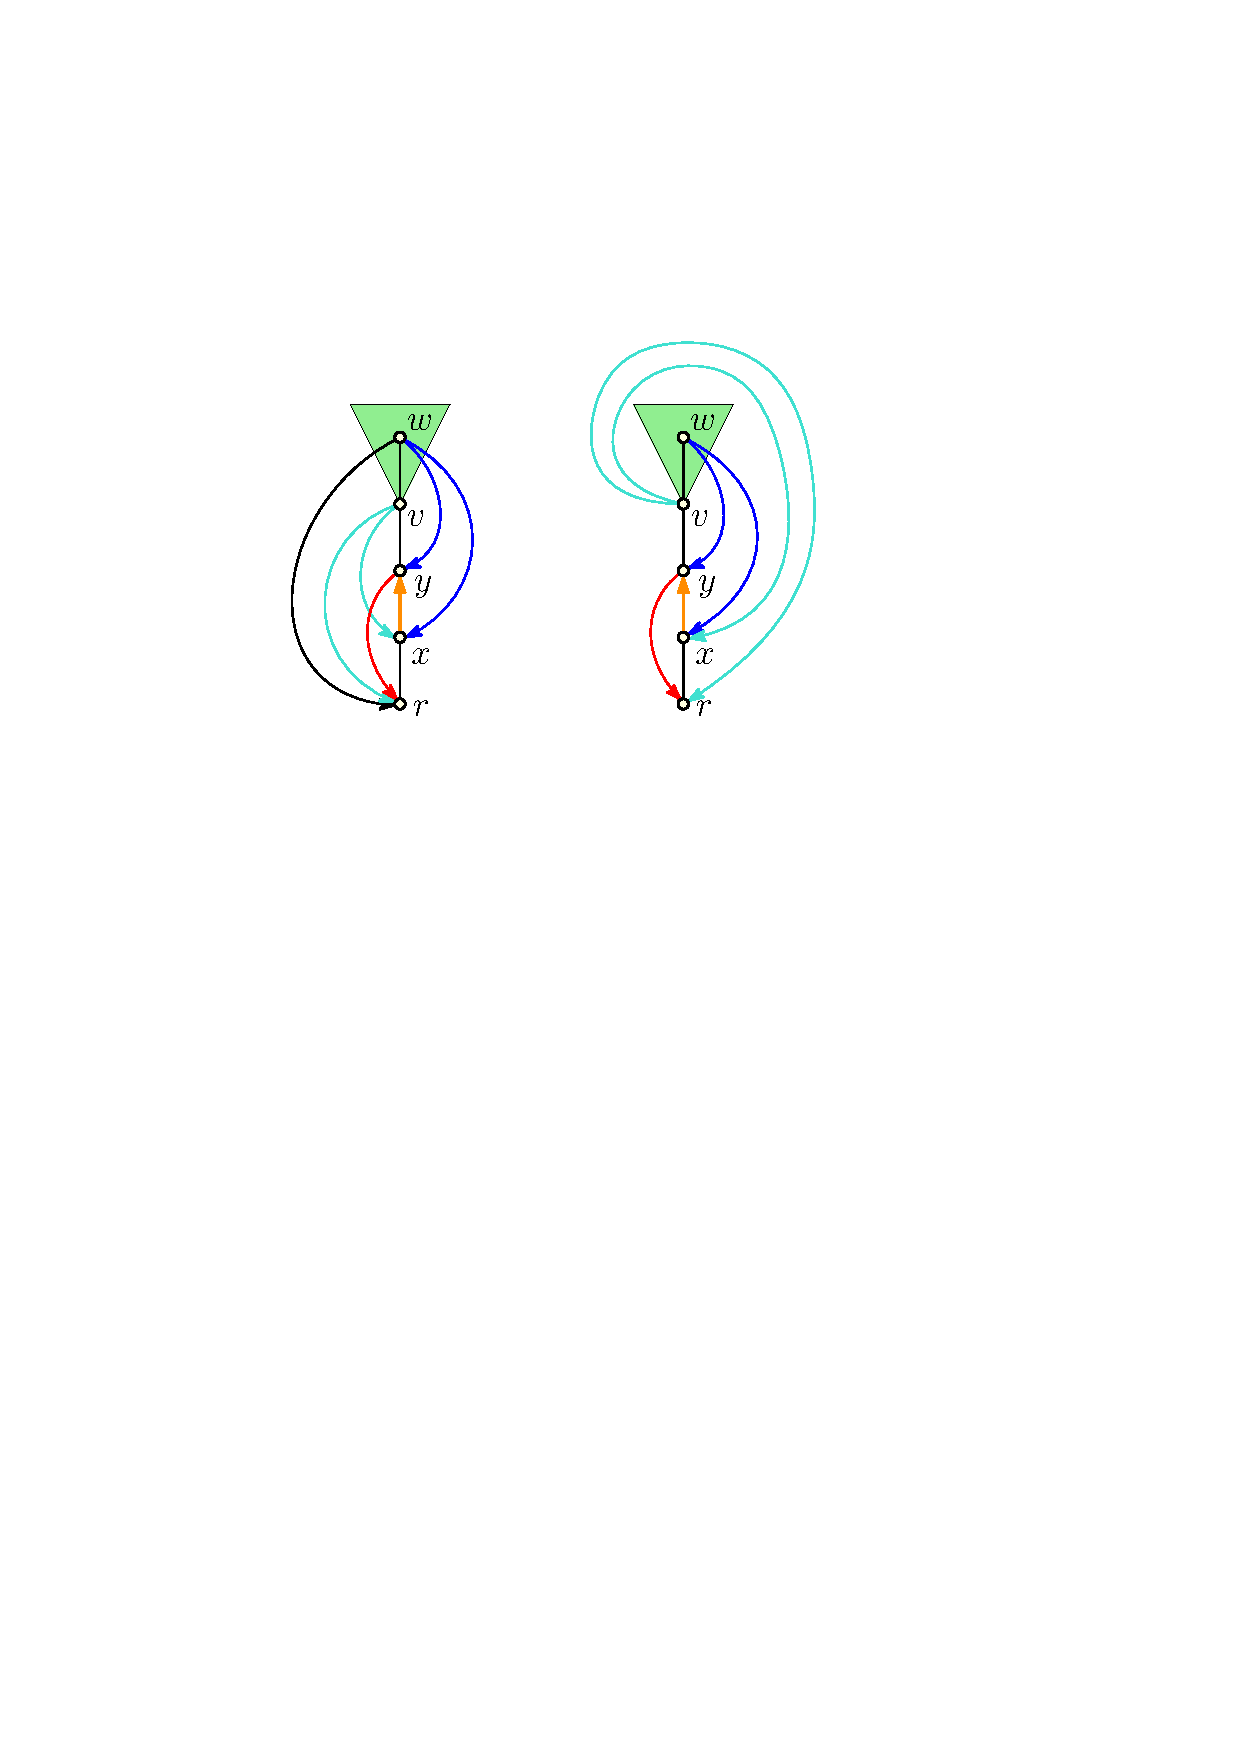
\includegraphics[width=0.32\textwidth]{figures/proof_onions.pdf}
%\vspace{.5\intextsep}
%\hspace{-1.8em}
%{\small 内周はグラフの最小閉路のサイズであり、閉路が存在しない場合は$\infty$をとる。}
\end{paracol}






\setcolumnwidth{0.6\textwidth, 0.4\textwidth}
\begin{paracol}{2}
\paragraph{正しい玉ねぎ構造の埋込み}
次の禁止グラフの検出は、
対象木辺$e=(x, y)$に対する
$e_1, e_2 \in \omega^+(y)$のフリンジの併合に関する手続きである。
$h(\low(e_1)) \leq h(\low(e_2))$とする。
また$\fringe(e_1)$は{\tt right}が
非空のフリンジ内干渉$\gamma_1=([h(u_2), h(u_1)], [h(u_3)])$を持つ。
ただし、$h(u_1) < h(u_2)$かつ$h(u_1) \leq h(u_3) \leq h(u_2)$。
同様に$\fringe(e_2)$は{\tt right}が空だが$\gamma_1$と干渉する
$\gamma_2=([h(v)], [~])$を持つ。
$\gamma_1$と$\gamma_2$が干渉する場合$h(u_3)$と同様に
$h(u_1) \leq h(v) \leq h(u_2)$を満たす。
このとき$h(v) < h(u_3)$ならクラトフスキー部分グラフを形成する(右図右)。

\switchcolumn
\vspace{1.5\intextsep}
\centering
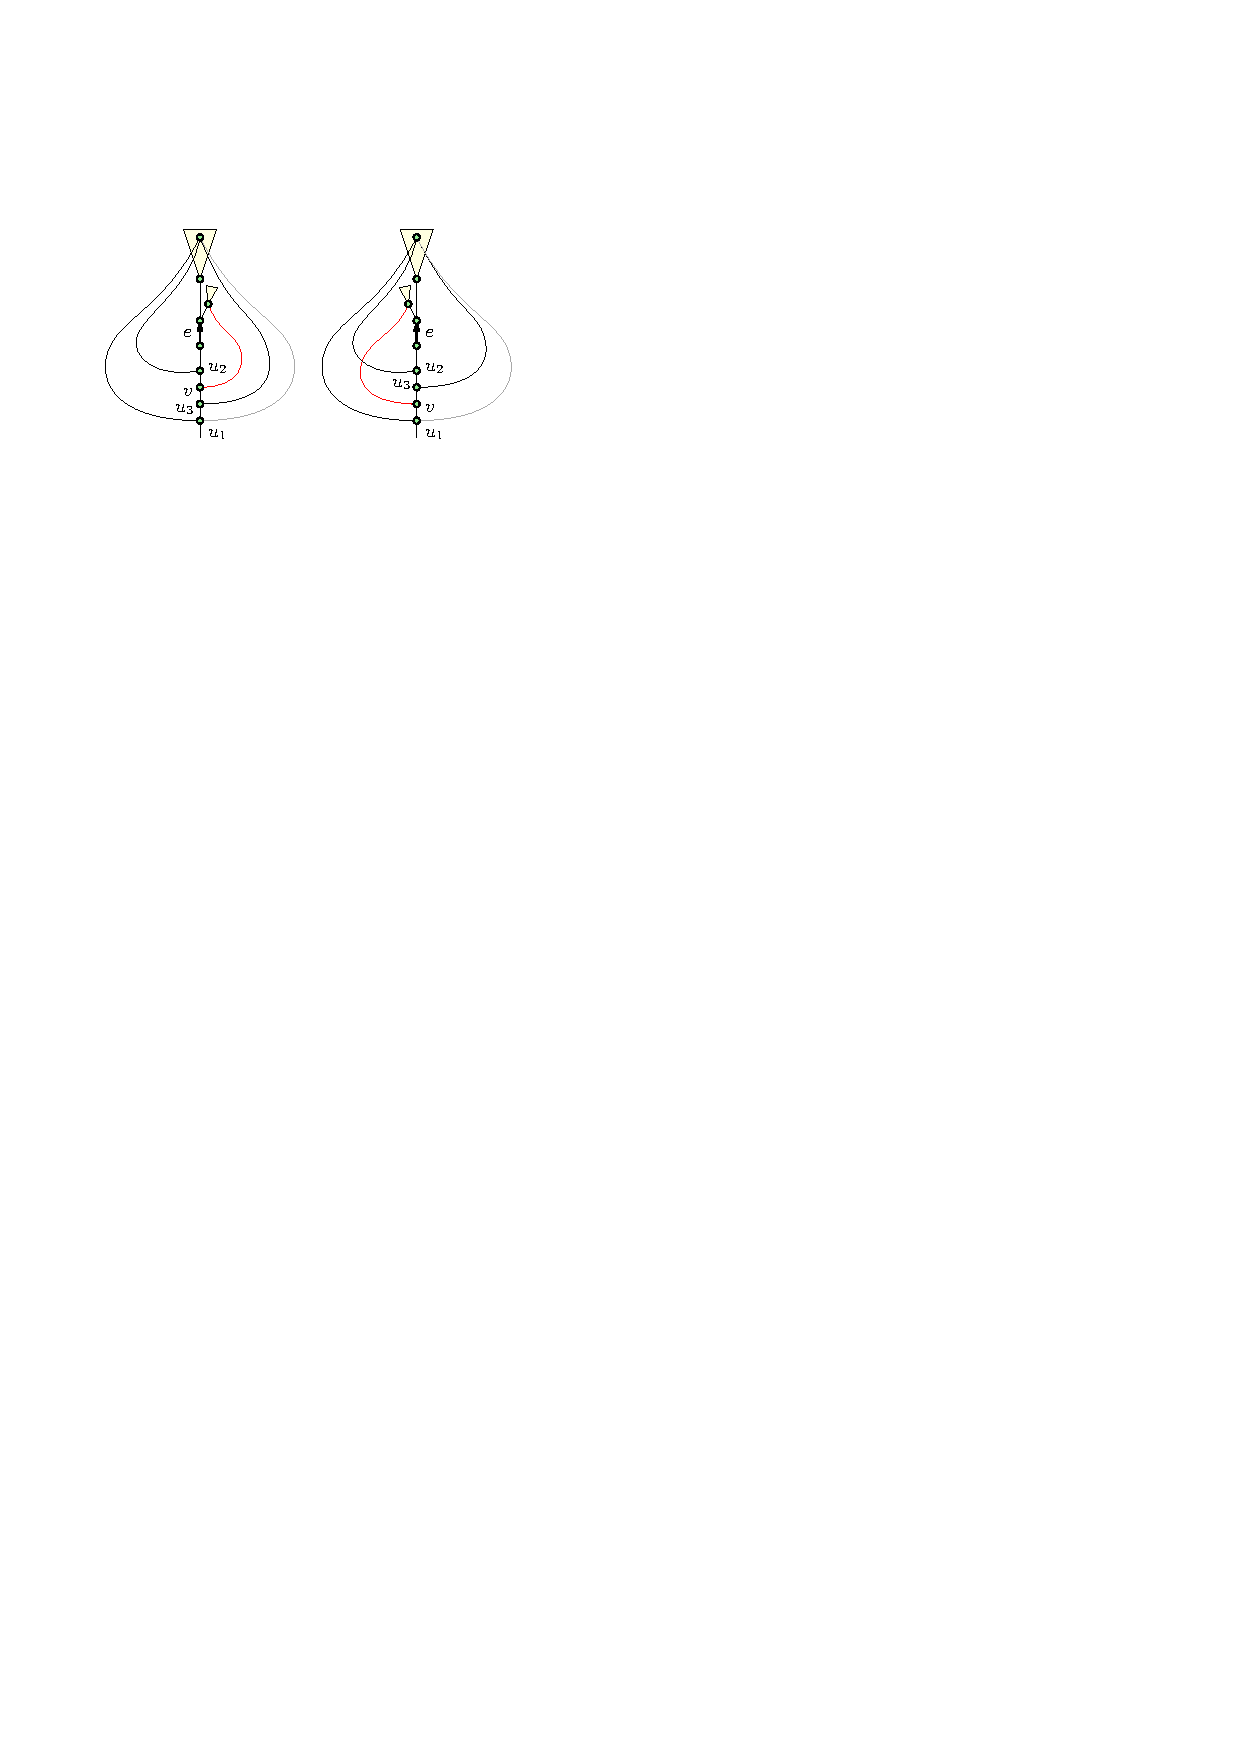
\includegraphics[width=0.37\textwidth]{figures/make_onion.pdf}
\end{paracol}

具体的なpythonコードの例を\lstrefname\ref{lst:_make_onion_structure}に示す。
{\tt self}が$\fringe(e_1)$で{\tt other}が$\fringe(e_2)$。
このとき{\tt self}の
最も根から離れている終点の高さ{\tt self.H.l\_hi}および{\tt self.H.r\_hi}を見て
いずれかの内部に{\tt other}のフリンジ内干渉を埋め込めるかを確認する(第2・3行)。
埋め込めるようであれば{\tt self}の双方向キューに{\tt other}の要素を連結する(第6-9行)。
それ以外の場合は非平面的なので処理を完了する(第4行)。





\setcolumnwidth{0.72\textwidth, 0.28\textwidth}
\begin{paracol}{2}
\begin{lstlisting}[language=Python, caption=\_make\_onion\_structure,
                   label=lst:_make_onion_structure]
    def _make_onion_structure(self, other):
        lo, hi = (0, 1) if self.H.l_hi < self.H.r_hi else (1, 0)
        if other.H.l_lo < self.H.c[lo][0]:
            raise Exception
        elif other.H.l_lo < self.H.c[hi][0]:
            self.H.c[lo].extendleft(reversed(other.H.left))
            self.H.c[hi].extendleft(reversed(other.H.right))
            other.H.left.clear()
            other.H.right.clear()
\end{lstlisting}


\switchcolumn
\vspace{1.\intextsep}
\centering
\includegraphics[width=0.27\textwidth]{figures/illegal_onion_conditions.pdf}
\end{paracol}

玉ねぎ構造という名称は別にふざけて呼んでいるわけではない。
幾何学的グラフに準ずる組合せ構造の列挙や数え上げに対して
用いられる層構造を呼称する際に用いられている。
また、平面的グラフを対象とする最適化問題の多くは、
ベイカーのやり方に代表される層構造を利用したアプローチが広く用いられる。

\paragraph{計算量と正当性}
\lstrefname\ref{lst:_make_onion_structure}は
三つの条件式および連結リストの結合と破棄なので$O(1)$で完了する。
pythonの{\tt collections.deque.extendleft}は最悪の場合
$O(|\omega^+(v)|+|\omega^-(v)|)$時間かかるので
必要に応じて実装を見直す必要がある。
ただ、ここで結合された要素は以降のフリンジ形成において削除されるまで
入れ替えられることはないので全体の計算量へは漸近的に影響しない。
また、正当性は\cref{lemma:onion}に従う。

%\setcolumnwidth{0.85\textwidth, 0.15\textwidth}
%\begin{paracol}{2}
\begin{lemma}
\label{lemma:onion}
\lstrefname\ref{lst:_make_onion_structure}が例外を生成するなら
クラトフスキー部分グラフが存在する。
\end{lemma}


\begin{proof}
\cref{lemma:t_alike}の証明と同様の議論が成り立つ。
\cref{lemma:t_alike}では、
{\tt right}が空のフリンジ内干渉に対して
{\tt right}が非空のフリンジ内干渉を併合する手続きだが、
ここではその逆の場合なので結局クラトフスキー部分グラフを持つ。
%
%
%とりうる場合は二通りある。
%前者は、\cref{lemma:t_alike}において
%シアンの補木辺の集まりを{\tt self}、赤の補木辺を{\tt other}と見立てる逆の構成であり、
%後者は右図に示す
%緑の部分木${\mathcal T}_v$の補木辺の集まりを{\tt self}、
%赤辺を{\tt other}とする構成である。
%前者は$K_{3,3}$の細分となり、
%後者は$5$-頂点$4$-正則なグラフなので$K_5$の細分となる。
\end{proof}

%\switchcolumn
%\vspace{0.5\intextsep}
%\centering
%\includegraphics[width=0.1\textwidth]{proof_onions.pdf}
%\end{paracol}




\subsubsection{補木辺の削除}
バックトラックでクラトフスキーグラフを検出しなかった場合、
先祖のフリンジに継承されない補木辺を破棄する手続きを確認する。
すなわち$T_{\succeq y}=\{(u, v) \in E \setminus T ~|~ y \preceq v\}$。
具体的なpythonコードを\lstrefname\ref{lst:prune}に示す。
バックトラックで$\fringe(e)$を形成し終えた直後に、
禁止グラフが存在しなかったら$e$の終点に接続する辺を破棄する。
下図は{\tt left}しか明示していないが{\tt right}も同時に確認していく。
玉ねぎ構造の内側{\tt self.H}から順次破棄する。

\setcolumnwidth{0.85\textwidth, 0.15\textwidth}
\begin{paracol}{2}
\begin{lstlisting}[language=Python, caption=prune,
                   label=lst:prune]
    def prune(self, dfs_height):
        left_, right_ = self.__lr_condition(dfs_height)
        while self.fops and (left_ or right_):
            if left_:
                self.H.left.popleft()
            if right_:
                self.H.right.popleft()
            if not self.H.left and not self.H.right:
                self.fops.popleft()
            else:
                self._swap_side()
            if self.fops:
                left_, right_ = self.__lr_condition(dfs_height)
\end{lstlisting}
\switchcolumn
\vspace{2.5\intextsep}
\centering
\includegraphics[width=0.14\textwidth]{figures/prune_in_fringe.pdf}
\end{paracol}

\lstrefname\ref{lst:prune}~({\tt prune})は二つの手続き{\tt \_\_lr\_condition}と{\tt \_swap\_side}を呼び出す。
前者は両サイドの双方向キューの存在確認で、後者は管理規約に従い{\tt left}が空で{\tt right}が
非空の場合に置換する手続きである。

\begin{lstlisting}[language=Python, caption=\_\_lr\_condition,
                   label=lst:lr_condition]
    def __lr_condition(self, dfs_height):
        return (self.H.left and self.H.l_hi >= dfs_height,
                self.H.right and self.H.r_hi >= dfs_height)            
\end{lstlisting}


\begin{lstlisting}[language=Python, caption=\_swap\_side,
                   label=lst:swap_side]
    def _swap_side(self):
        if not self.H.left or (self.H.right and self.H.l_lo > self.H.r_lo):
            self.H.c[0], self.H.c[1] = self.H.c[1], self.H.c[0]
\end{lstlisting}



\paragraph{計算量と正当性}
フリンジ内干渉のデータ構造の管理規約により正しく入れ子構造が保証できるので
$O(|\omega^+(v)|)$時間で完了する。
$\omega^-(v)$が勘定に入っていないのは
対象グラフとして単純グラフを想定しているからである。
正当性は\cref{lemma:swap_side}が保証する。

\begin{lemma}
\label{lemma:swap_side}
左優先の管理規約において、
アルゴリズムの処理過程で{\tt left}が空集合で{\tt right}が非空となる場合、
{\tt right}の補木辺集合を{\tt left}に置き換えても写像が交差することはない。
\end{lemma}

\setcolumnwidth{0.66\textwidth, 0.33\textwidth}
\begin{paracol}{2}
\begin{proof}
{\tt left}が空で{\tt right}が非空になる唯一の経緯を演繹的に置換操作が
問題無いことを示す。

木辺$e=(x, y)$のフリンジを形成する状況で、
$e_1=(y, u),~ e_2=(y, v) \in \omega^+(y)$が互いに干渉する場合を考える。
$h(\low(e_1)) < h(\low(e_2))$で、
$\omega^-(u)$が
\lstrefname\ref{lst:_merge_t_alike_edges}に基づき
縮約されているとする。
このとき\lstrefname\ref{lst:t_opposite}に基づき$\fringe(e_1)$を{\tt right}に配置する
フリンジ内干渉が形成される。
禁止グラフを検出しないまま$w=\low(e_2)$までバックトラックし$w$の先祖に進む直前で
$\fringe(e_2)$は禁止グラフを引き起こす可能性のある補木辺は一つもなくなる。
一方で$\low(e_1)$を終点として持つ補木辺は存在する。
この状況で\lstrefname\ref{lst:swap_side}に基づき
フリンジ内干渉の{\tt left}と{\tt right}を置換しても矛盾を誘発しない。
%
\end{proof}
\switchcolumn
\vspace{1.\intextsep}
\centering
\includegraphics[width=0.32\textwidth]{figures/swap_side.pdf}
\end{paracol}



\subsection{F-彩色による平面性保証}
前節では
\lstrefname\ref{lst:is_planar}~{\tt is\_planar}が
非平面的と答えたら与えられたグラフは非平面的であることを
証拠付きで保証できることを確認した。
残りはアルゴリズムが平面的と答えた場合の正当性を保証しなければならない。
これはF-彩色性という概念を用いる。

\begin{definition}[F-彩色]
グラフ$G = (V, E)$とその深さ優先探索木$\mathcal{T} = (V, T)$の下で
彩色 $\lambda ~:~ E \setminus T \rightarrow \{{\sf left, right}\}$ が
次の条件を満たすときF-彩色という。
\begin{itemize}
\item 各頂点 $v \in V$ およびその任意の木辺対 $e_1, e_2 \in \omega^+(v)$ に関して
    $\fop_{e_1}(e_2)$ と $\fop_{e_2}(e_1)$ がそれぞれ同色で、
    互いに異なる彩色となる。
\item 同様に、任意の木辺 $e \in \omega^+(v)$ と補木辺 $f \in \omega^-(v)$ の対に関して
    $\fop_e(f) \neq \varnothing$ なら 
    $\fop_{f}(e)$ に属す補木辺すべて同色でかつ、
    各 $f' \in \fop_f(e)$ に関して $\lambda(f') \neq \lambda(f)$ となる。
\end{itemize}
また、あるグラフ$G$が{\sf F}-彩色を許容するなら、$G$はF-彩色を持つ、
もしくはF-彩色性を有するという。
\end{definition}

F-彩色は補木辺の集合を二つの互いに素な部分集合に分割する。
{\sf left}に彩色された補木辺は、その初等閉路が左回りになり、
{\sf right}の補木辺は右回りになるような平面描画を与える。



\begin{theorem}[F-彩色定理]
$G=(V, E)$を平面的グラフ、${\mathcal T}$をその深さ優先探索木とする。
このとき$G$はF-彩色を持つ。
\end{theorem}


\setcolumnwidth{0.75\textwidth, 0.25\textwidth}
\begin{paracol}{2}
\begin{proof}
$G$は根が外面になるように平面に埋め込まれていると仮定する。
関数$\lambda$を与えられた補木辺に対し、
その初等閉路が左回りなら$\lambda(e)=1$、
右回りなら$\lambda(e)=-1$を返す関数とする。

$v\in V$および$e_1, e_2 \in \omega^+(v)$とする。
$g_1=\fargmin_{(x', y') \in \fringe(e_1)} h(y')$とし
$g_2$も$e_2$に関して同様に定義する。
$\gamma$を次の四つの便宜上無向辺とみなす
辺の系列をつなげた閉路とする。
$g_1$から$g_1, g_2$の終点間の木辺の系列へ、
それから$g_2$に続いて$g_1, g_2$の$v$を経由する木辺の系列(右図緑閉路)。
$u=\argmax_{e\in\{e_1, e_2\}}h(\low(e))$とする。
$C_1,~ C_2$をそれぞれ$g_1, g_2$の初等閉路に対応する写像円とする。
同様に$C_\gamma$を$\gamma$の写像円とする。
$\gamma_1, \gamma_2$をそれぞれ$g_1, g_2$の写像円とする。
$P$を$u$から$v$への木辺の系列とする。
このとき互いに独立な二つの場合を考える。

$P$が$C_\gamma$の内部にある(右図上)。
このとき
例えば$\lambda(g_1)=1,~ \lambda(g_2)=-1$のように
$g_1$と$g_2$は異なる彩色がなされ、
$P$の左に$C_1$、右に$C_2$ガ描画される。
$\fop_{e_2}(e_1)$のどの補木辺の写像も$\gamma_1$と交差しないし
同様に$\fop_{e_1}(e_2)$のどれも$\gamma_2$と交差しないので、
$\lambda(f_1)=\lambda(g_1)$および$\lambda(f_2)=\lambda(g_2)$を得る。

$P$が$C_\gamma$の外部にある(右図下)。
$g_1$と$g_2$は同色の彩色がなされ、$C_1$が$C_2$を包含する。
このとき$P$の左は$C_1$に属し、右は$C_2$外部に属す。
$\fop_{e_2}(e_1)$のどの補木辺も$\gamma_2$と交差しないし
同様に$\fop_{e_1}(e_2)$のどの辺の写像も$\gamma_1$と交差しない。
従って$\lambda(f_1)=-\lambda(g_1)$および$\lambda(f_2)=\lambda(g_2)$を得る。


いずれの場合も$\fop_{e_2}(e_1)$と$\fop_{e_1}(e_2)$はそれぞれ同一色で、
互いに異なる彩色がなされる。従って$\lambda$は$F$-彩色である。
\end{proof}
\switchcolumn
\vspace{.5\intextsep}
\centering
\includegraphics[width=0.23\textwidth]{figures/f_coloring.pdf}
\end{paracol}



\paragraph{F-彩色定理に基づく正当性保証}
最終的に禁止グラフであるクラトフスキー部分グラフを検出しなかったとき
F-彩色が存在することが示せれば、\
\lstrefname\ref{lst:is_planar}({\tt is\_planar})は
正しく平面性を判定することが示せる。

\begin{lemma}
\lstrefname\ref{lst:is_planar}~({\tt is\_planar})で禁止グラフを検出しない場合、
F-彩色が存在する。
\end{lemma}

\begin{proof}
\lstrefname\ref{lst:prune}~({\tt prune})において補木辺が削除されるタイミングで
{\tt left}と{\tt right}いずれに属すかに応じて彩色することを考える。
ただ{\tt left}が空で{\tt right}が非空になると
\lstrefname\ref{lst:swap_side}~({\tt \_swap\_side})による置換が発生することに注意する。
%補木辺が比較対象外となった時点での{\tt left}/{\tt right}に応じて彩色するのではなく、
%例えば

干渉する辺と反対の色が割り当てられるよう記憶しておく。
同様に\lstrefname\ref{lst:_merge_t_alike_edges}
({\tt \_merge\_t\_alike\_edges})の縮約により同色になるべき
先祖に接続する補木辺が存在する場合も適宜記憶する。
従属する補木辺がない場合は、左優先の管理規約に基づき{\sf left}で彩色すれば良い。
この従属関係は対象グラフが平面性を有するなら
閉路のない有向グラフとなるので、
最終的に確定している彩色値に応じて先祖から子孫へ適宜伝搬していけば、
$O(E\setminus T)$時間でF-彩色を得る。
\end{proof}

最終的に次の定理を得る。

\begin{theorem}
\lstrefname\ref{lst:is_planar}~{\tt is\_planar}は
連結なグラフの平面性判定を線形時間で与える。
\end{theorem}


\subsection{クラス{\tt fringe}のpythonコード}
クラス{\tt fringe}の全体を\lstrefname\ref{fringe}に示す。
また、これまで記述した平面性判定に関するpythonコードは
\url{https://github.com/satemochi/is_planar}で管理している。
%すでに{\tt \_merge\_t\_alike\_edges}、{\tt \_make\_onion\_structure}および
%{\tt prune}については詳細を確認したが、
%残りのクラスメソッドについては基本的に
%第\ref{fop_specification}節のフリンジ内干渉のデータ構造に対する管理規約に
%従うよう仕様に則った記述なので解説は割愛する。

\begin{lstlisting}[language=Python, caption=クラス fringe,
                   label=fringe]
class fringe:
    def __init__(self, dfs_h=None):
        self.fops = deque() if dfs_h is None else deque([fop(dfs_h)])

    def __lt__(self, other):
        diff = self.L.l_lo - other.L.l_lo
        if diff != 0:
            return diff < 0
        return self.H.l_hi < other.H.l_hi

    @property
    def H(self):
        return self.fops[0]

    @property
    def L(self):
        return self.fops[-1]

    def merge(self, other):
        other._merge_t_alike_edges()
        self._merge_t_opposite_edges_into(other)
        if not self.H.right:
            other._align_duplicates(self.L.l_hi)
        else:
            self._make_onion_structure(other)
        if other.H.left:
            self.fops.appendleft(other.H)

    def _merge_t_alike_edges(self):
        if self.H.right:
            raise Exception
        for f in islice(self.fops, 1, len(self.fops)):
            if f.right:
                raise Exception
            self.H.left.extend(f.left)
        self.fops = deque([self.fops[0]])

    def _merge_t_opposite_edges_into(self, other):
        while (not self.H.right and self.H.l_hi > other.H.l_lo):
            other.H.right.extend(self.H.left)
            self.fops.popleft()

    def _align_duplicates(self, dfs_h):
        if self.H.l_lo == dfs_h:
            self.H.left.pop()
            self._swap_side()

    def _swap_side(self):
        if not self.H.left or (self.H.right and self.H.l_lo > self.H.r_lo):
            self.H.c[0], self.H.c[1] = self.H.c[1], self.H.c[0]

    def _make_onion_structure(self, other):
        lo, hi = (0, 1) if self.H.l_hi < self.H.r_hi else (1, 0)
        if other.H.l_lo < self.H.c[lo][0]:
            raise Exception
        elif other.H.l_lo < self.H.c[hi][0]:
            self.H.c[lo].extendleft(reversed(other.H.left))
            self.H.c[hi].extendleft(reversed(other.H.right))
            other.H.left.clear()
            other.H.right.clear()

    def prune(self, dfs_height):
        left_, right_ = self.__lr_condition(dfs_height)
        while self.fops and (left_ or right_):
            if left_:
                self.H.left.popleft()
            if right_:
                self.H.right.popleft()
            if not self.H.left and not self.H.right:
                self.fops.popleft()
            else:
                self._swap_side()
            if self.fops:
                left_, right_ = self.__lr_condition(dfs_height)

    def __lr_condition(self, dfs_height):
        return (self.H.left and self.H.l_hi >= dfs_height,
                self.H.right and self.H.r_hi >= dfs_height)                   
\end{lstlisting}




\end{document}
